%\section{3D-modeled Facade Variations across Patterns}
%\label{sec:AnnexVariations}
%%\section{3D-modeled Facade Variations across Patterns}
%\label{sec:AnnexVariations}
%%\section{3D-modeled Facade Variations across Patterns}
%\label{sec:AnnexVariations}
%%\section{3D-modeled Facade Variations across Patterns}
%\label{sec:AnnexVariations}
%\input{Text/AnnexVariations}

Facade Variations generated for each of the 3 patterns created in Blender and projected during the VR experiment, illustrated in Tables \ref{tab:PatternsVariationsPart1} and \ref{tab:PatternsVariationsPart2}.

    %%Table: Pattern Variations 1 to 5. Part1
    \begin{table*}[htb]
        \centering
        \small
        \caption{Patterns variations for the First five levels of complexity}
        \label{tab:PatternsVariationsPart1}
        \begin{tabularx}
        {\textwidth}{p{3cm} >{\centering\arraybackslash}X >{\centering\arraybackslash}X >{\centering\arraybackslash}X }
            \toprule
            \textit{Description} &
              \textit{Pattern 1} &
              \textit{Pattern 2} &
              \textit{Pattern 3} \\
            \midrule
            \text{Pattern Name} & Hishi Pattern & Tortoise shells & Asanoha Pattern\\

            \midrule
            \textit{Base Module} &  &  &
            \\
            {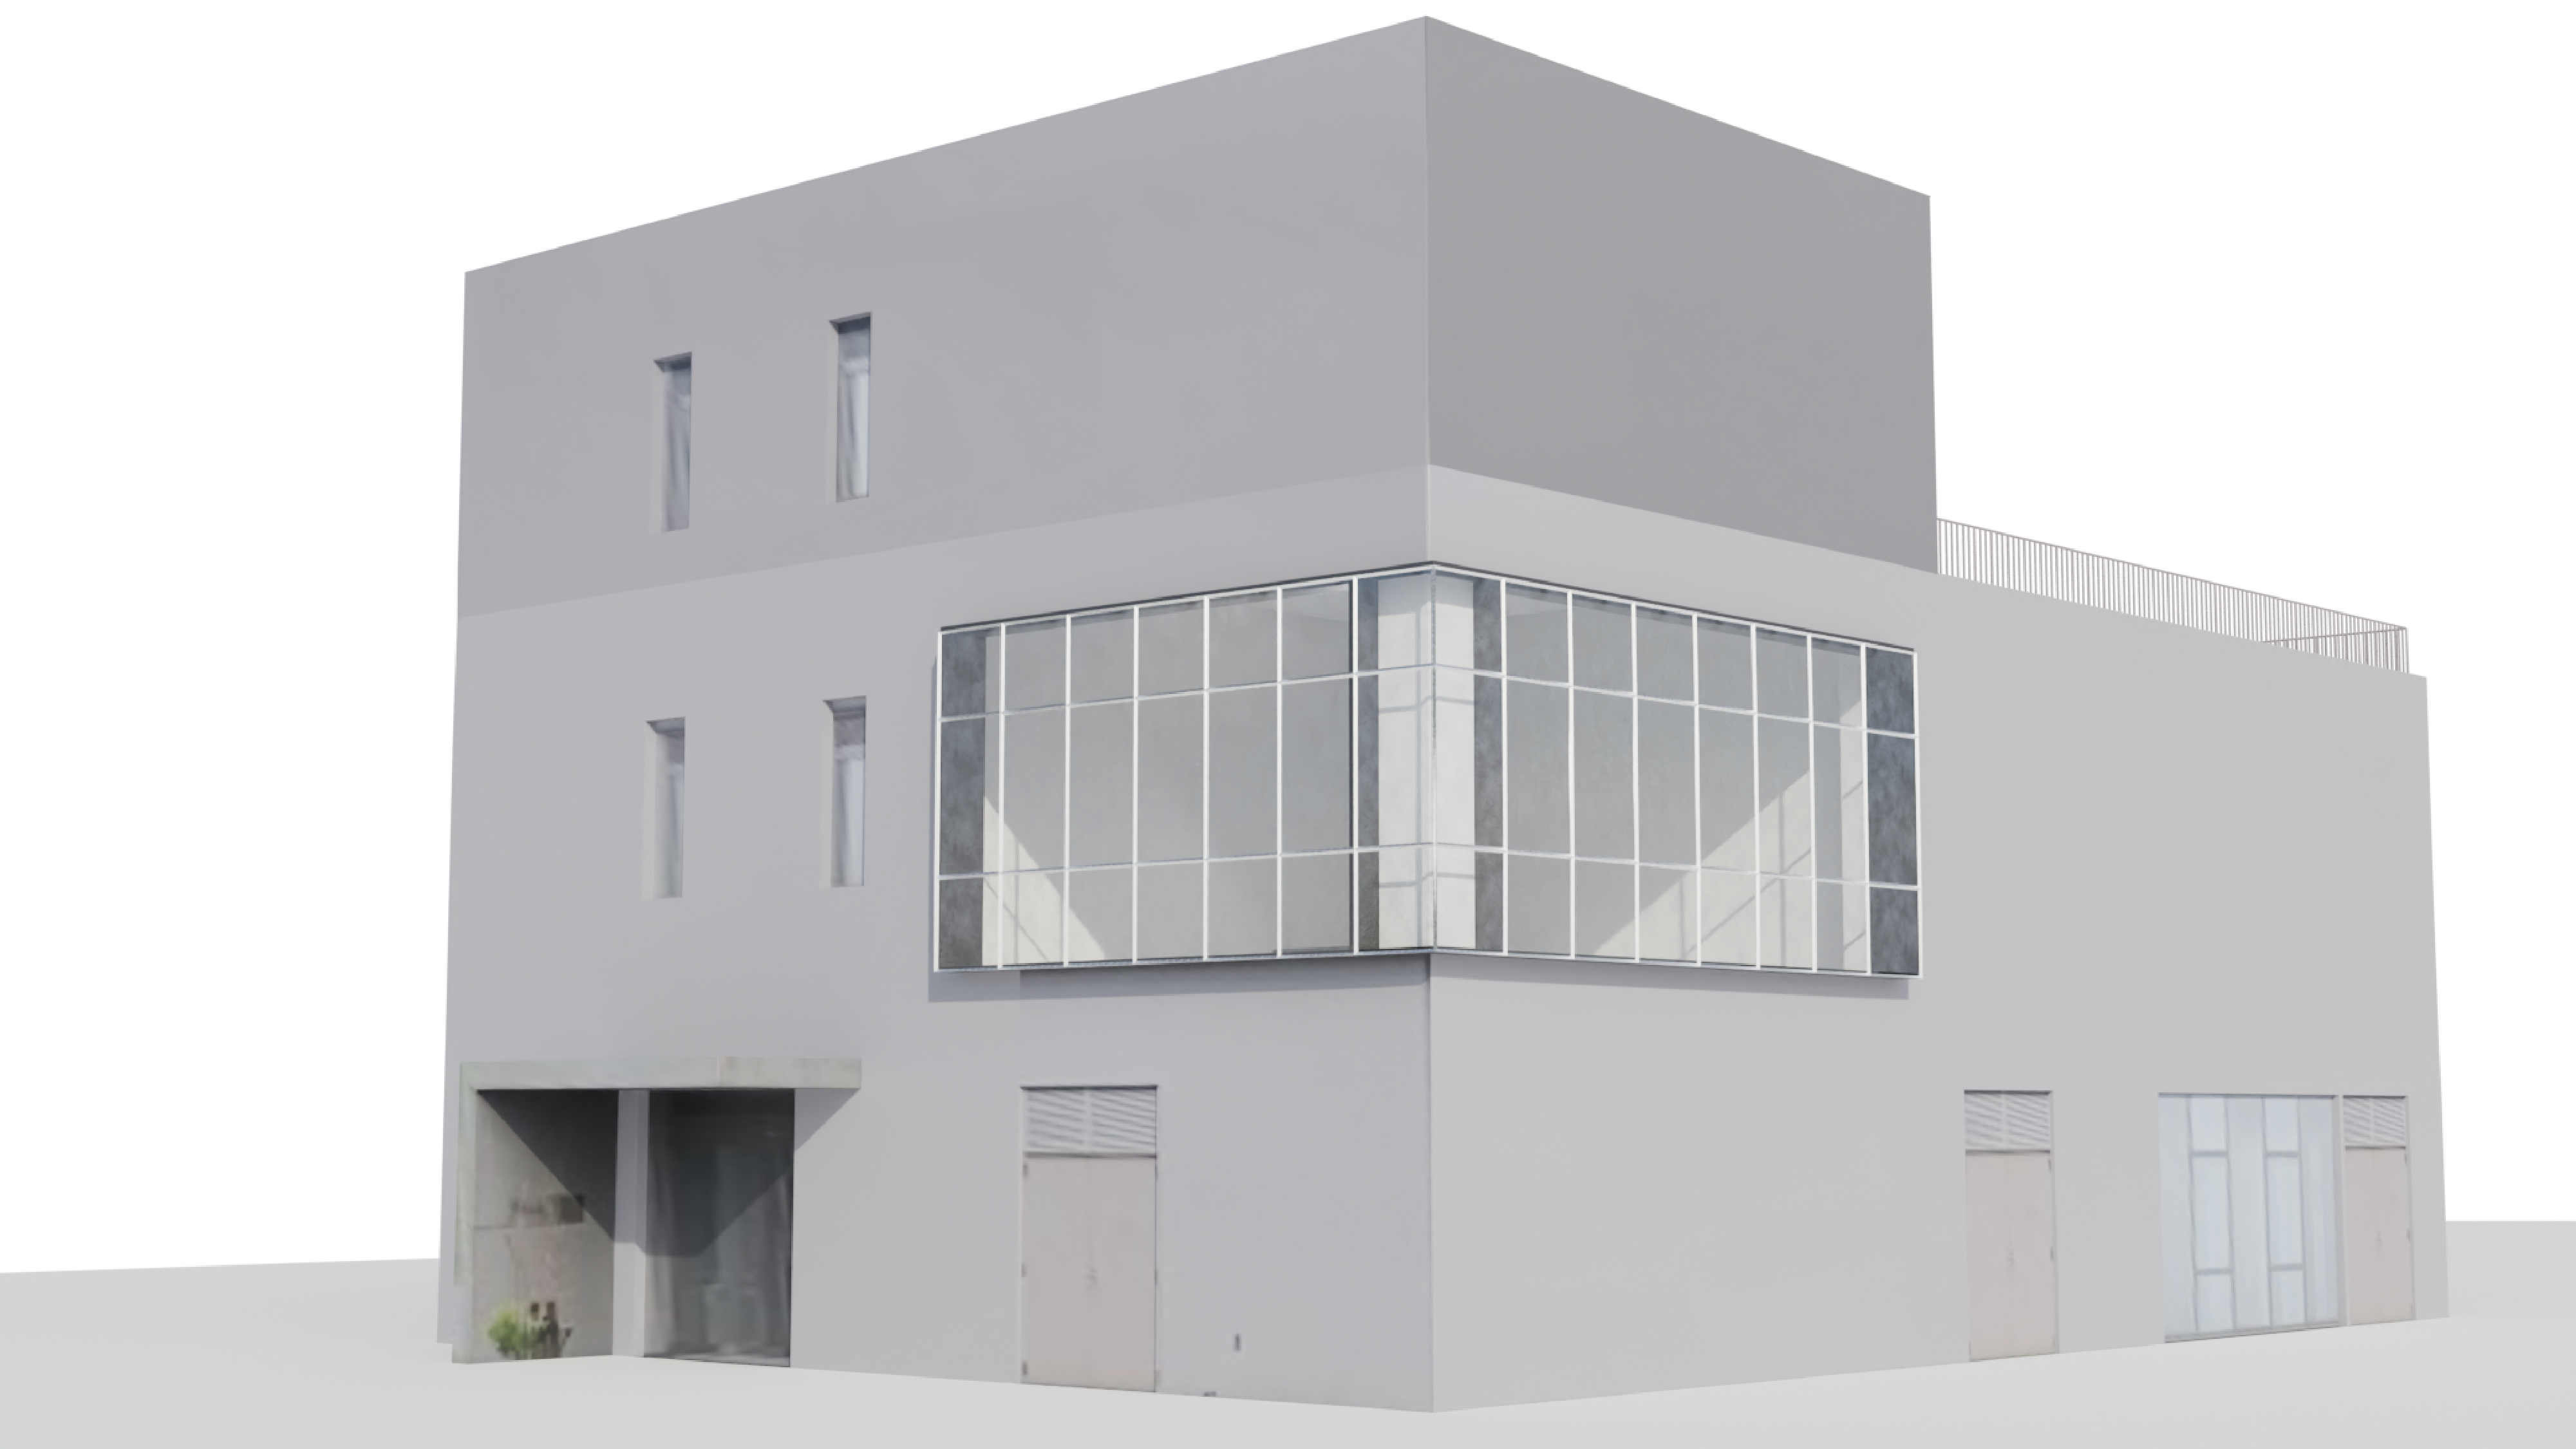
\includegraphics[width=1\linewidth]{Images/Base Module/Building}} &
              {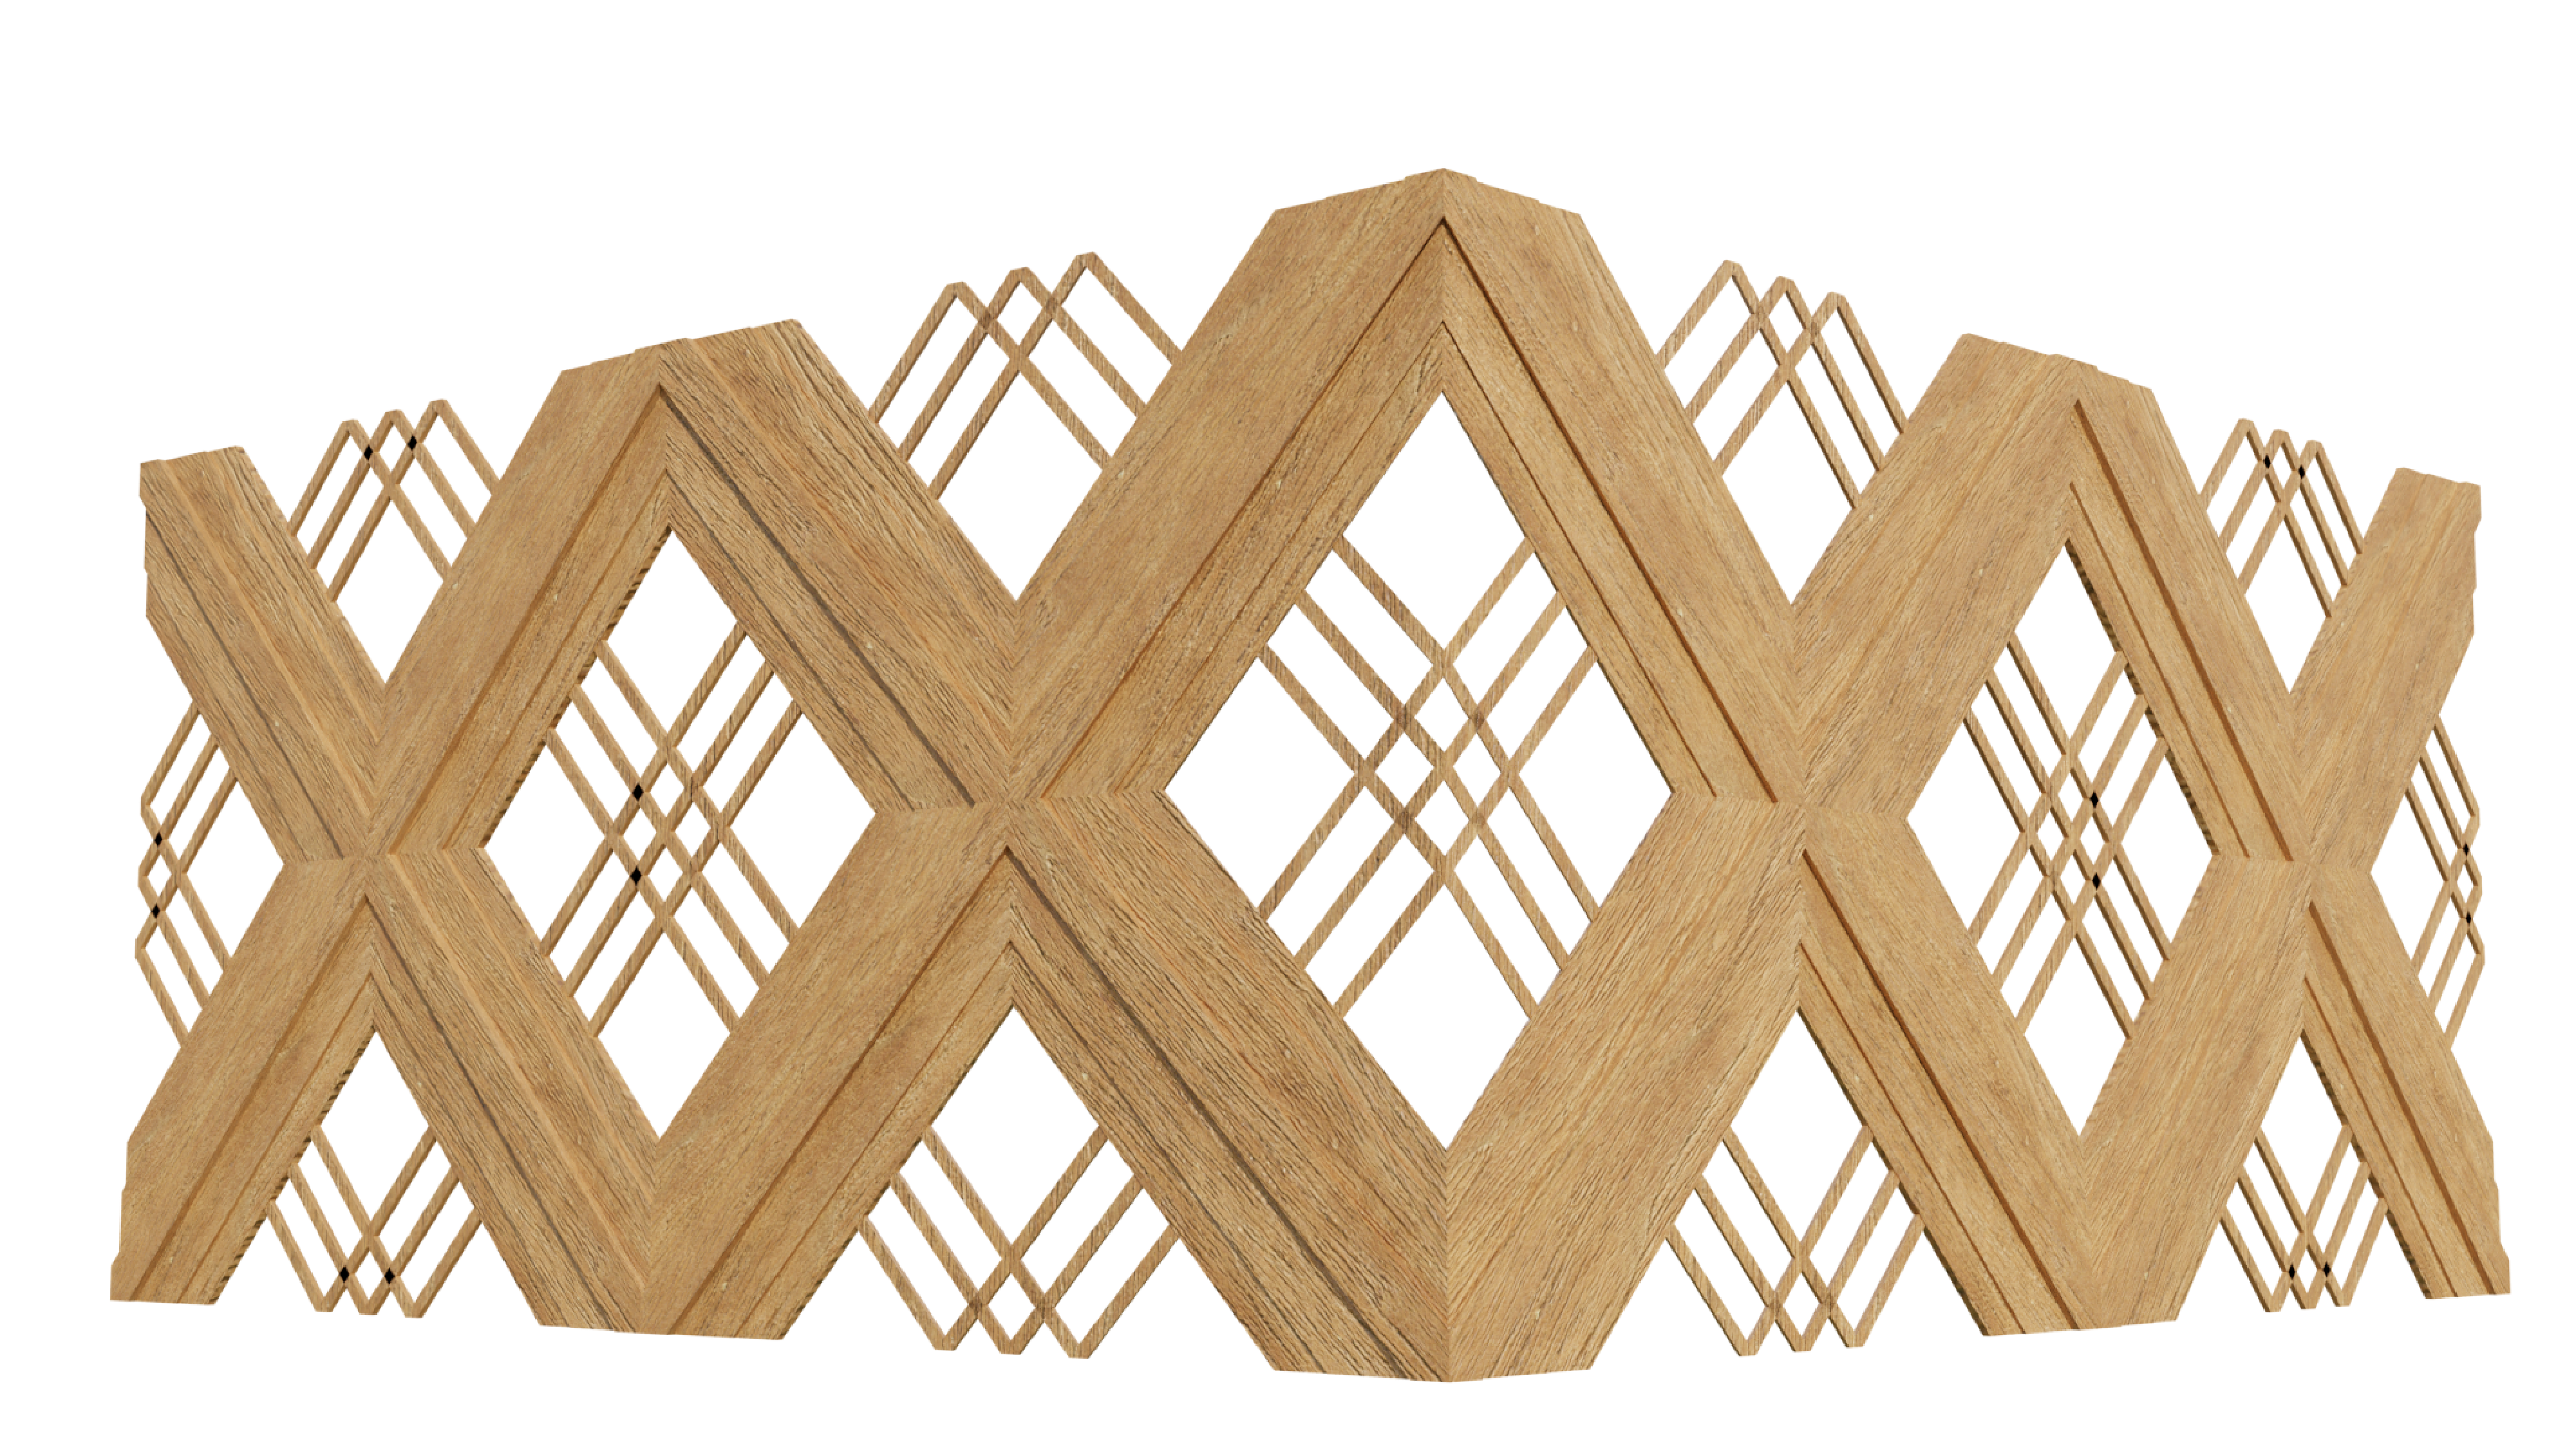
\includegraphics[width=1\linewidth]{Images/Base Module/Pattern1}} &
              {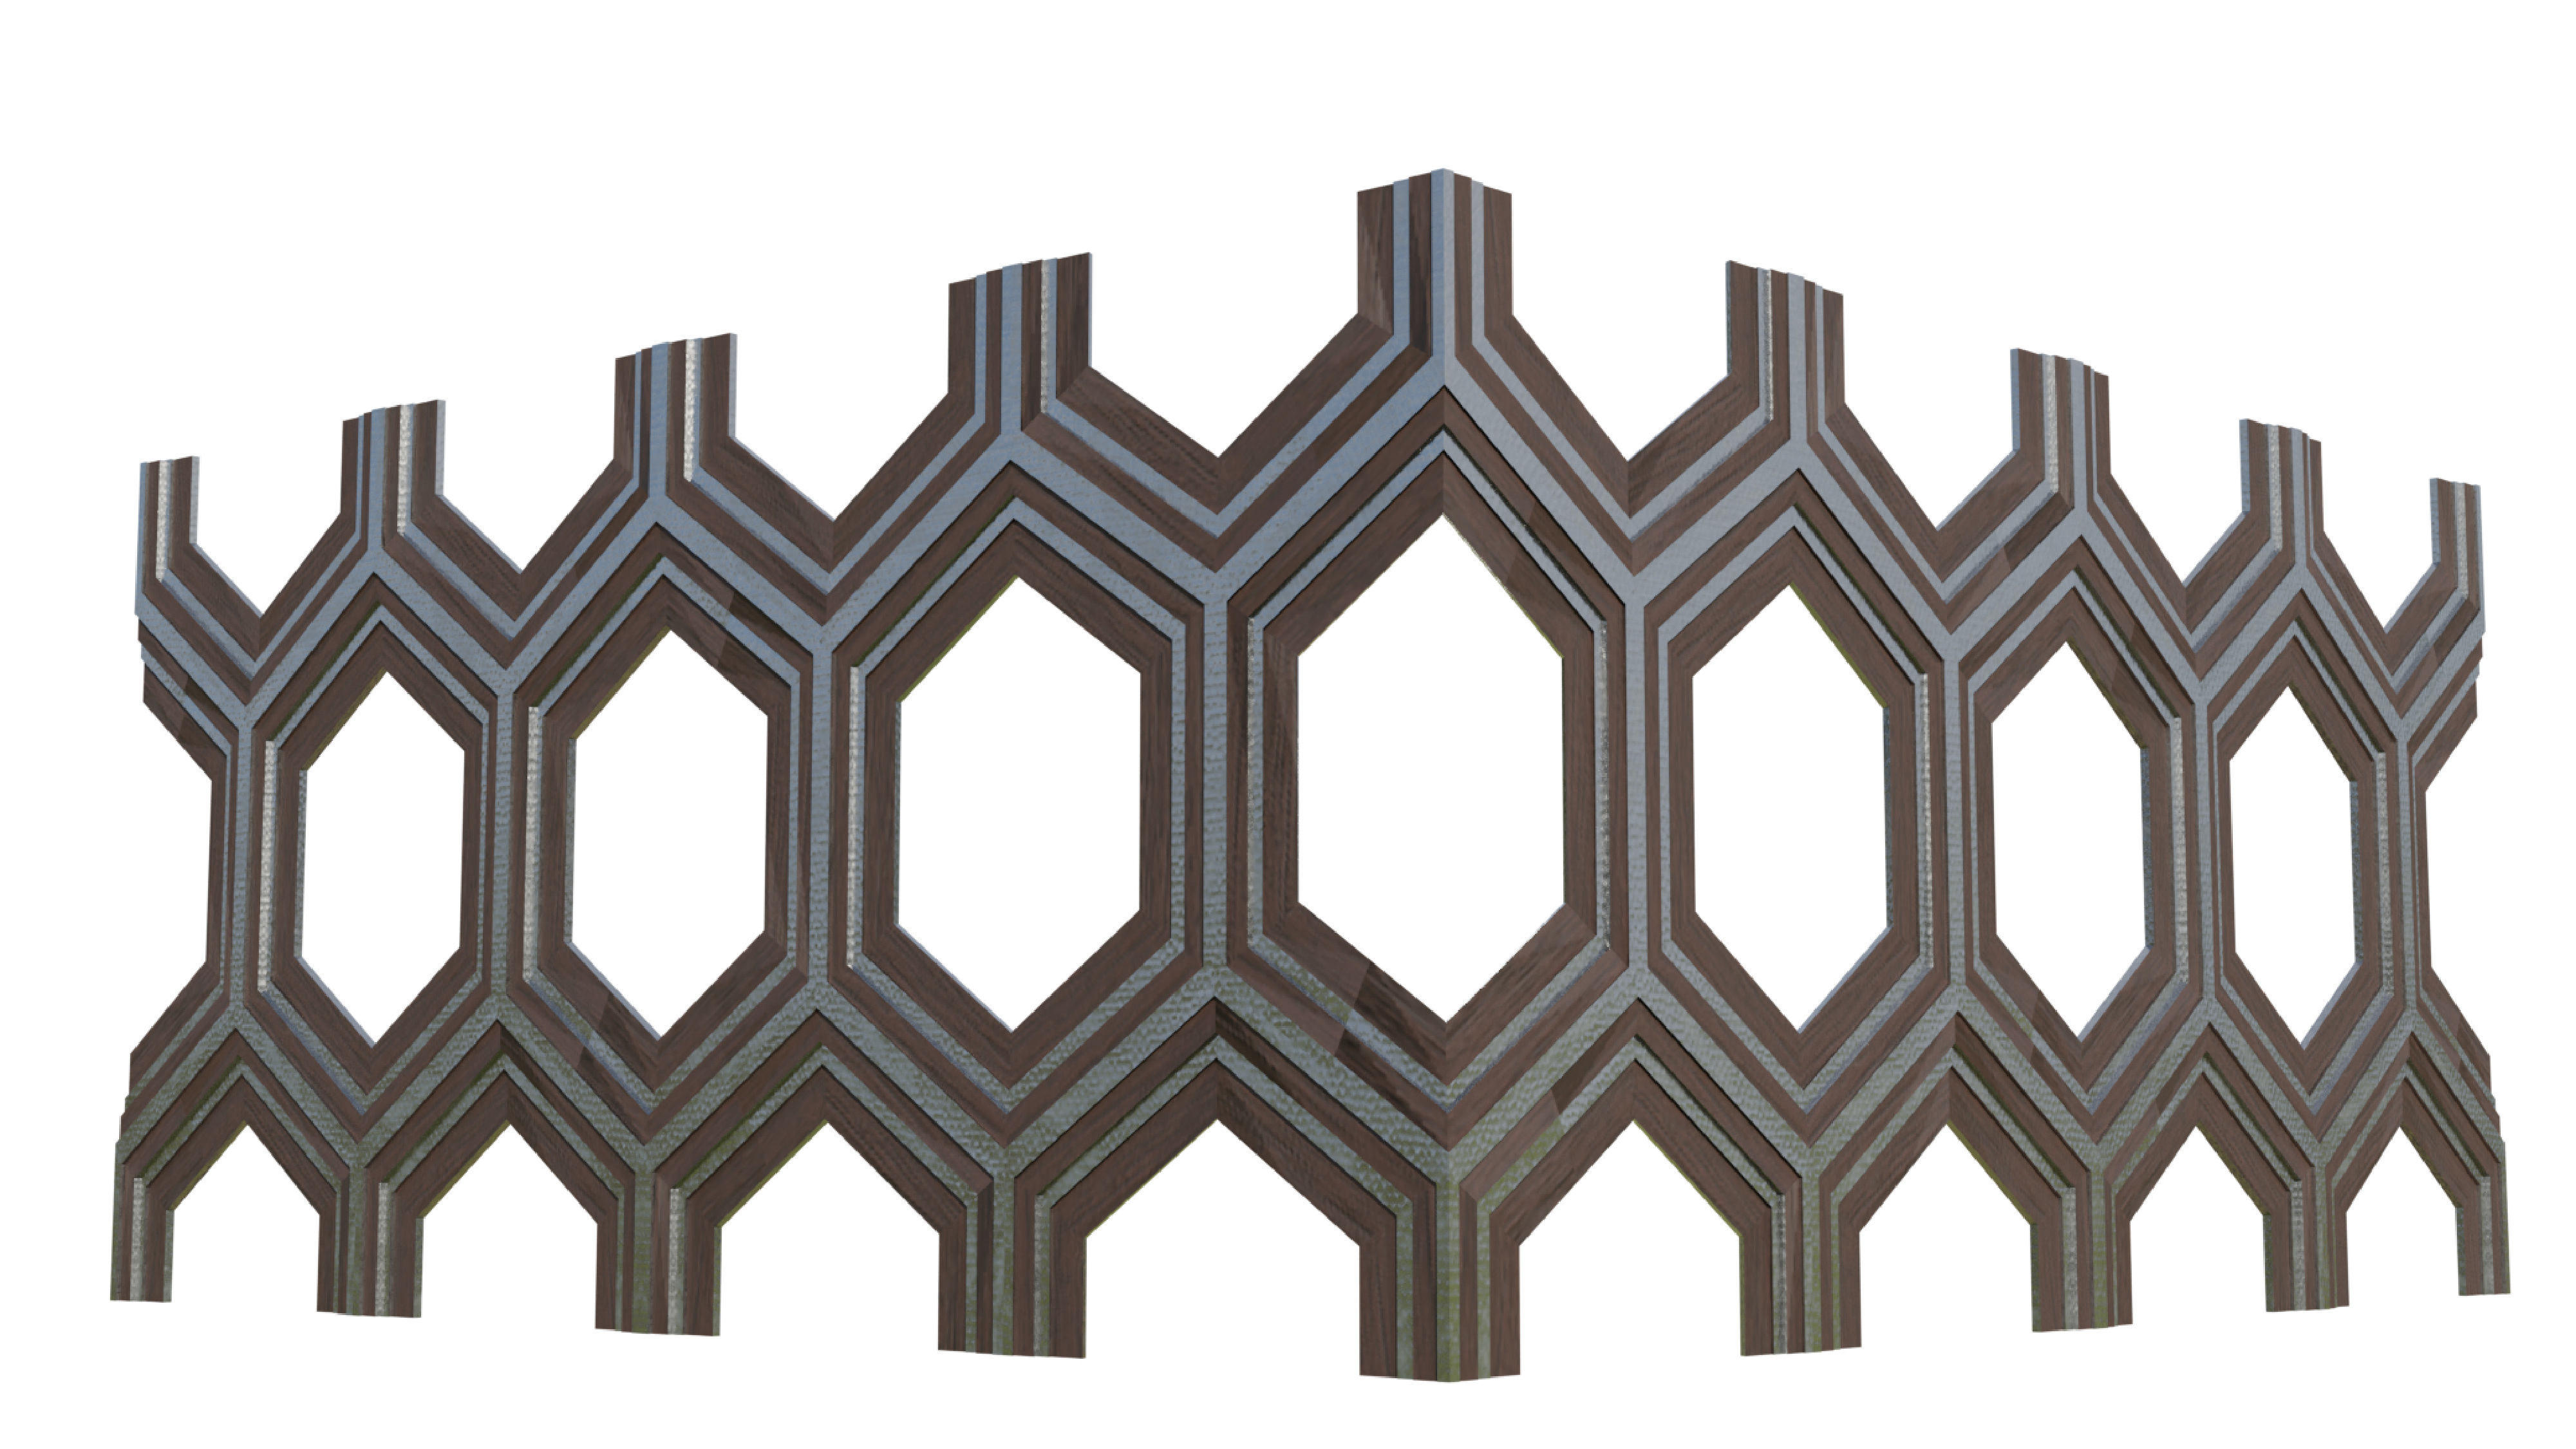
\includegraphics[width=1\linewidth]{Images/Base Module/Pattern2}} &
              {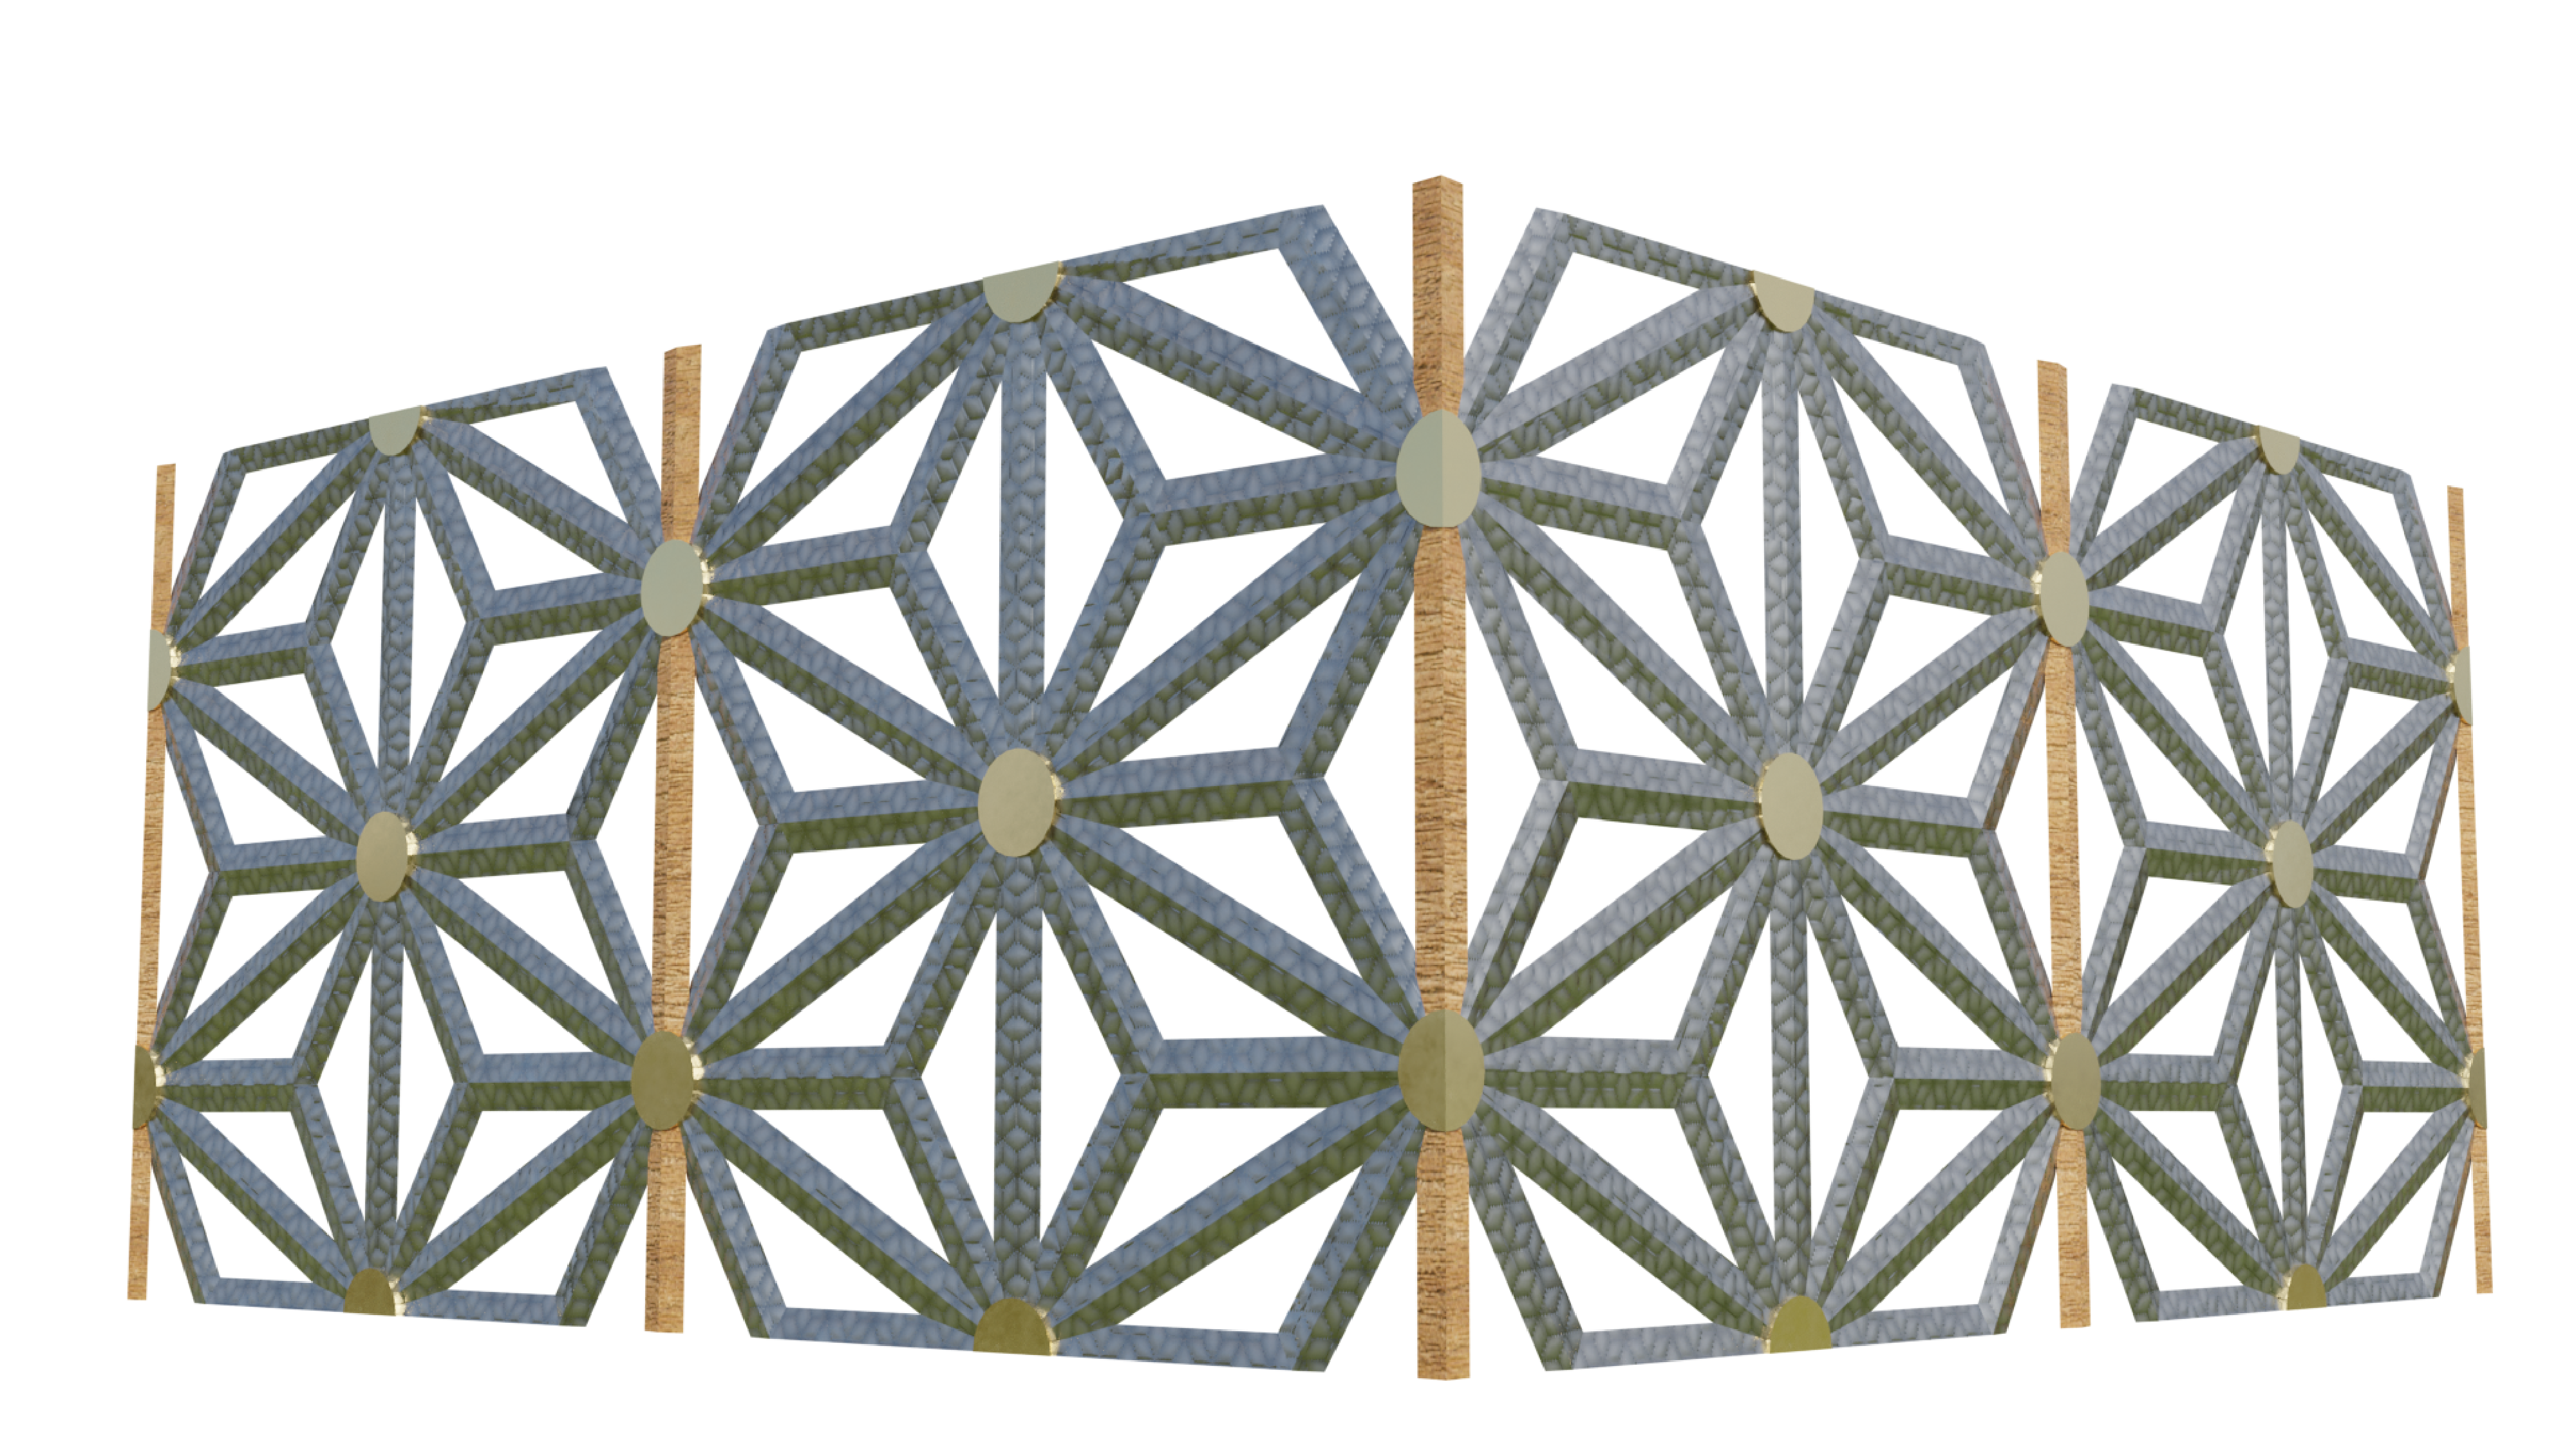
\includegraphics[width=1\linewidth]{Images/Base Module/Pattern3}} \\
            \midrule

            \textit{Mesh complexity Level} &
              \textit{Pattern 1} &
              \textit{Pattern 2} &
              \textit{Pattern 3}\\

            \midrule
            \textit{Level 1} &  &  &
            \\
            {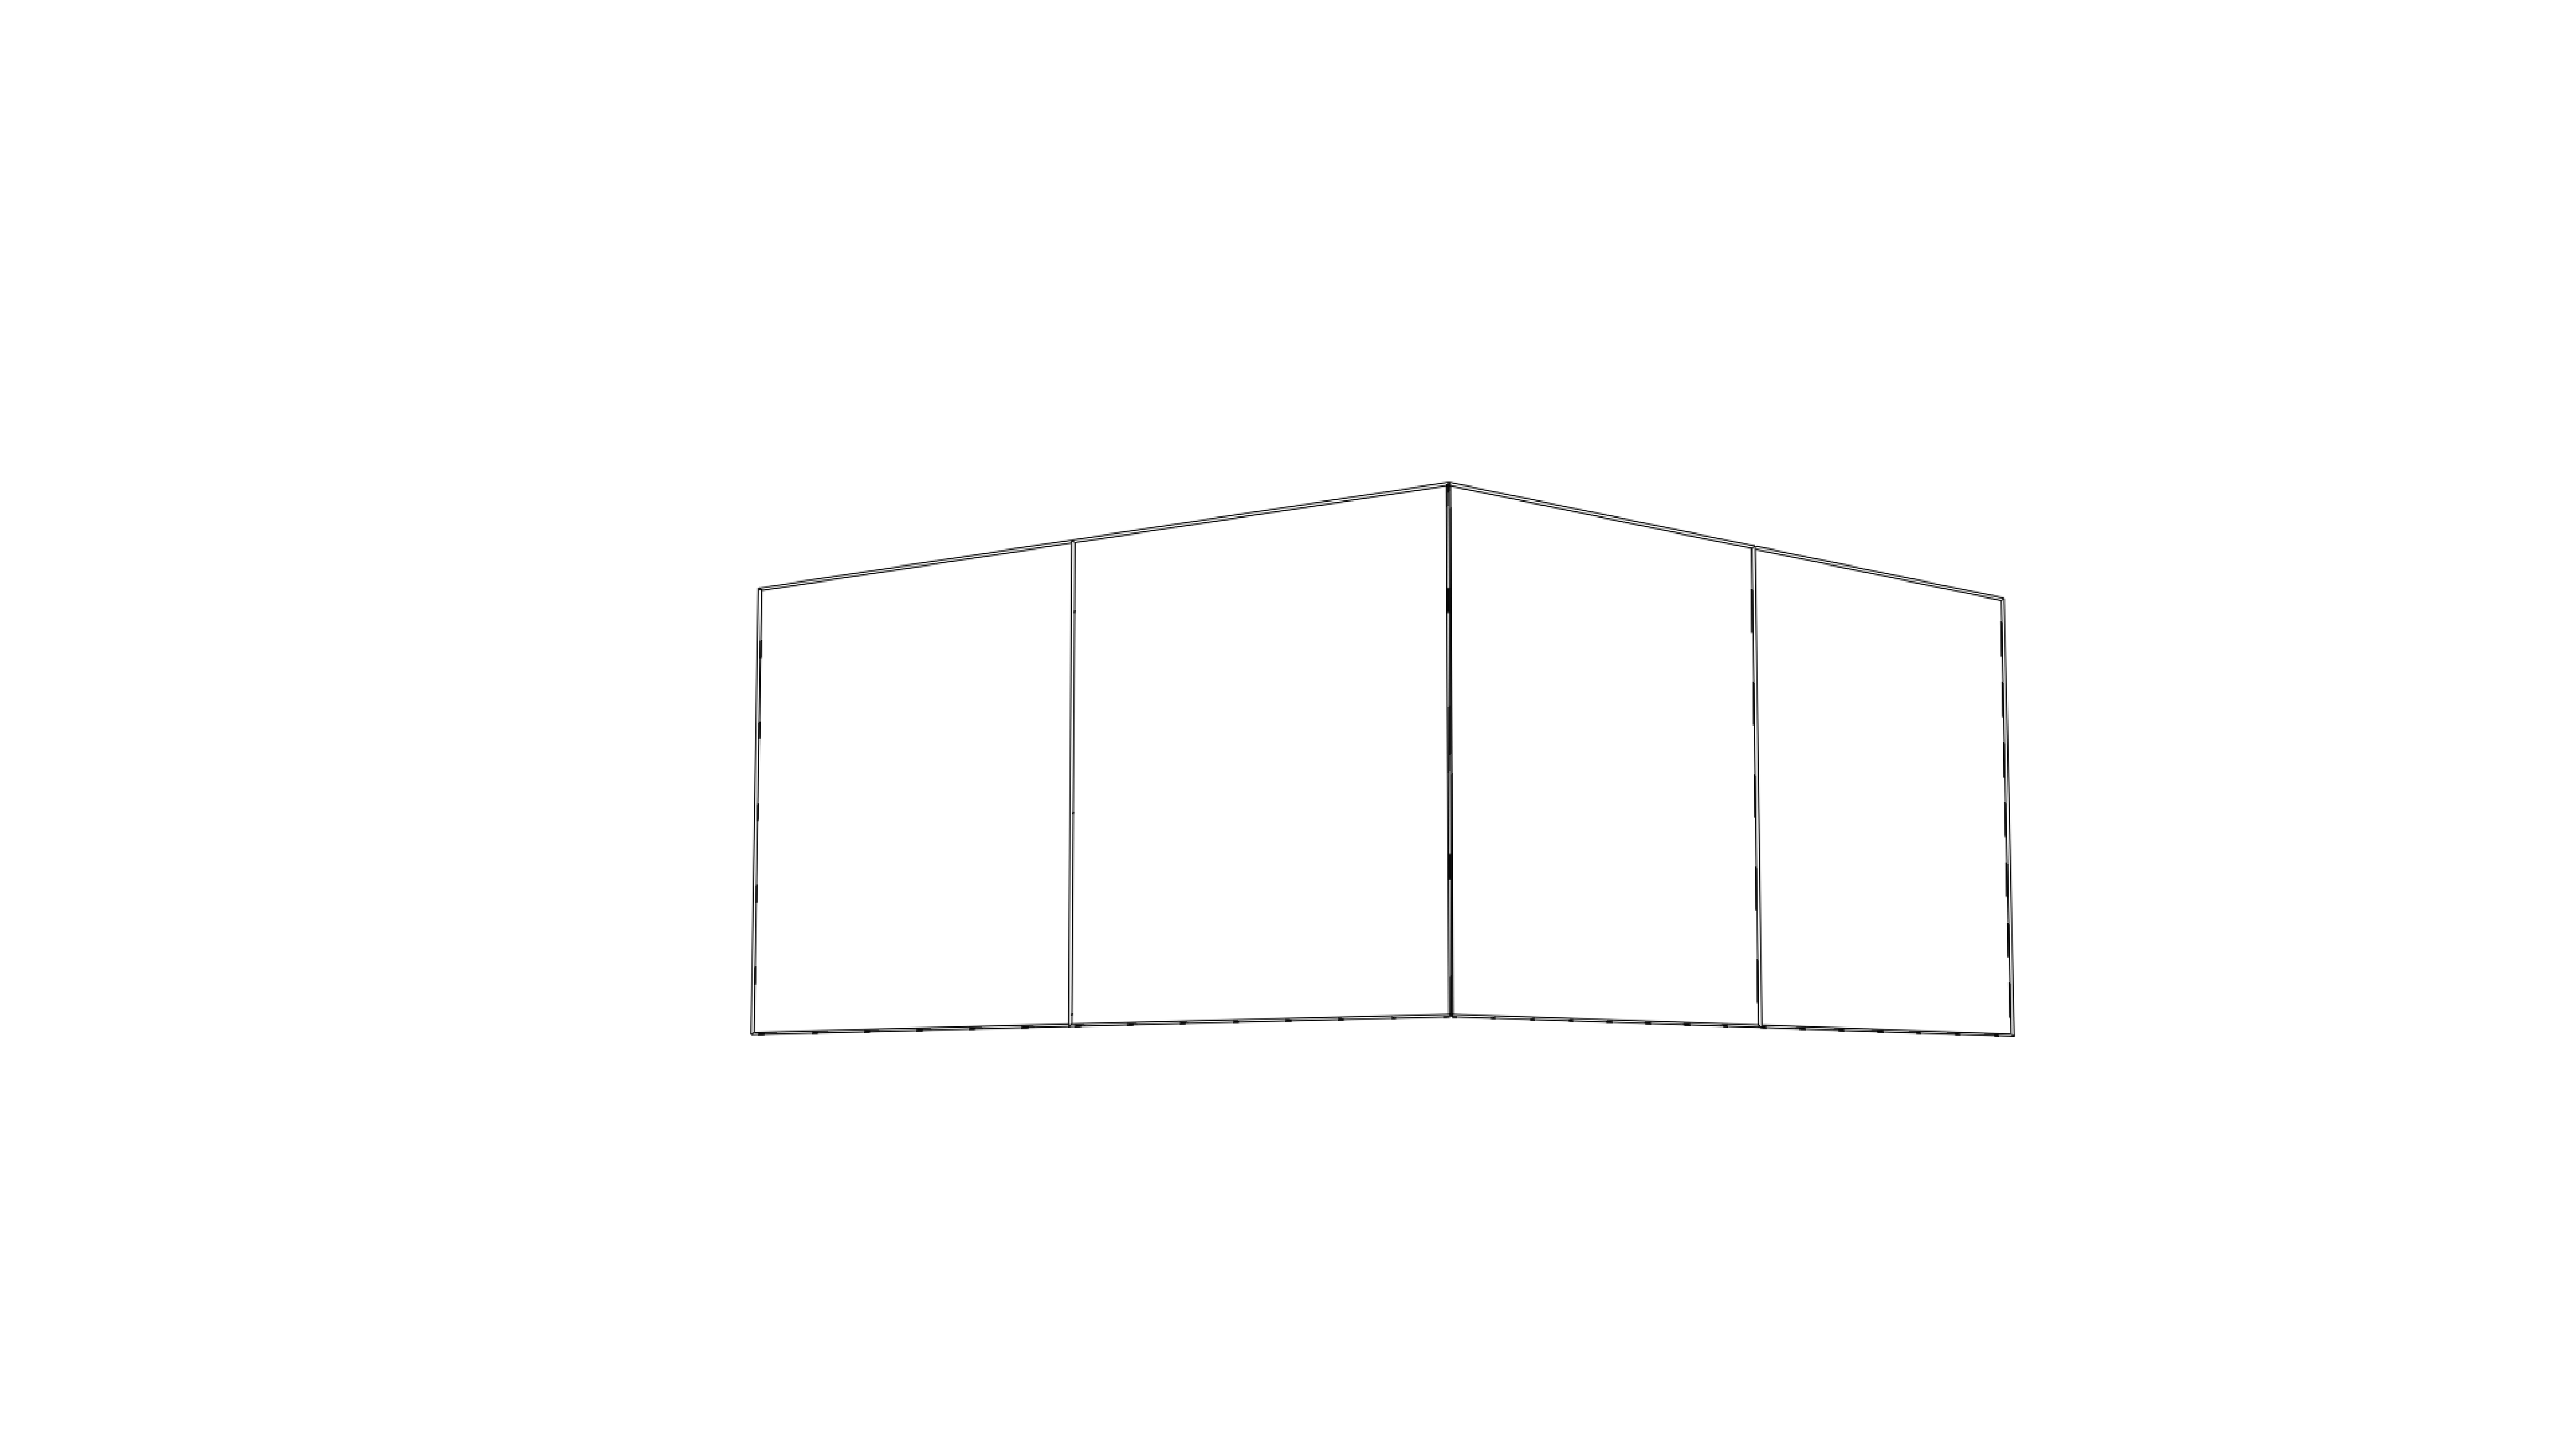
\includegraphics[width=1\linewidth]{Images/Wall 0/0001}} &
                {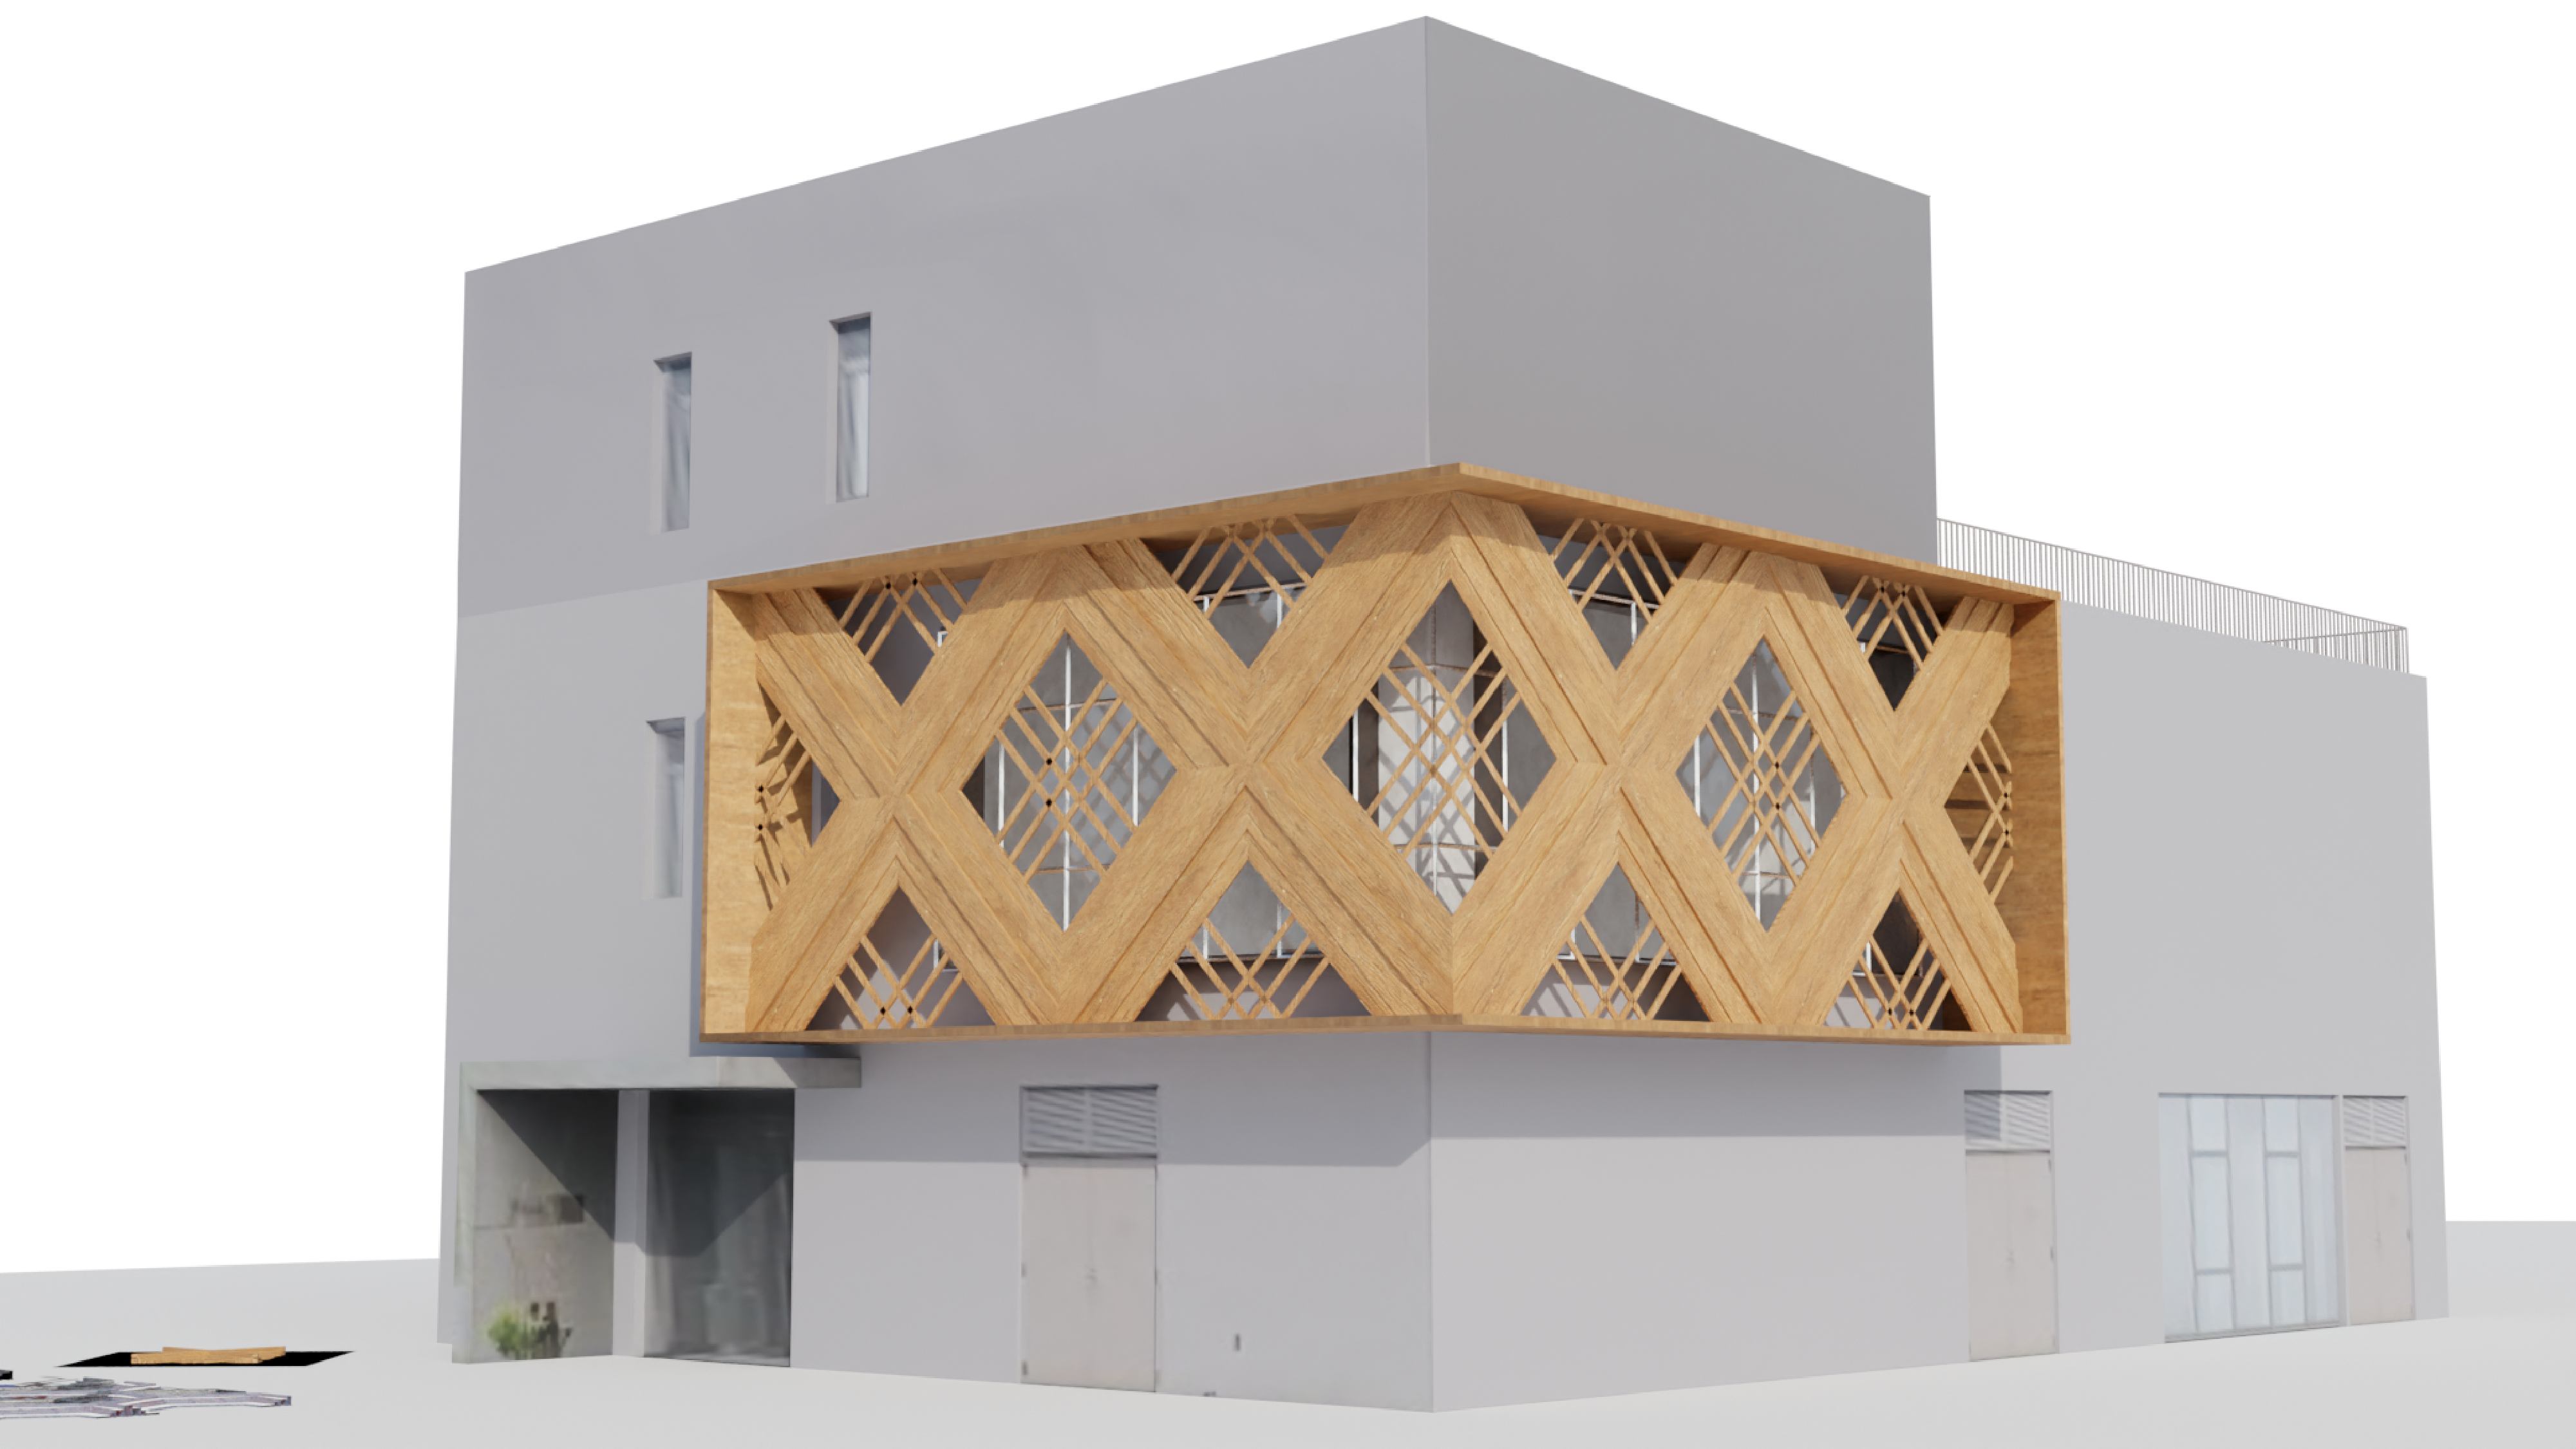
\includegraphics[width=1\linewidth]{Images/Pattern 1/0001}} &
              {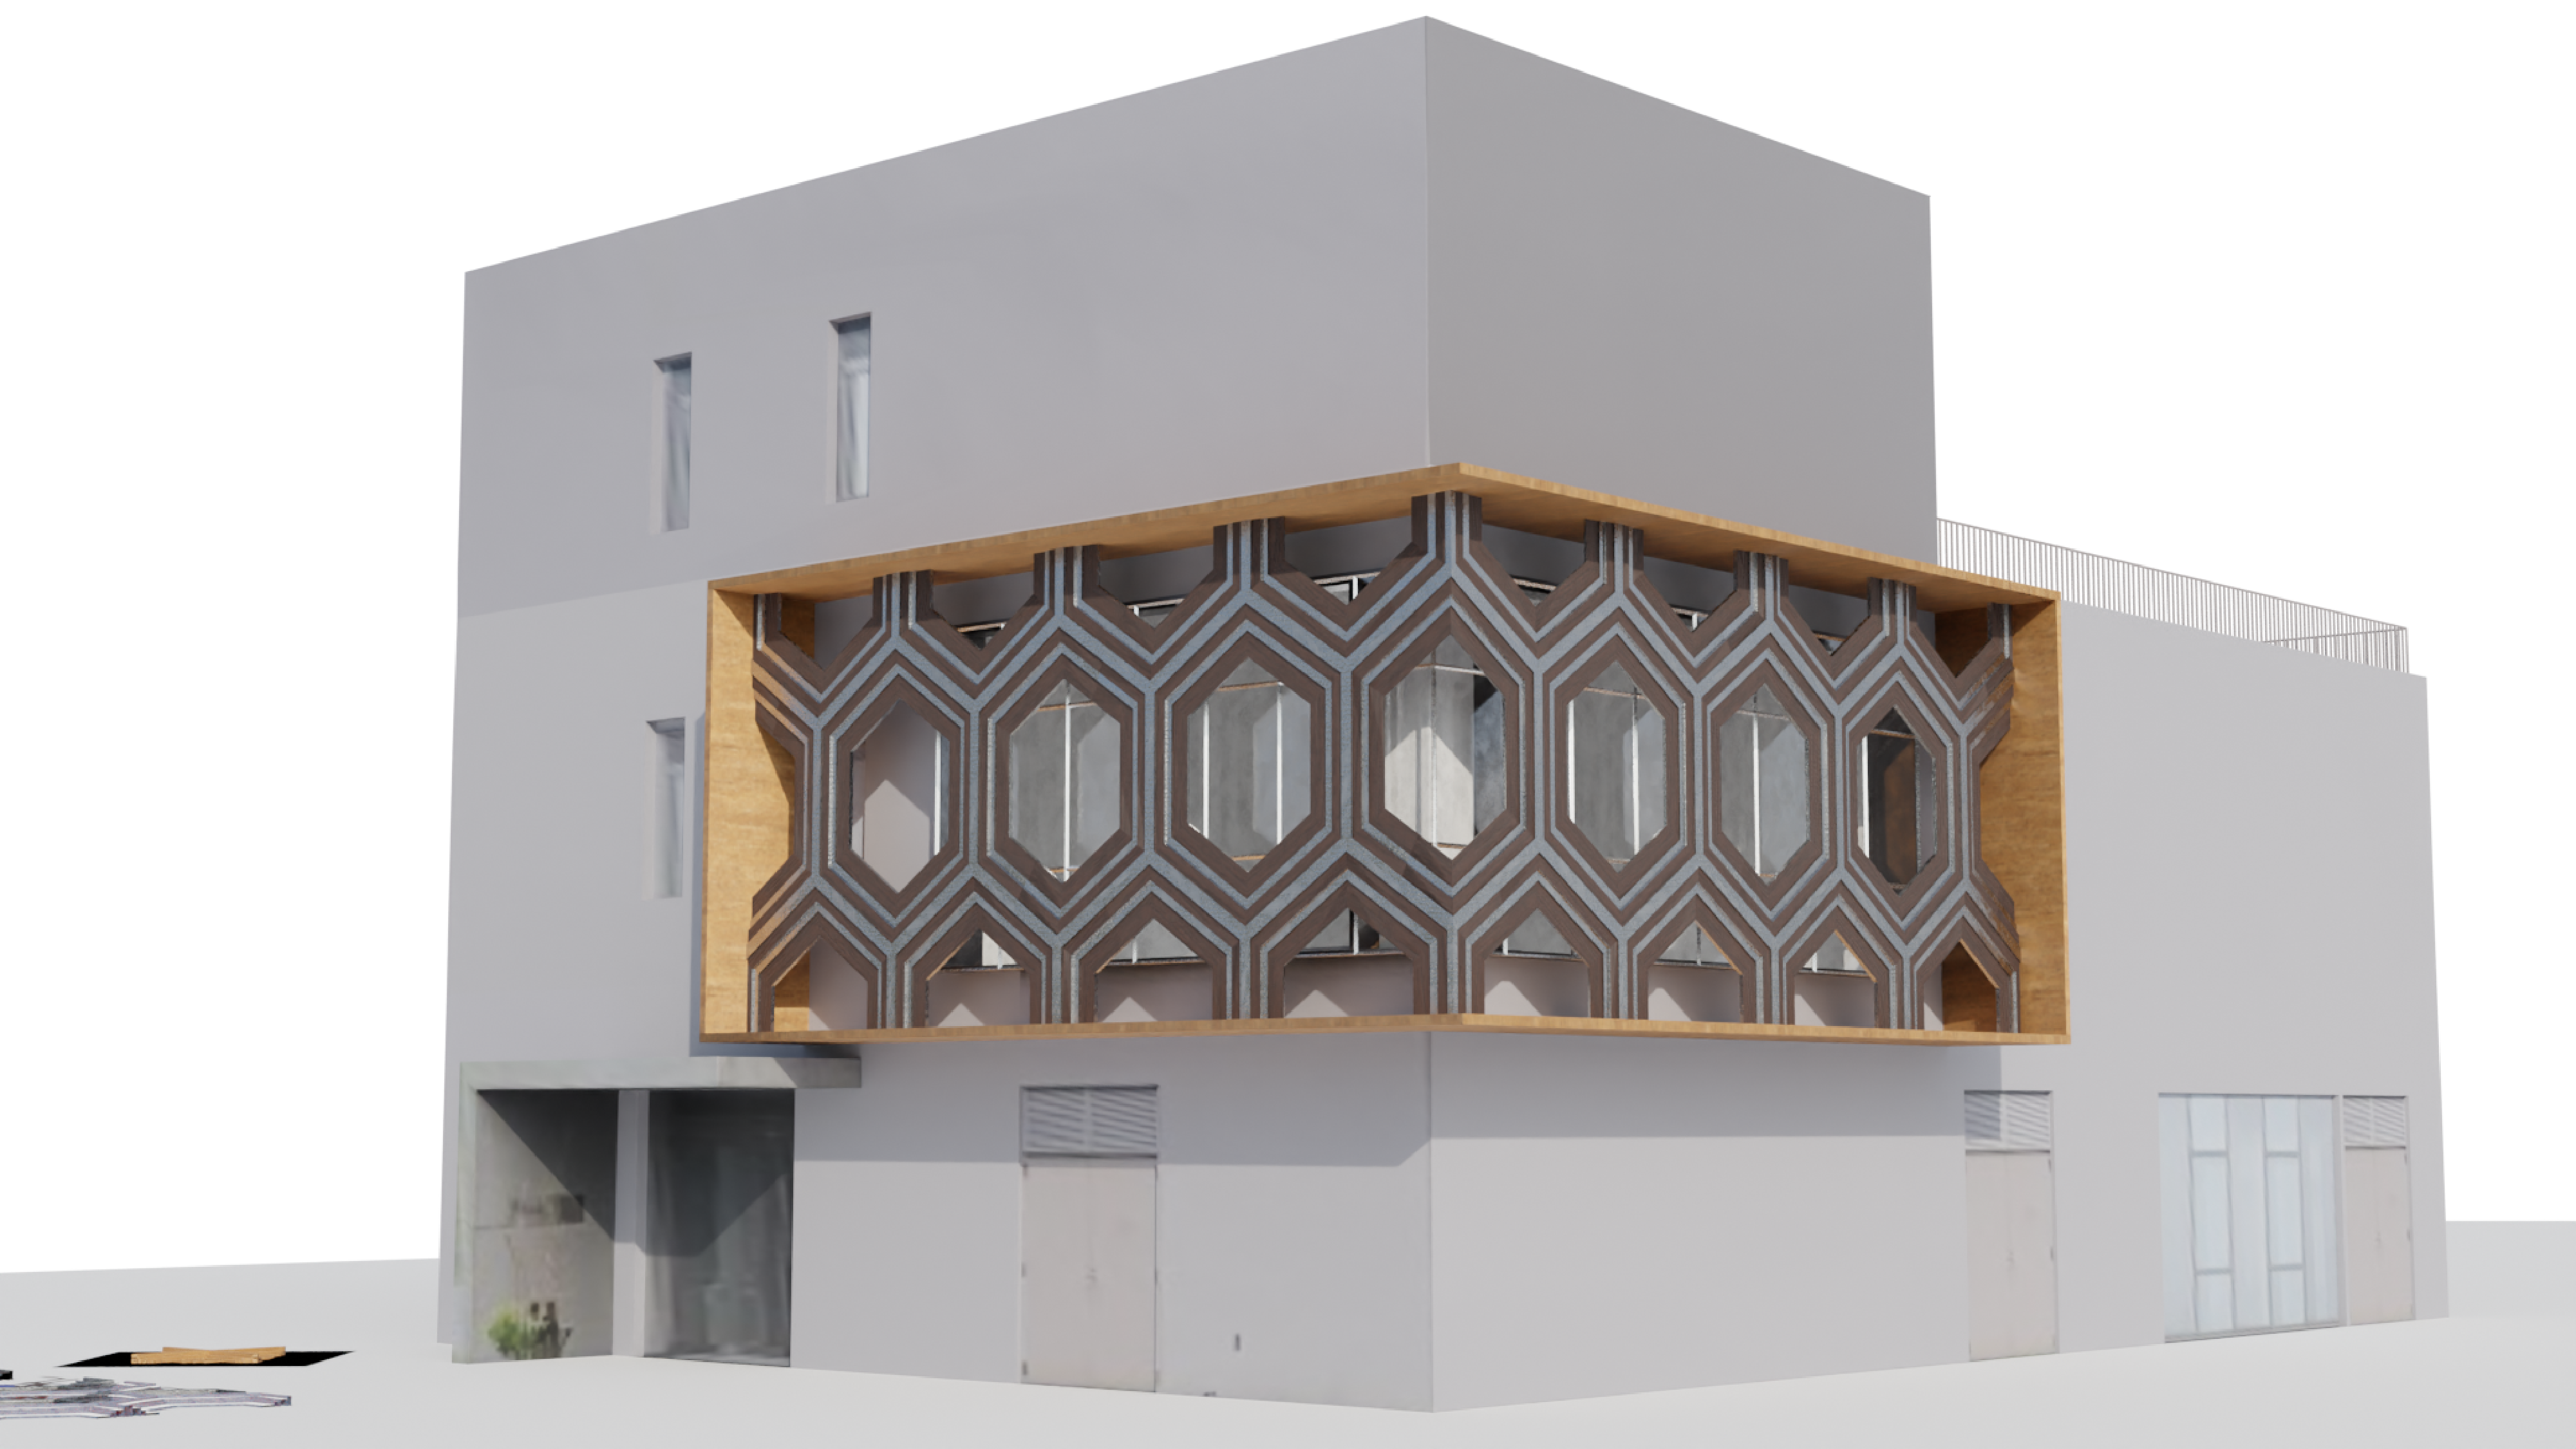
\includegraphics[width=1\linewidth]{Images/Pattern 2/0001}} &
              {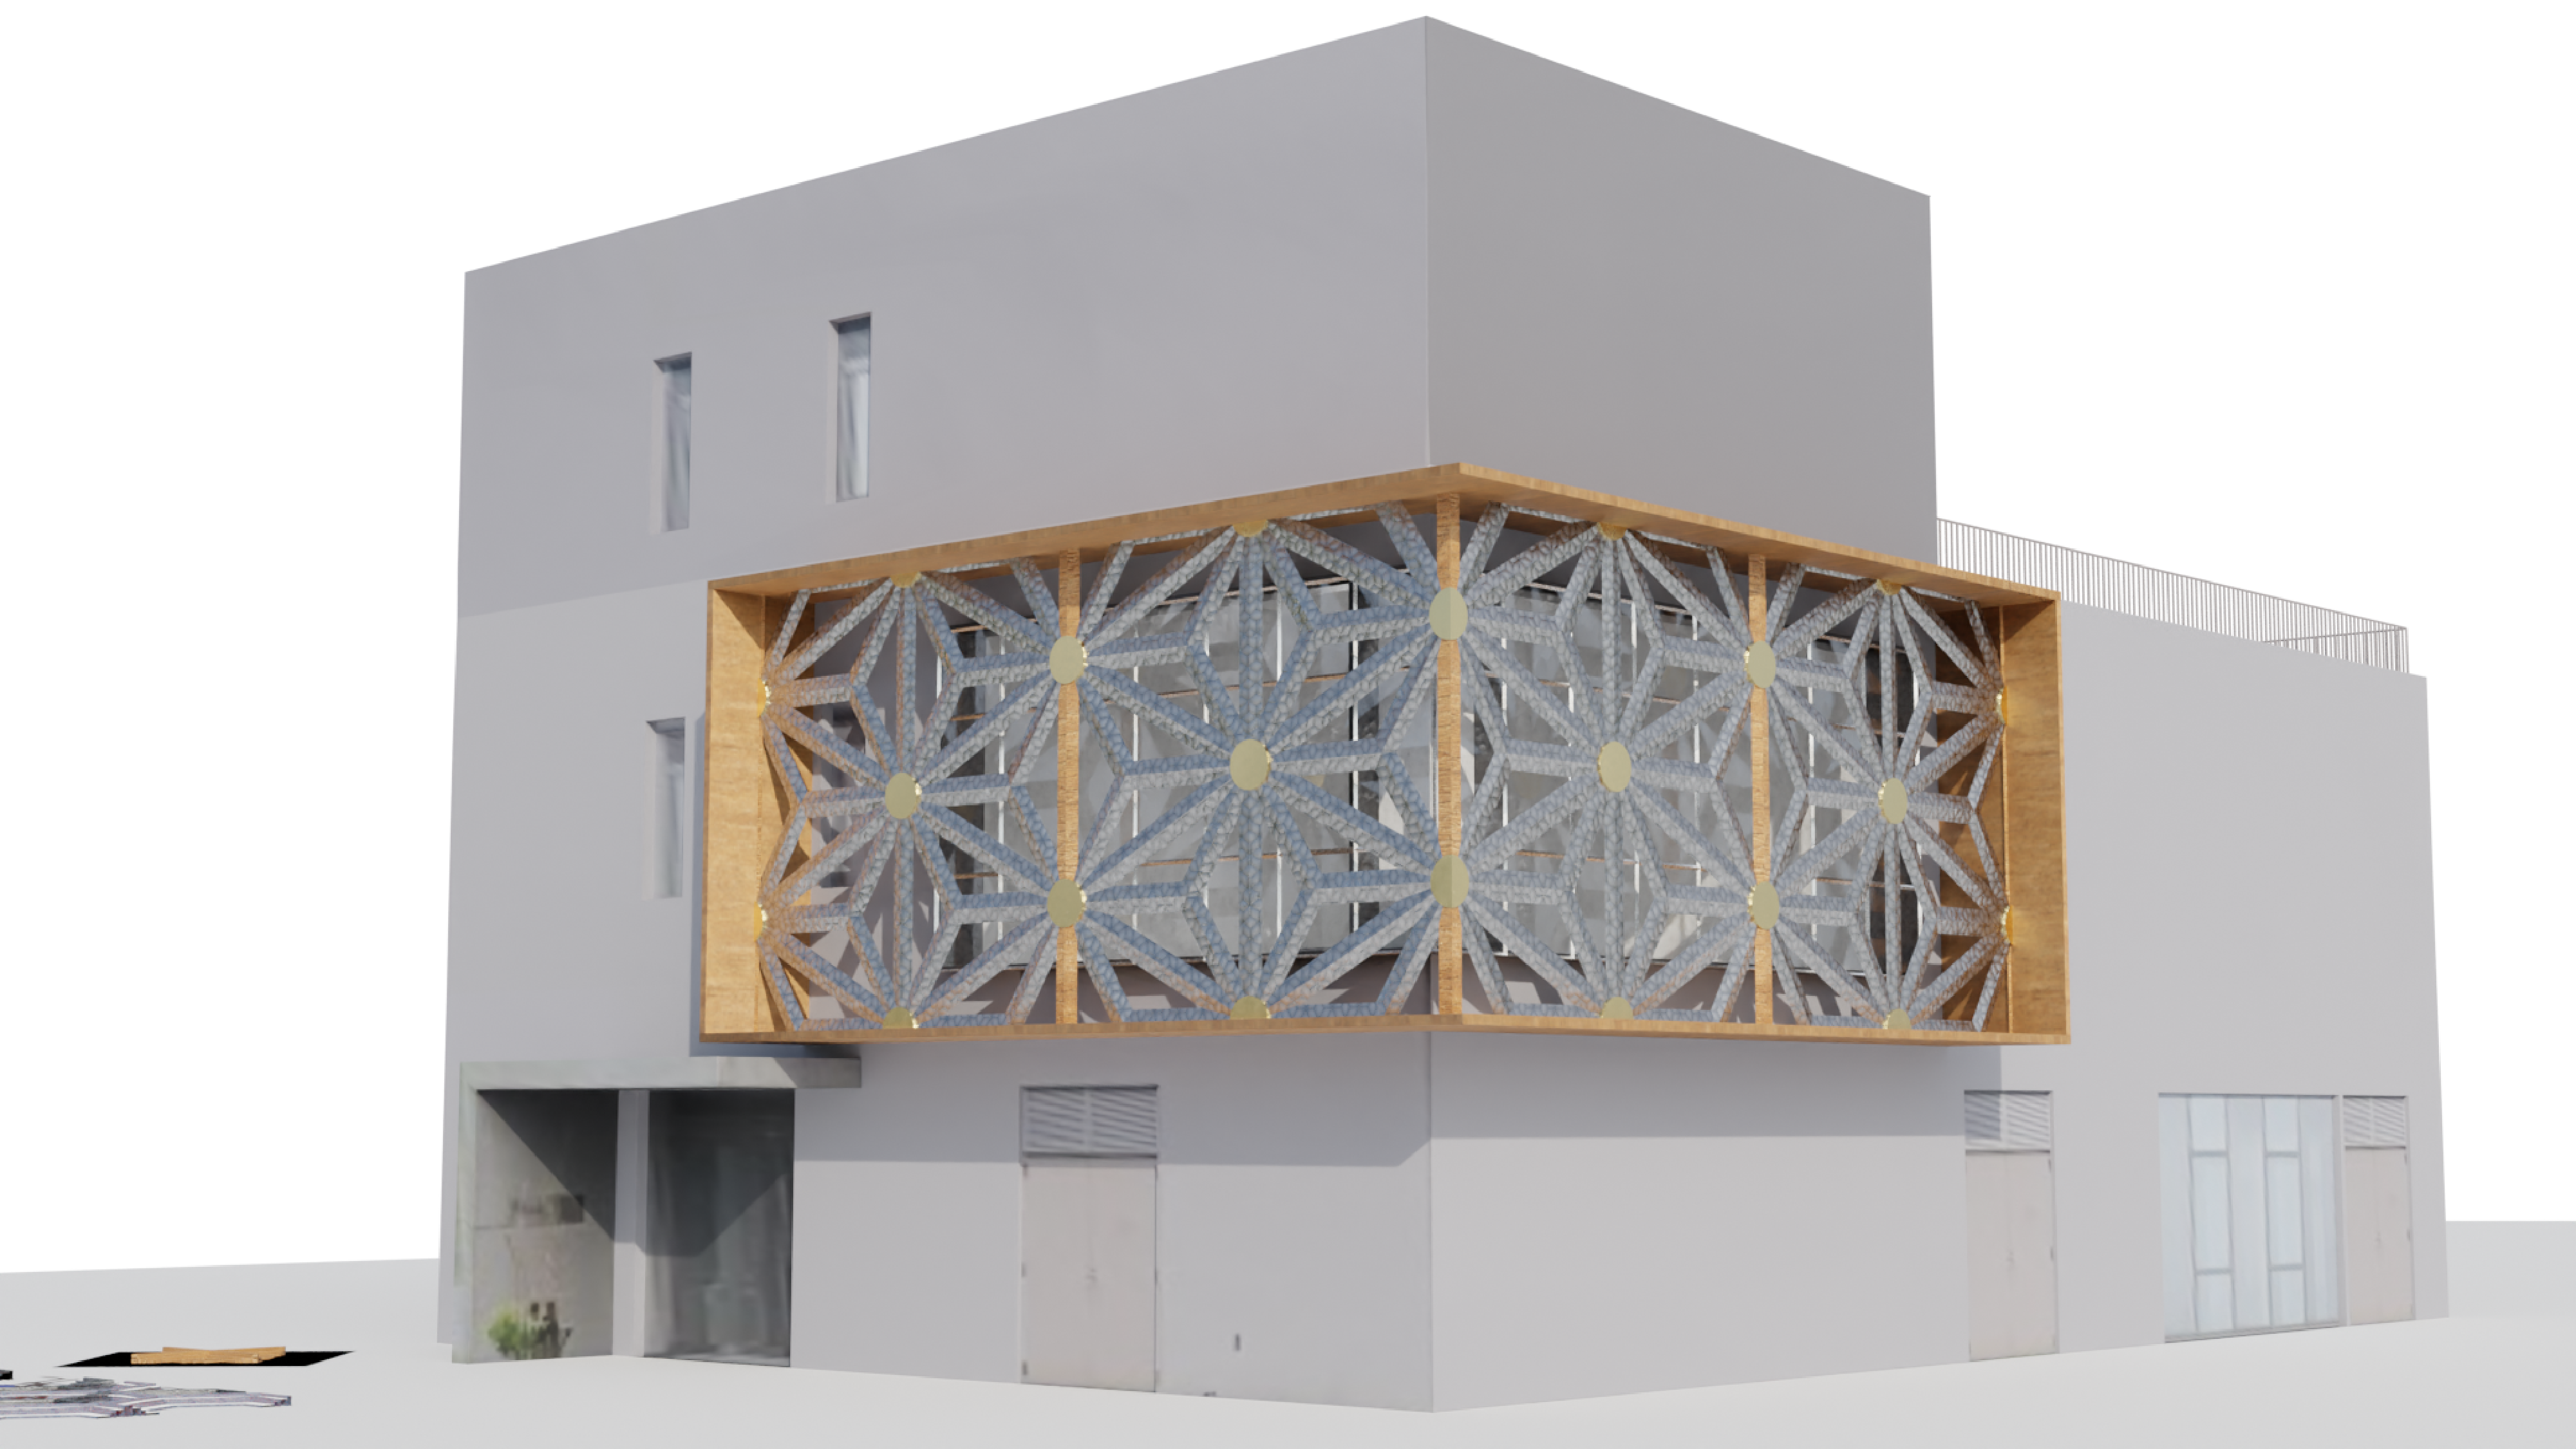
\includegraphics[width=1\linewidth]{Images/Pattern 3/0001}} \\
            \midrule
            \textit{Level 2} &  &  &
            \\
            {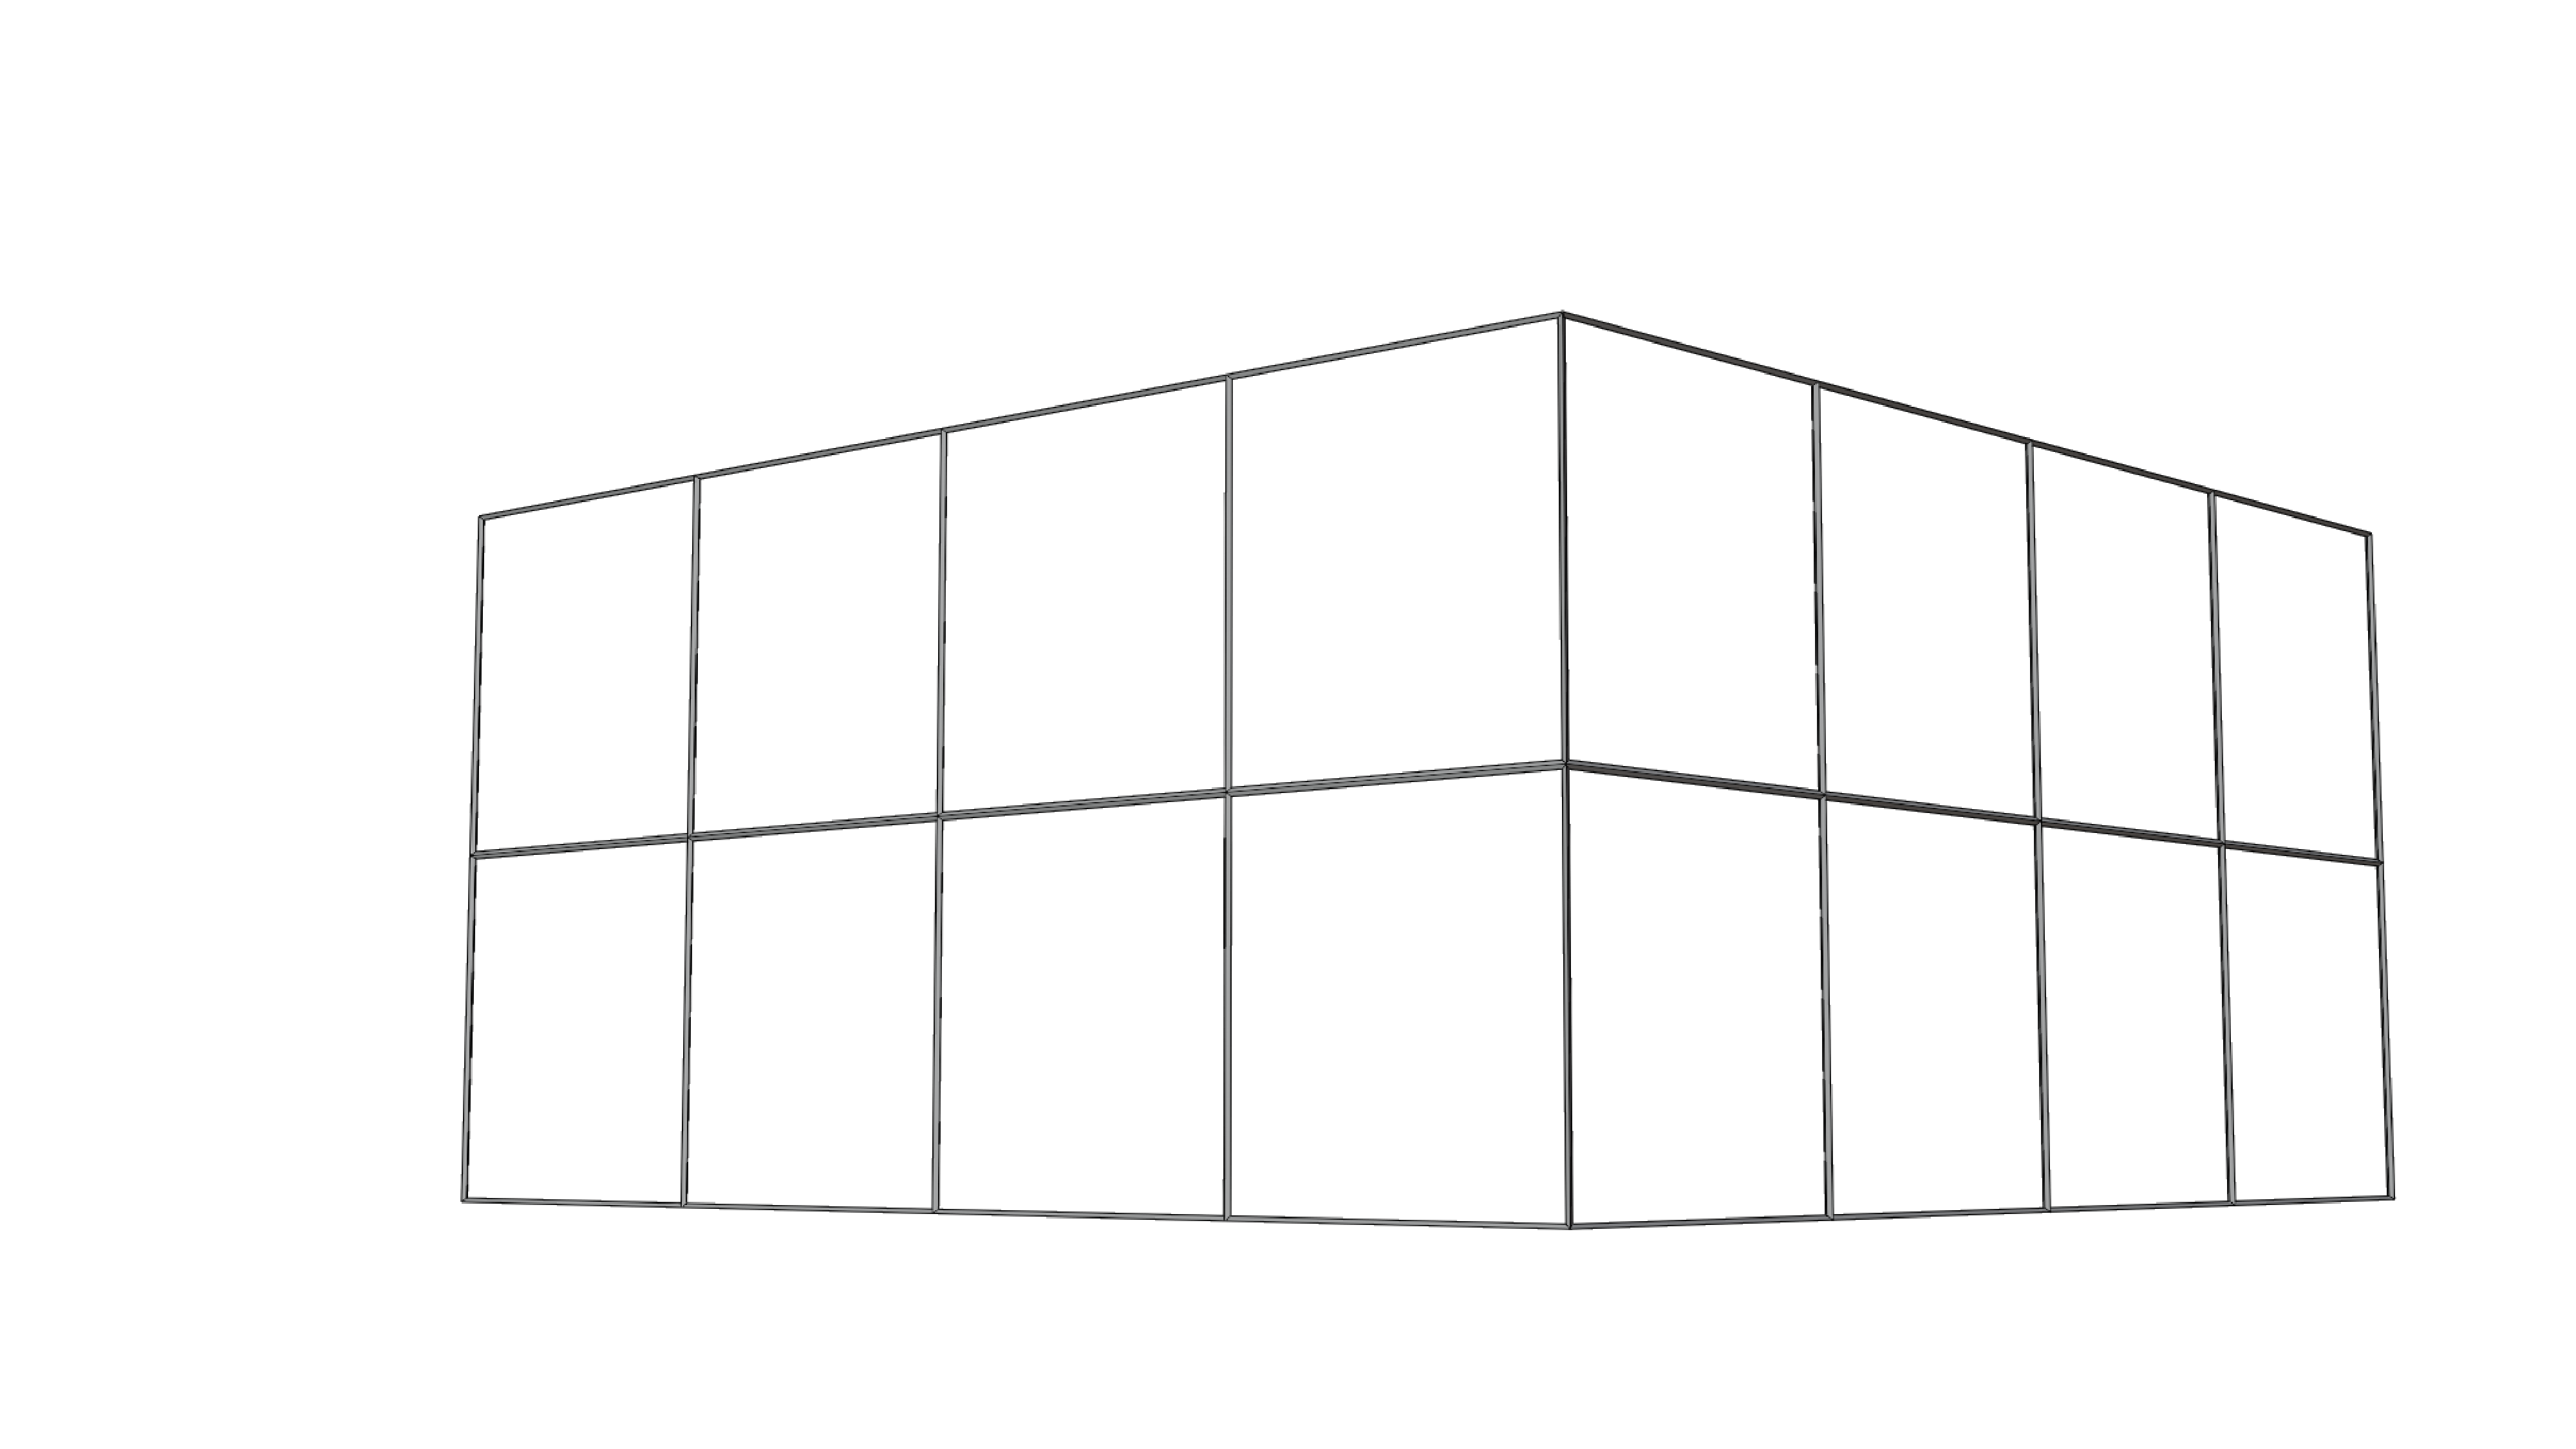
\includegraphics[width=1\linewidth]{Images/Wall 0/0002}} &
              {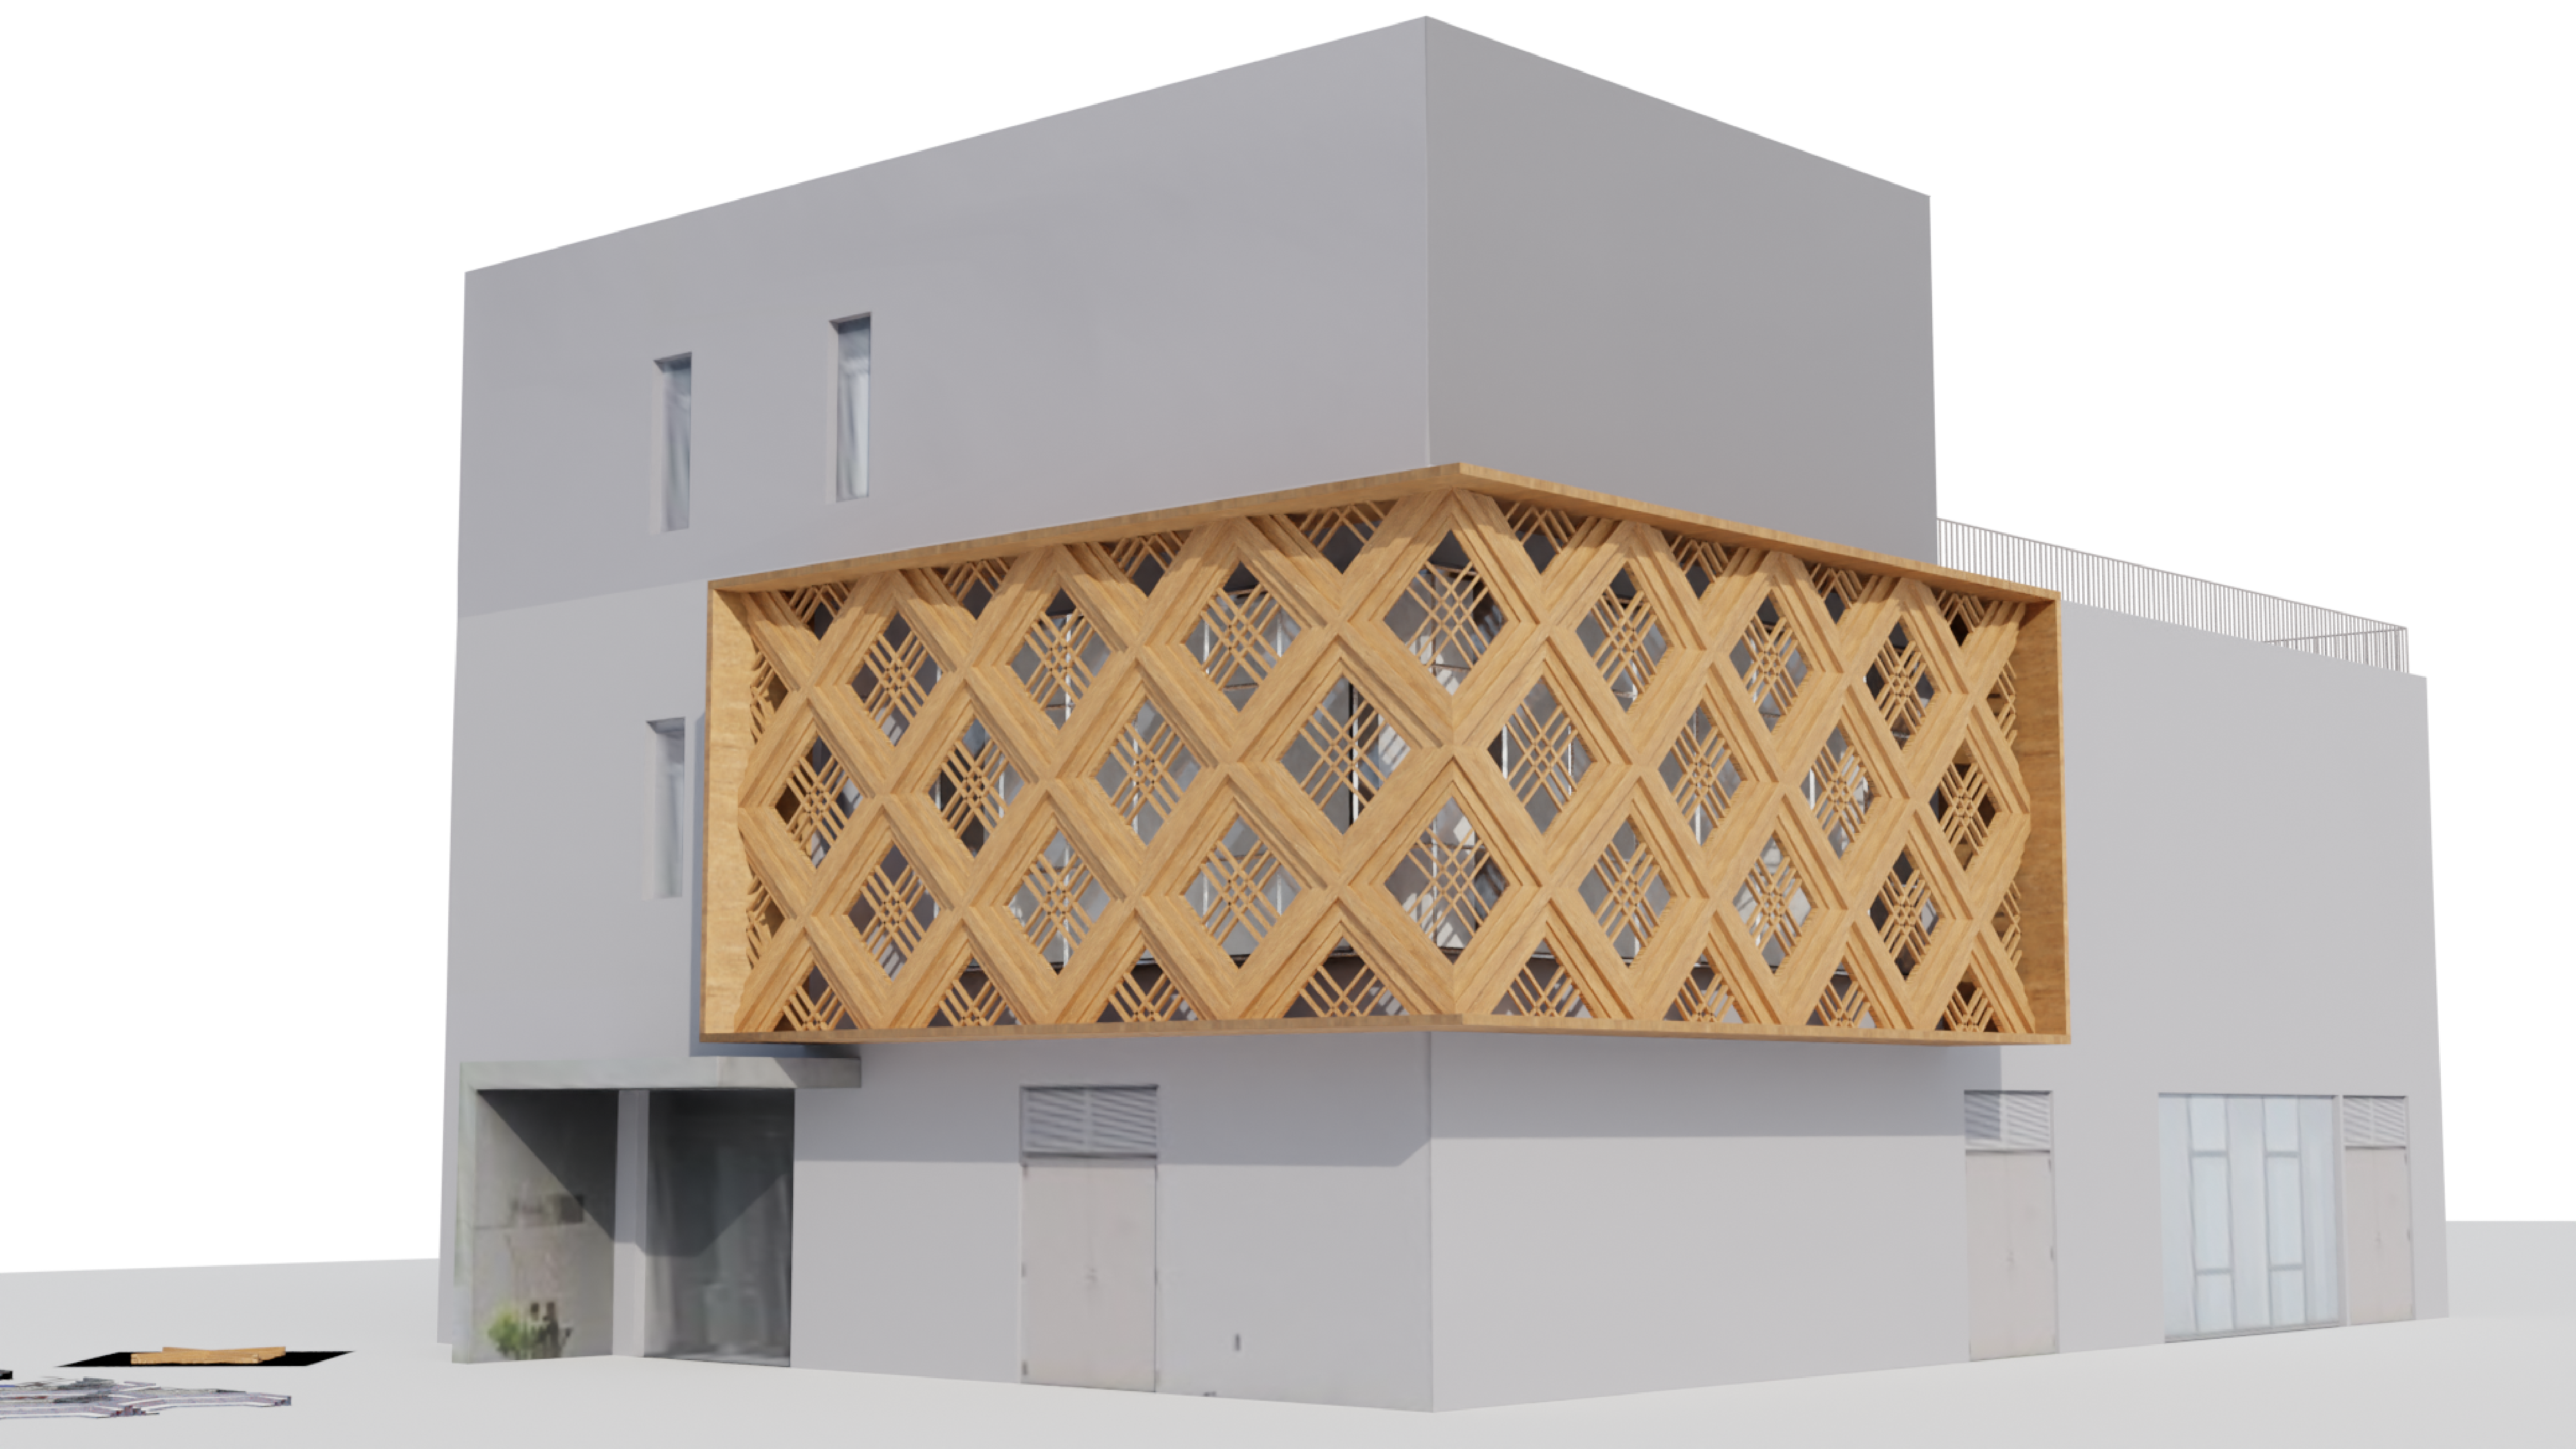
\includegraphics[width=1\linewidth]{Images/Pattern 1/0002}} &
              {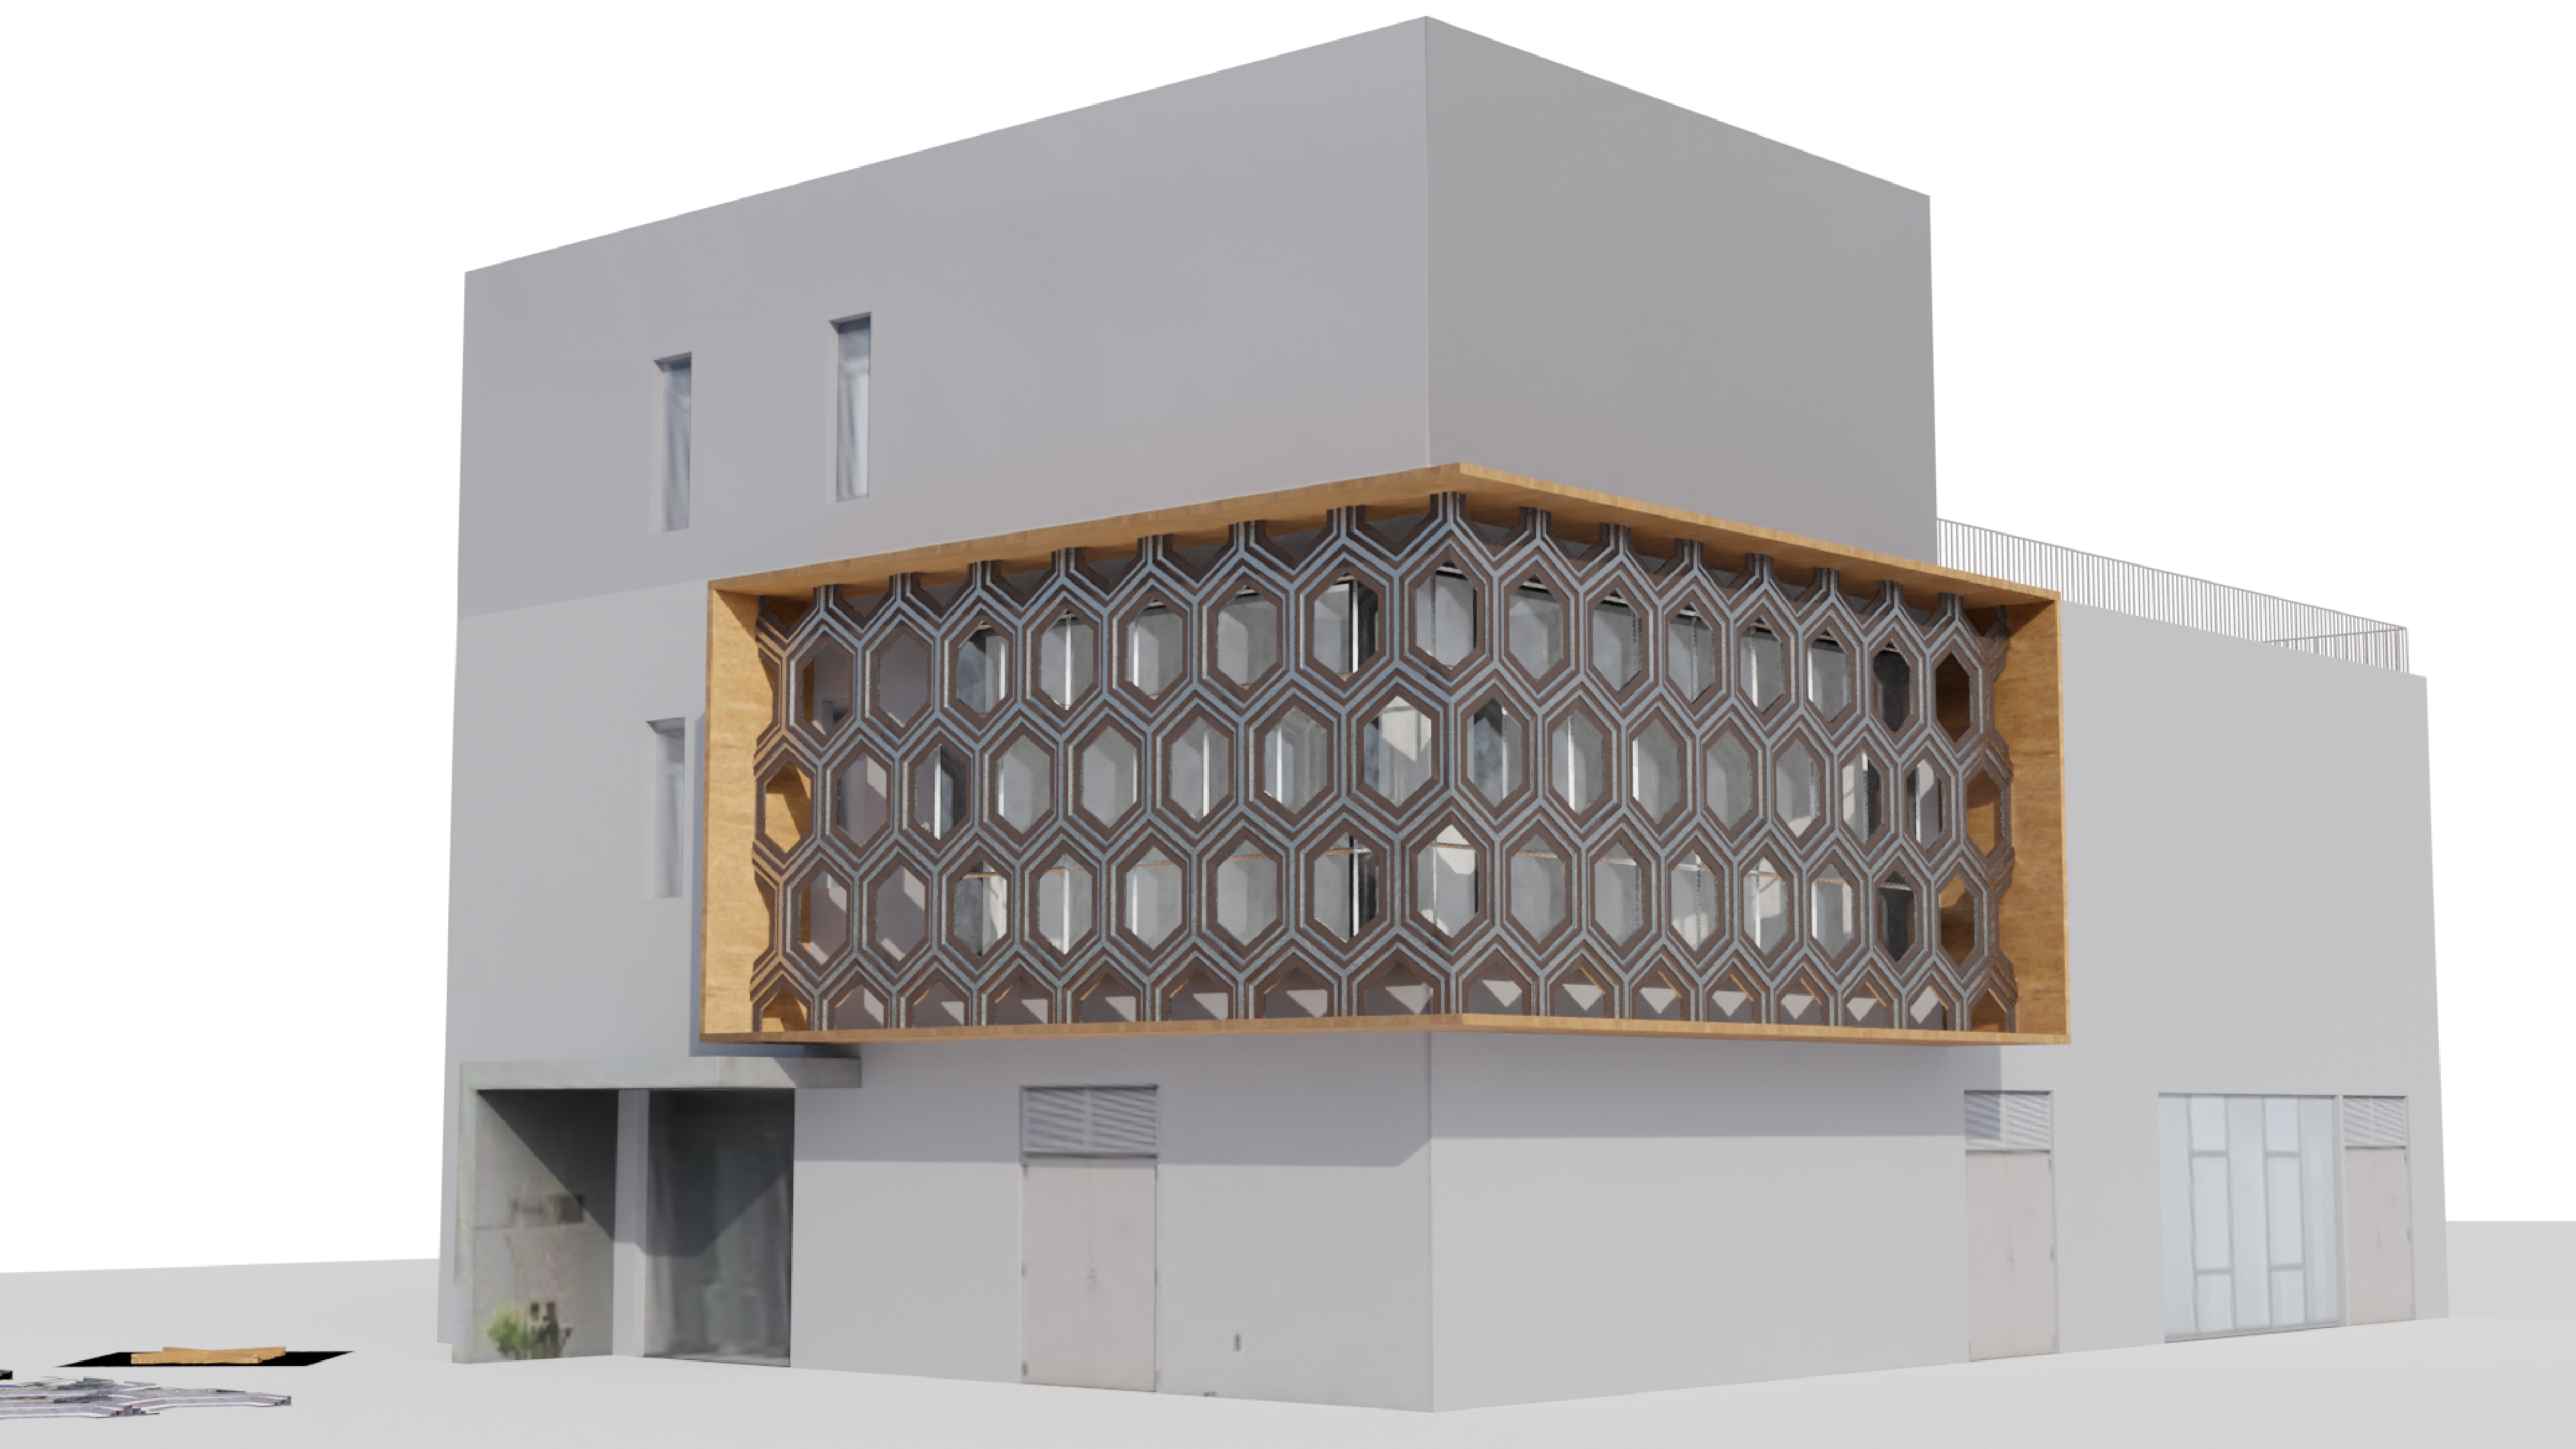
\includegraphics[width=1\linewidth]{Images/Pattern 2/0002}} &
              {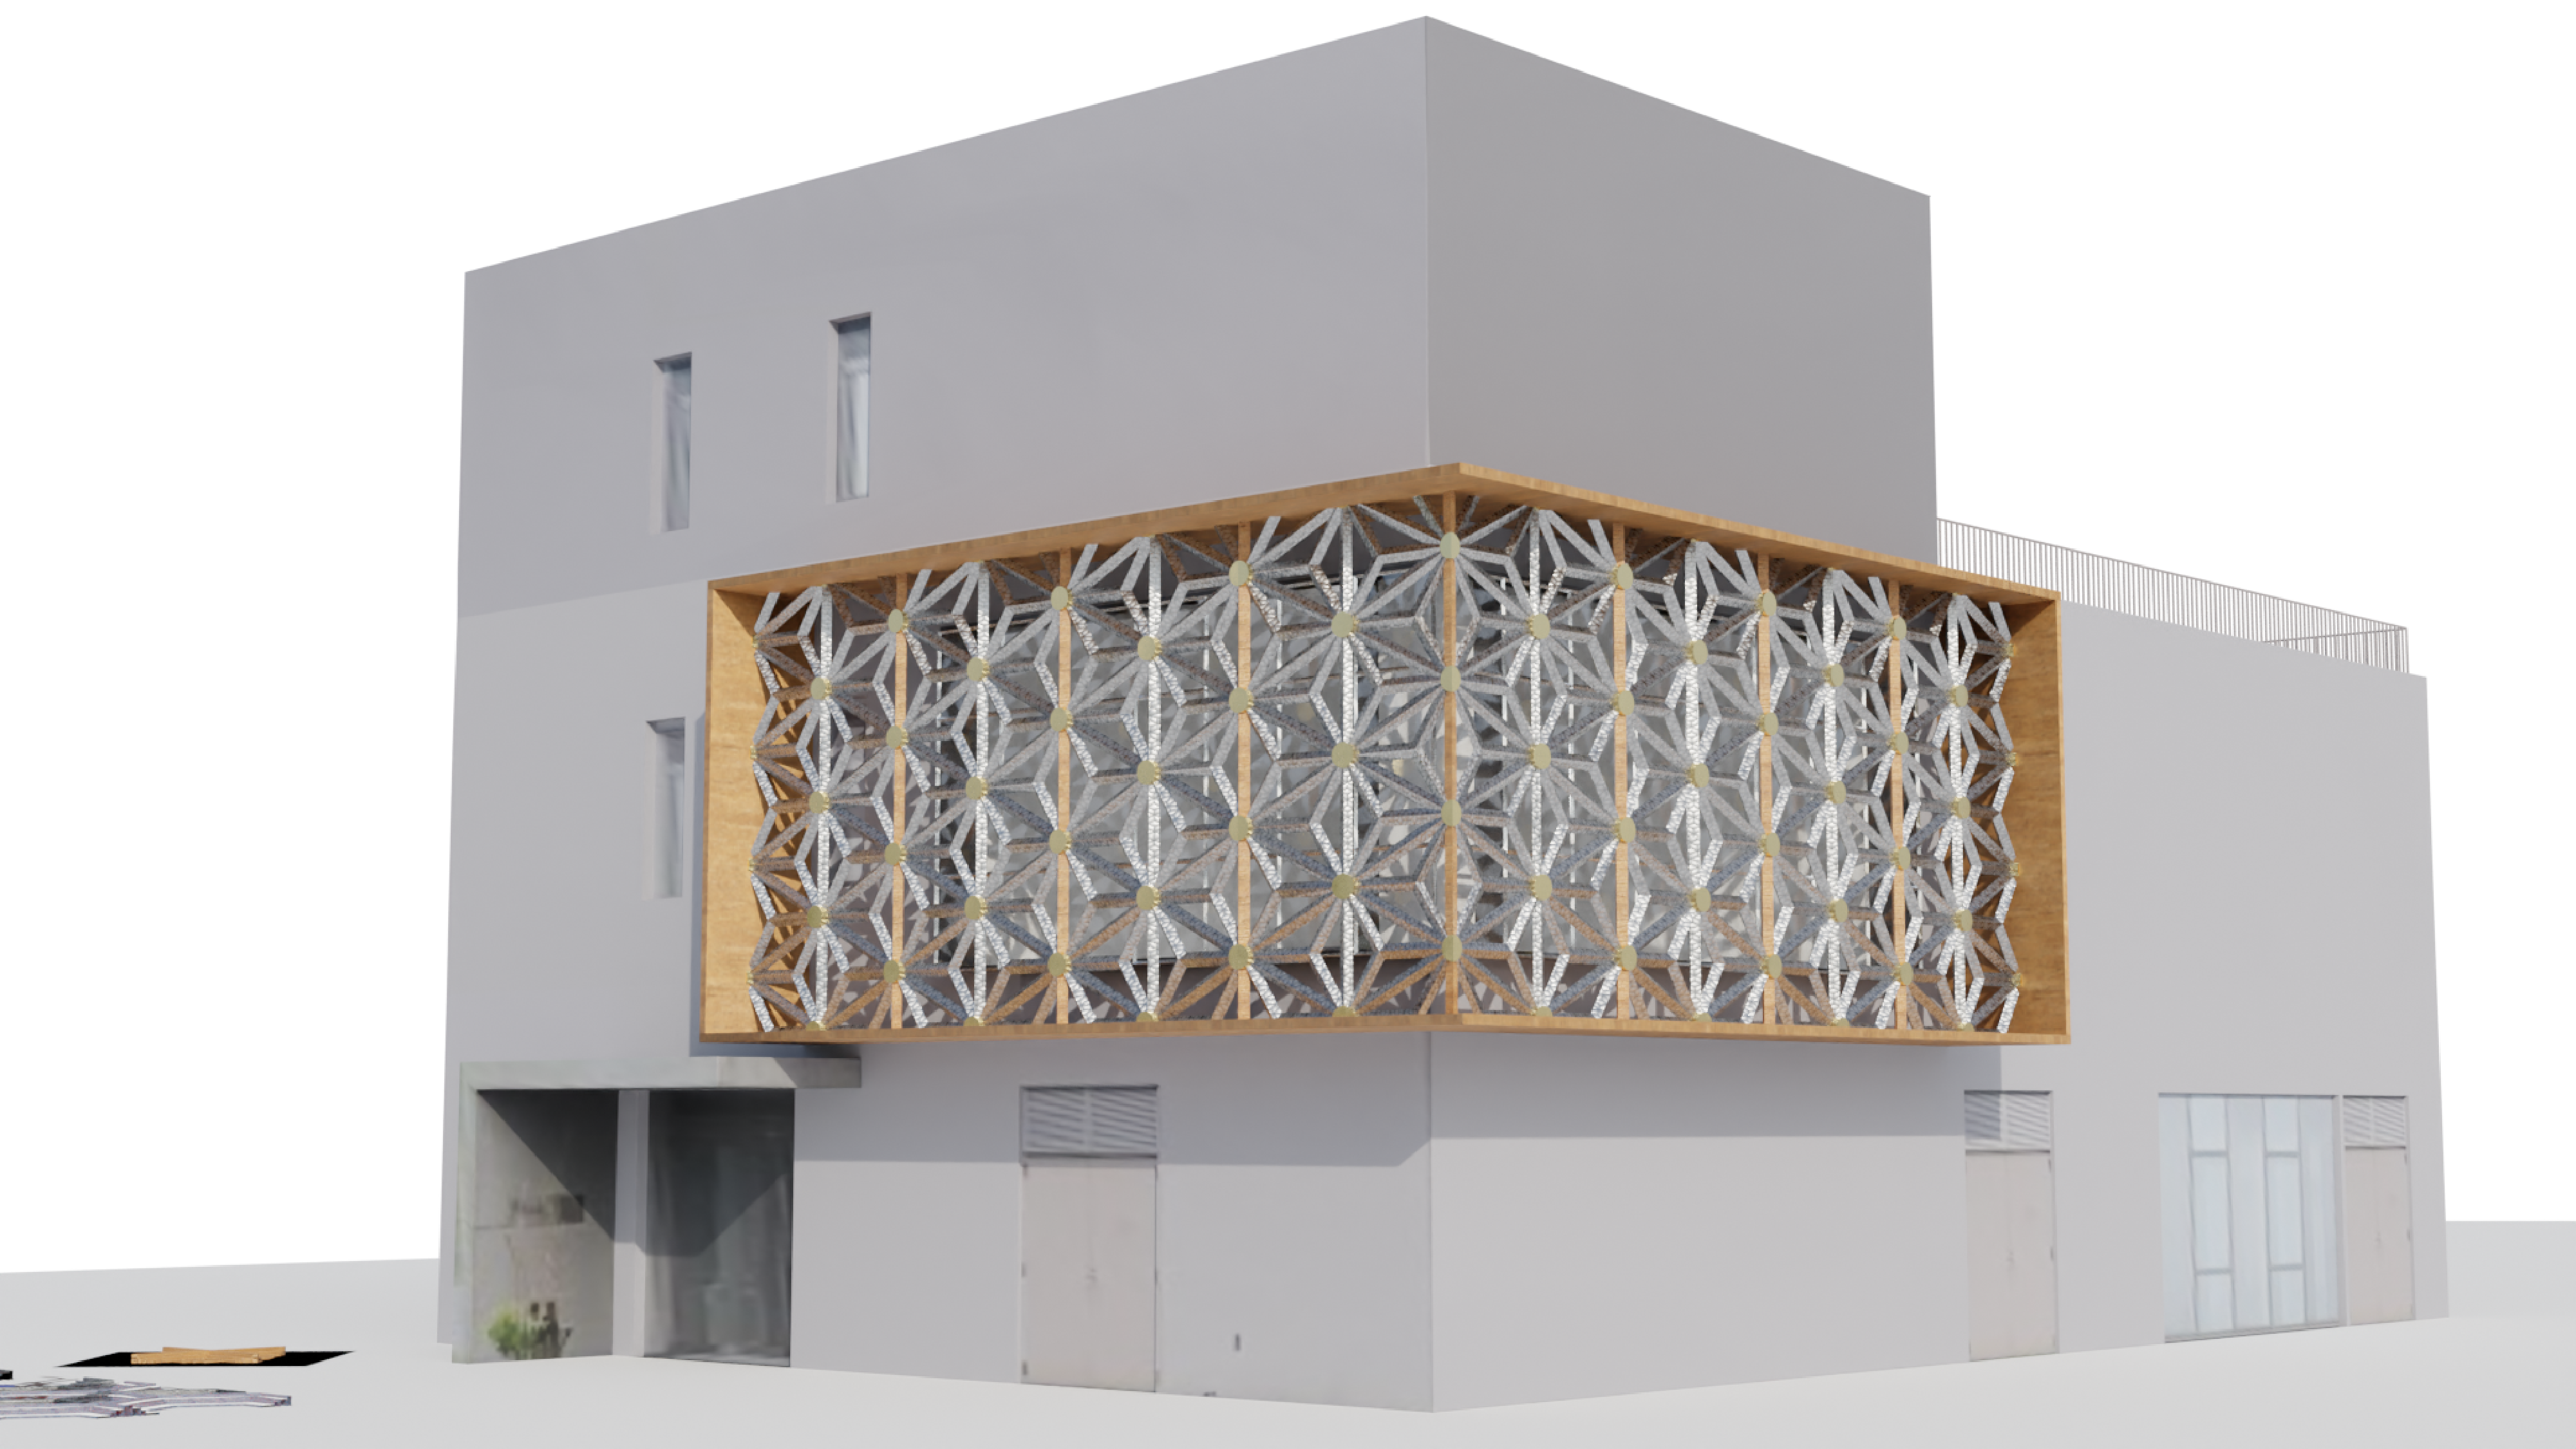
\includegraphics[width=1\linewidth]{Images/Pattern 3/0002}} \\
            \midrule
            \textit{Level 3} &  &  &
            \\
            {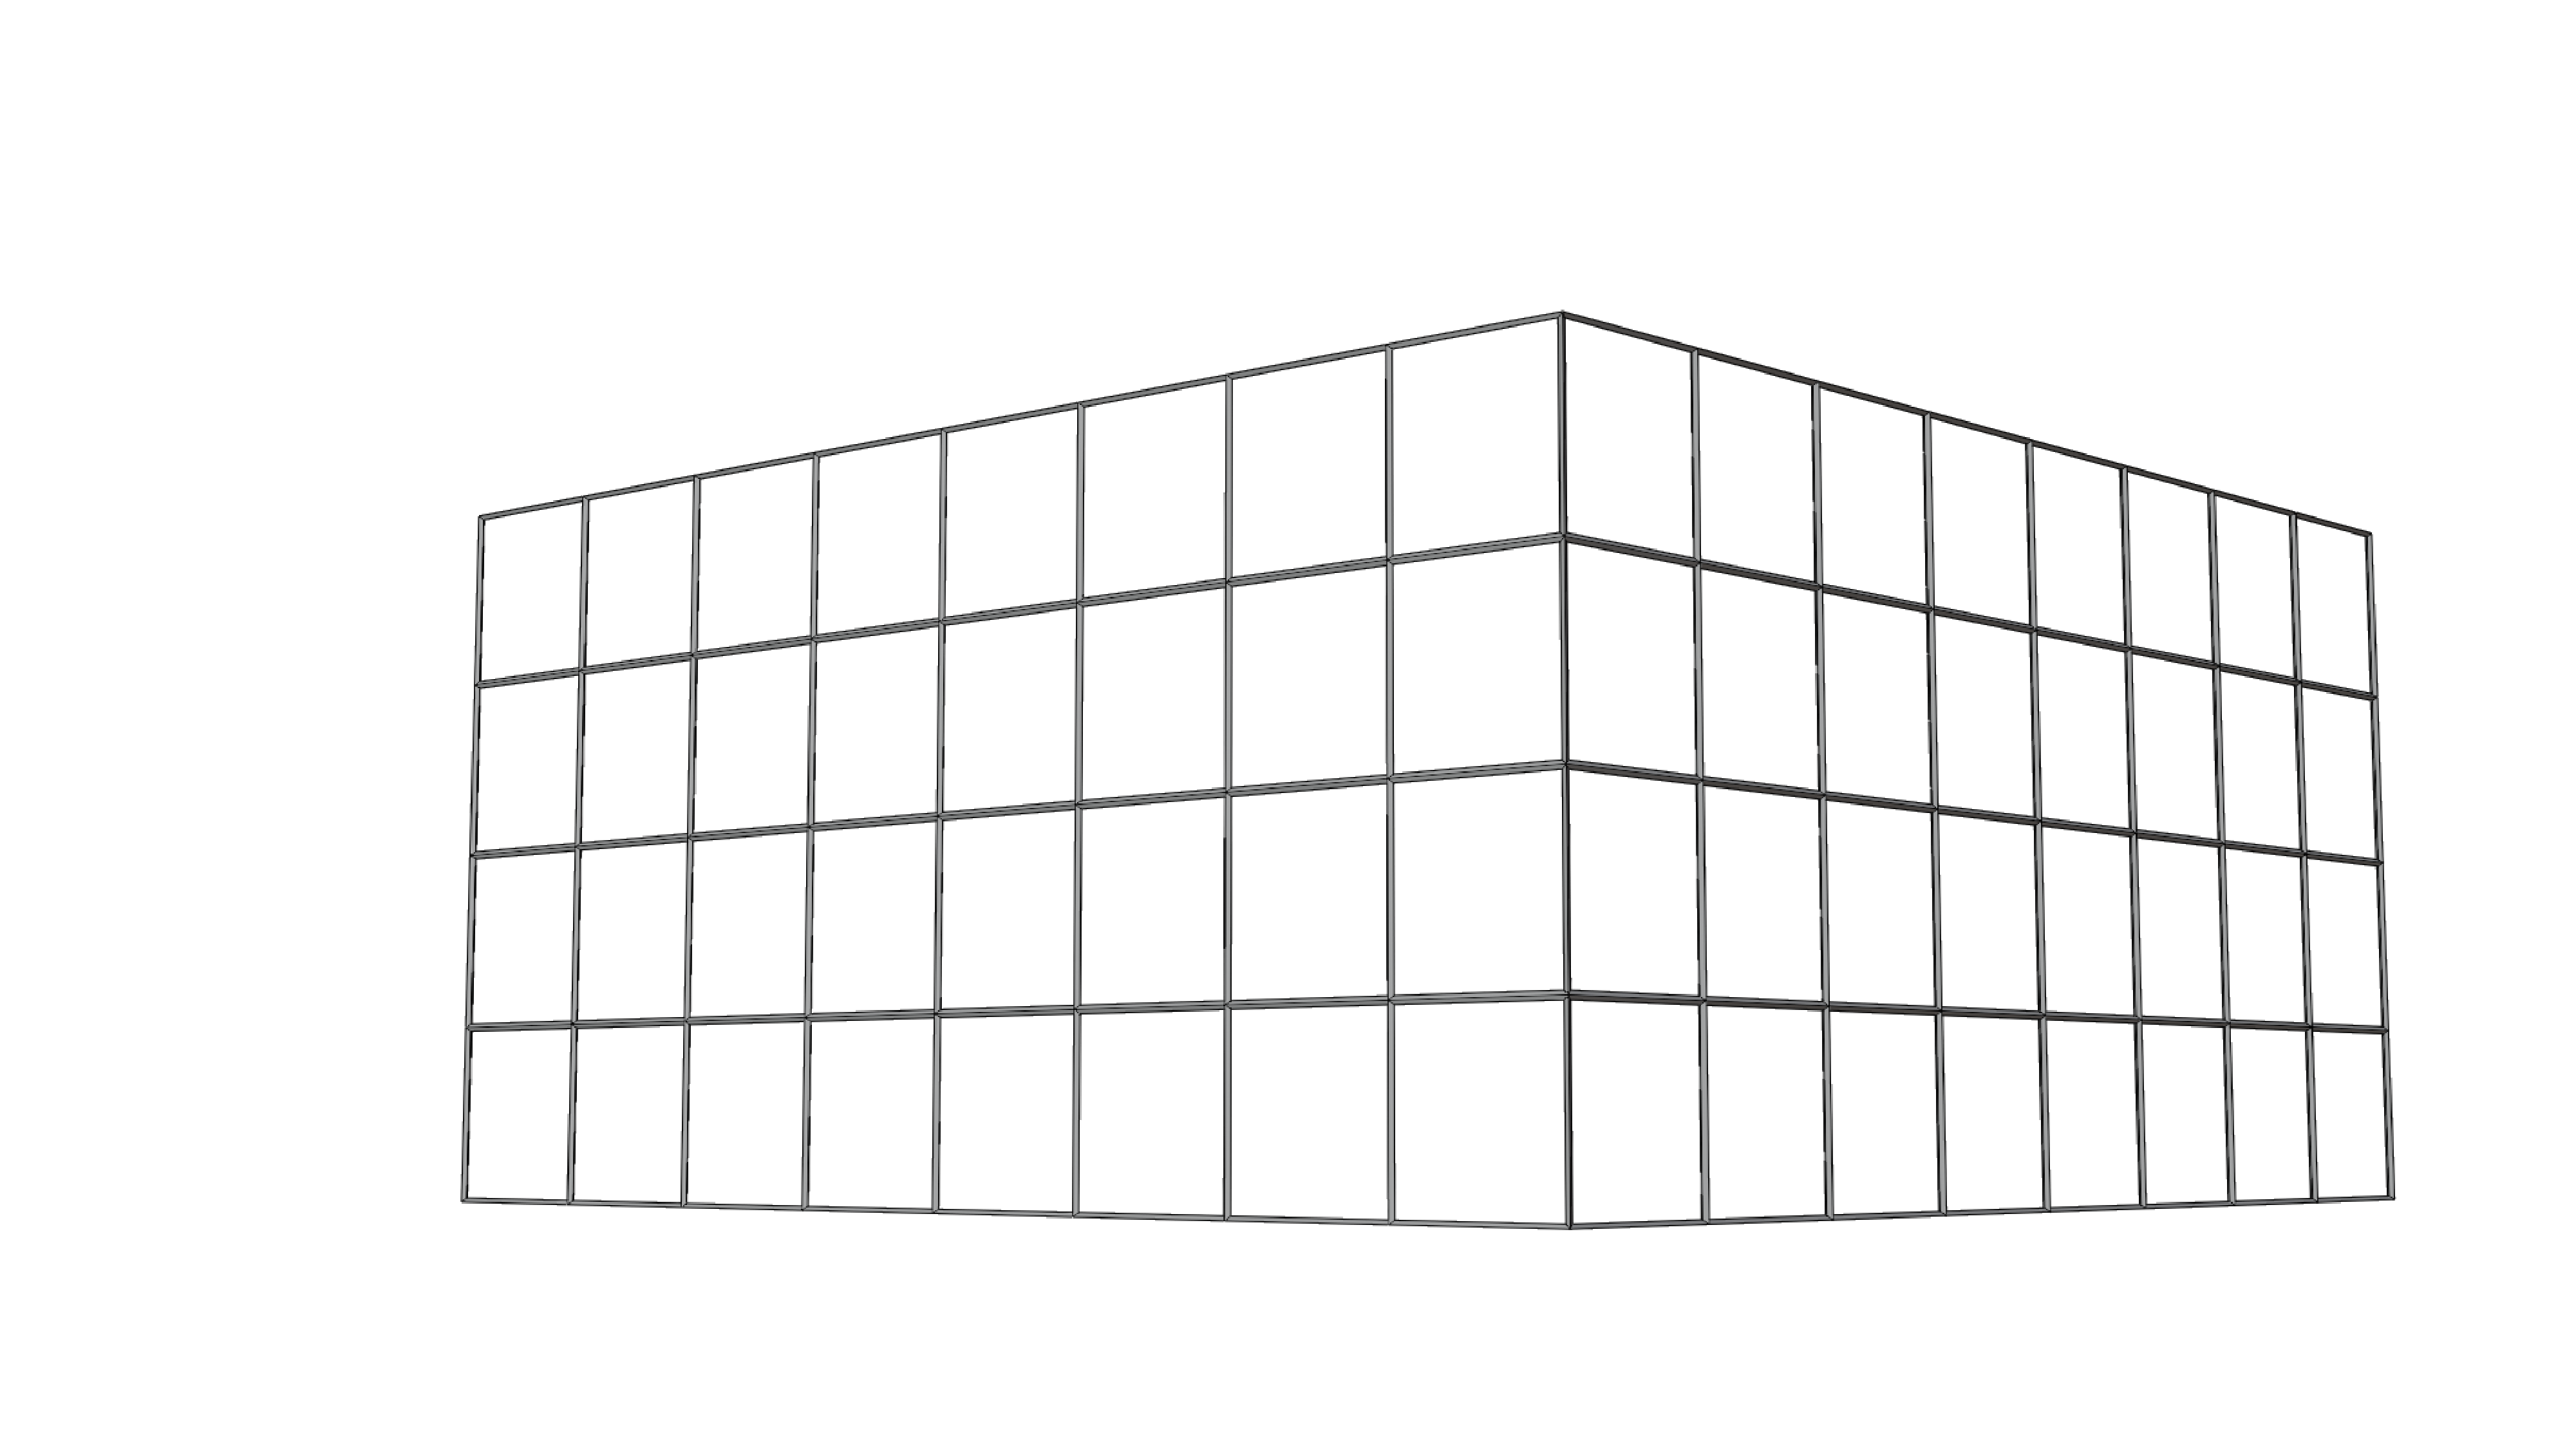
\includegraphics[width=1\linewidth]{Images/Wall 0/0003}} &
              {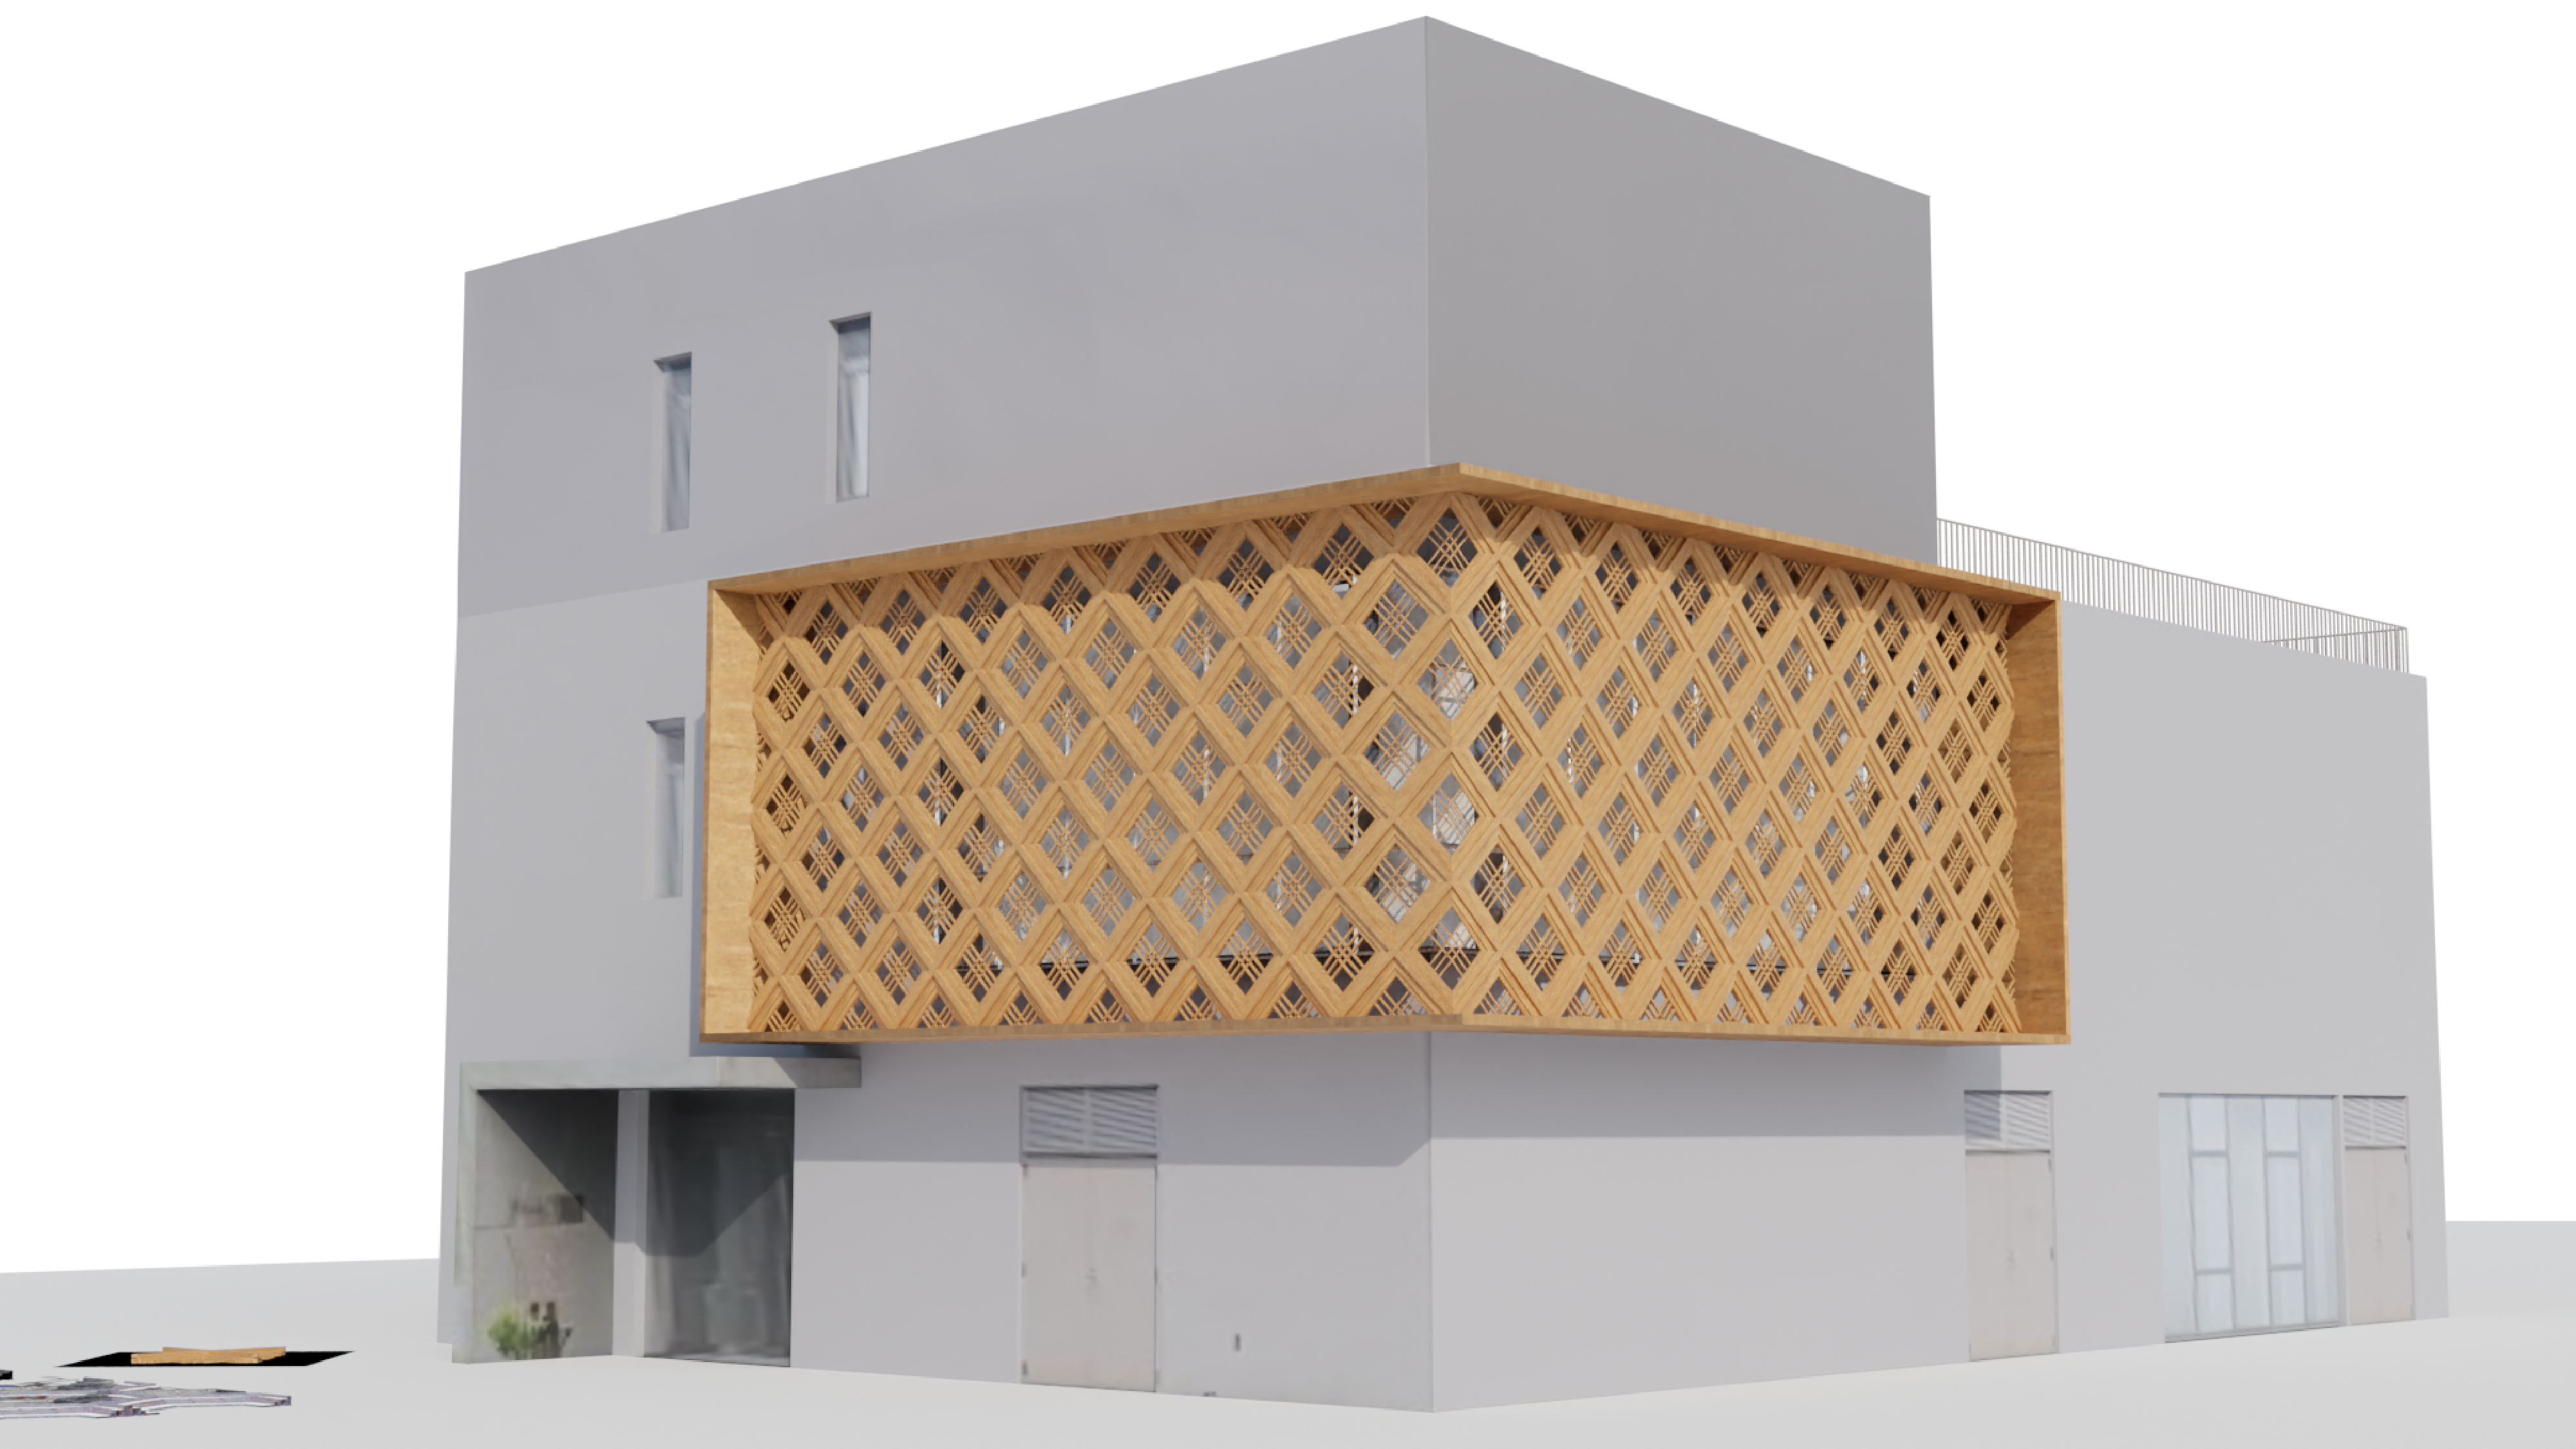
\includegraphics[width=1\linewidth]{Images/Pattern 1/0003}} &
              {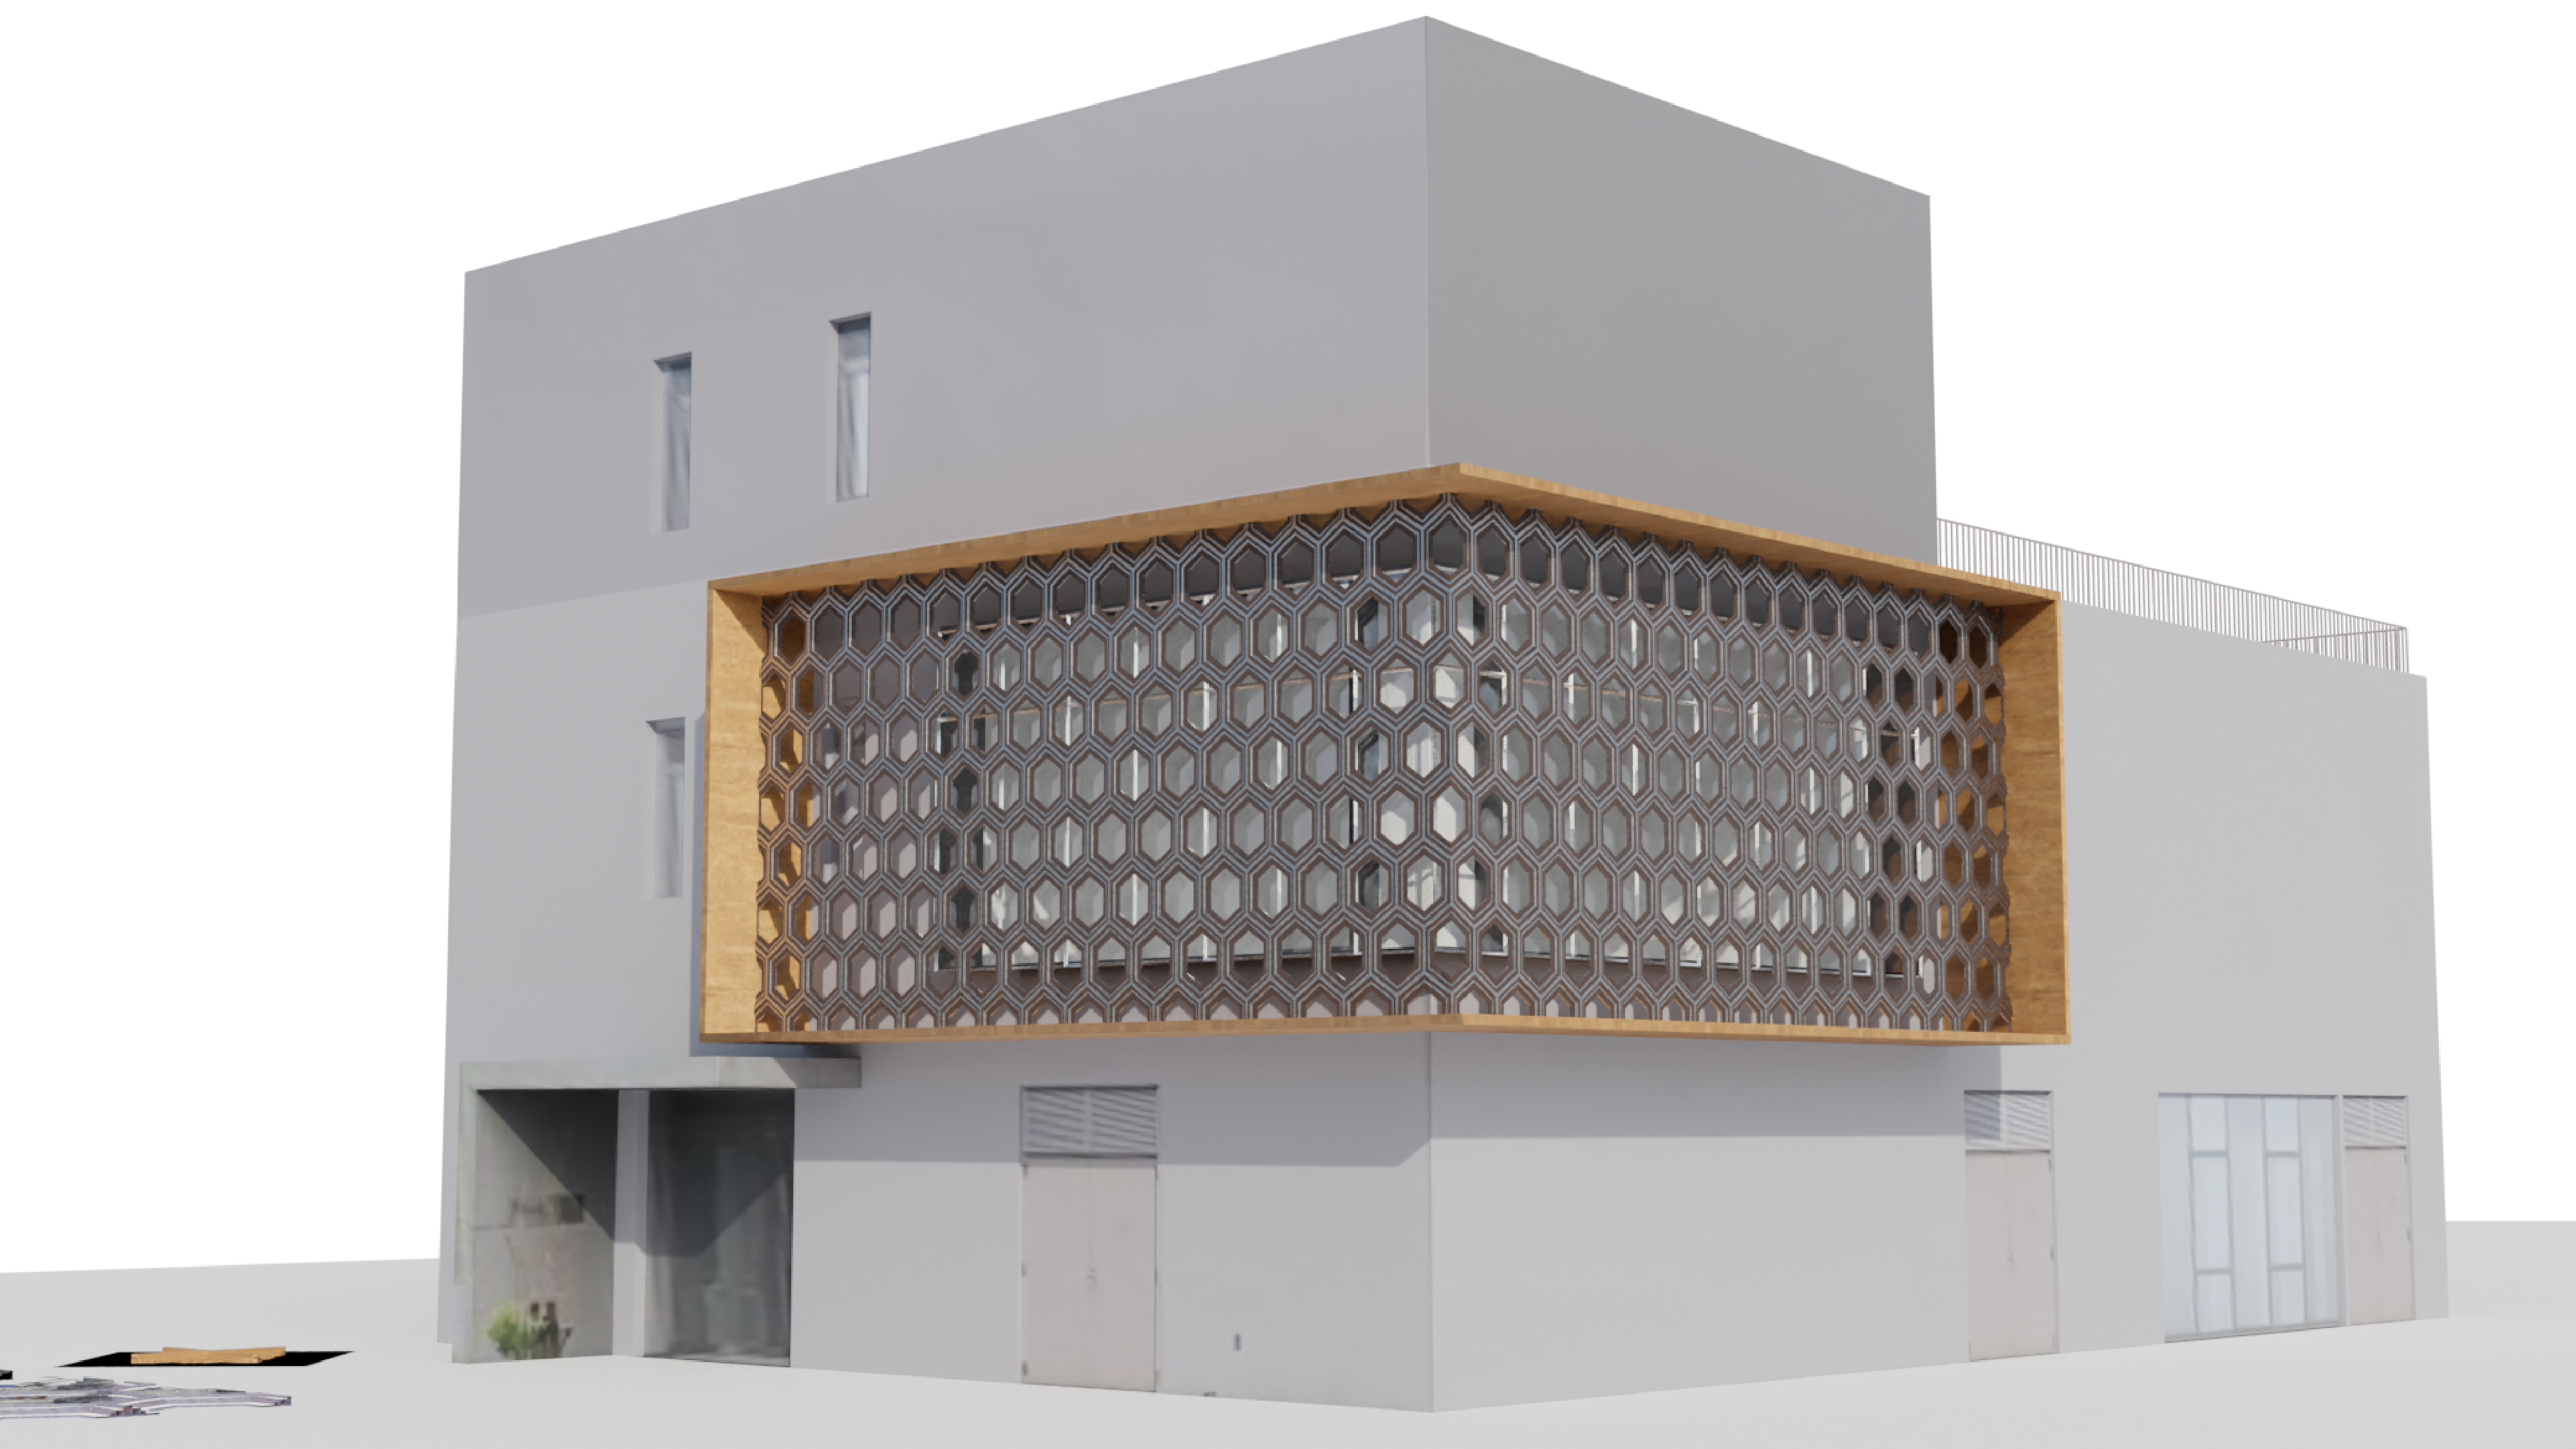
\includegraphics[width=1\linewidth]{Images/Pattern 2/0003}} &
              {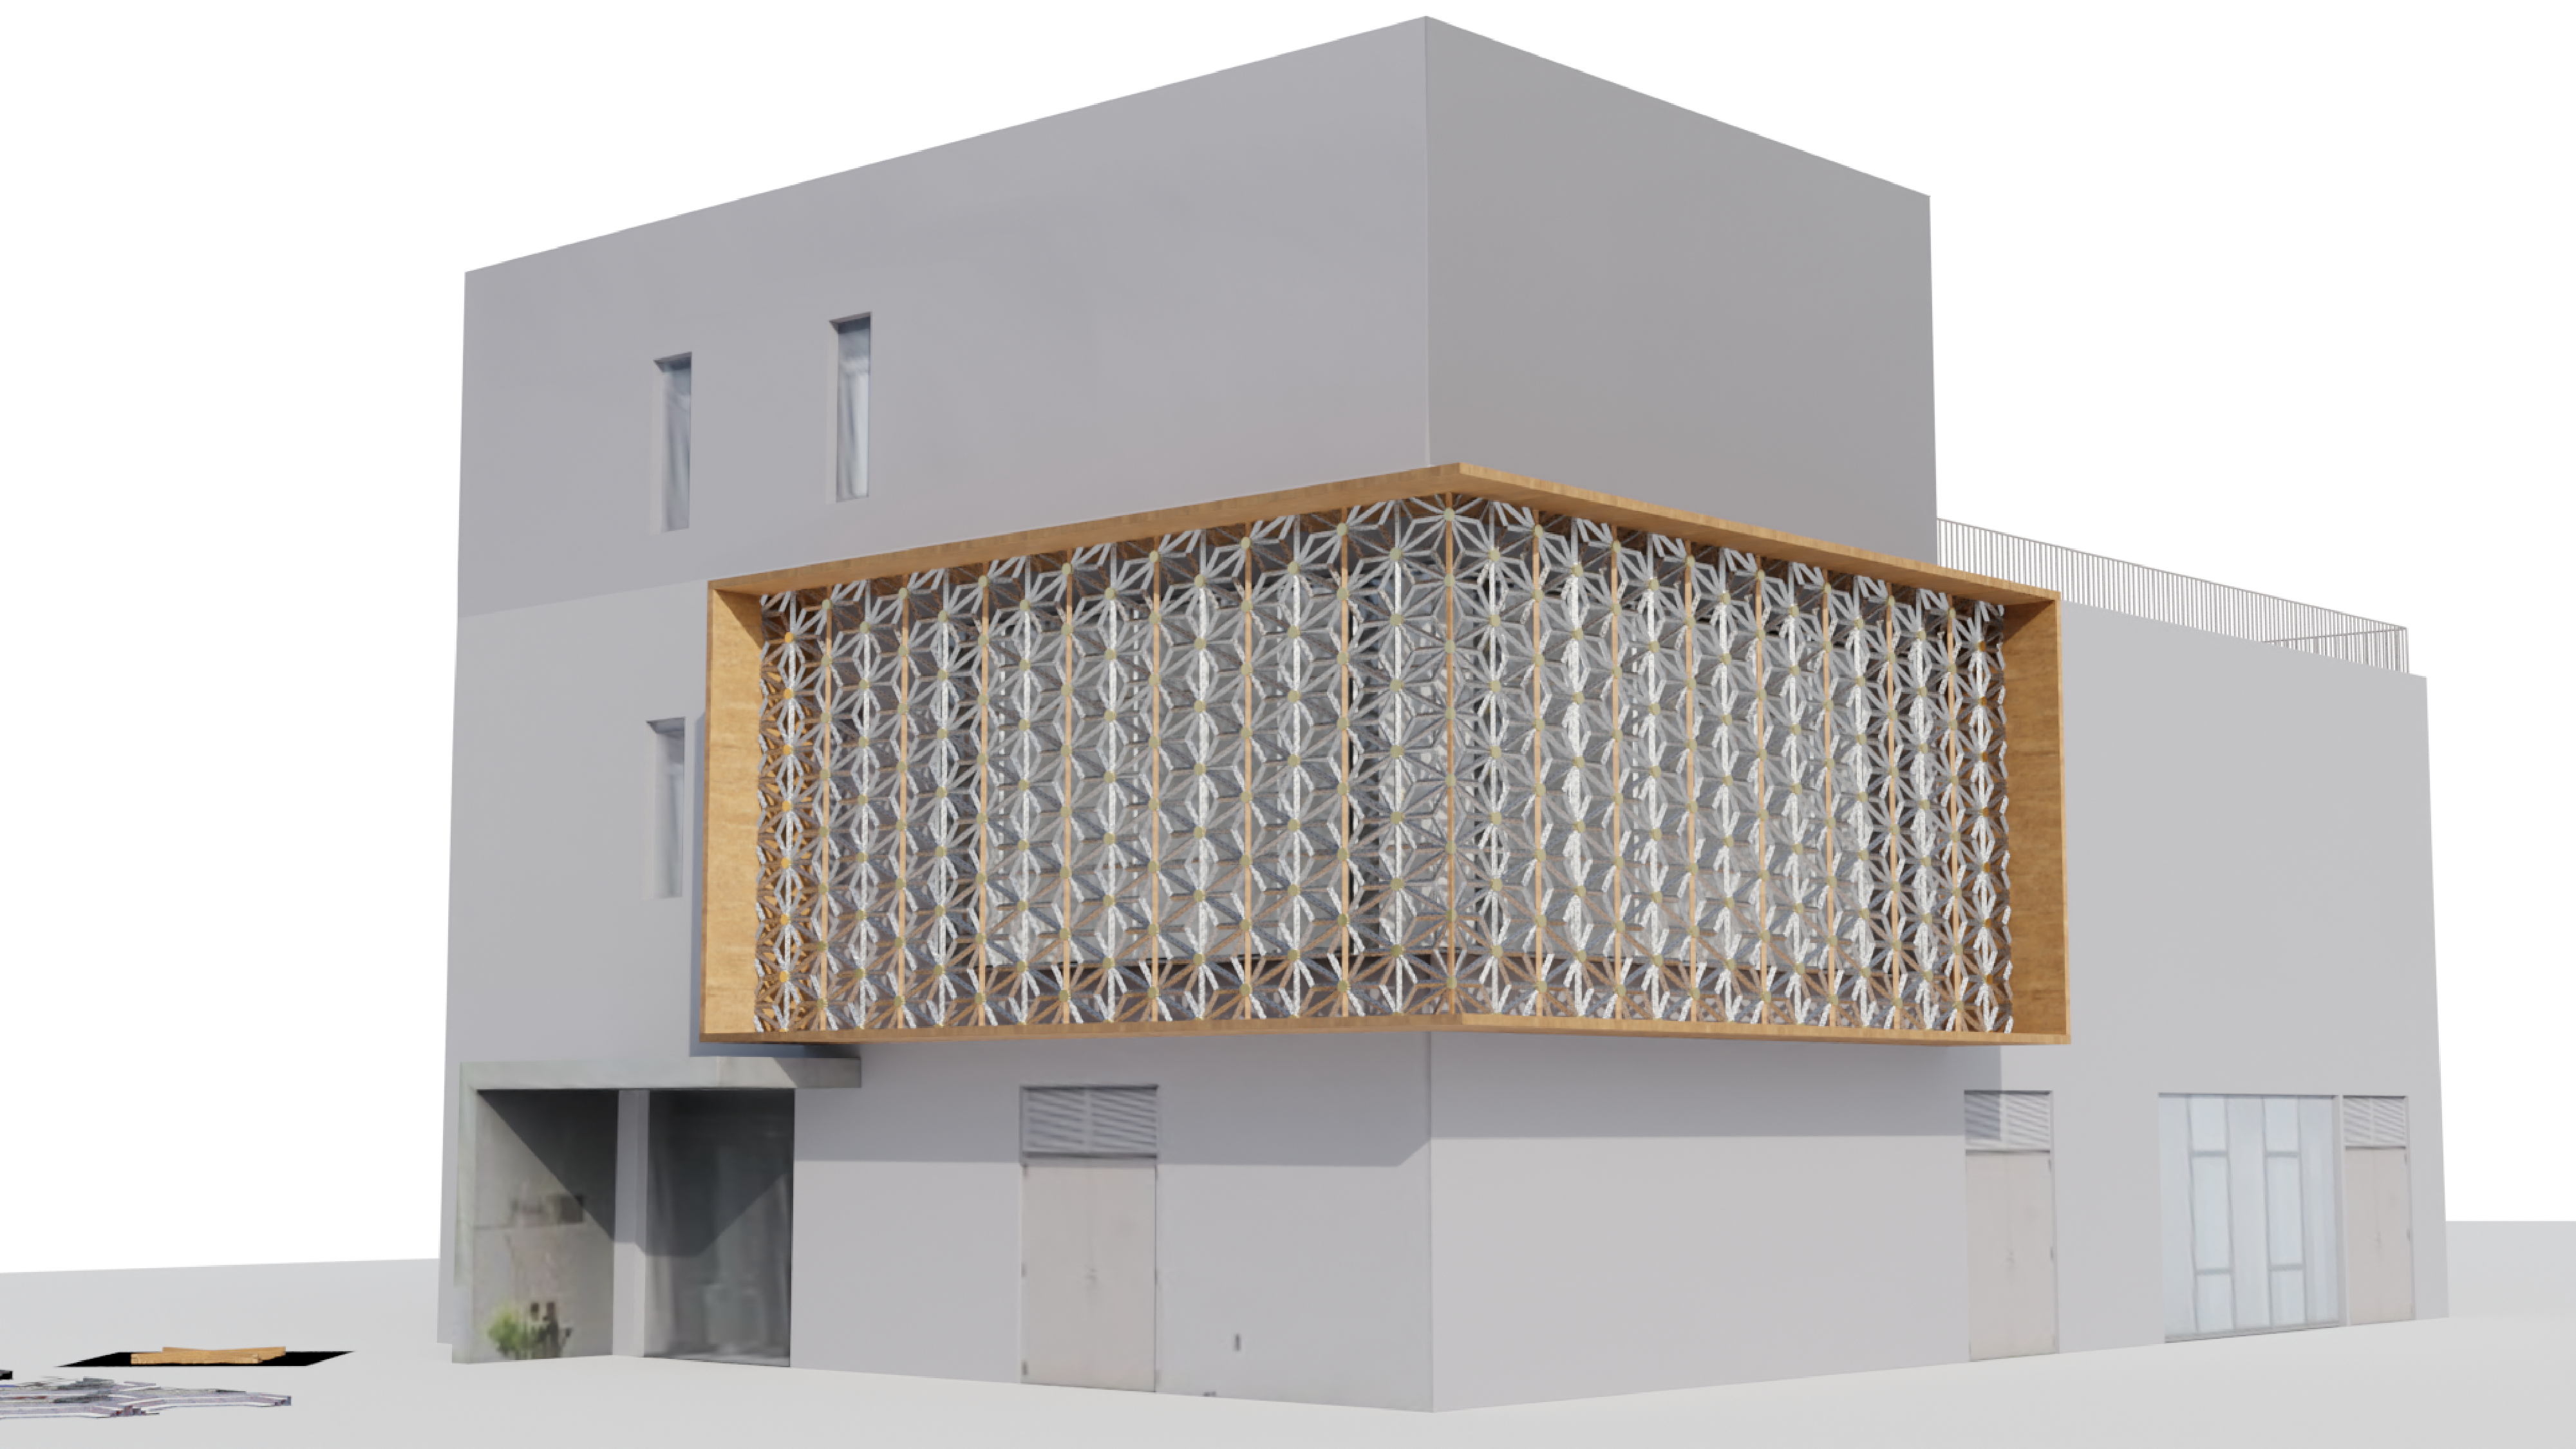
\includegraphics[width=1\linewidth]{Images/Pattern 3/0003}} \\
            \midrule
            \textit{Level 4} &  &  &
            \\
            {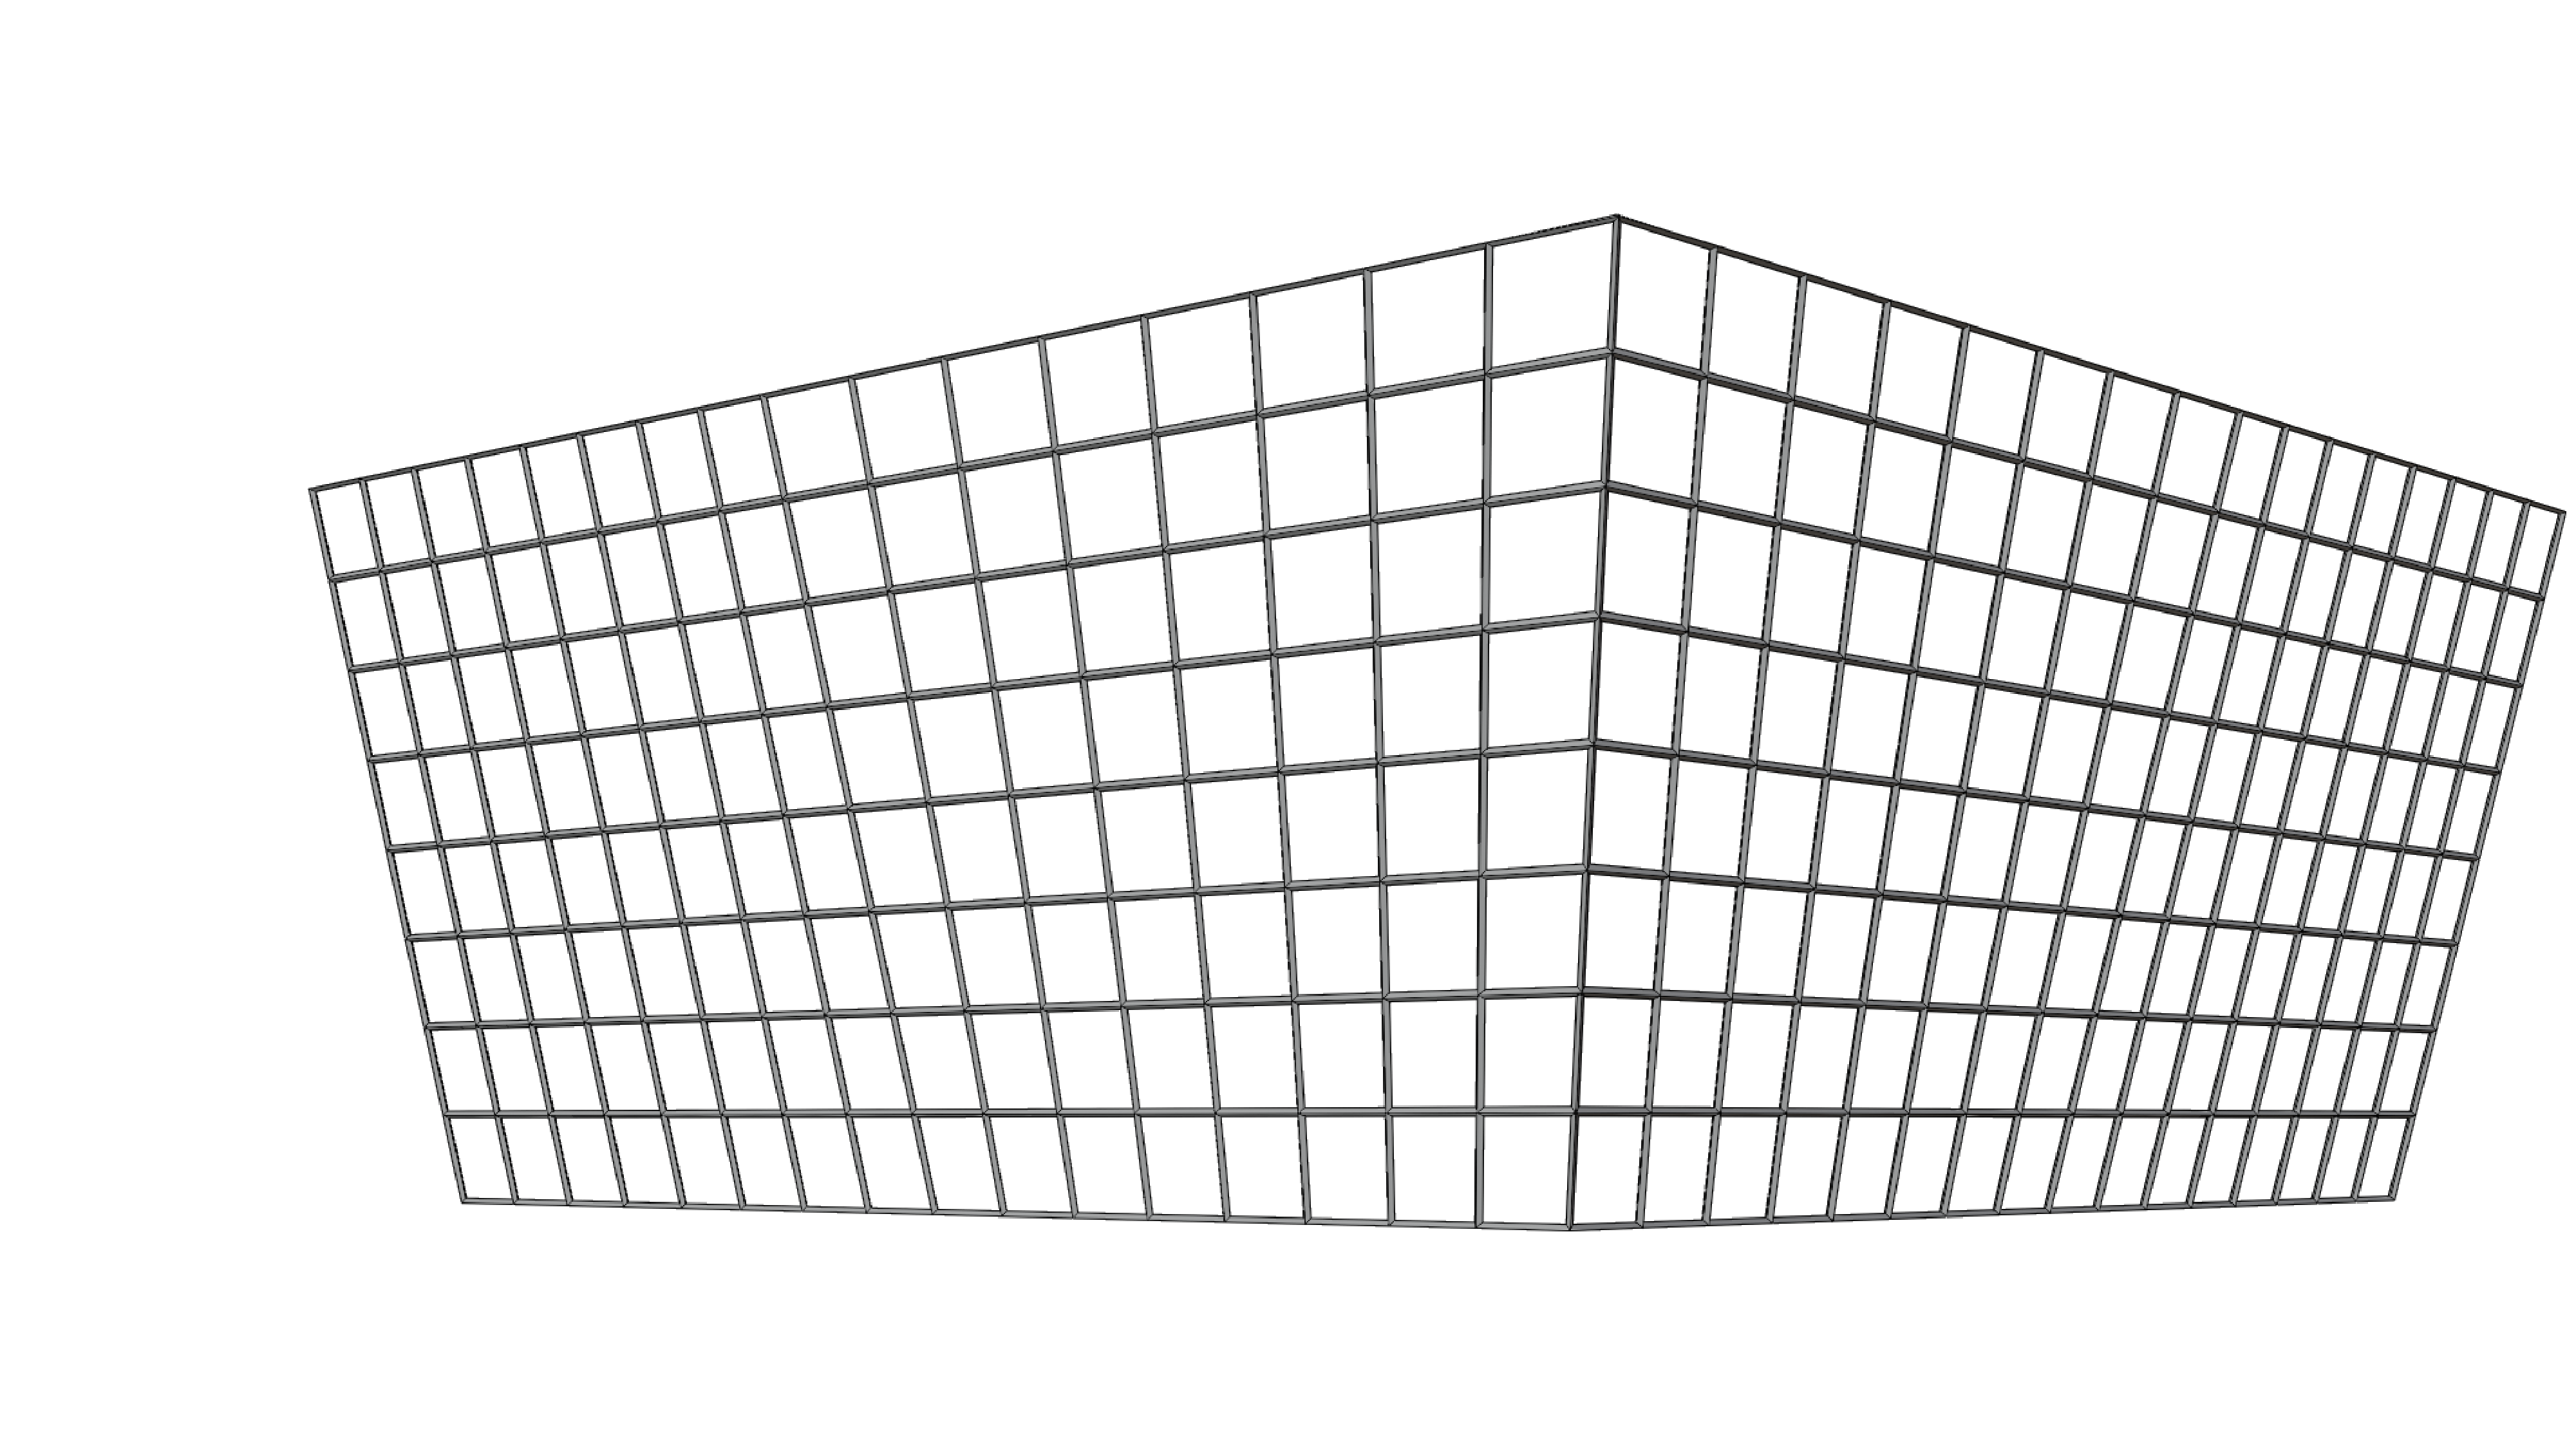
\includegraphics[width=1\linewidth]{Images/Wall 0/0004}} &
              {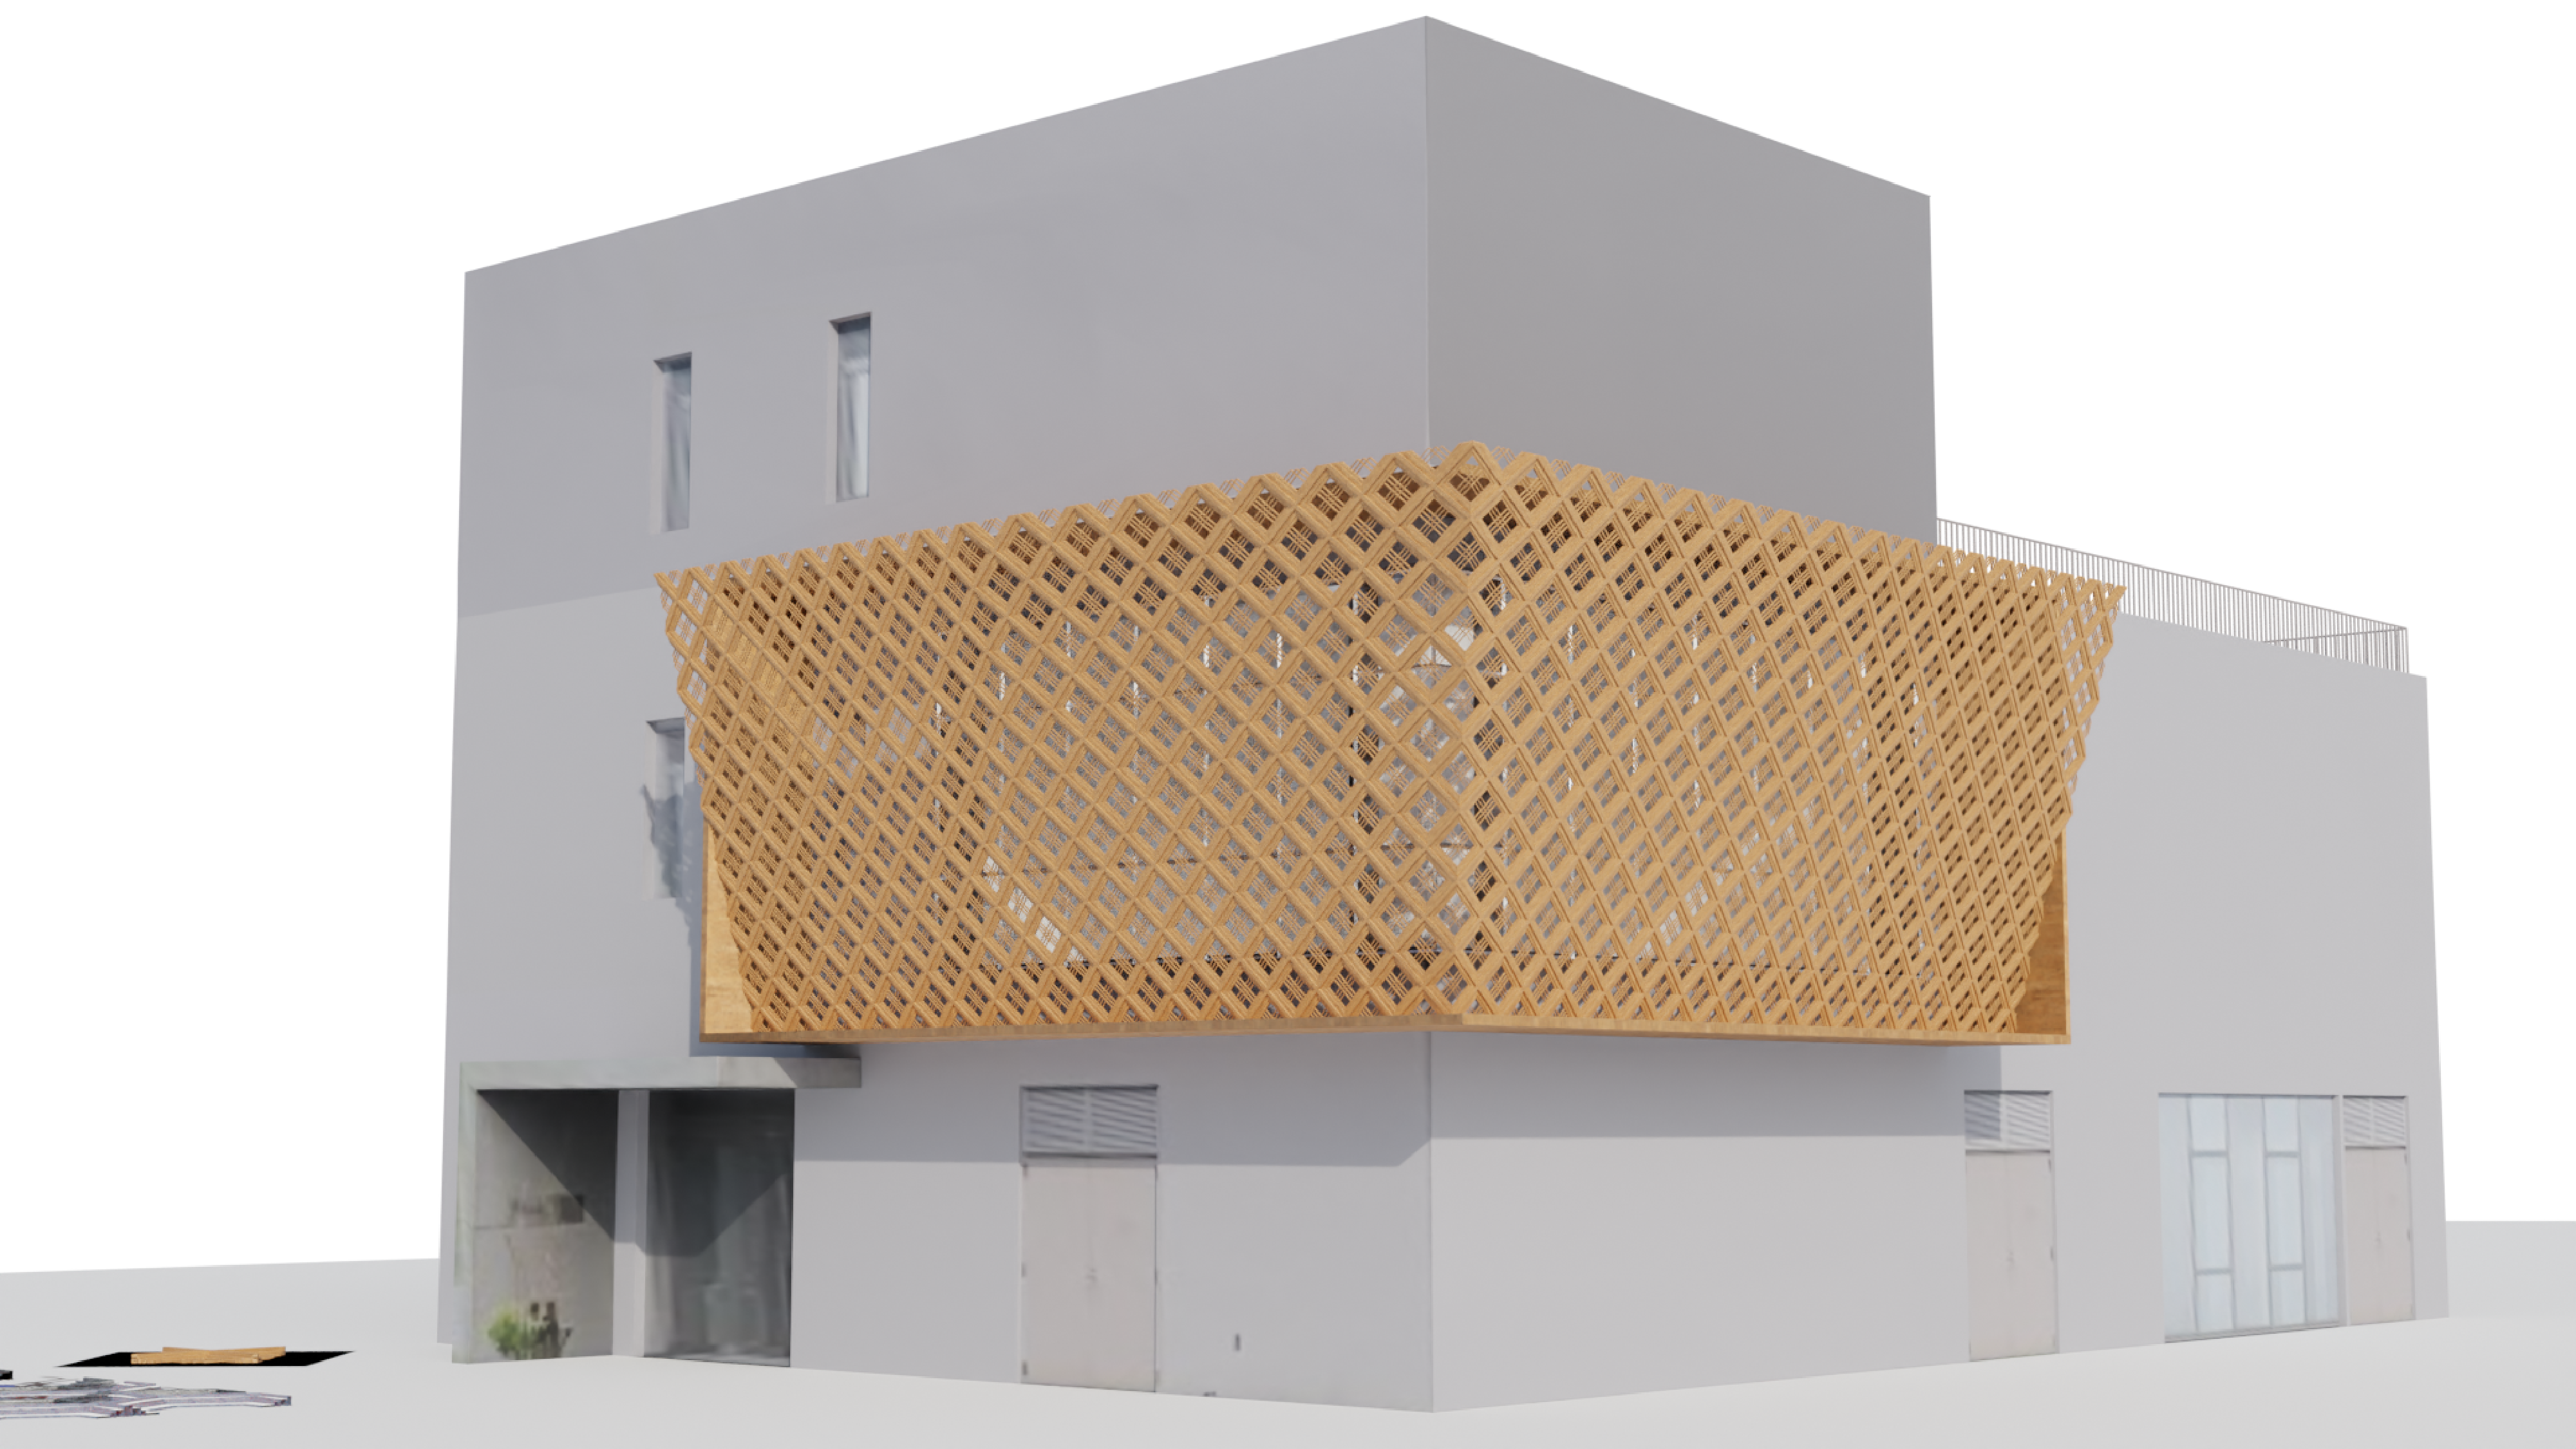
\includegraphics[width=1\linewidth]{Images/Pattern 1/0004}} &
              {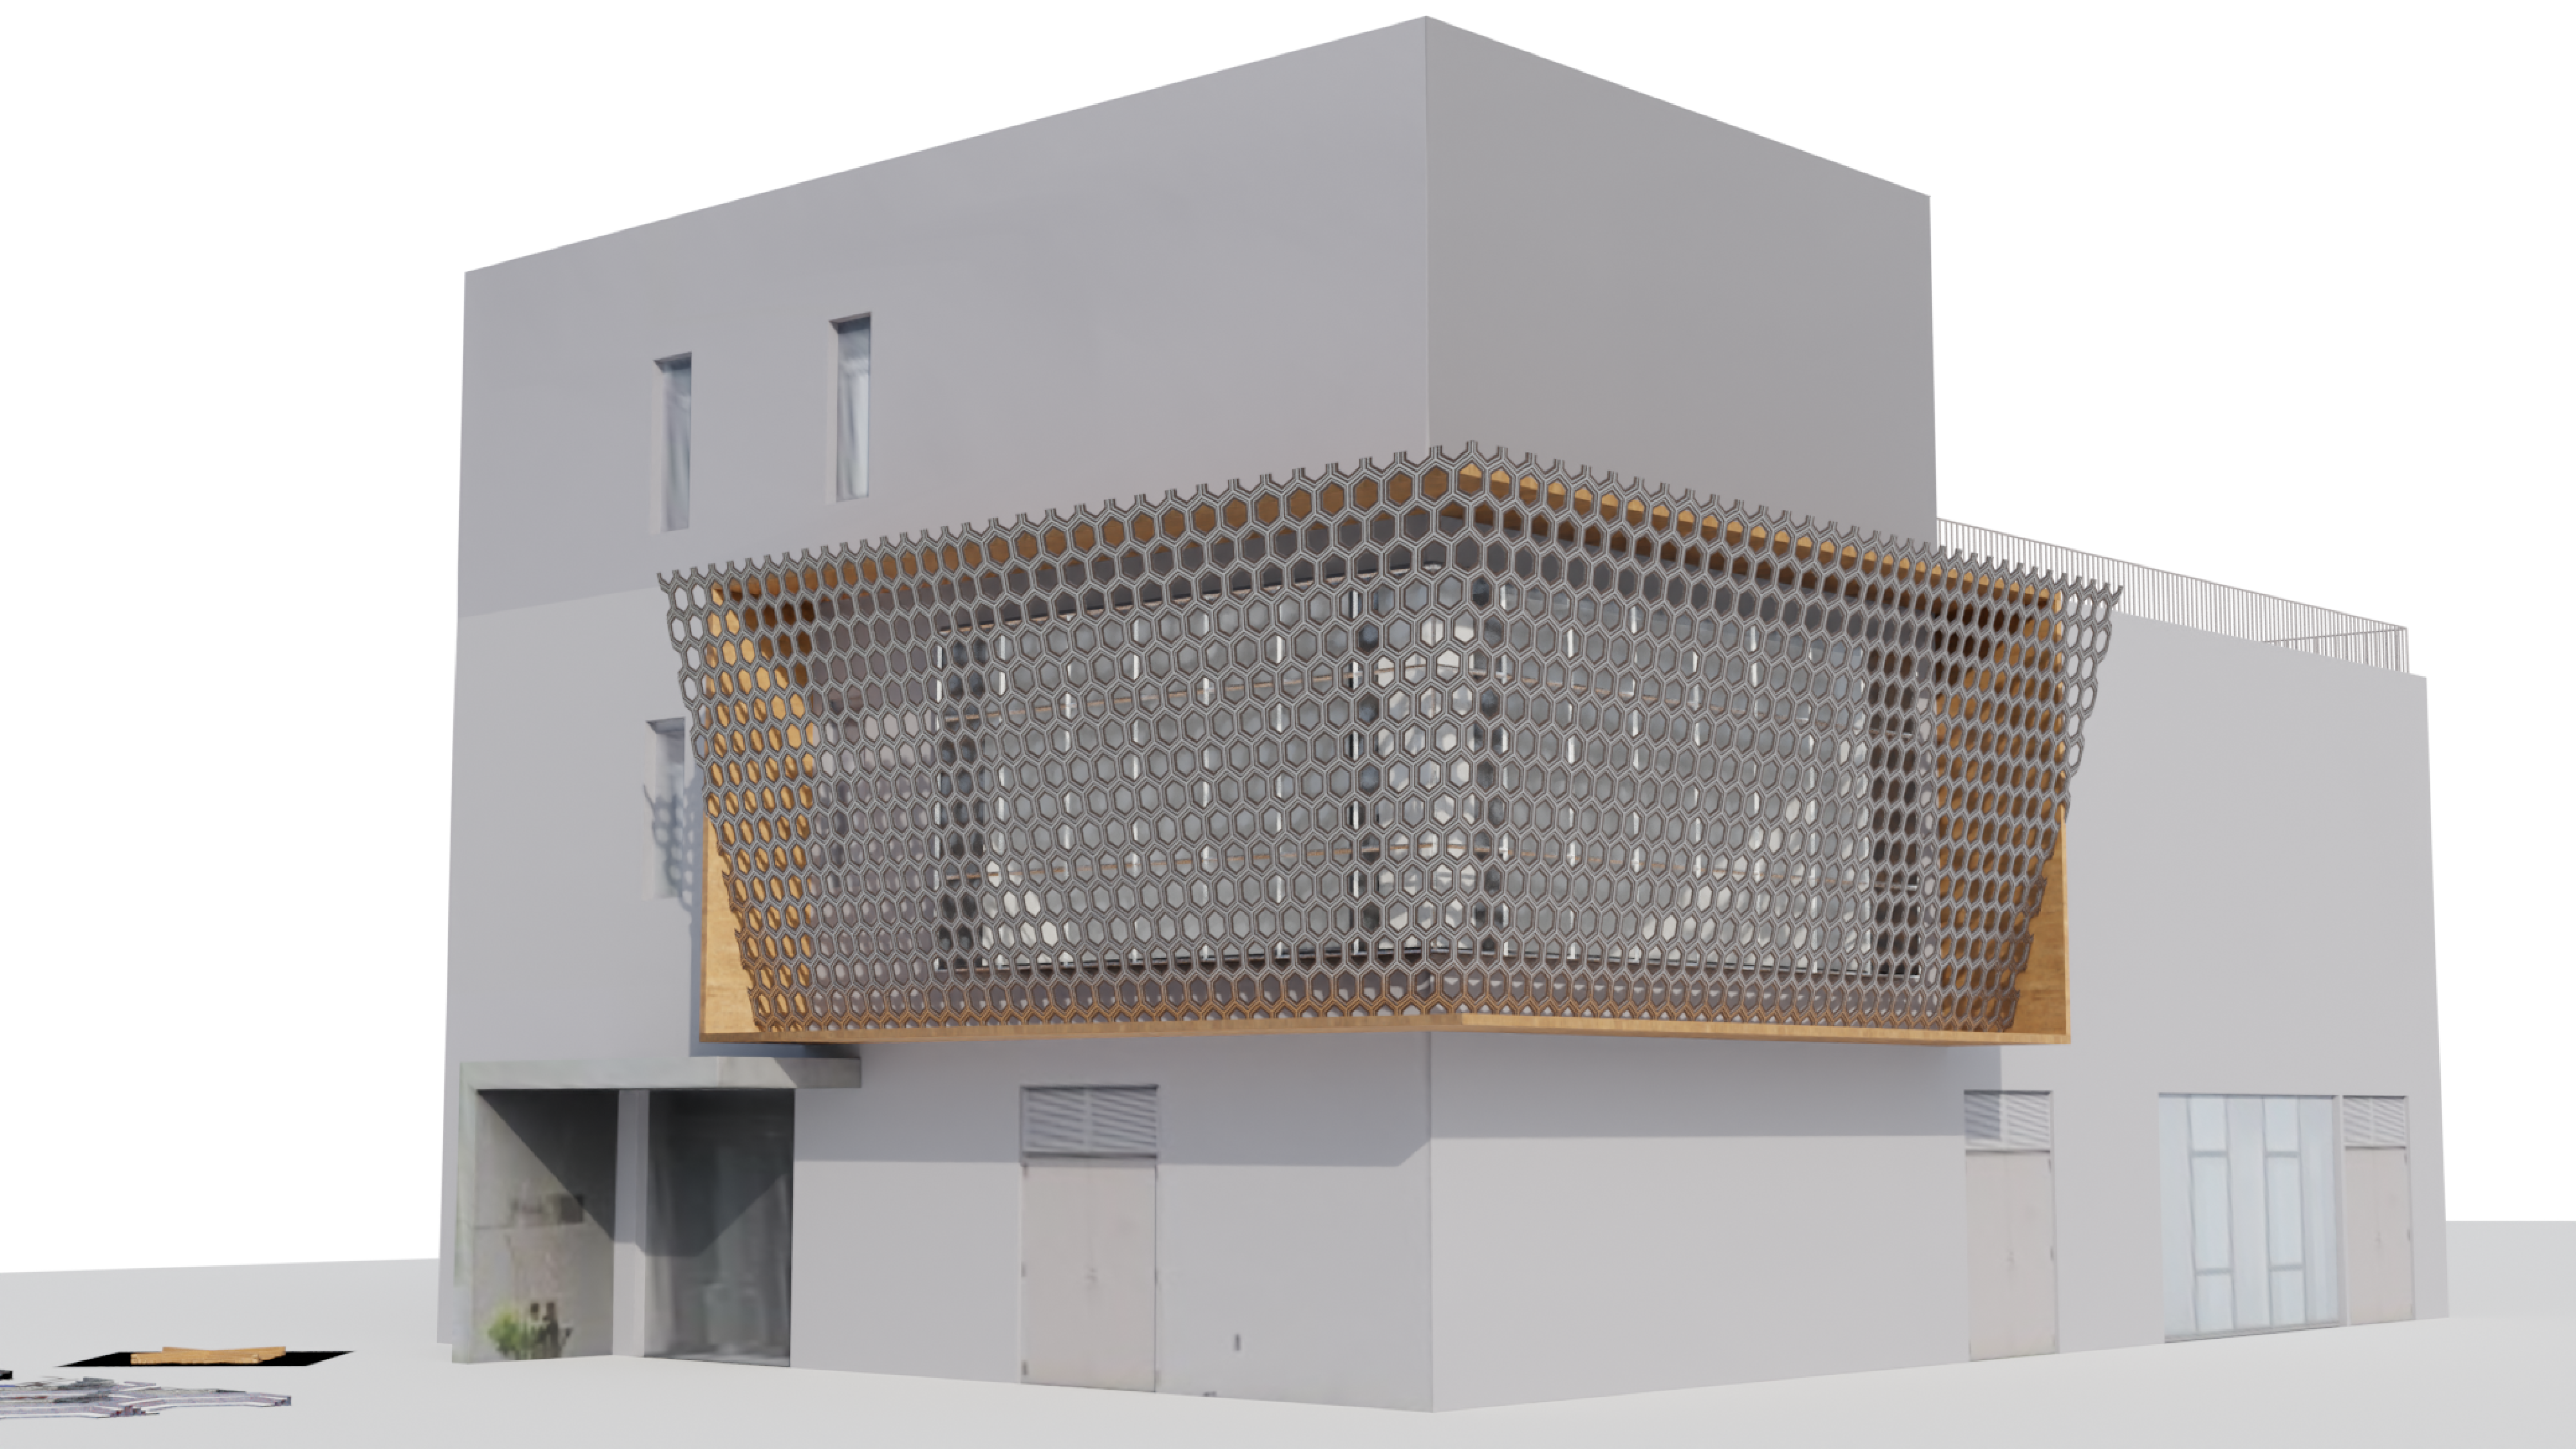
\includegraphics[width=1\linewidth]{Images/Pattern 2/0004}} &
              {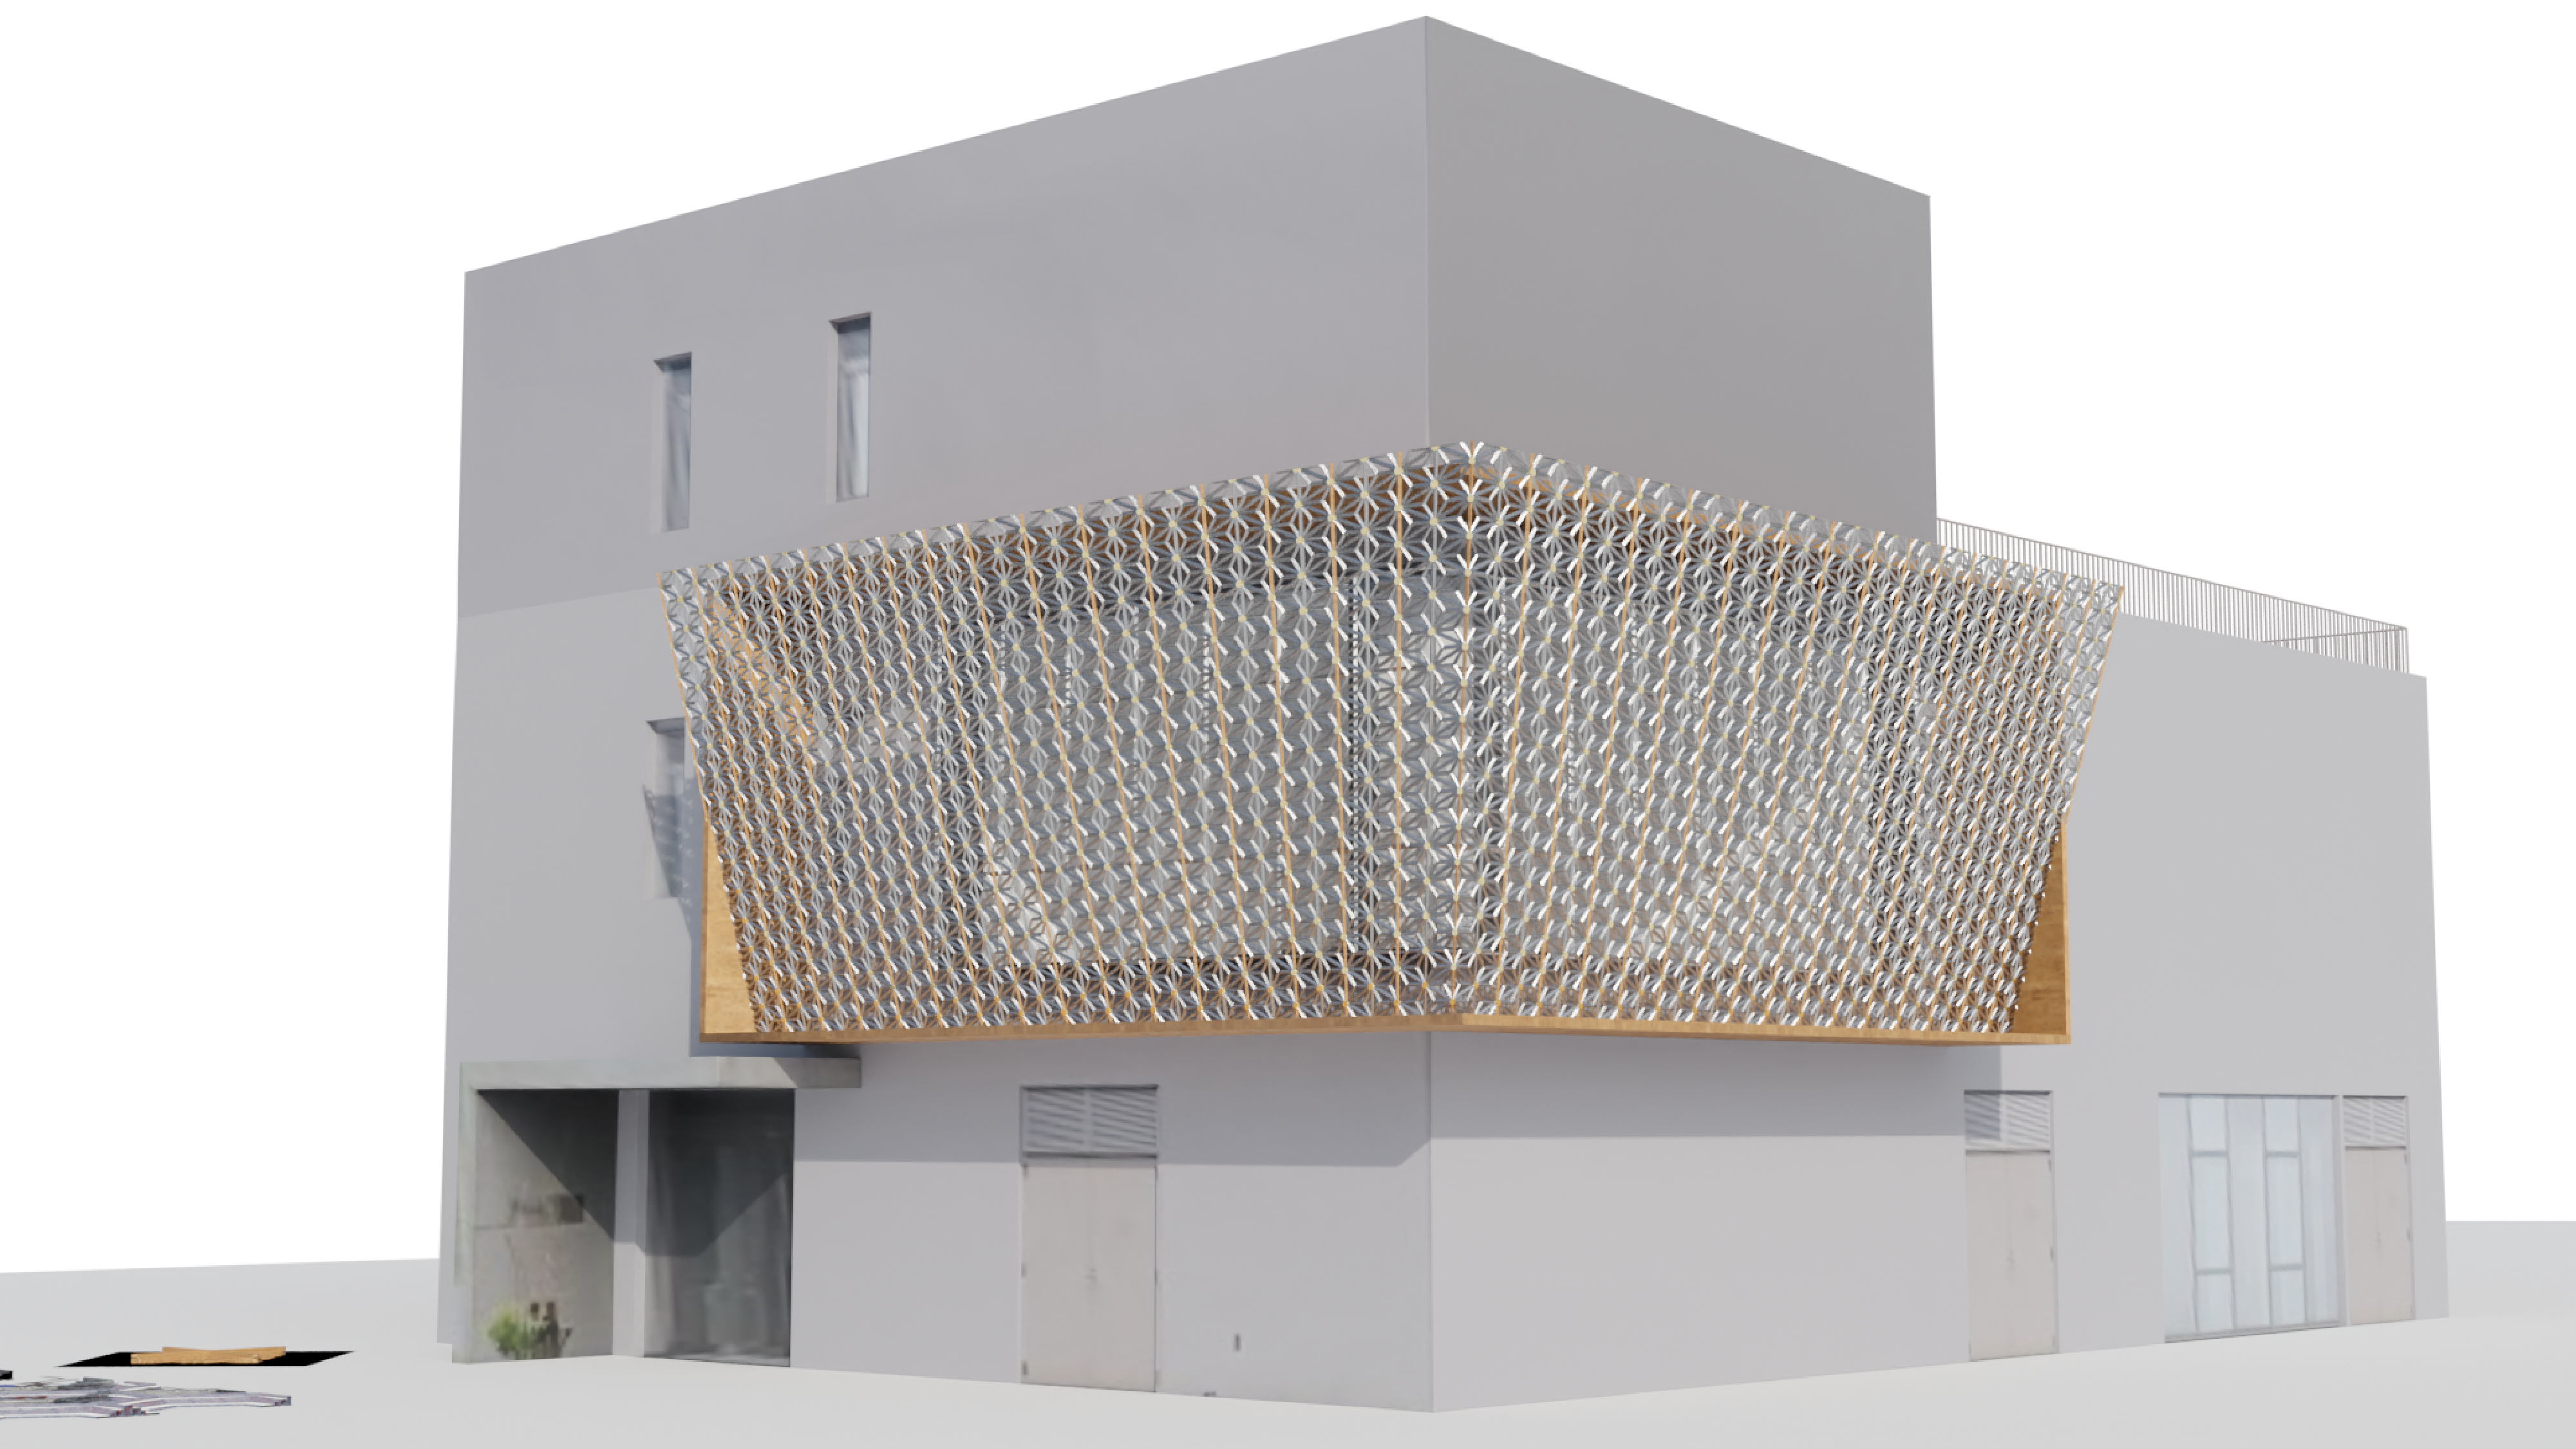
\includegraphics[width=1\linewidth]{Images/Pattern 3/0004}} \\
            \midrule
            \textit{Level 5} &  &  &
            \\
            {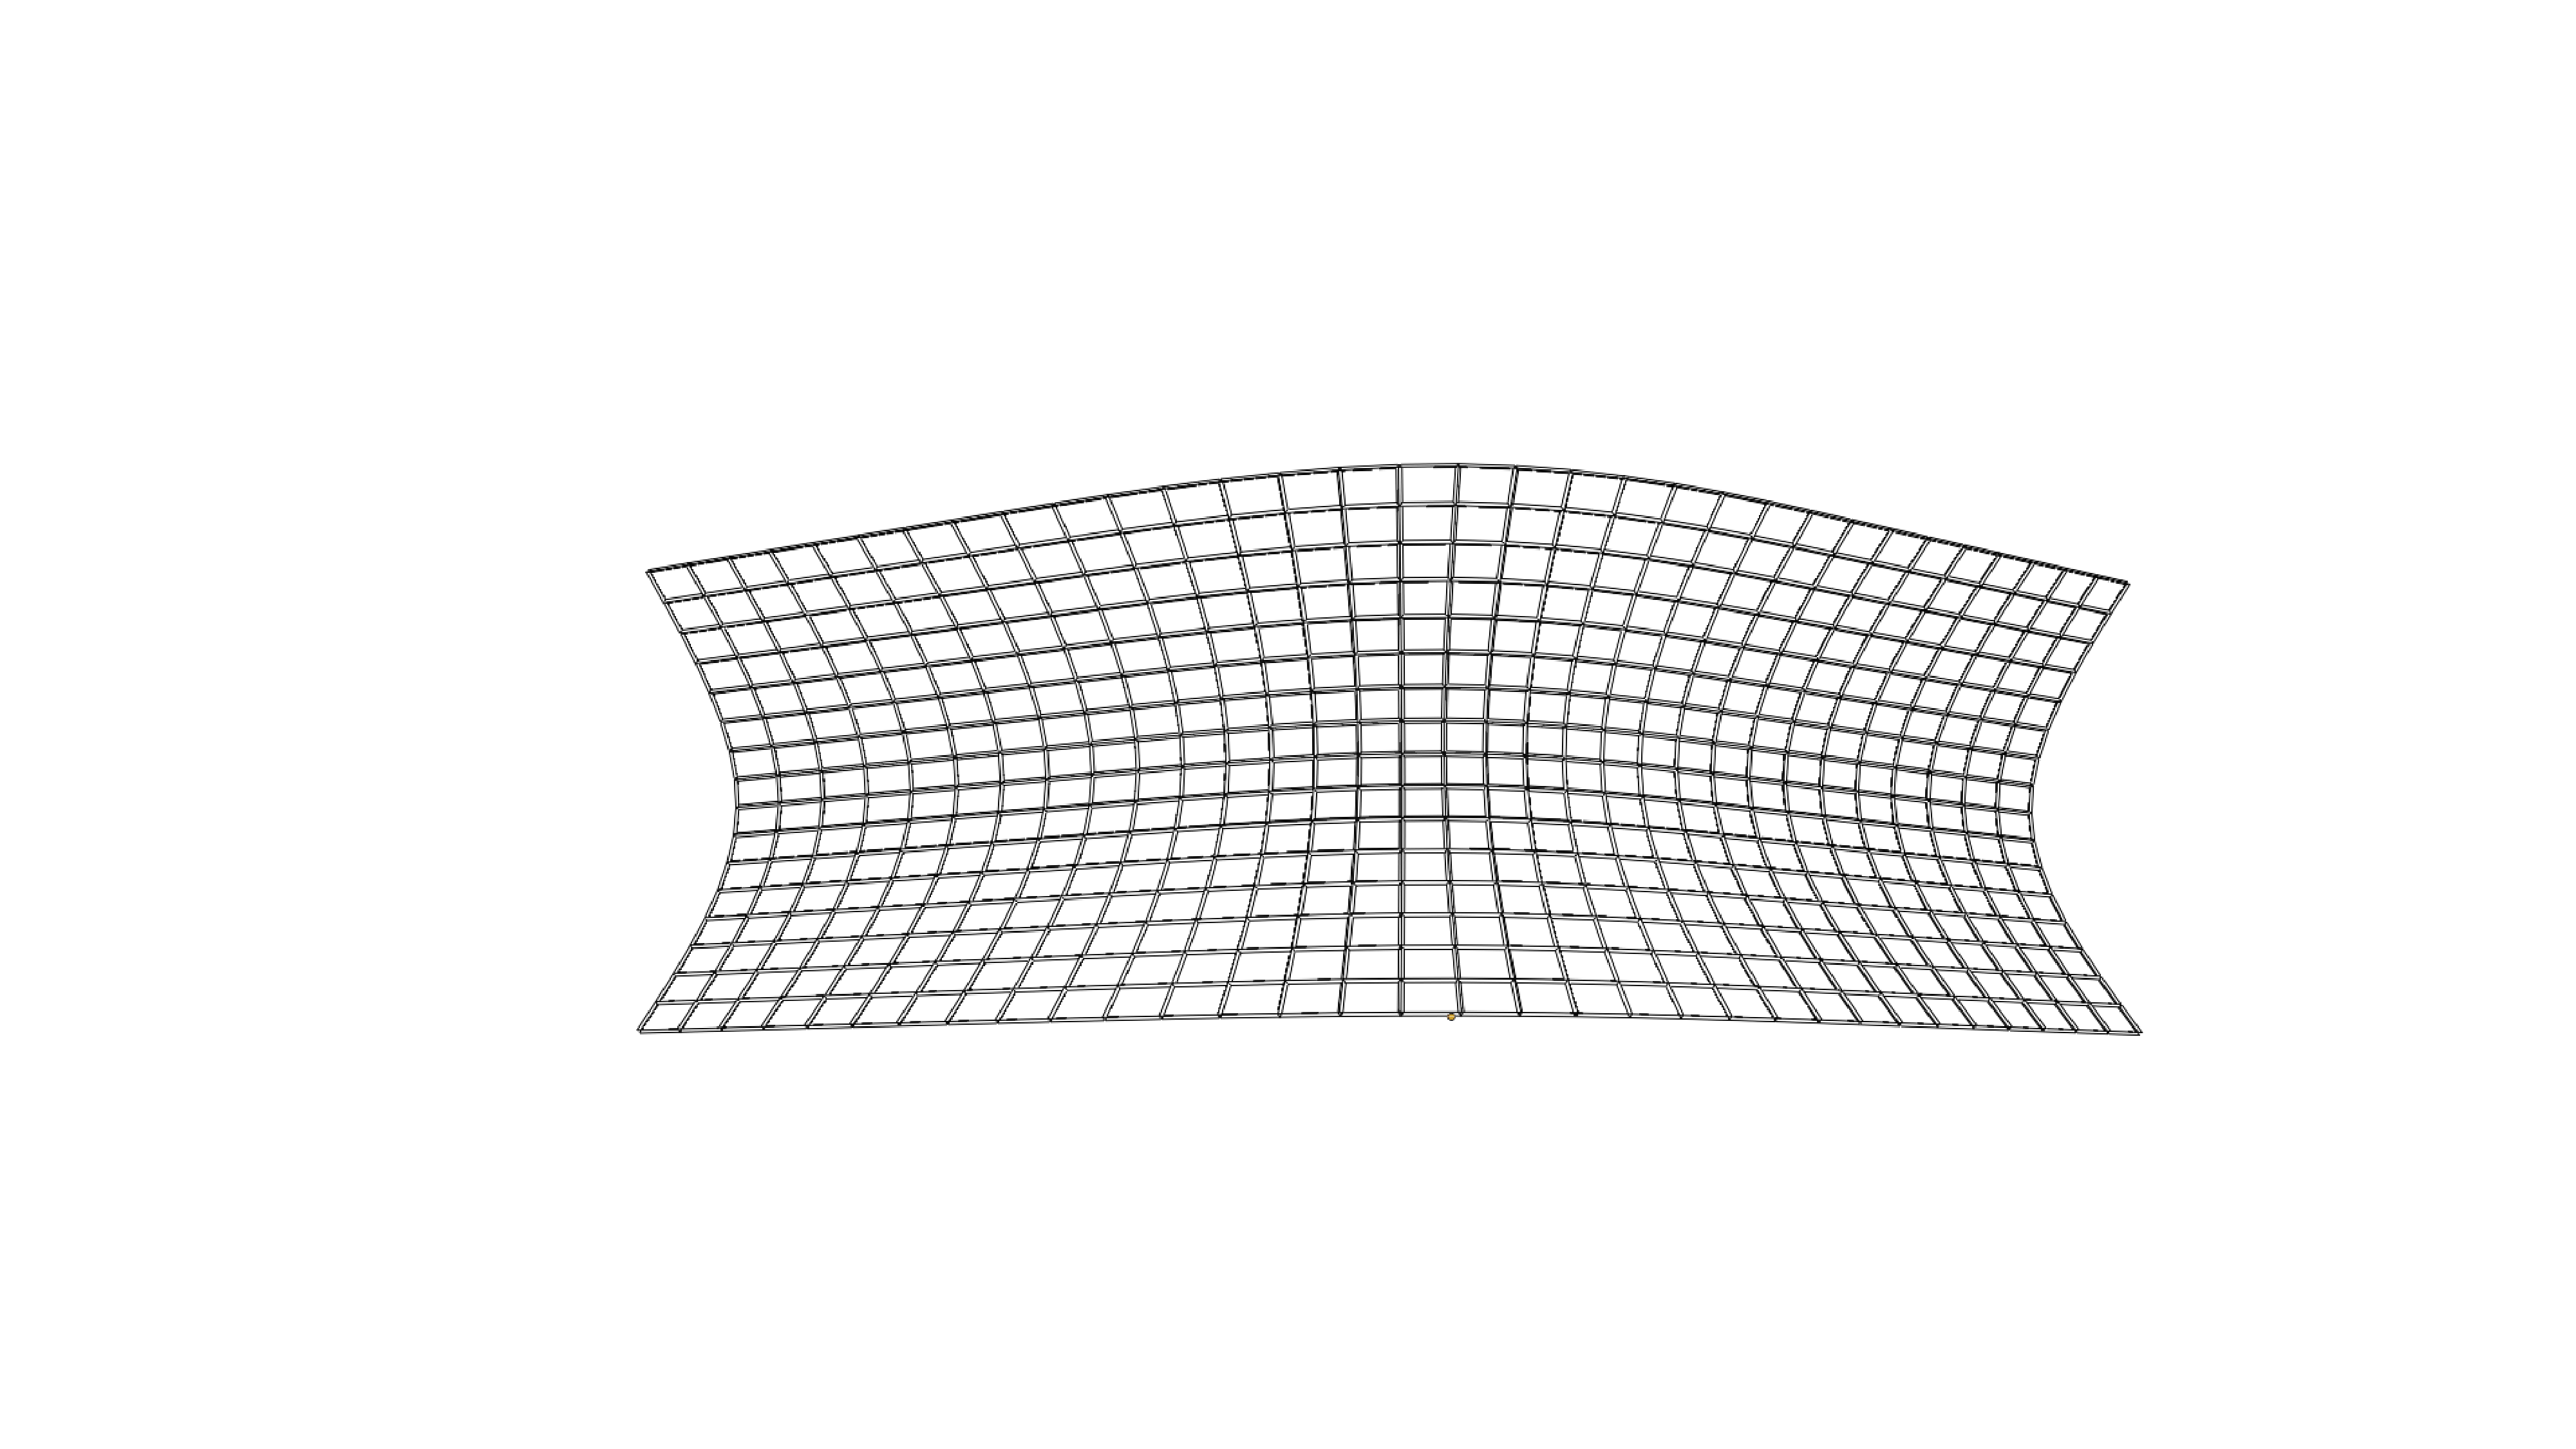
\includegraphics[width=1\linewidth]{Images/Wall 0/0005}} &
              {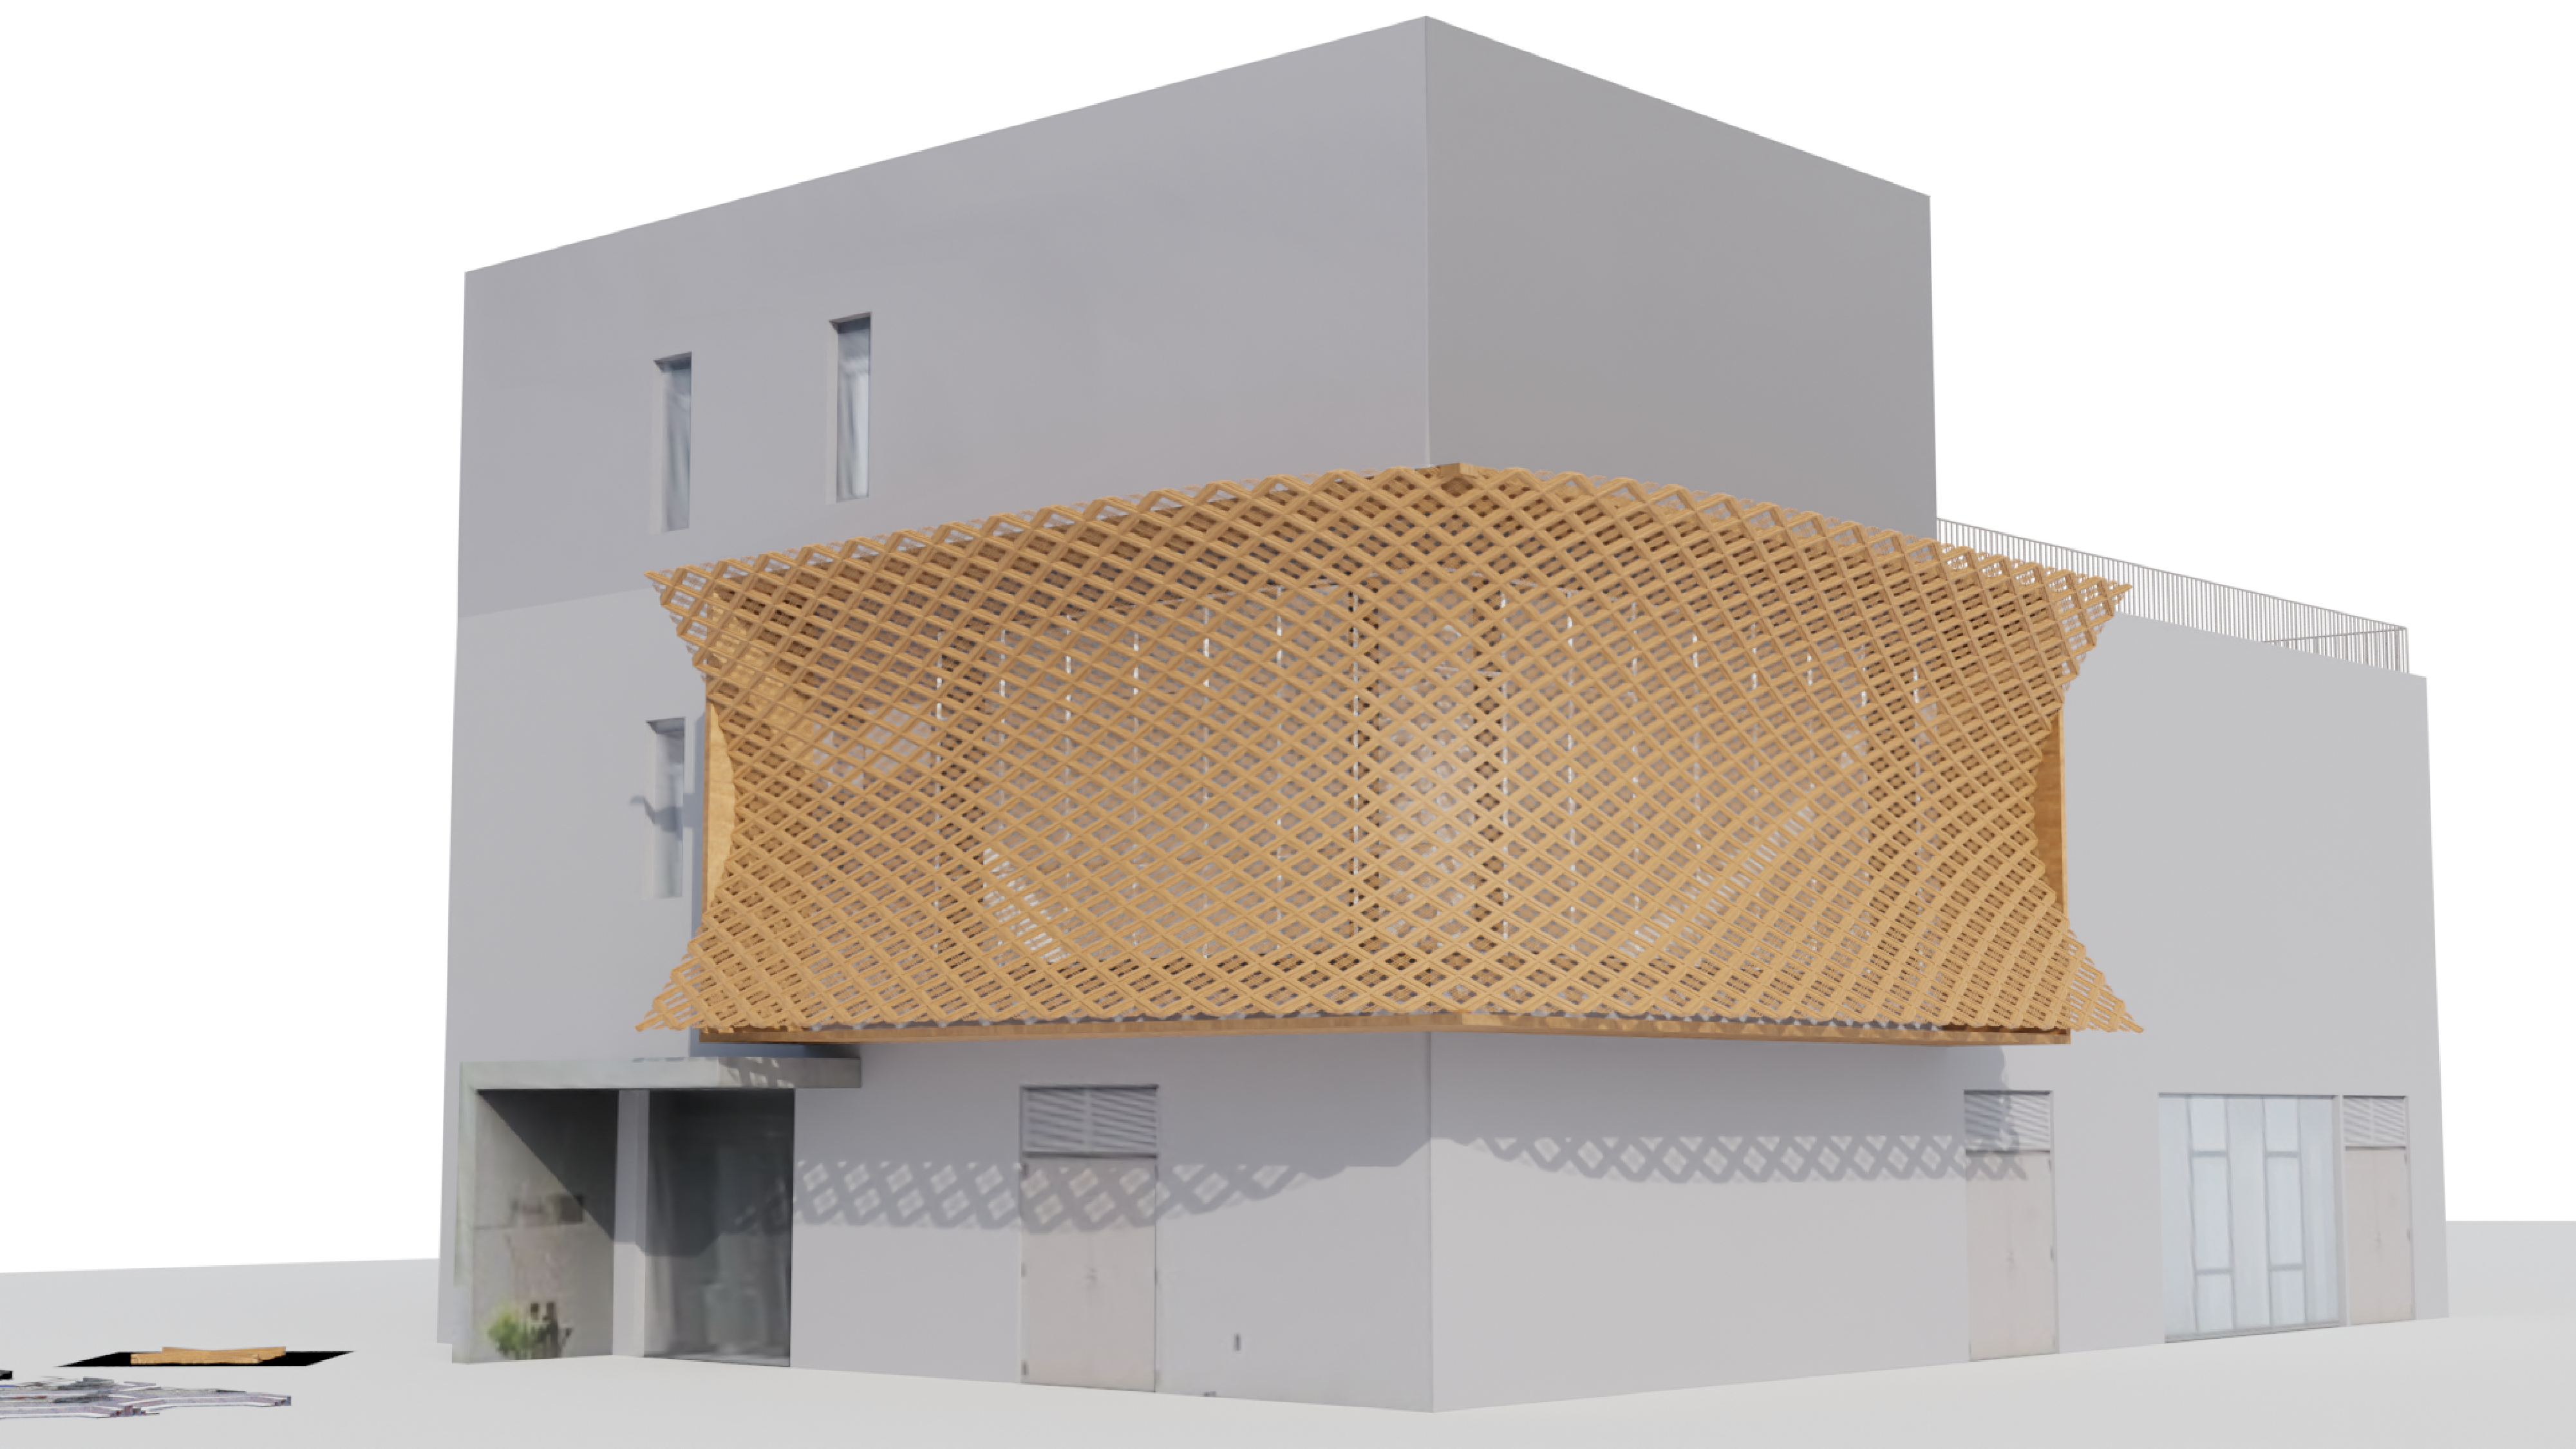
\includegraphics[width=1\linewidth]{Images/Pattern 1/0005}} &
              {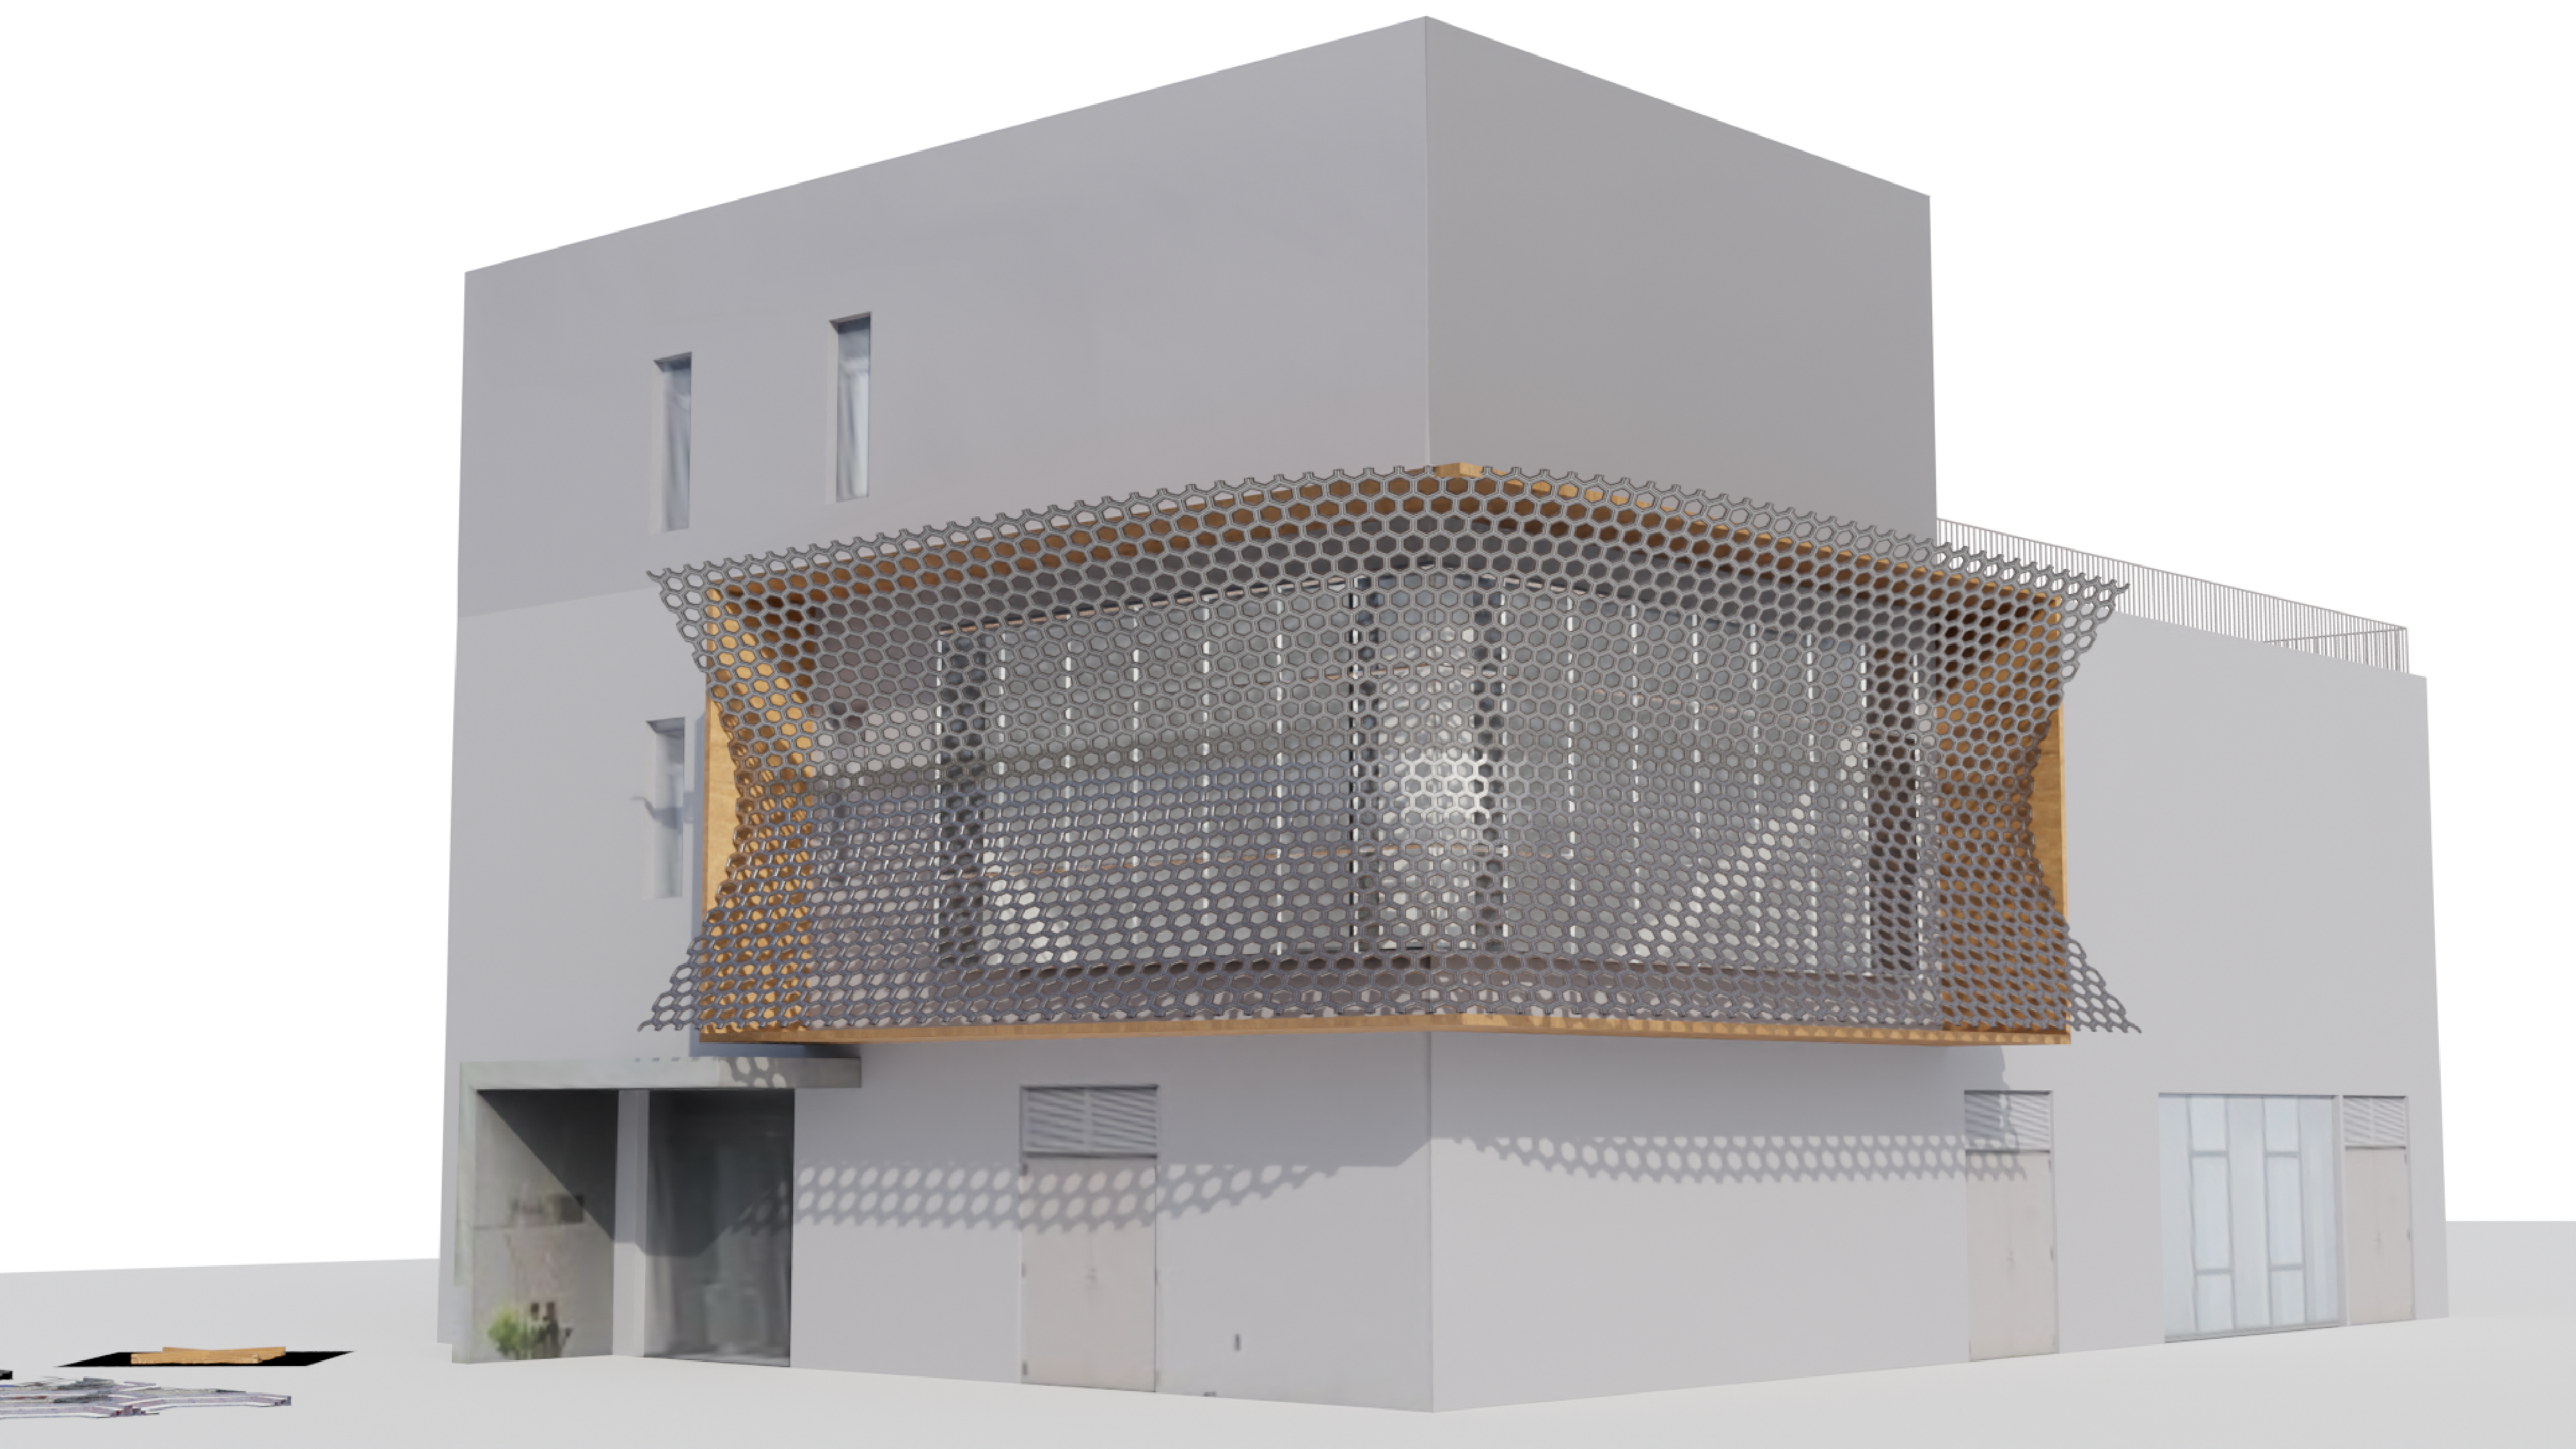
\includegraphics[width=1\linewidth]{Images/Pattern 2/0005}} &
              {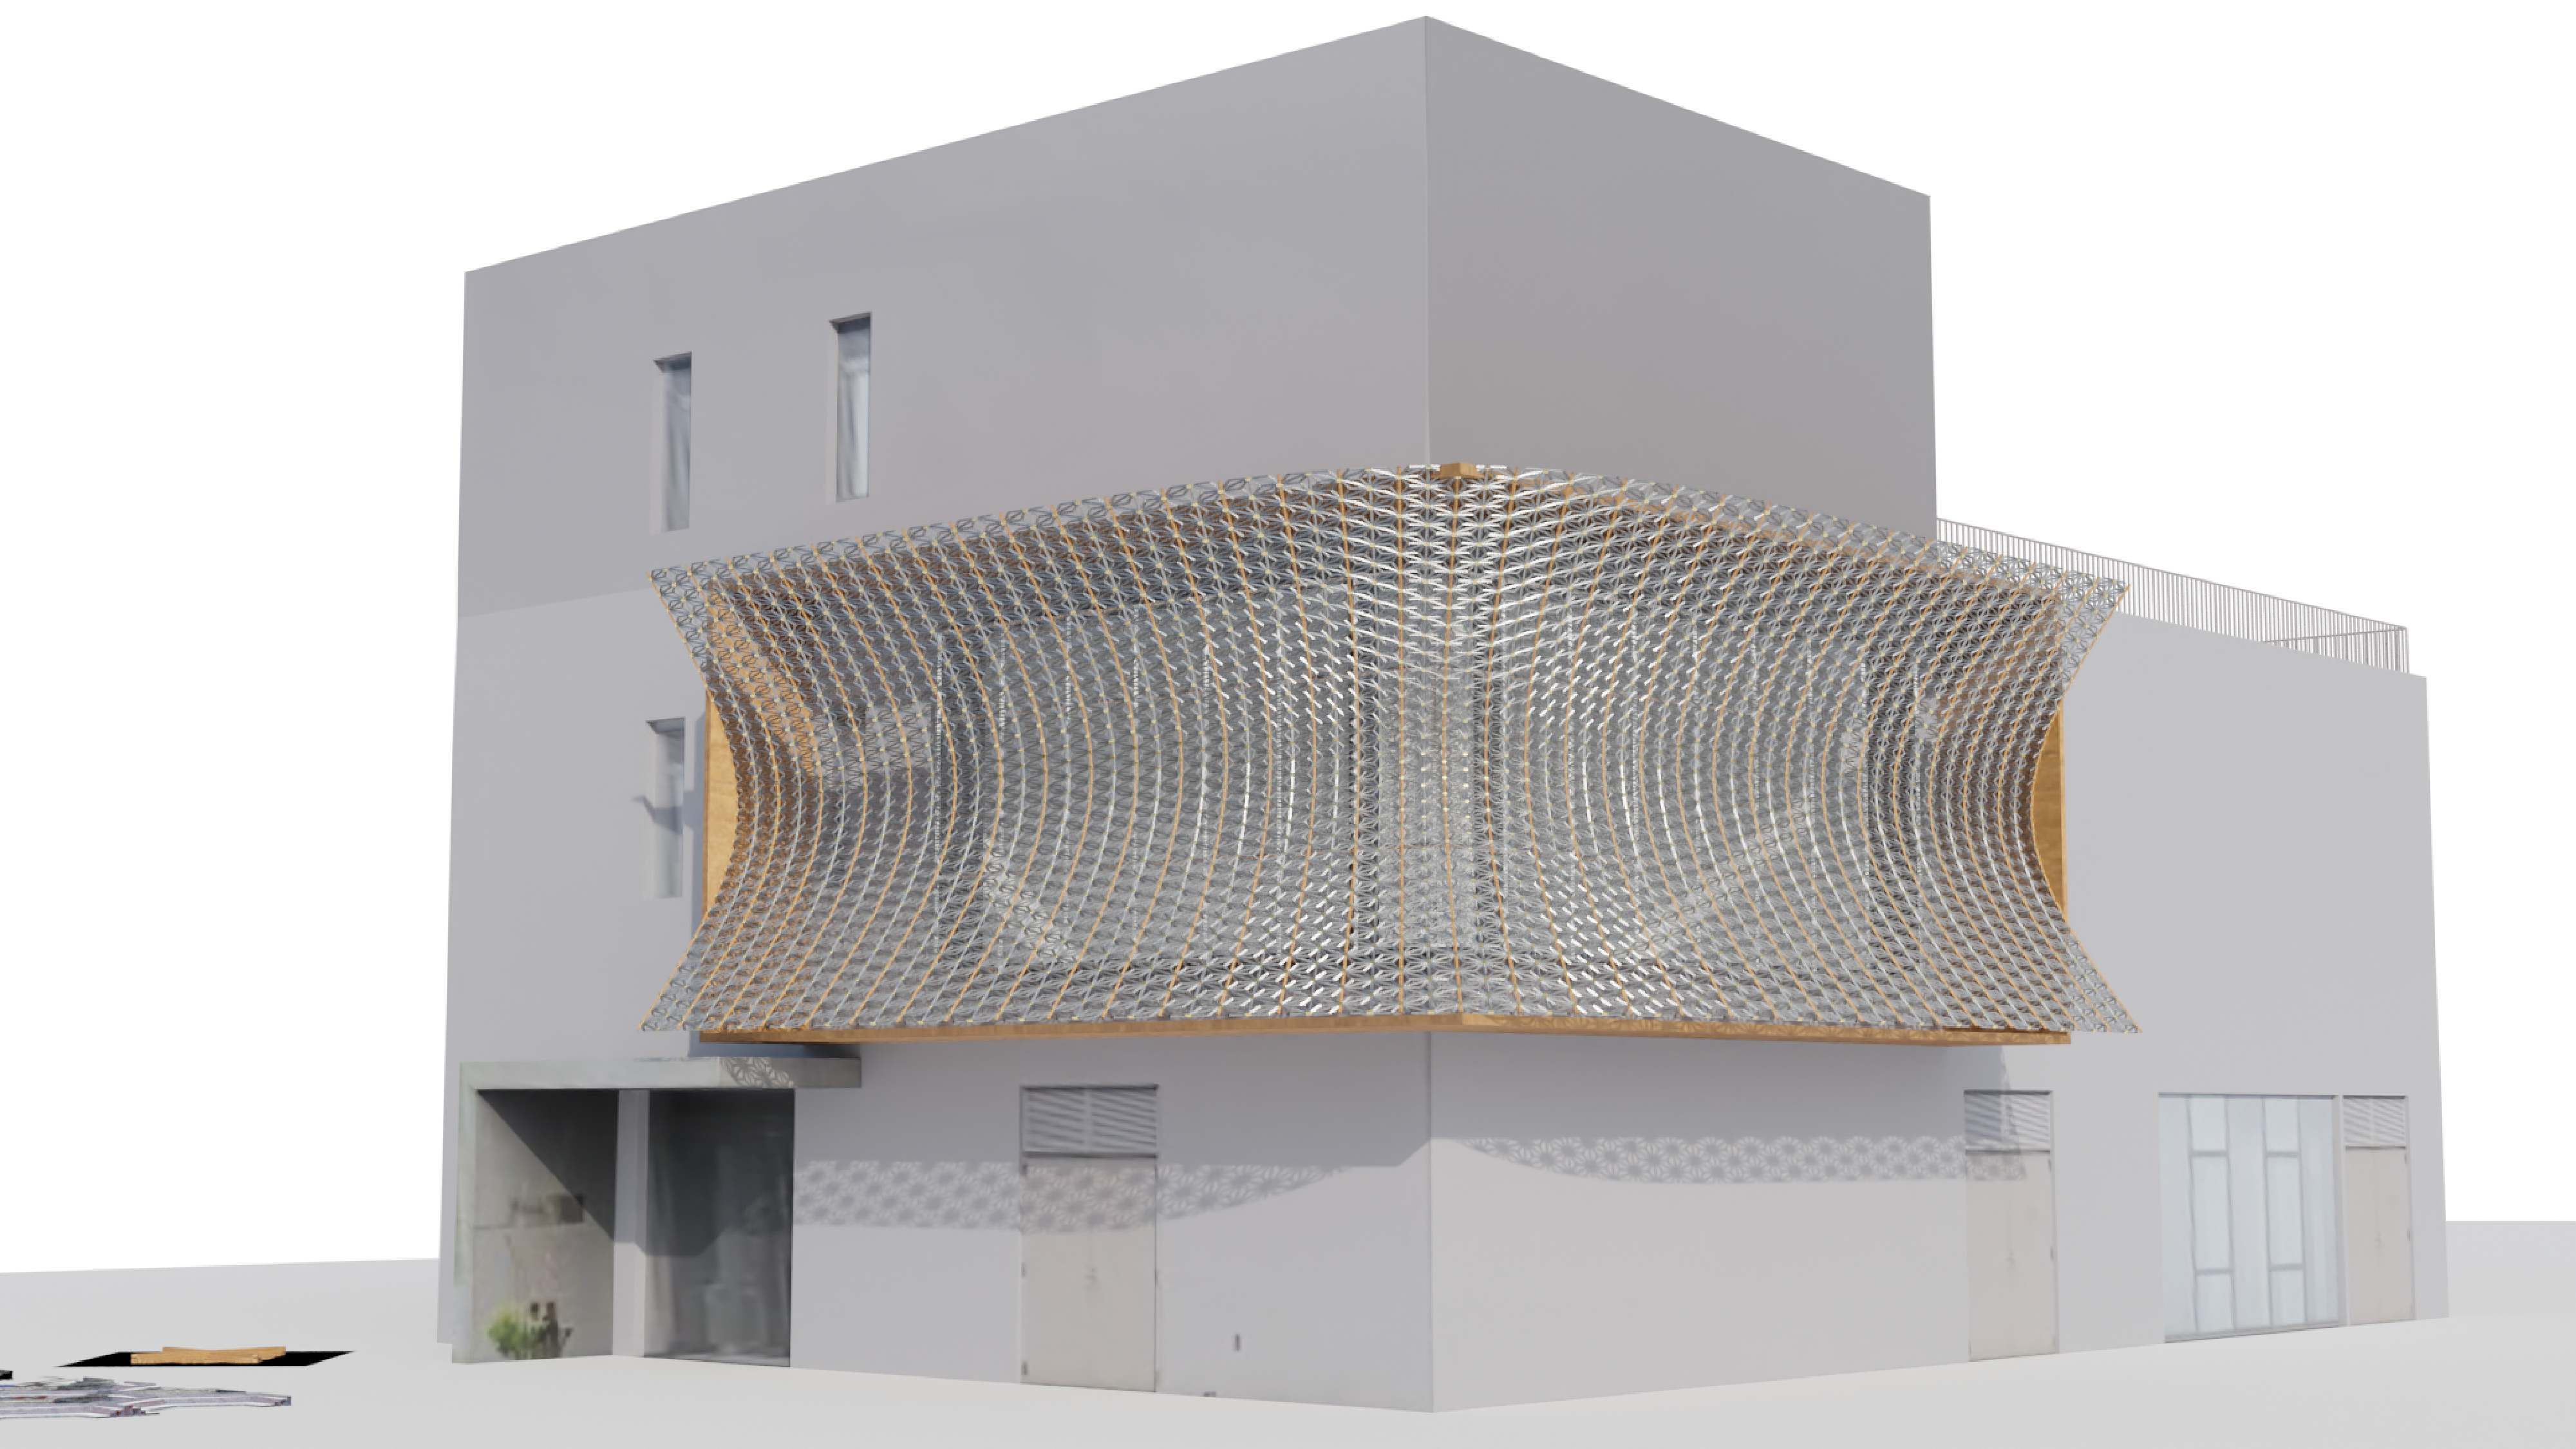
\includegraphics[width=1\linewidth]{Images/Pattern 3/0005}} \\
            \bottomrule
        \end{tabularx}
    \end{table*}

    %%Table: Pattern Variations 6 to 10. Part2
    \begin{table*}[htb]
        \centering
        \small
        \caption{Patterns variations for the last five levels of complexity}
        \label{tab:PatternsVariationsPart2}
        \begin{tabularx}
        {\textwidth}{p{3cm} >{\centering\arraybackslash}X >{\centering\arraybackslash}X >{\centering\arraybackslash}X }
            \toprule
            \textit{Description} &
              \textit{Pattern 1} &
              \textit{Pattern 2} &
              \textit{Pattern 3} \\
            \midrule
            \text{Pattern Name} & Hishi Pattern & Tortoise shells & Asanoha Pattern\\

            \midrule
            \textit{Base Module} &  &  &
            \\
            {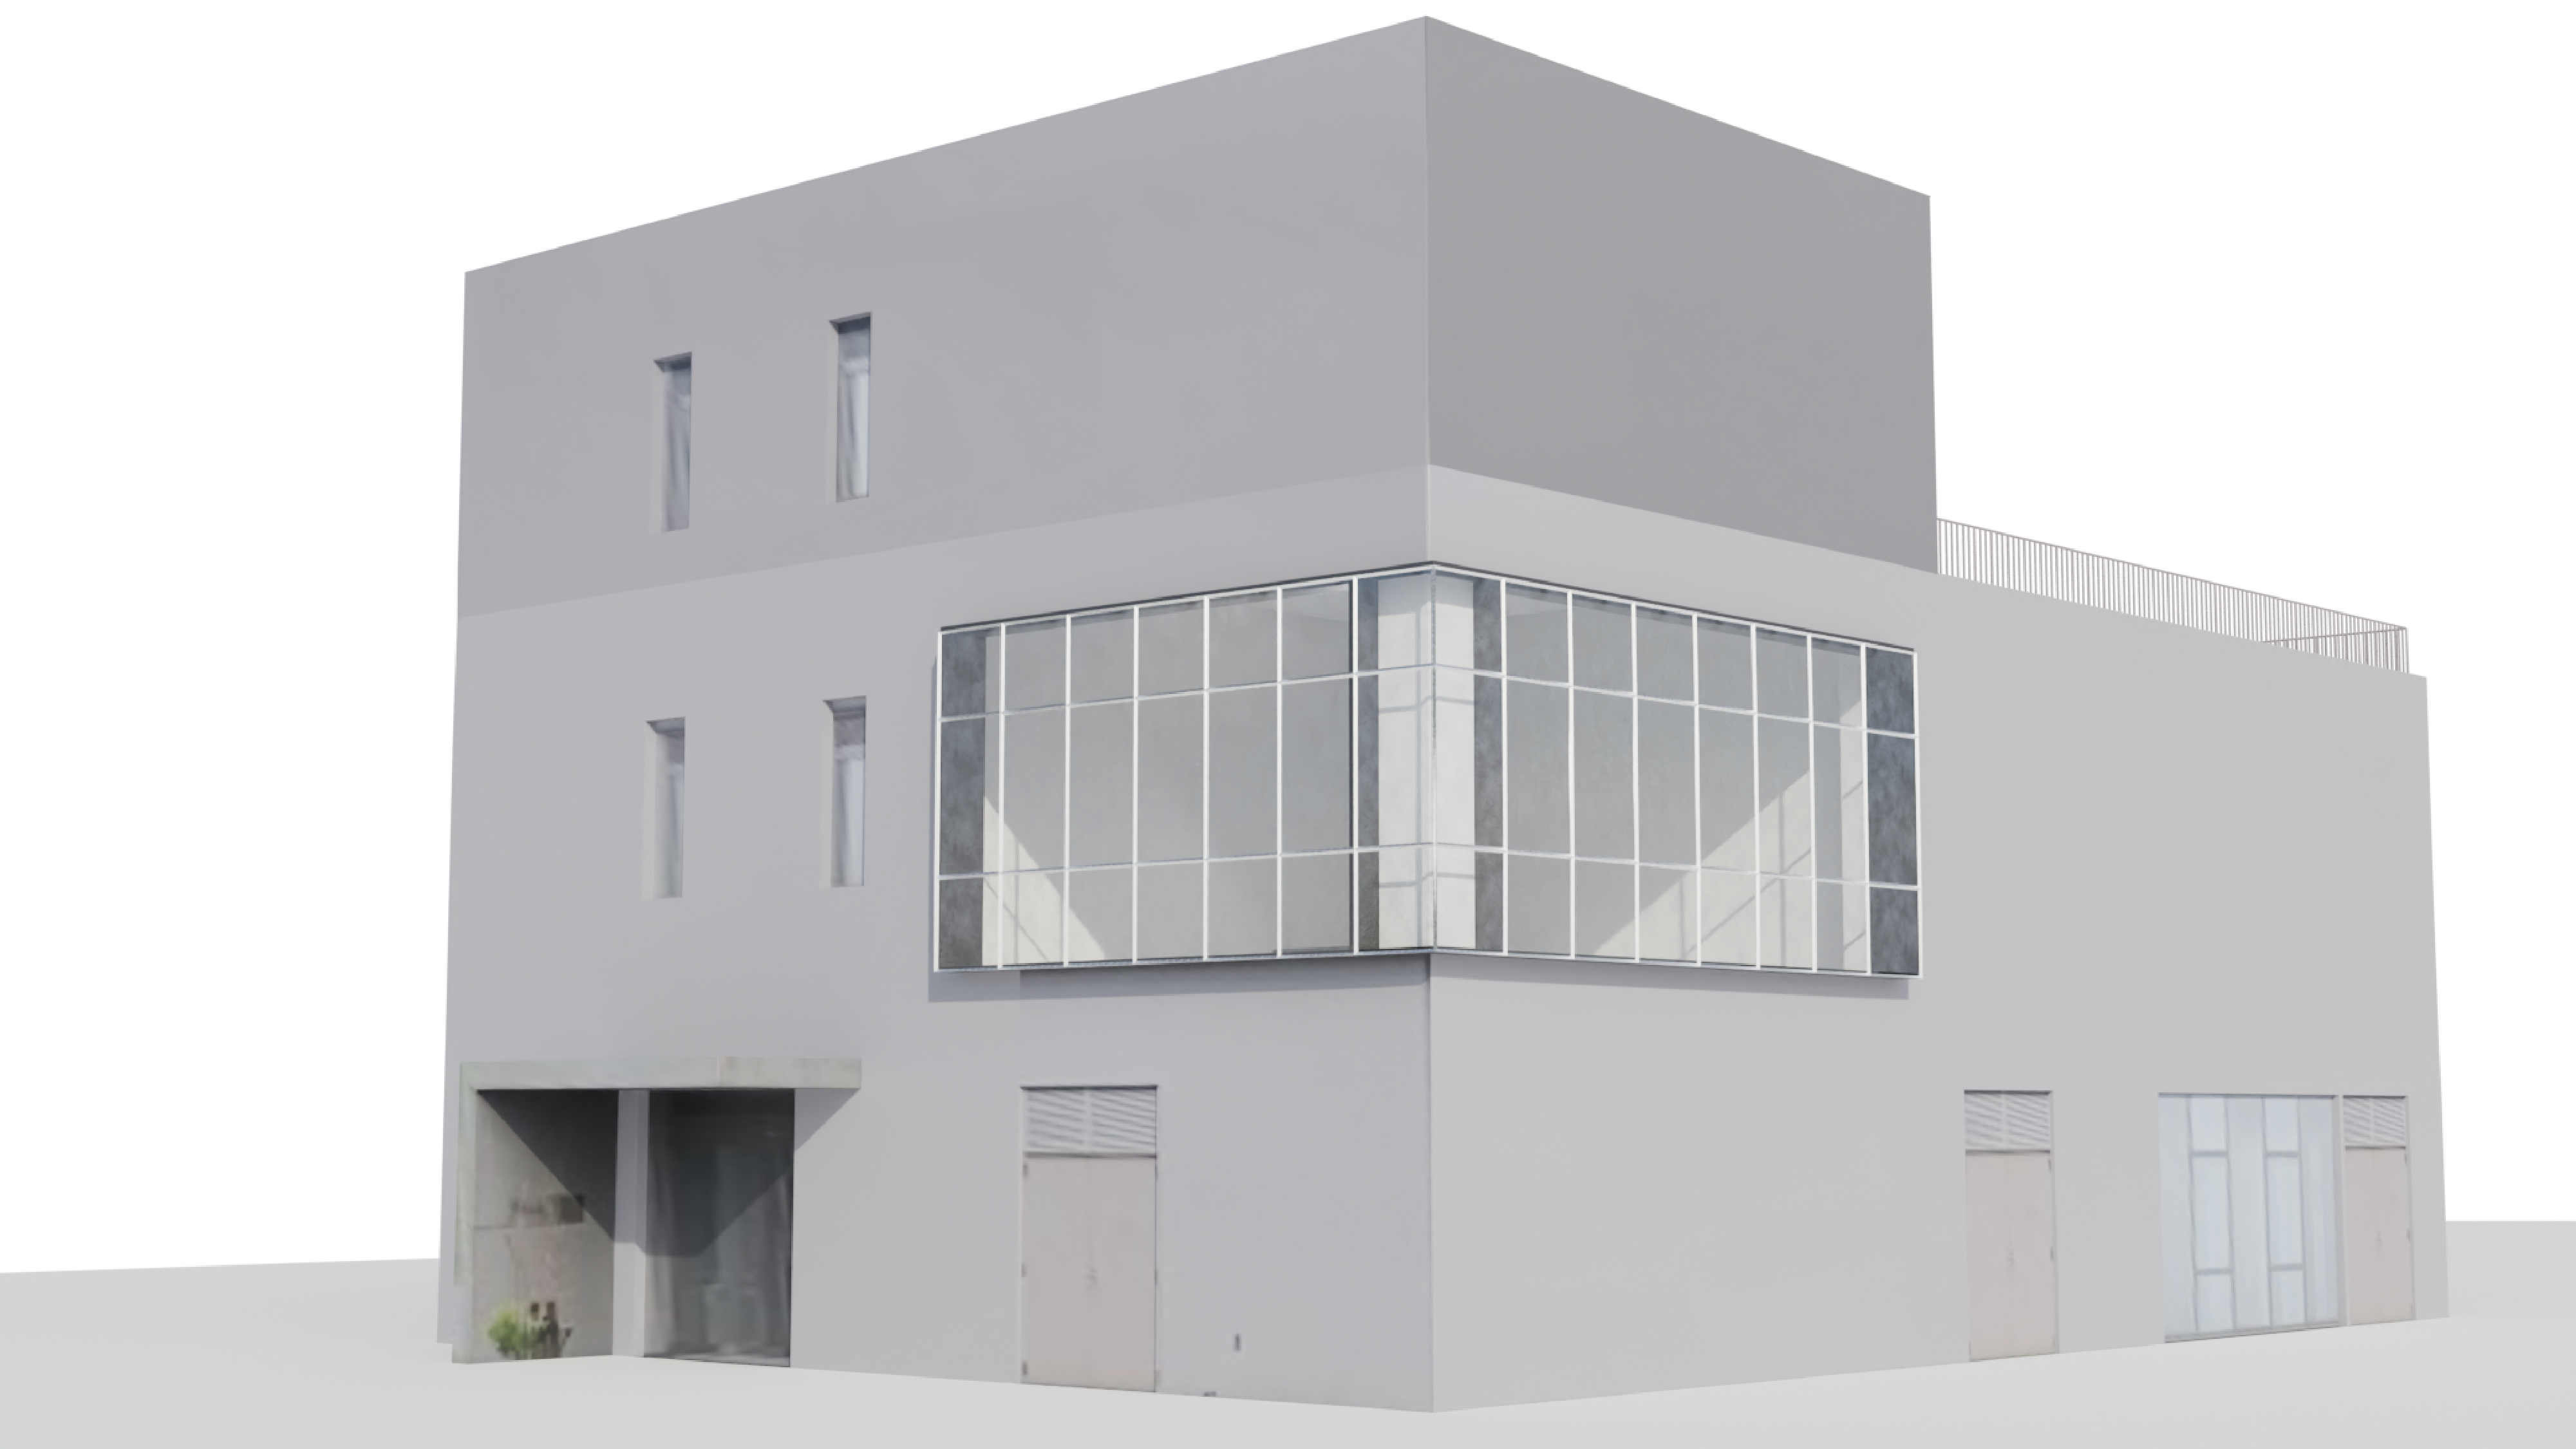
\includegraphics[width=1\linewidth]{Images/Base Module/Building}} &
              {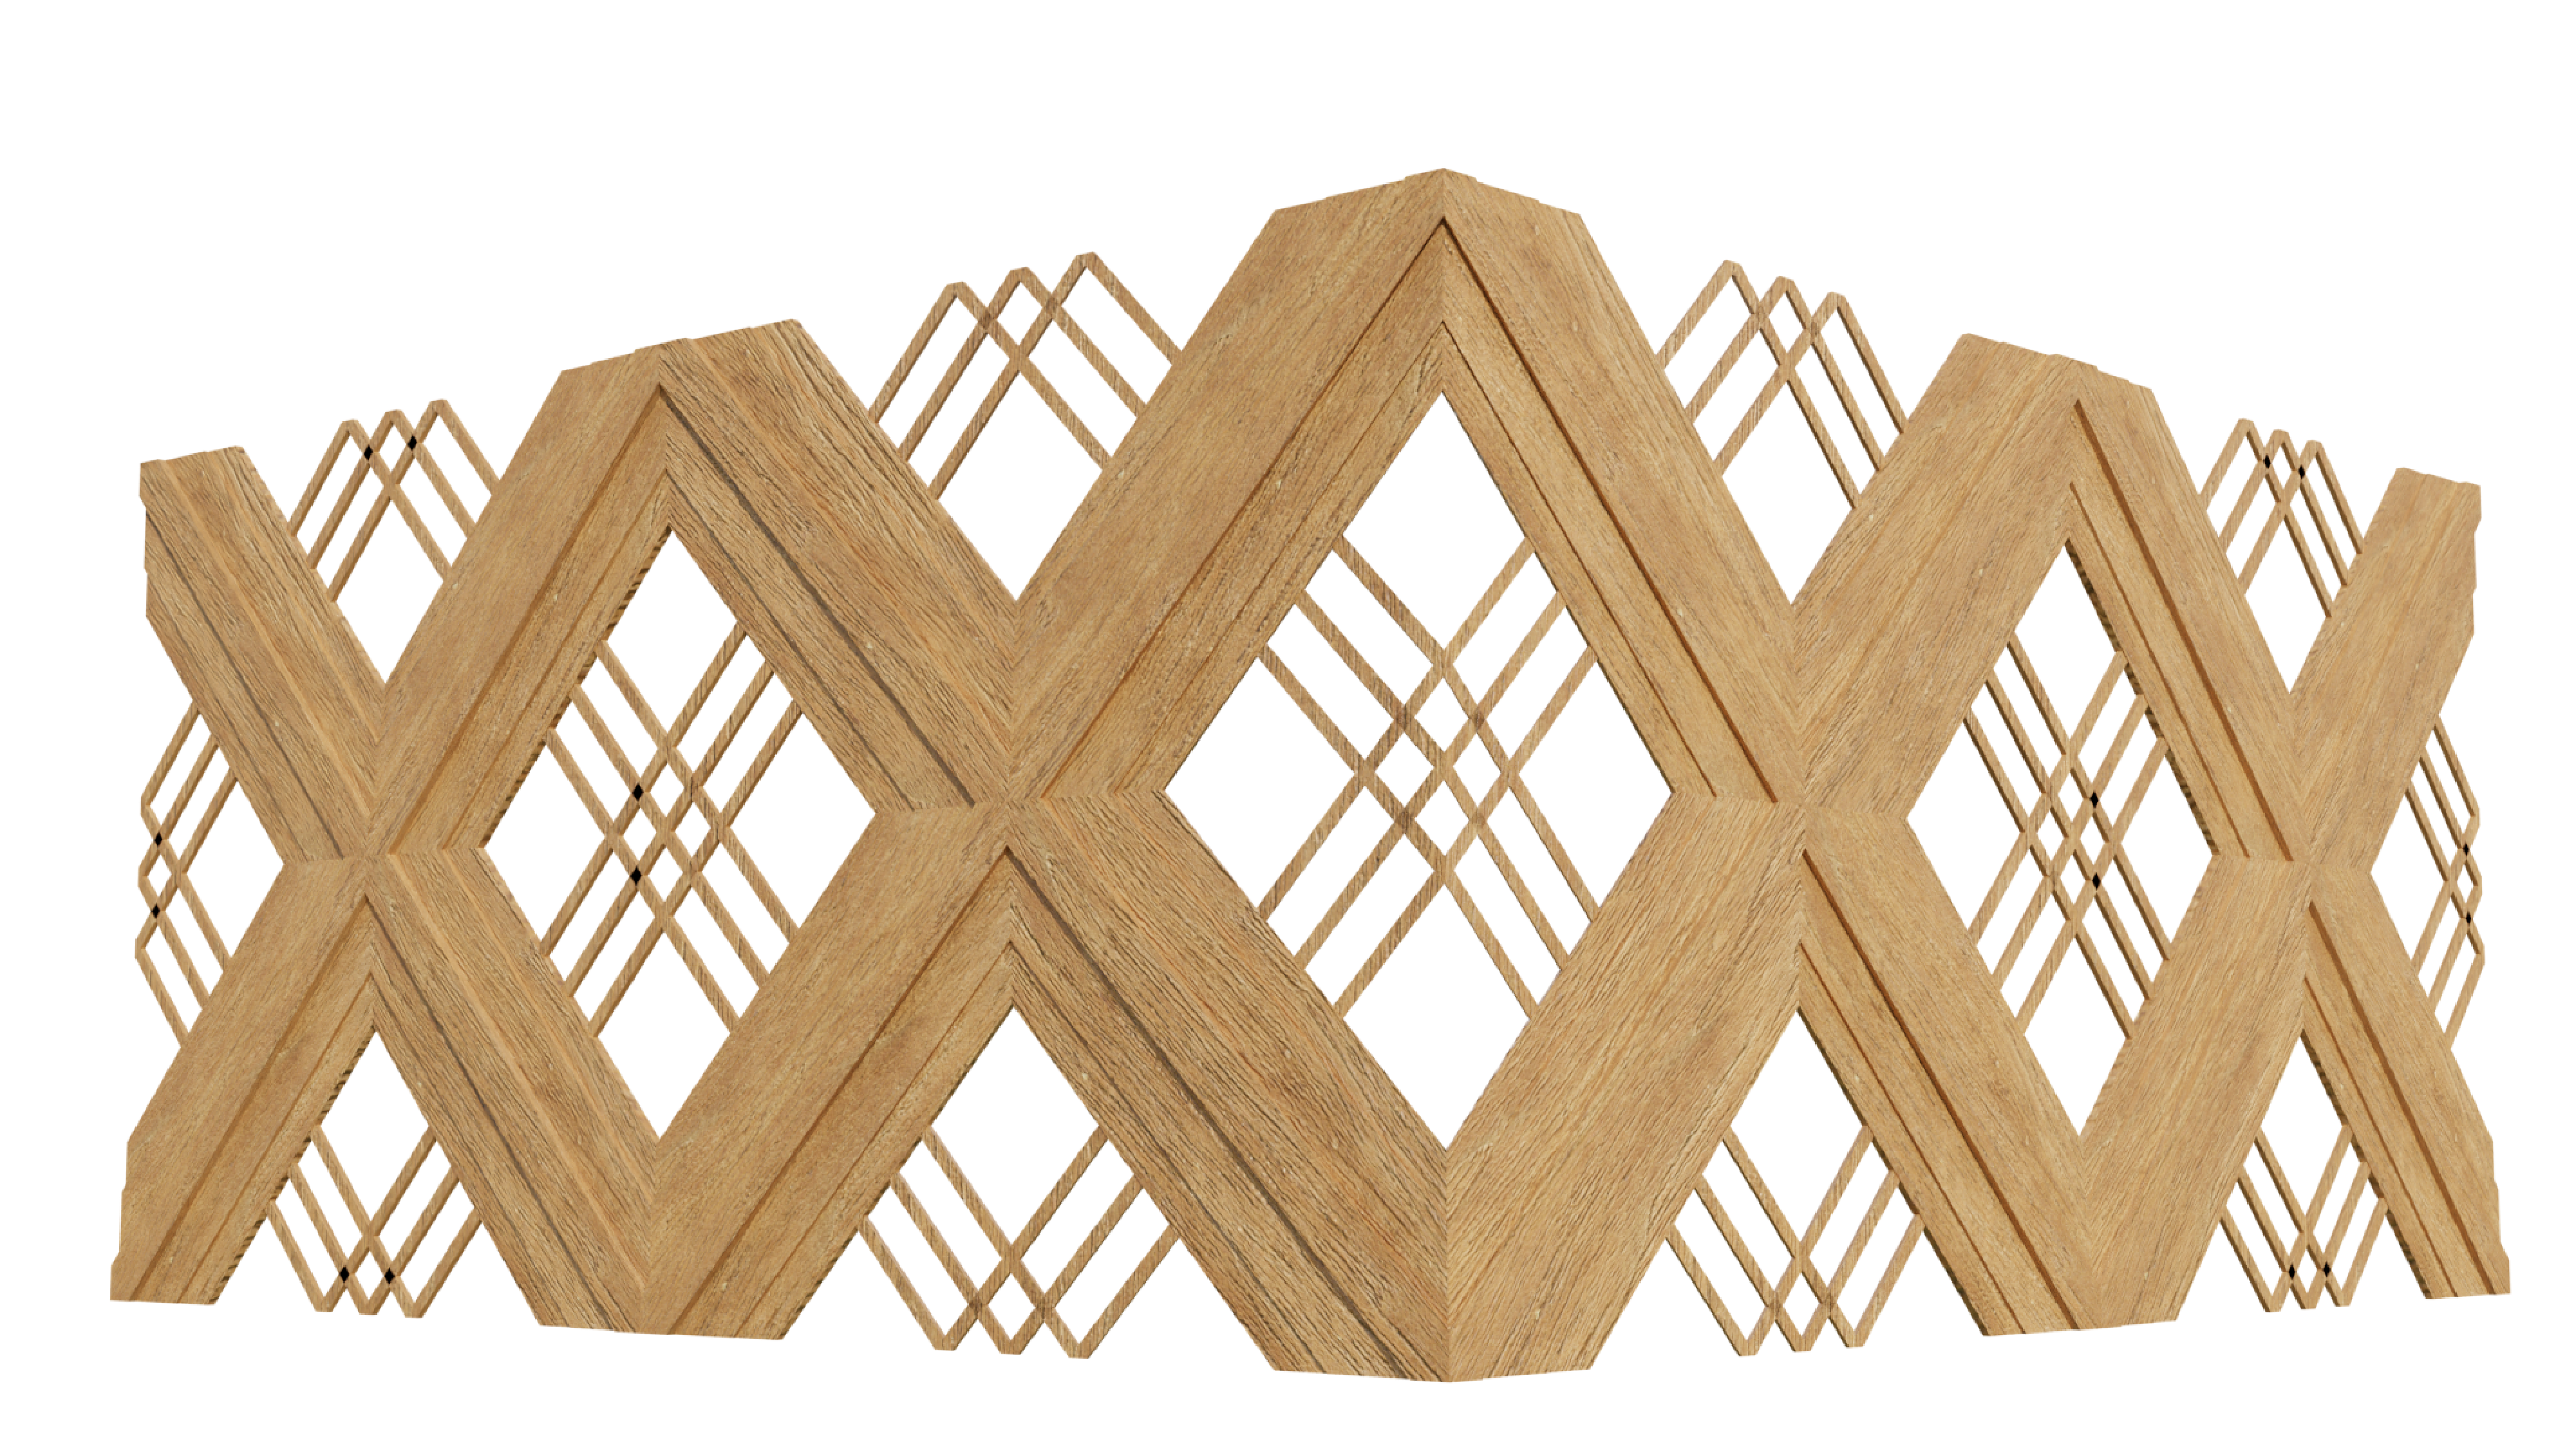
\includegraphics[width=1\linewidth]{Images/Base Module/Pattern1}} &
              {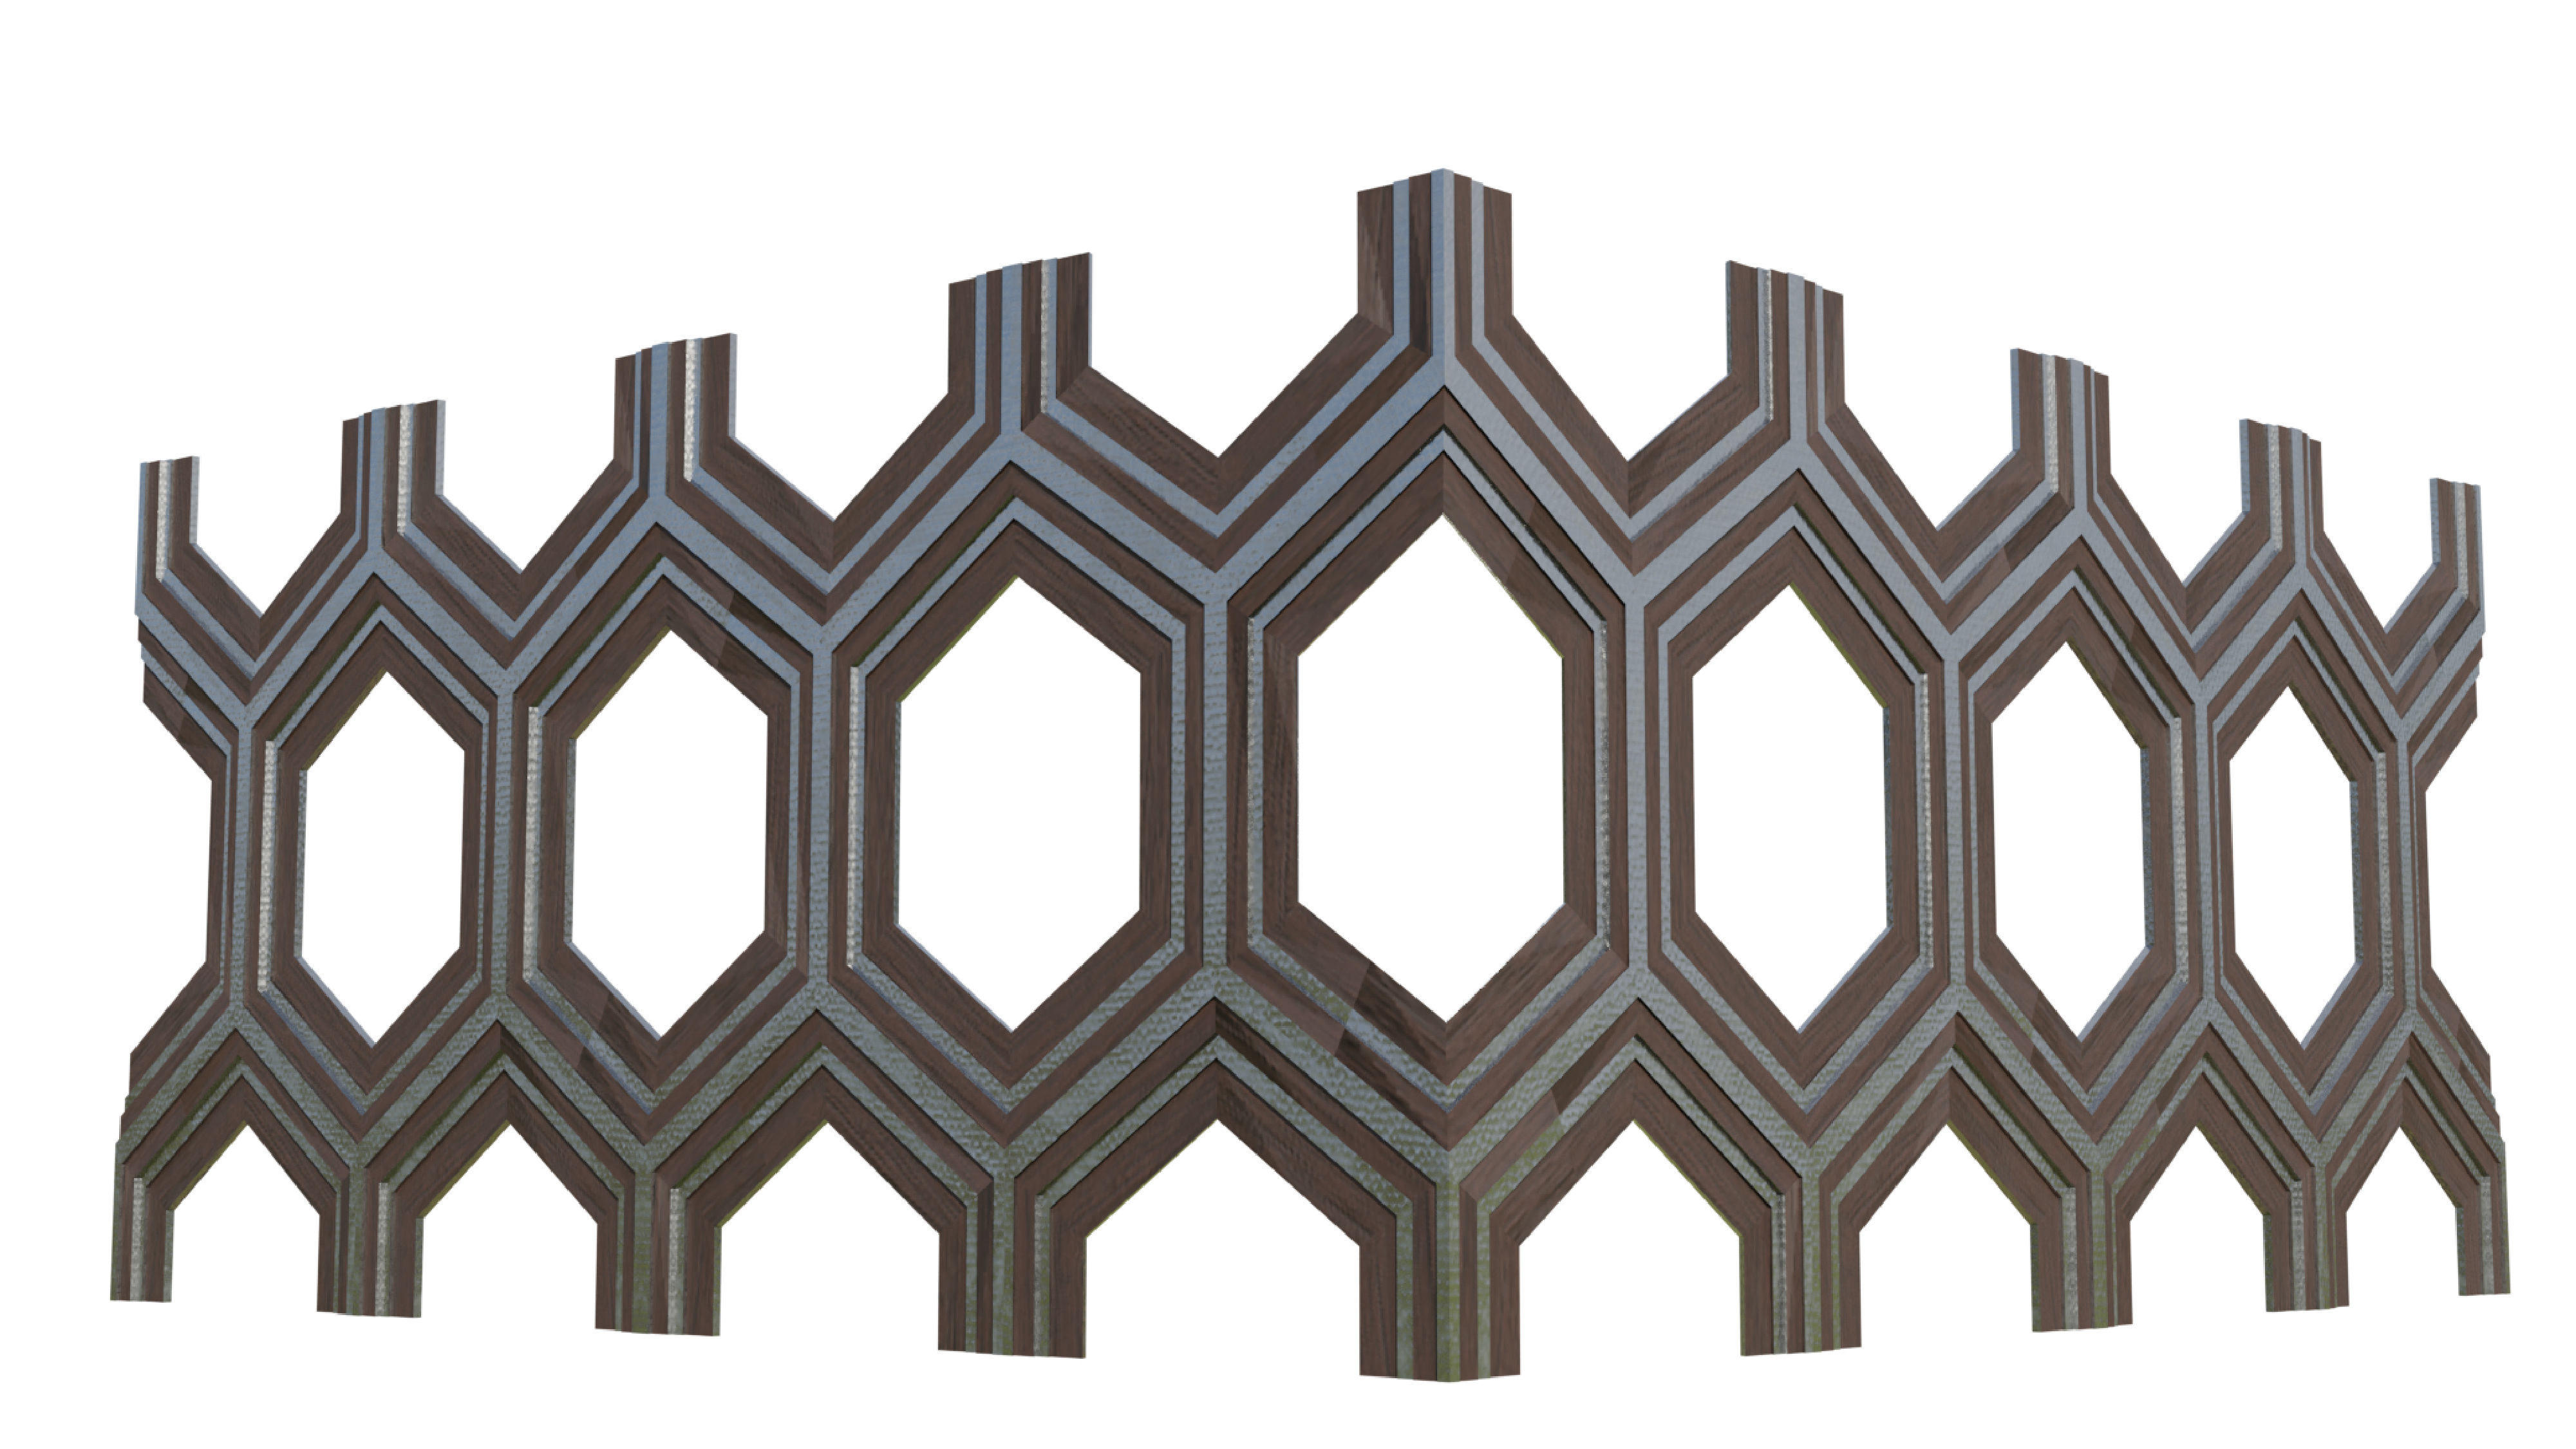
\includegraphics[width=1\linewidth]{Images/Base Module/Pattern2}} &
              {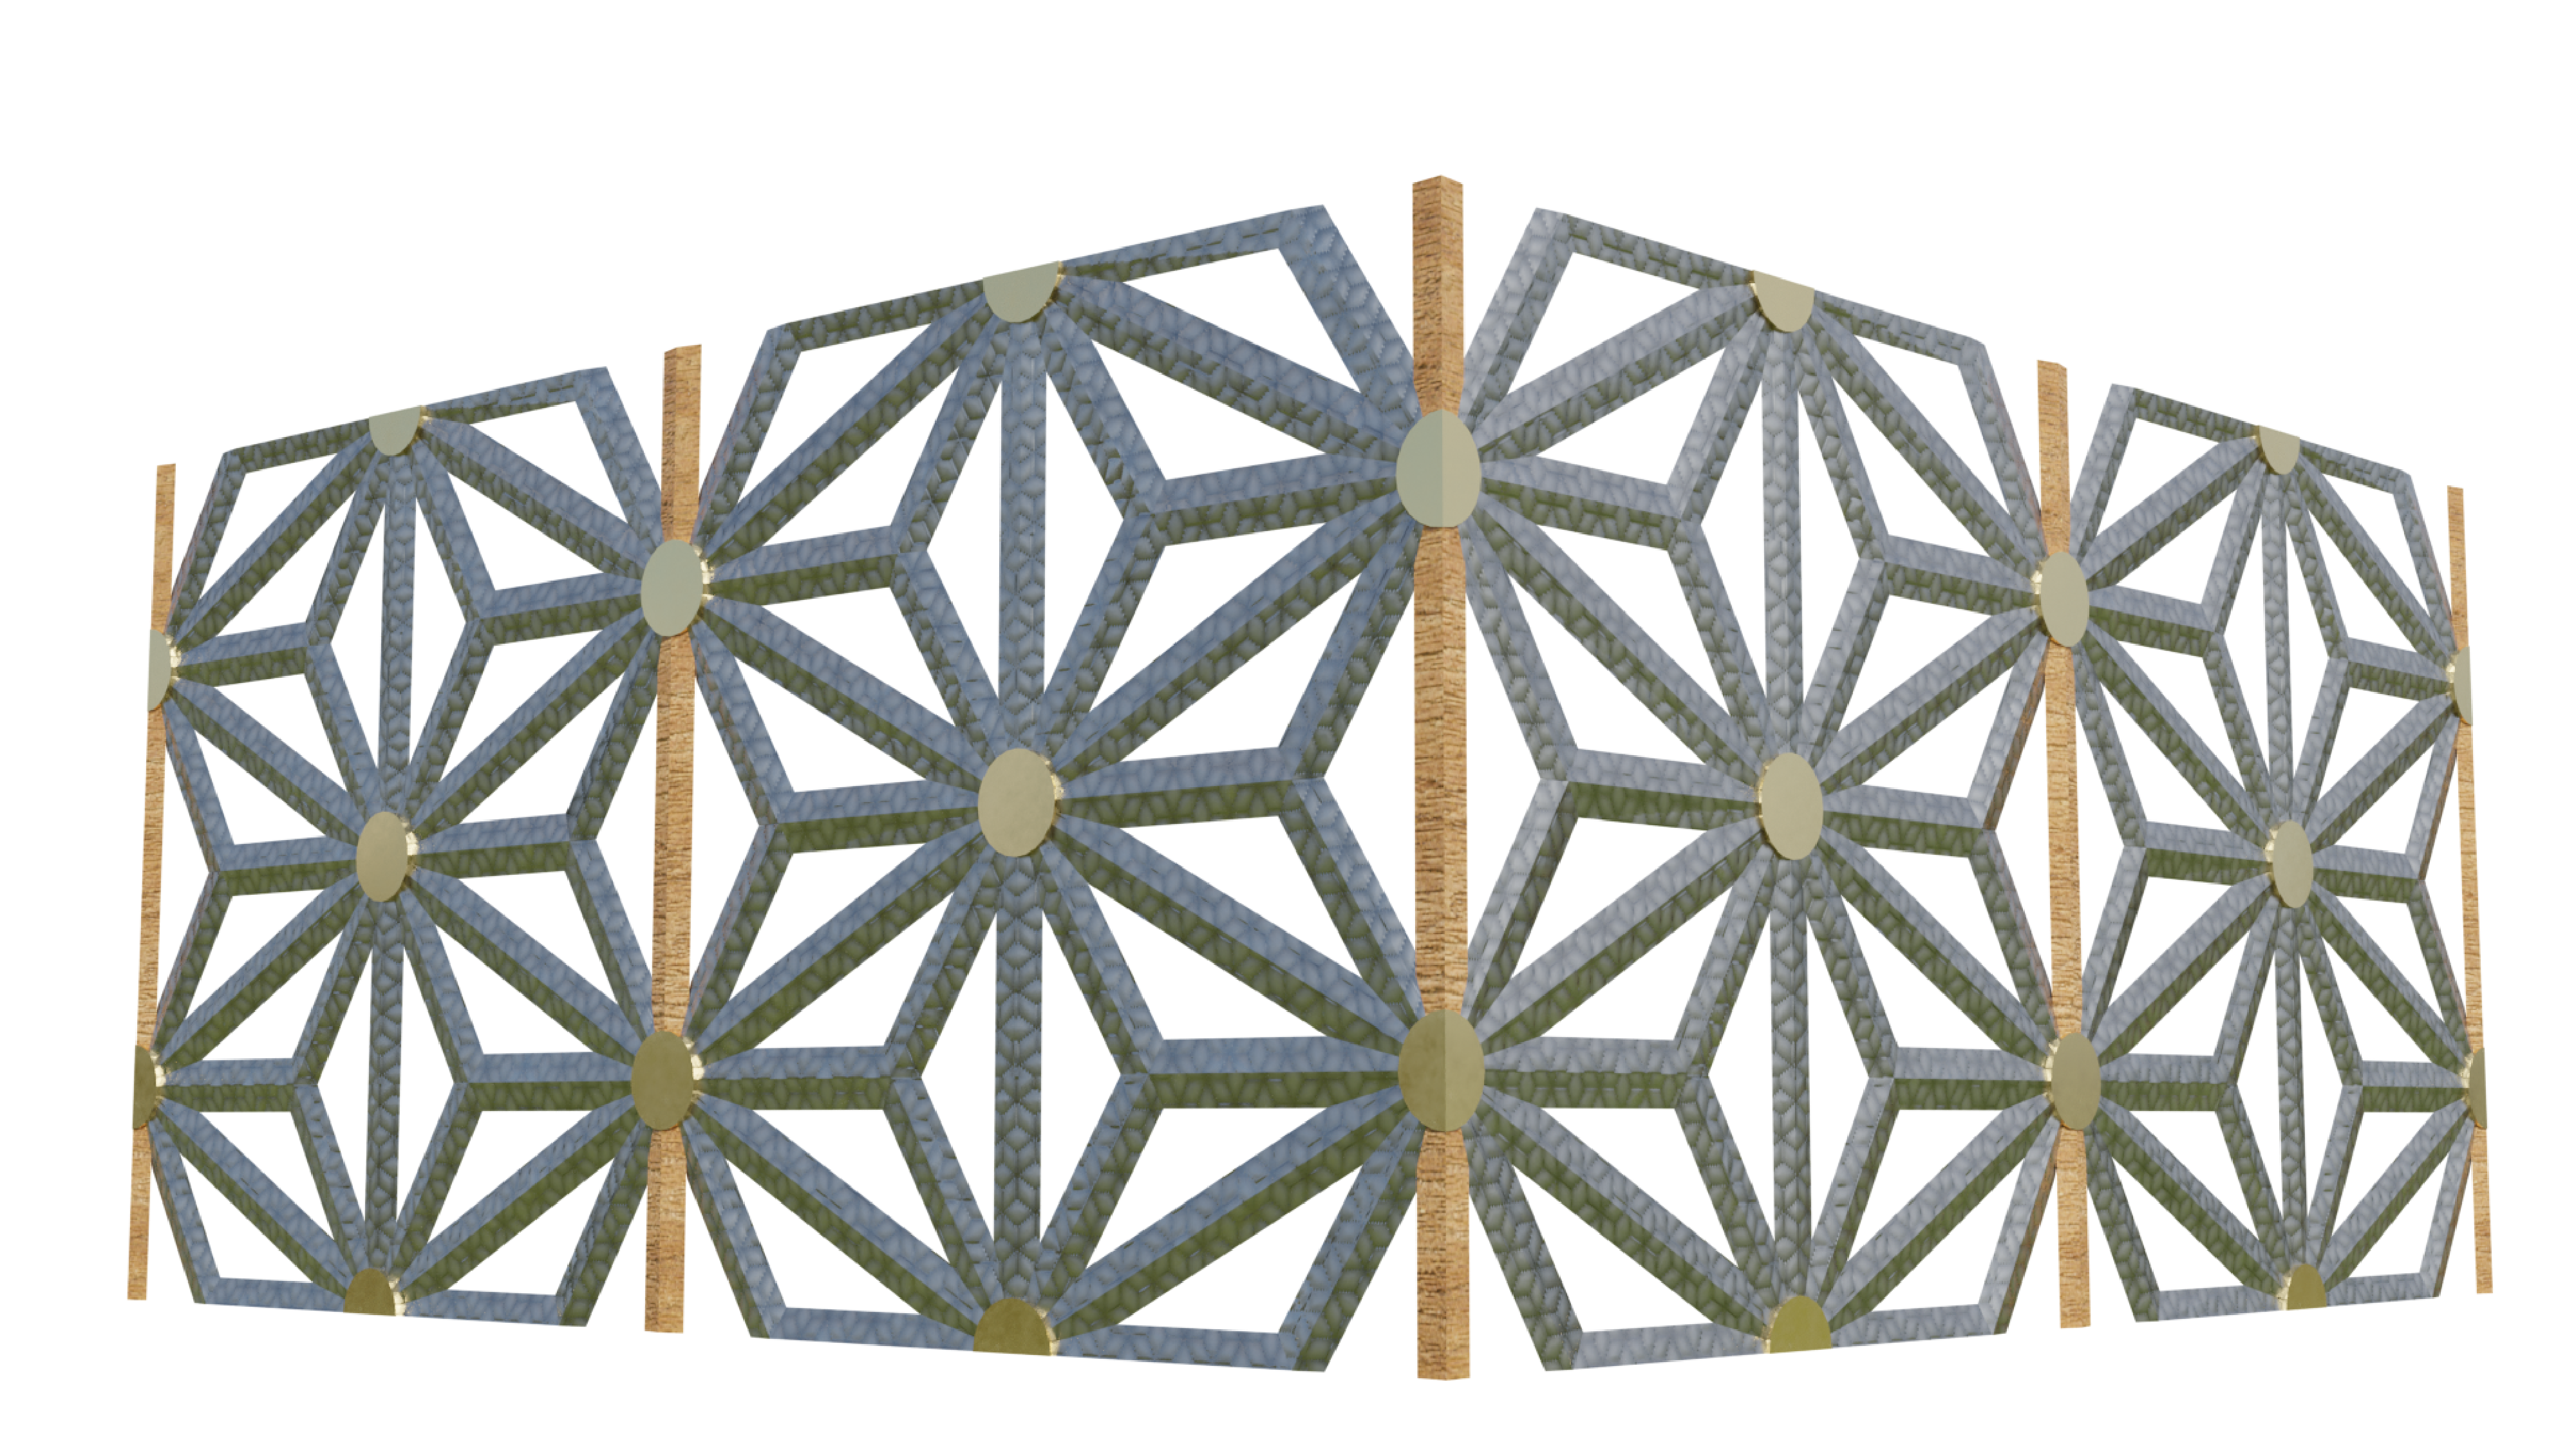
\includegraphics[width=1\linewidth]{Images/Base Module/Pattern3}} \\
            \midrule

            \textit{Mesh complexity Level} &
              \textit{Pattern 1} &
              \textit{Pattern 2} &
              \textit{Pattern 3}\\

            \midrule
            \textit{Level 6} &  &  &
            \\
            {\includegraphics[width=1\linewidth]{Images/Wall 0/0006}} &
                {\includegraphics[width=1\linewidth]{Images/Pattern 1/0006}} &
              {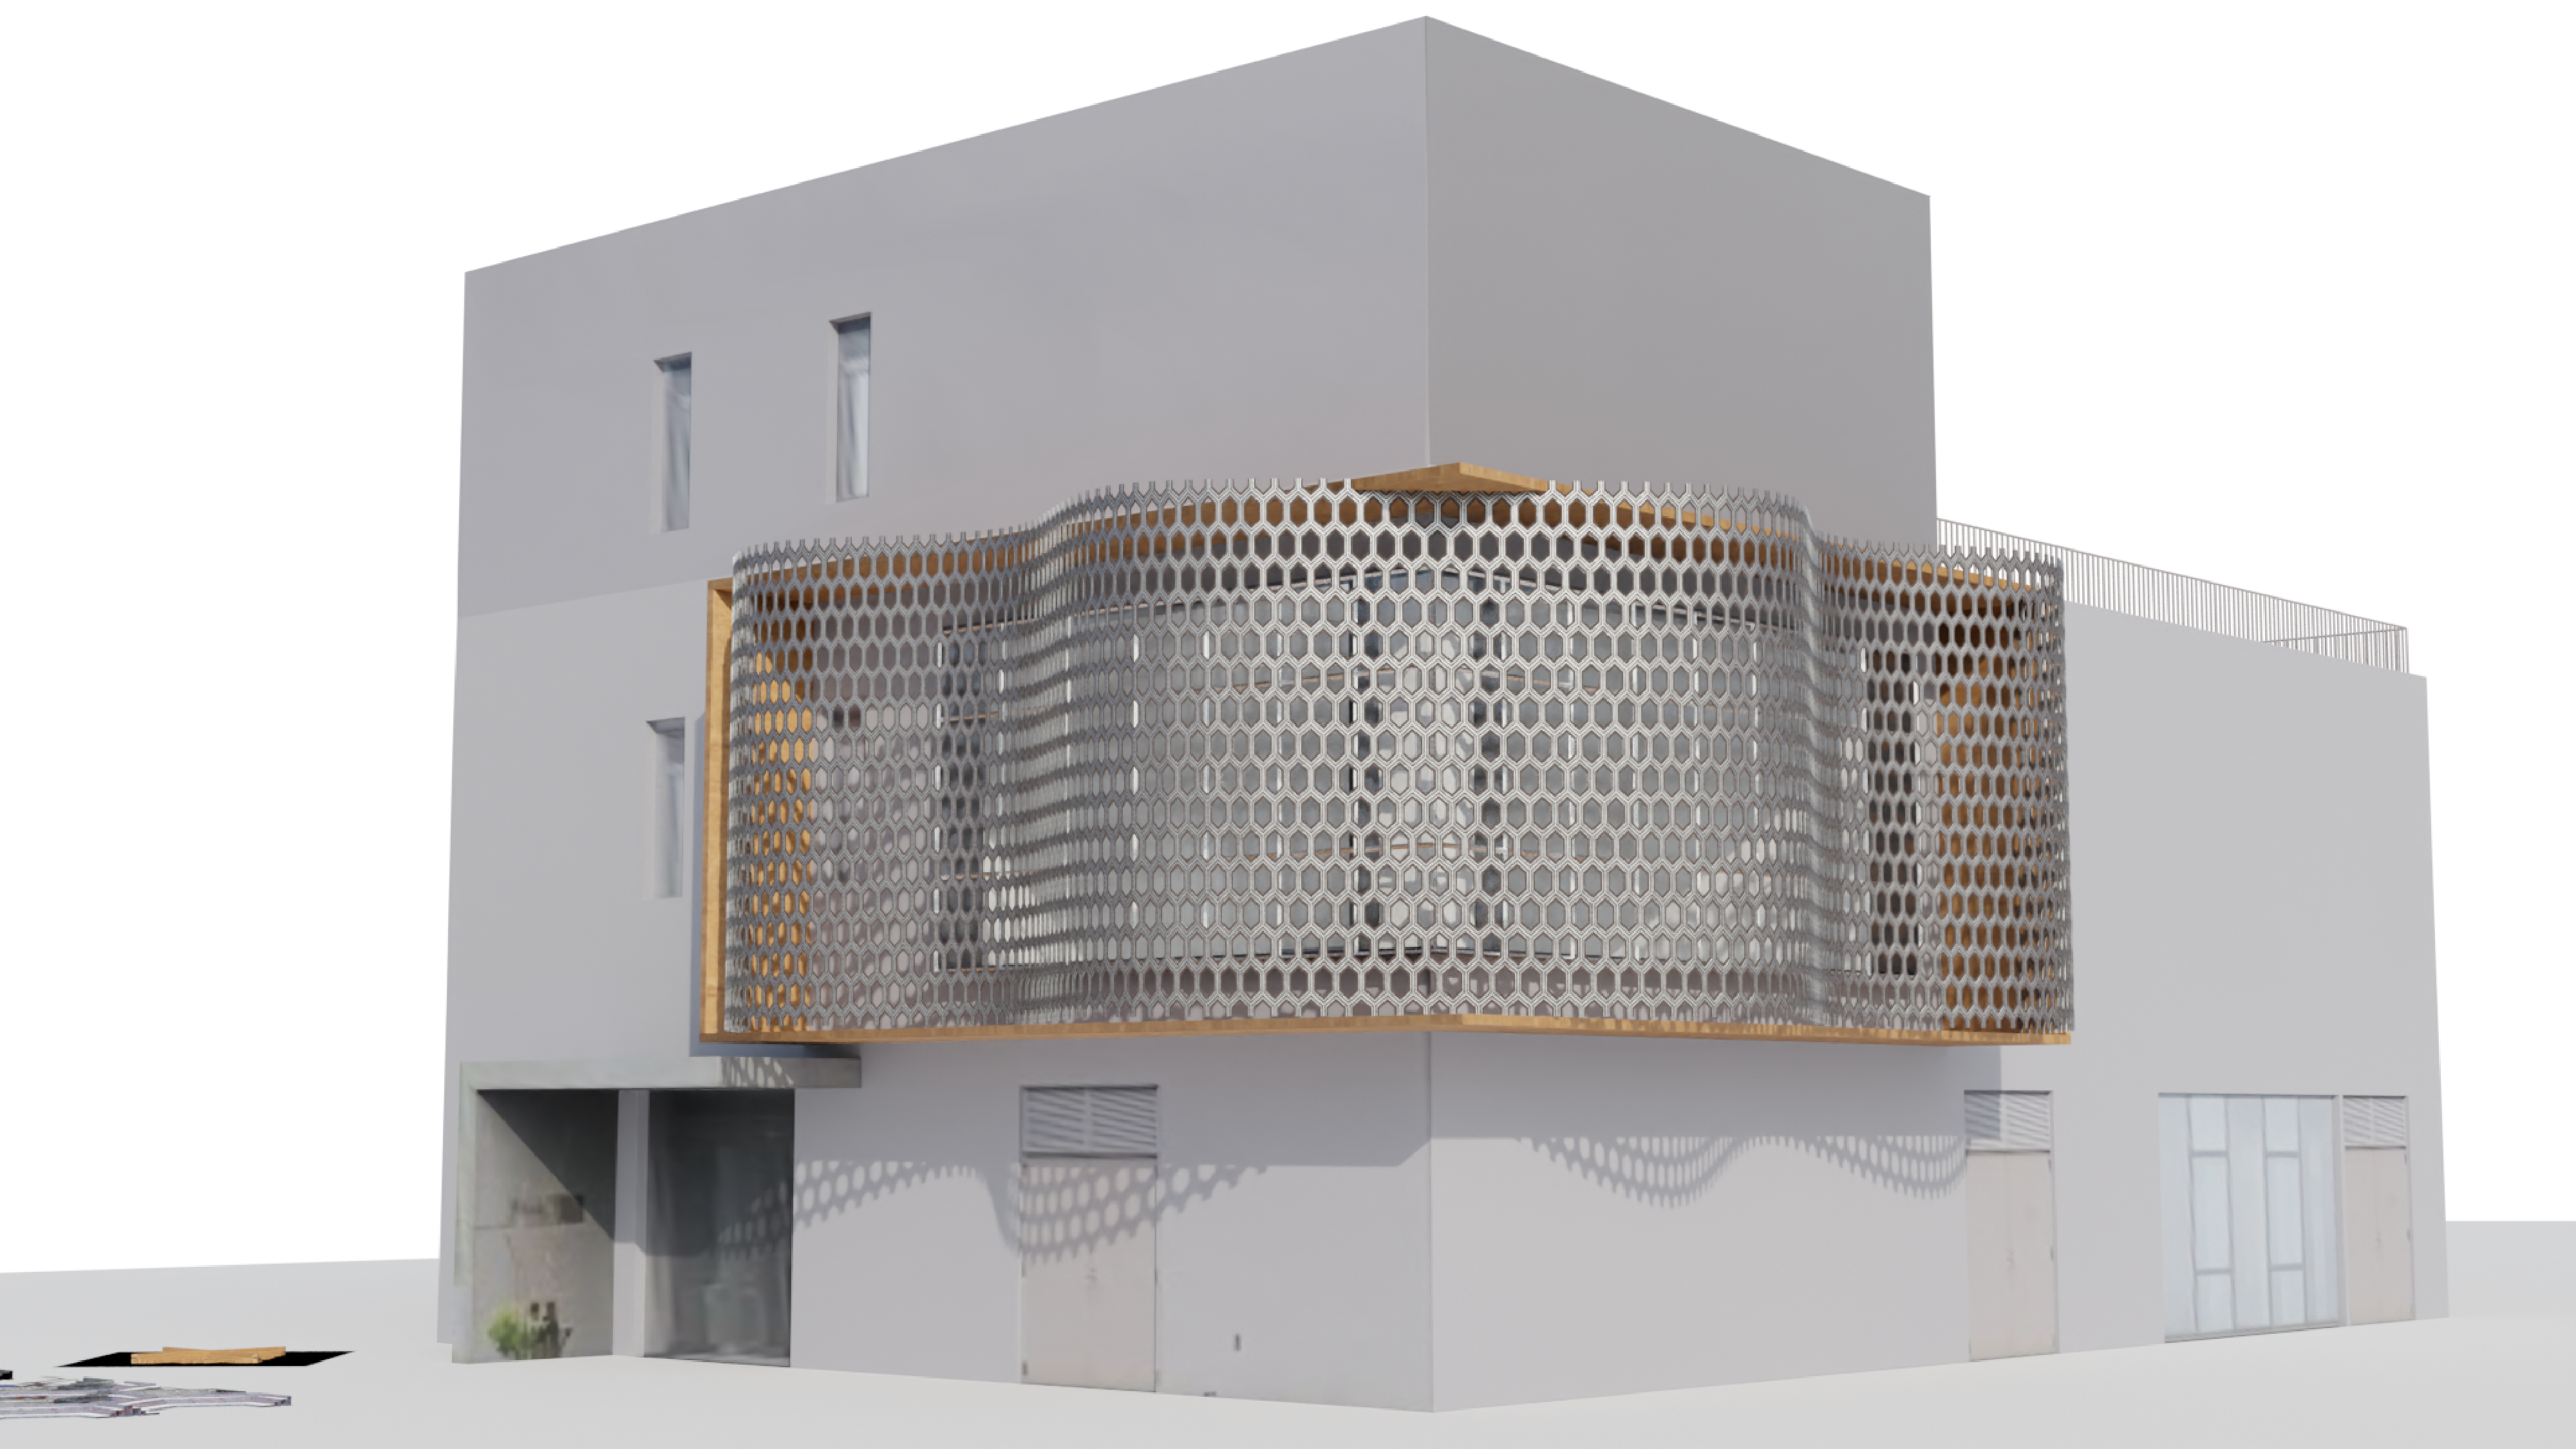
\includegraphics[width=1\linewidth]{Images/Pattern 2/0006}} &
              {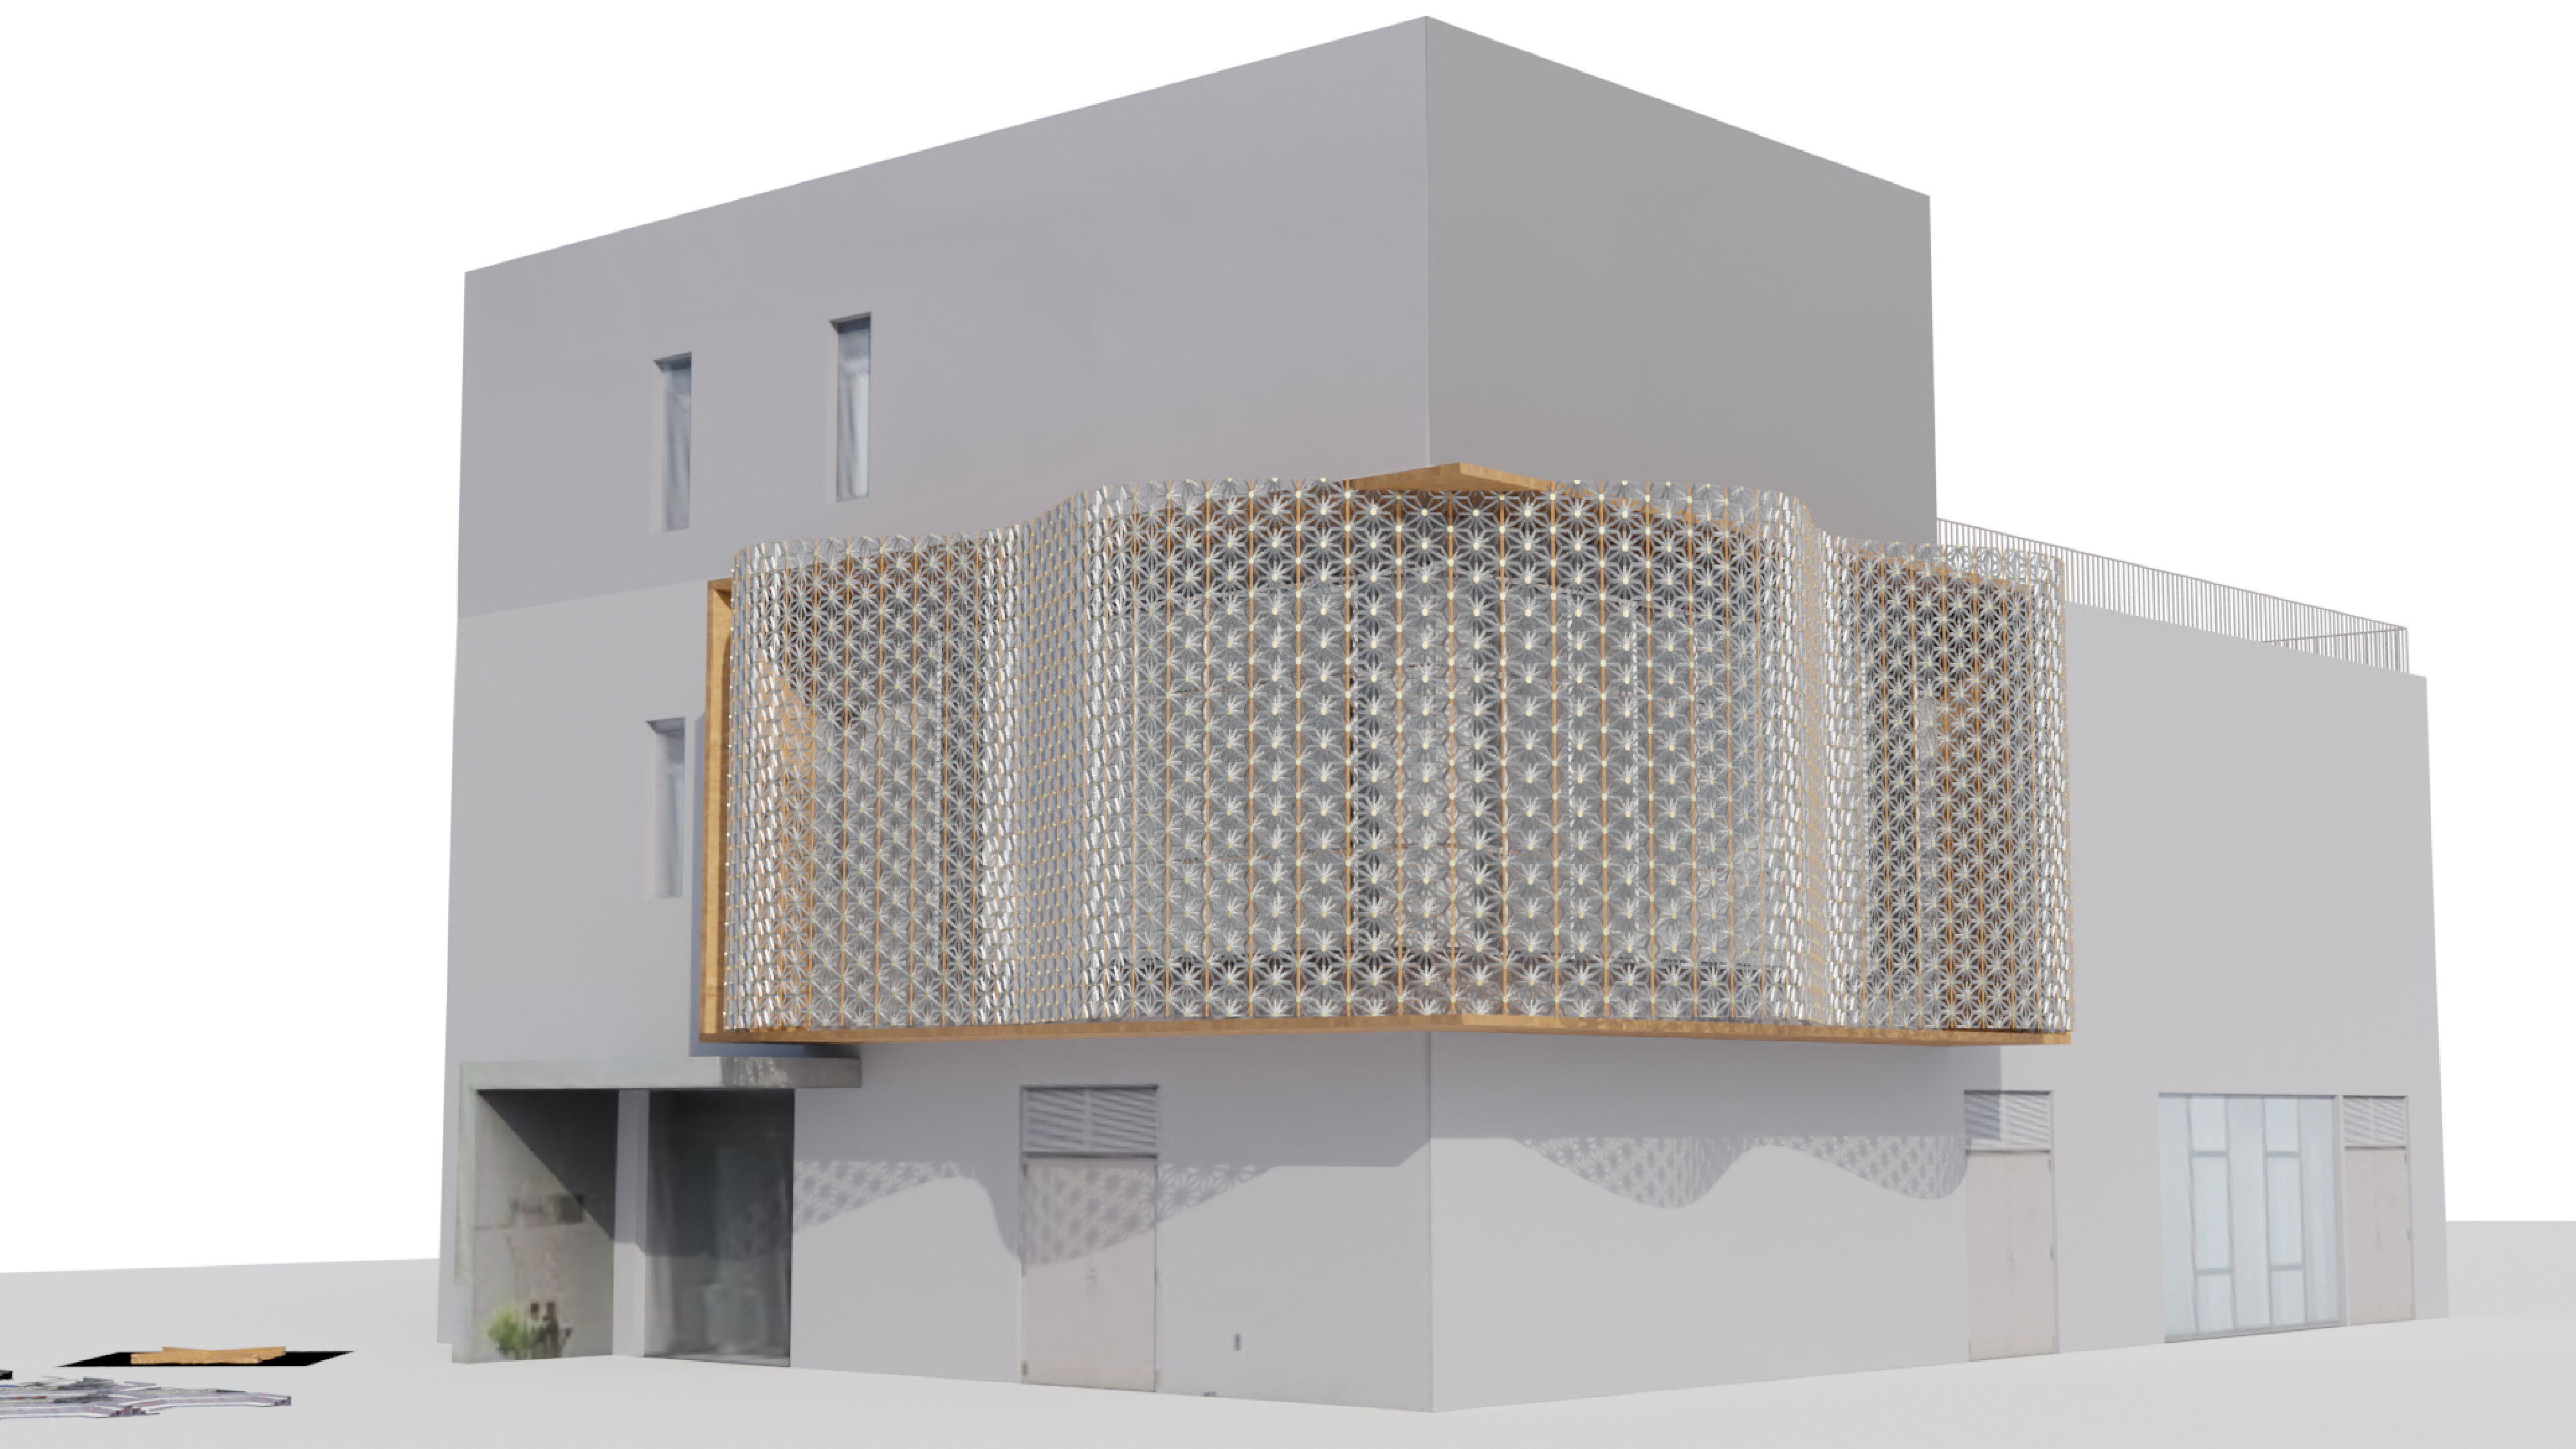
\includegraphics[width=1\linewidth]{Images/Pattern 3/0006}}\\
            \midrule
            \textit{Level 7} &  &  &
            \\
            {\includegraphics[width=1\linewidth]{Images/Wall 0/0007}} &
              {\includegraphics[width=1\linewidth]{Images/Pattern 1/0007}} &
              {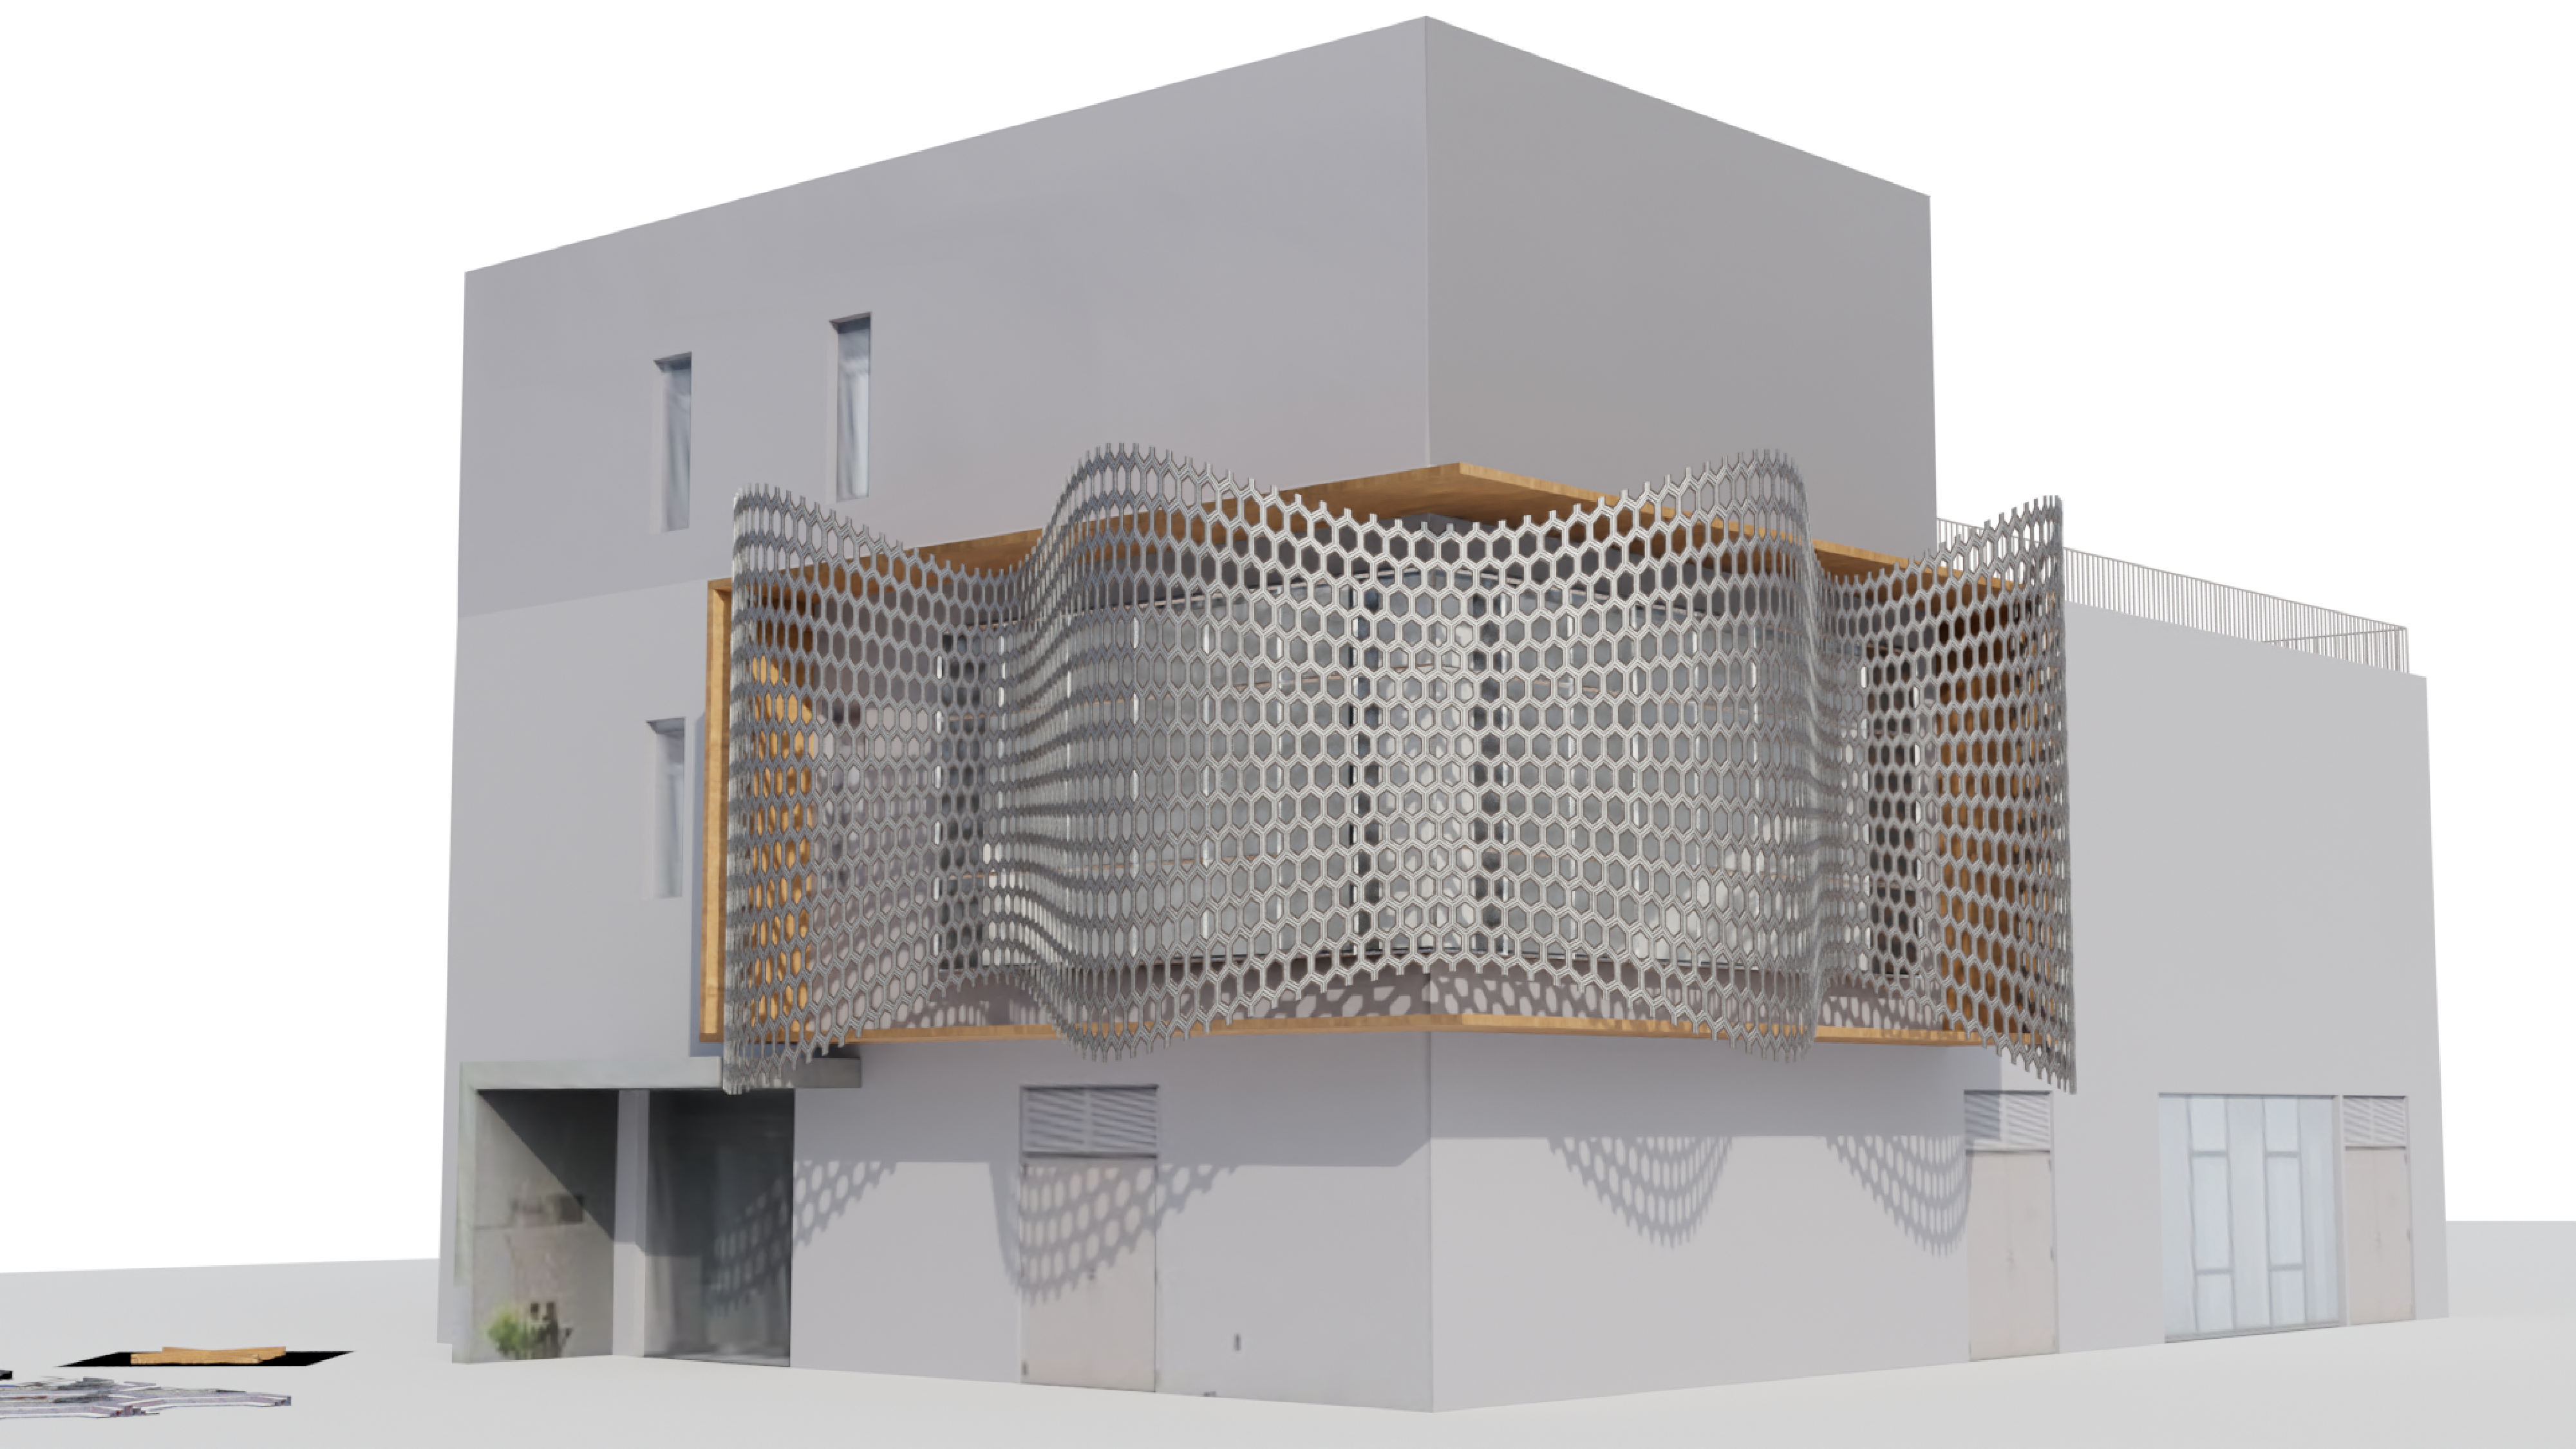
\includegraphics[width=1\linewidth]{Images/Pattern 2/0007}} &
              {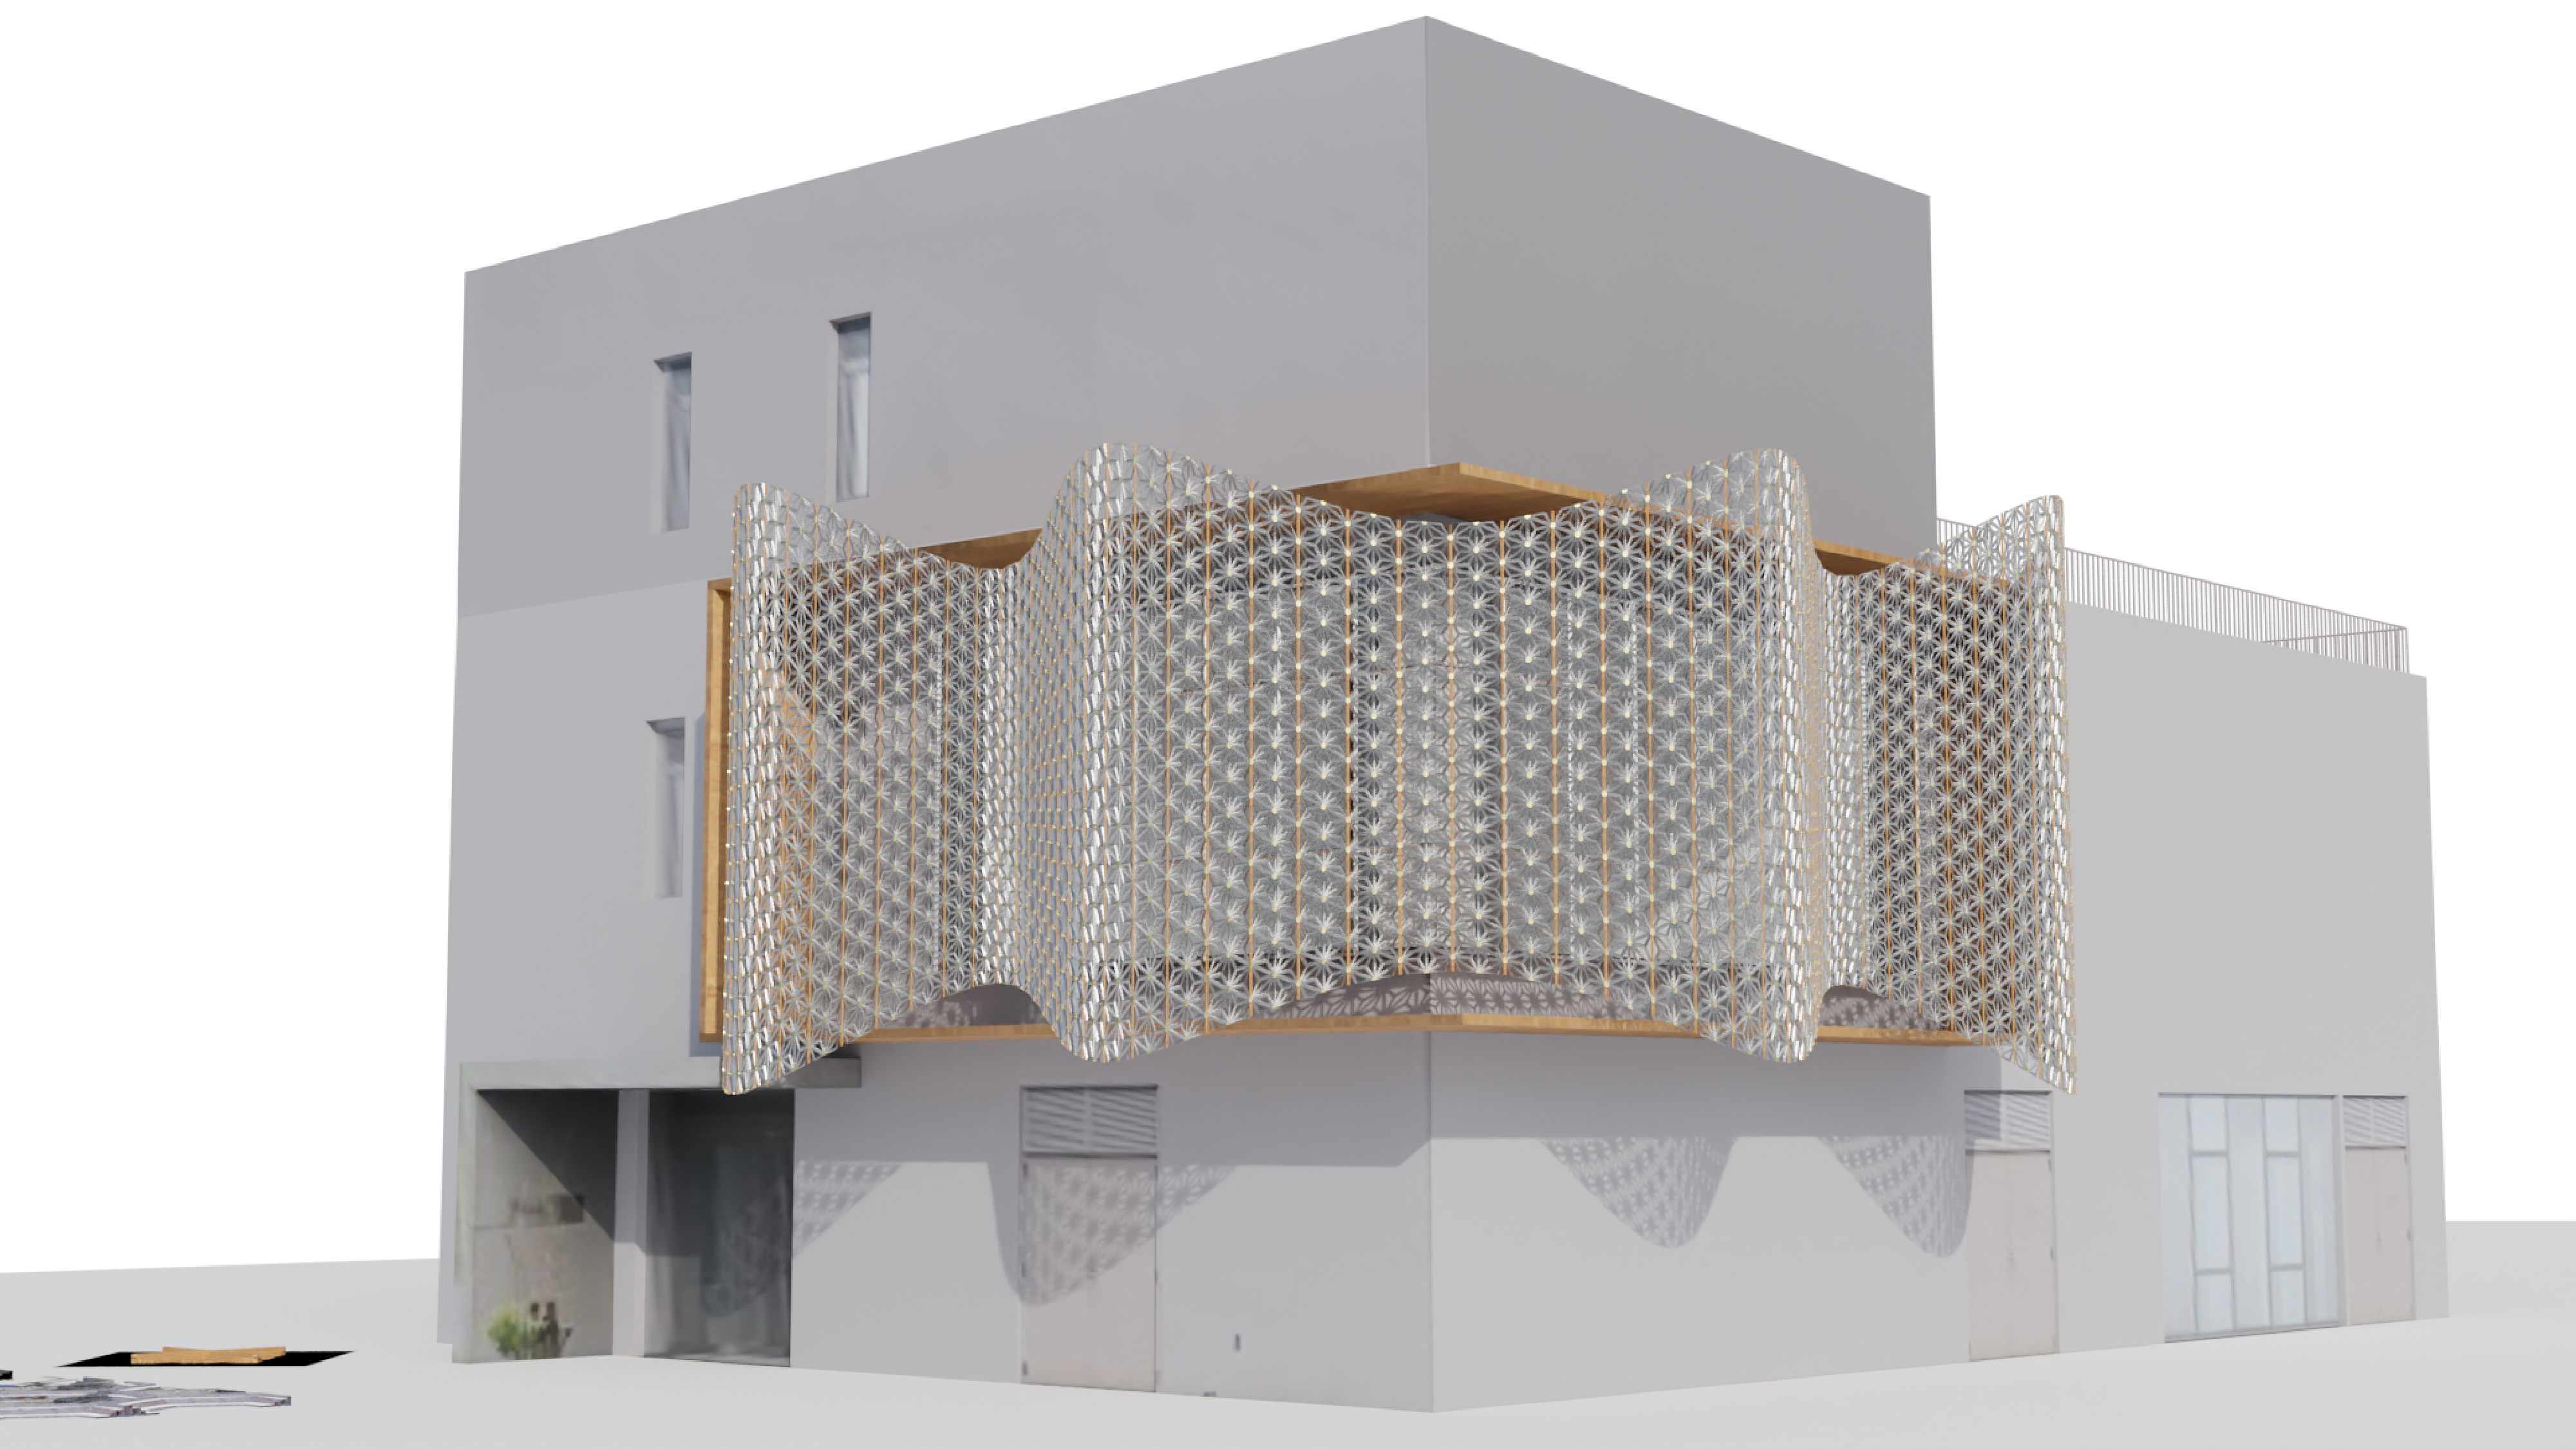
\includegraphics[width=1\linewidth]{Images/Pattern 3/0007}} \\
            \midrule
            \textit{Level 8} &  &  &
            \\
            {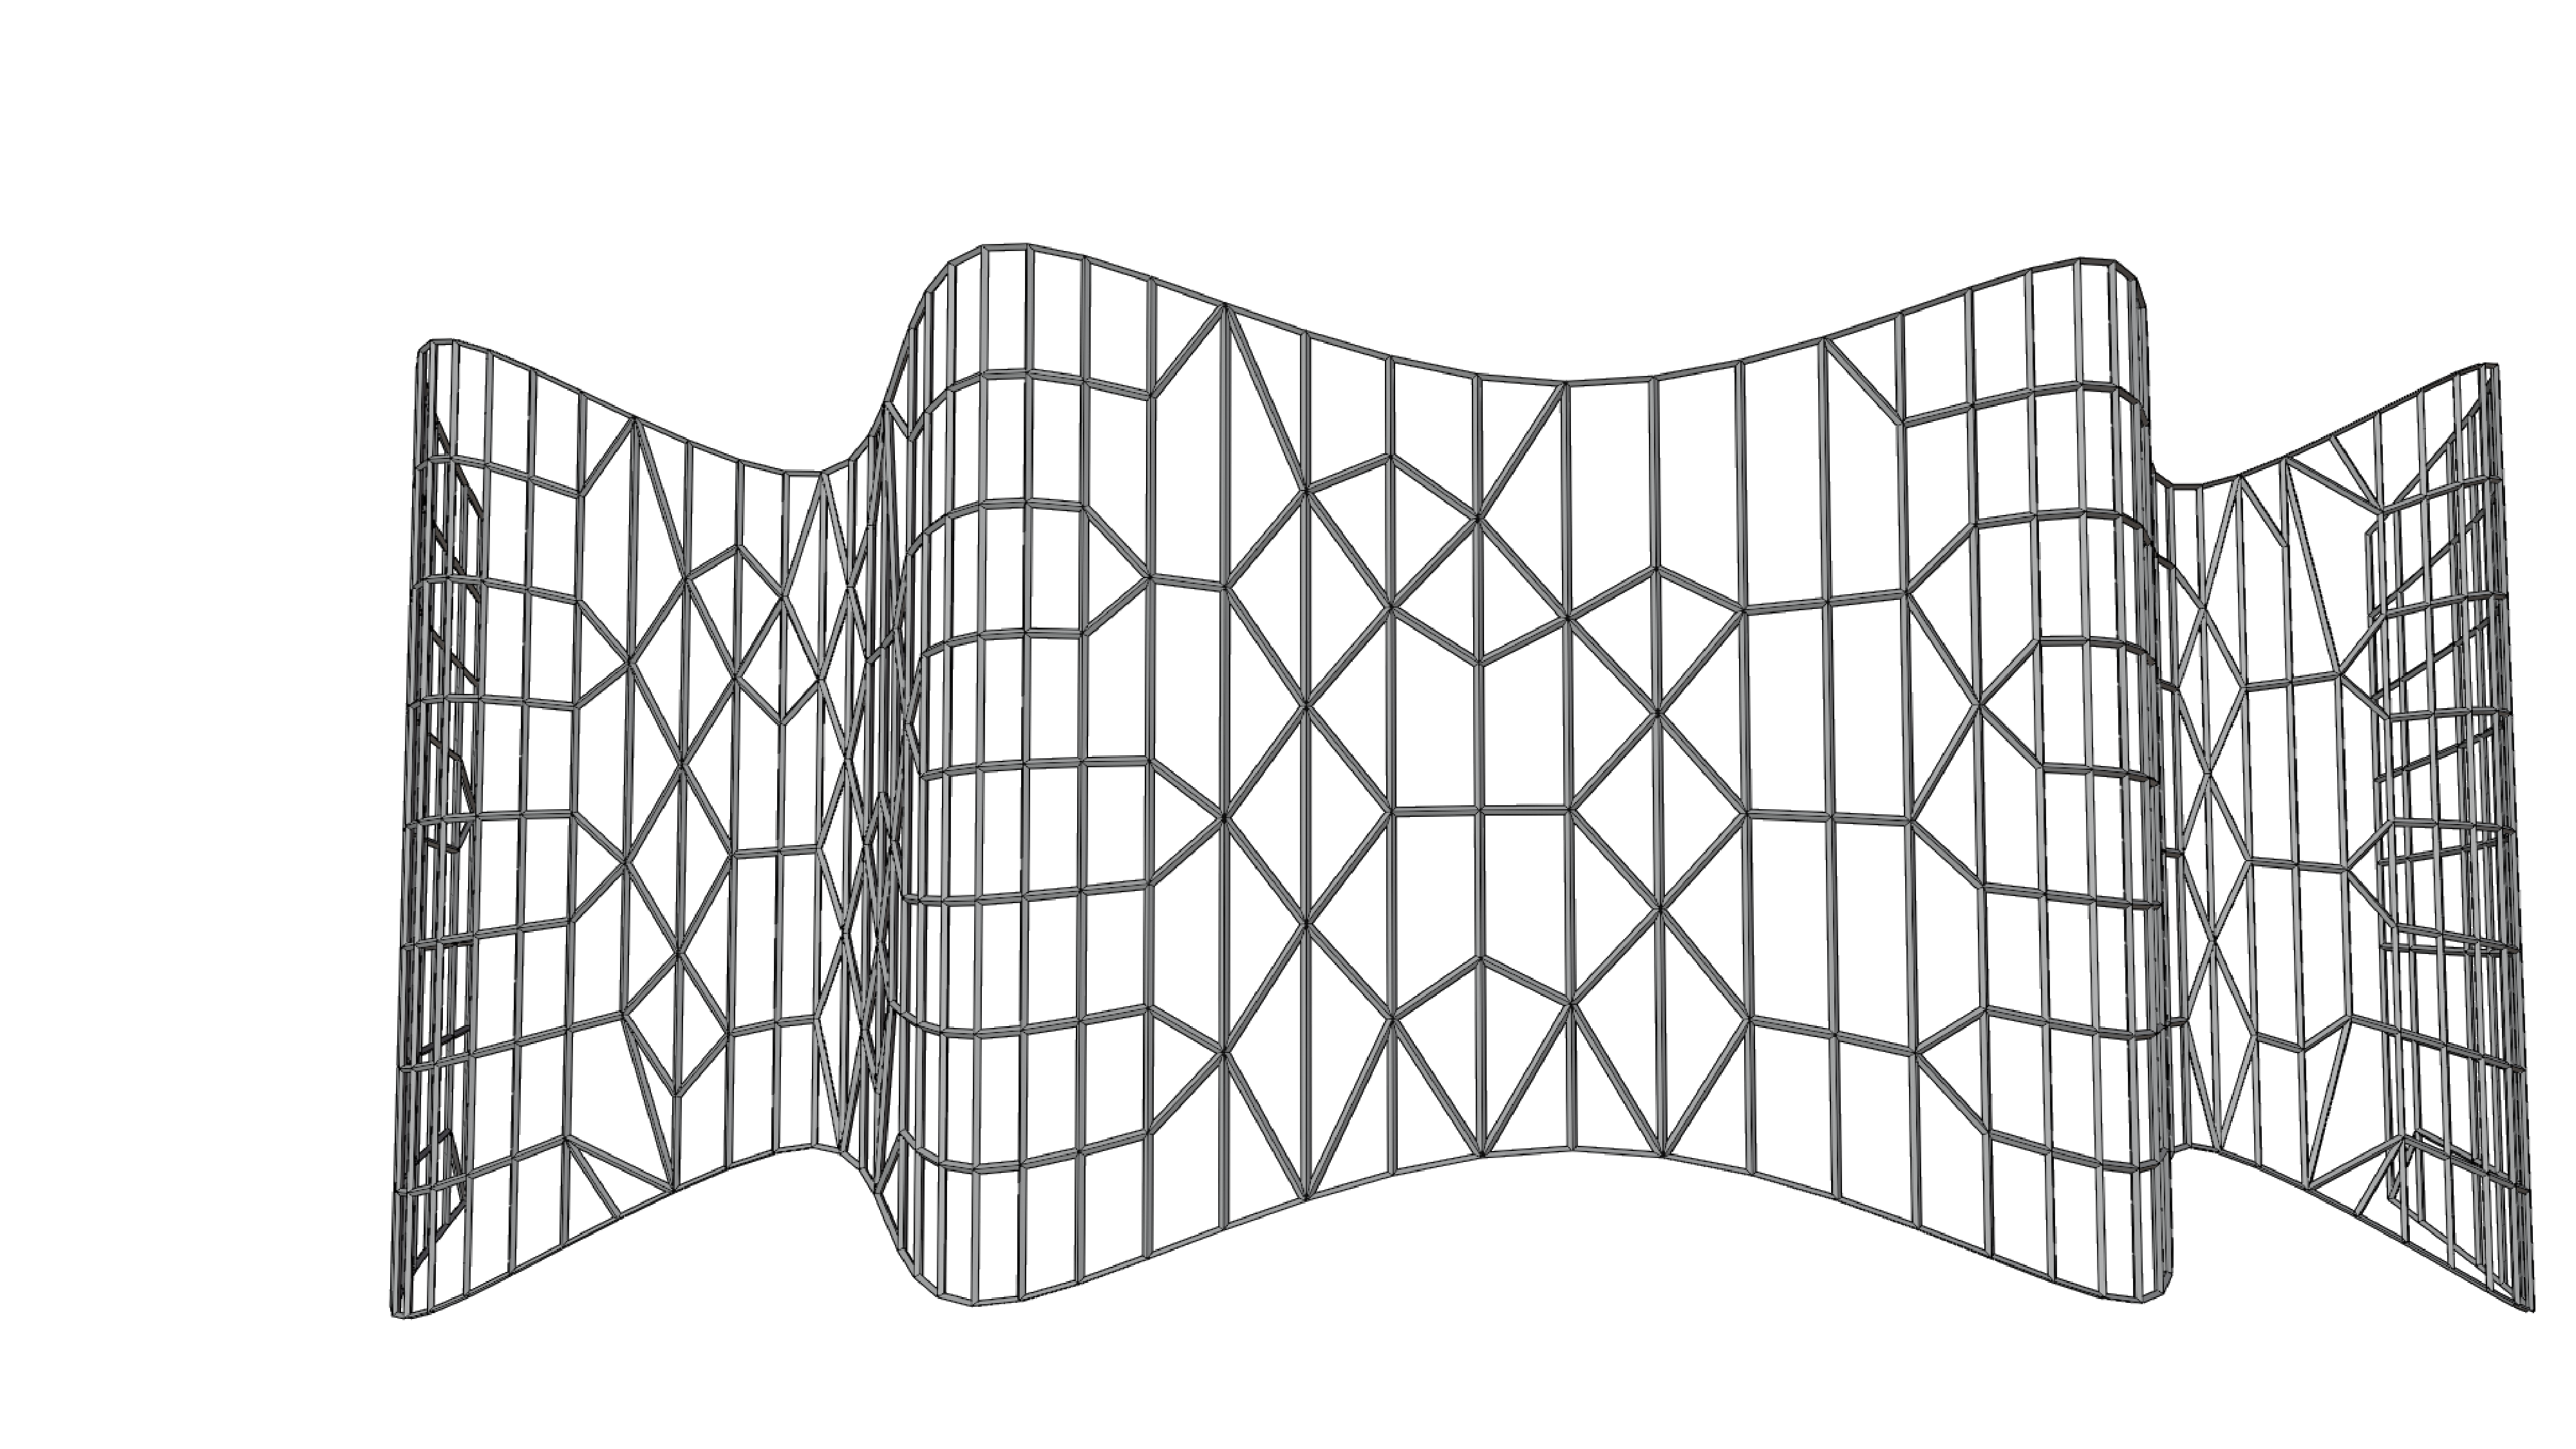
\includegraphics[width=1\linewidth]{Images/Wall 0/0008}} &
              {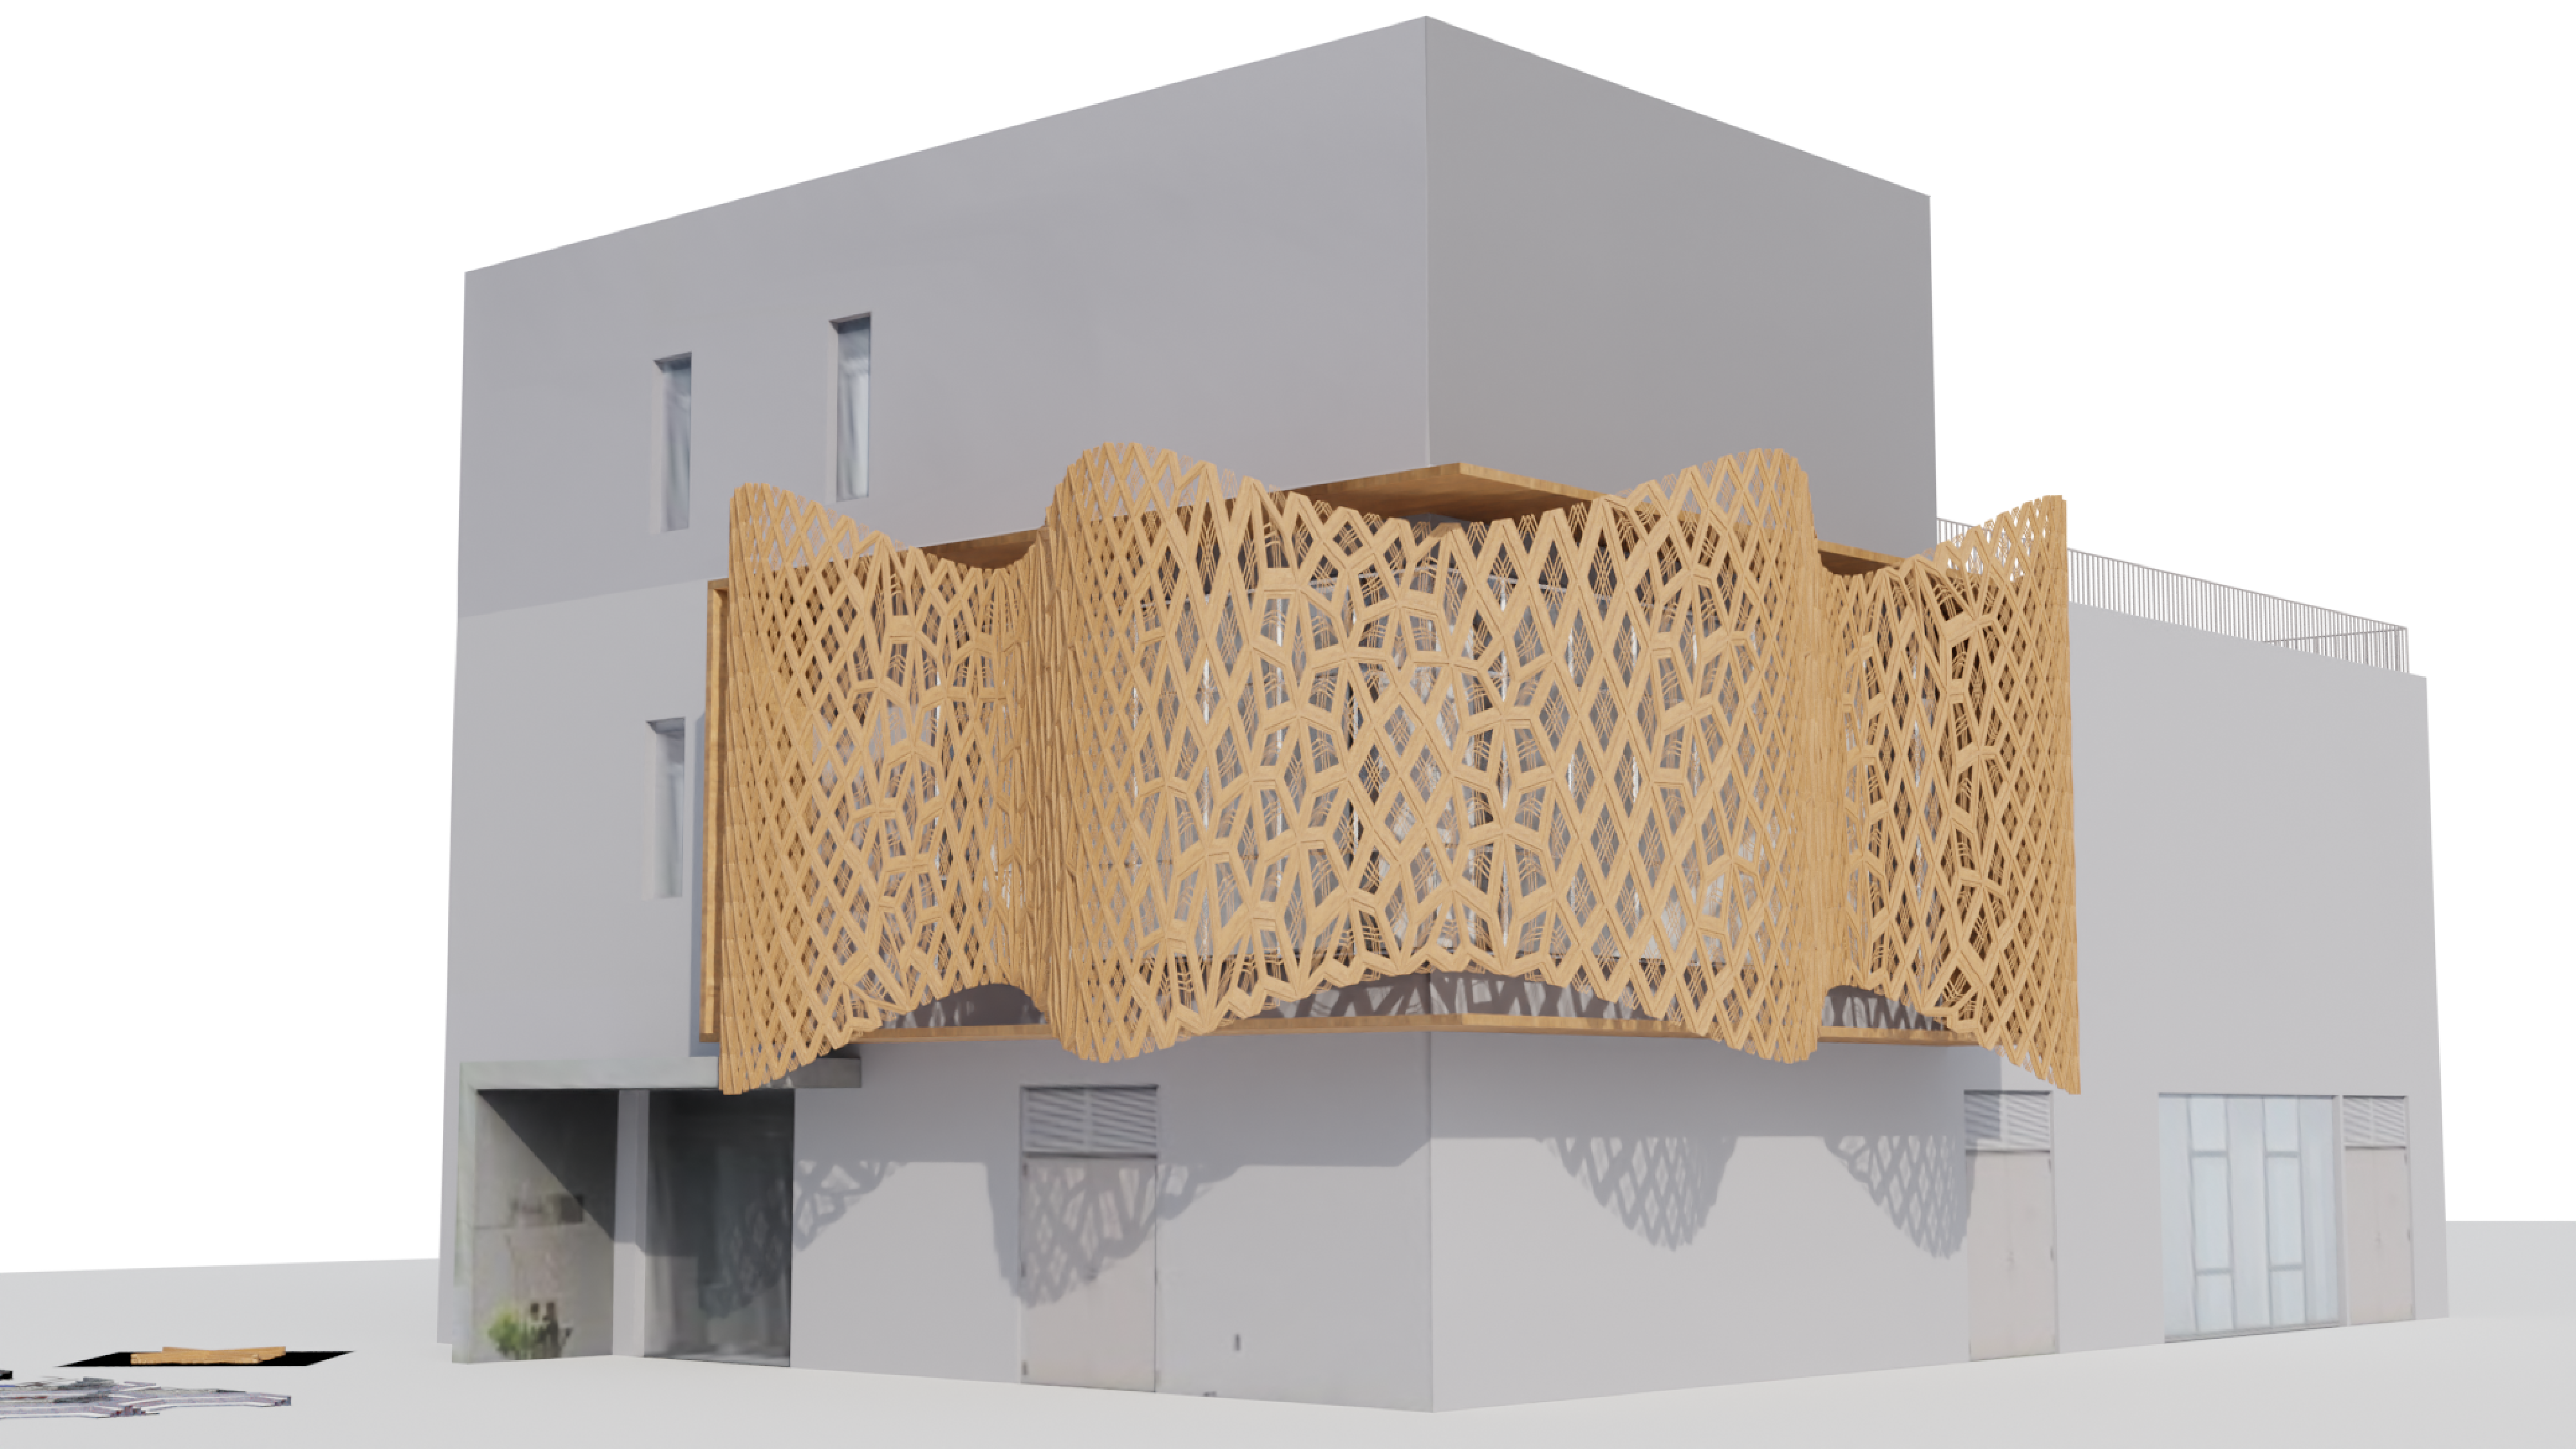
\includegraphics[width=1\linewidth]{Images/Pattern 1/0008}} &
              {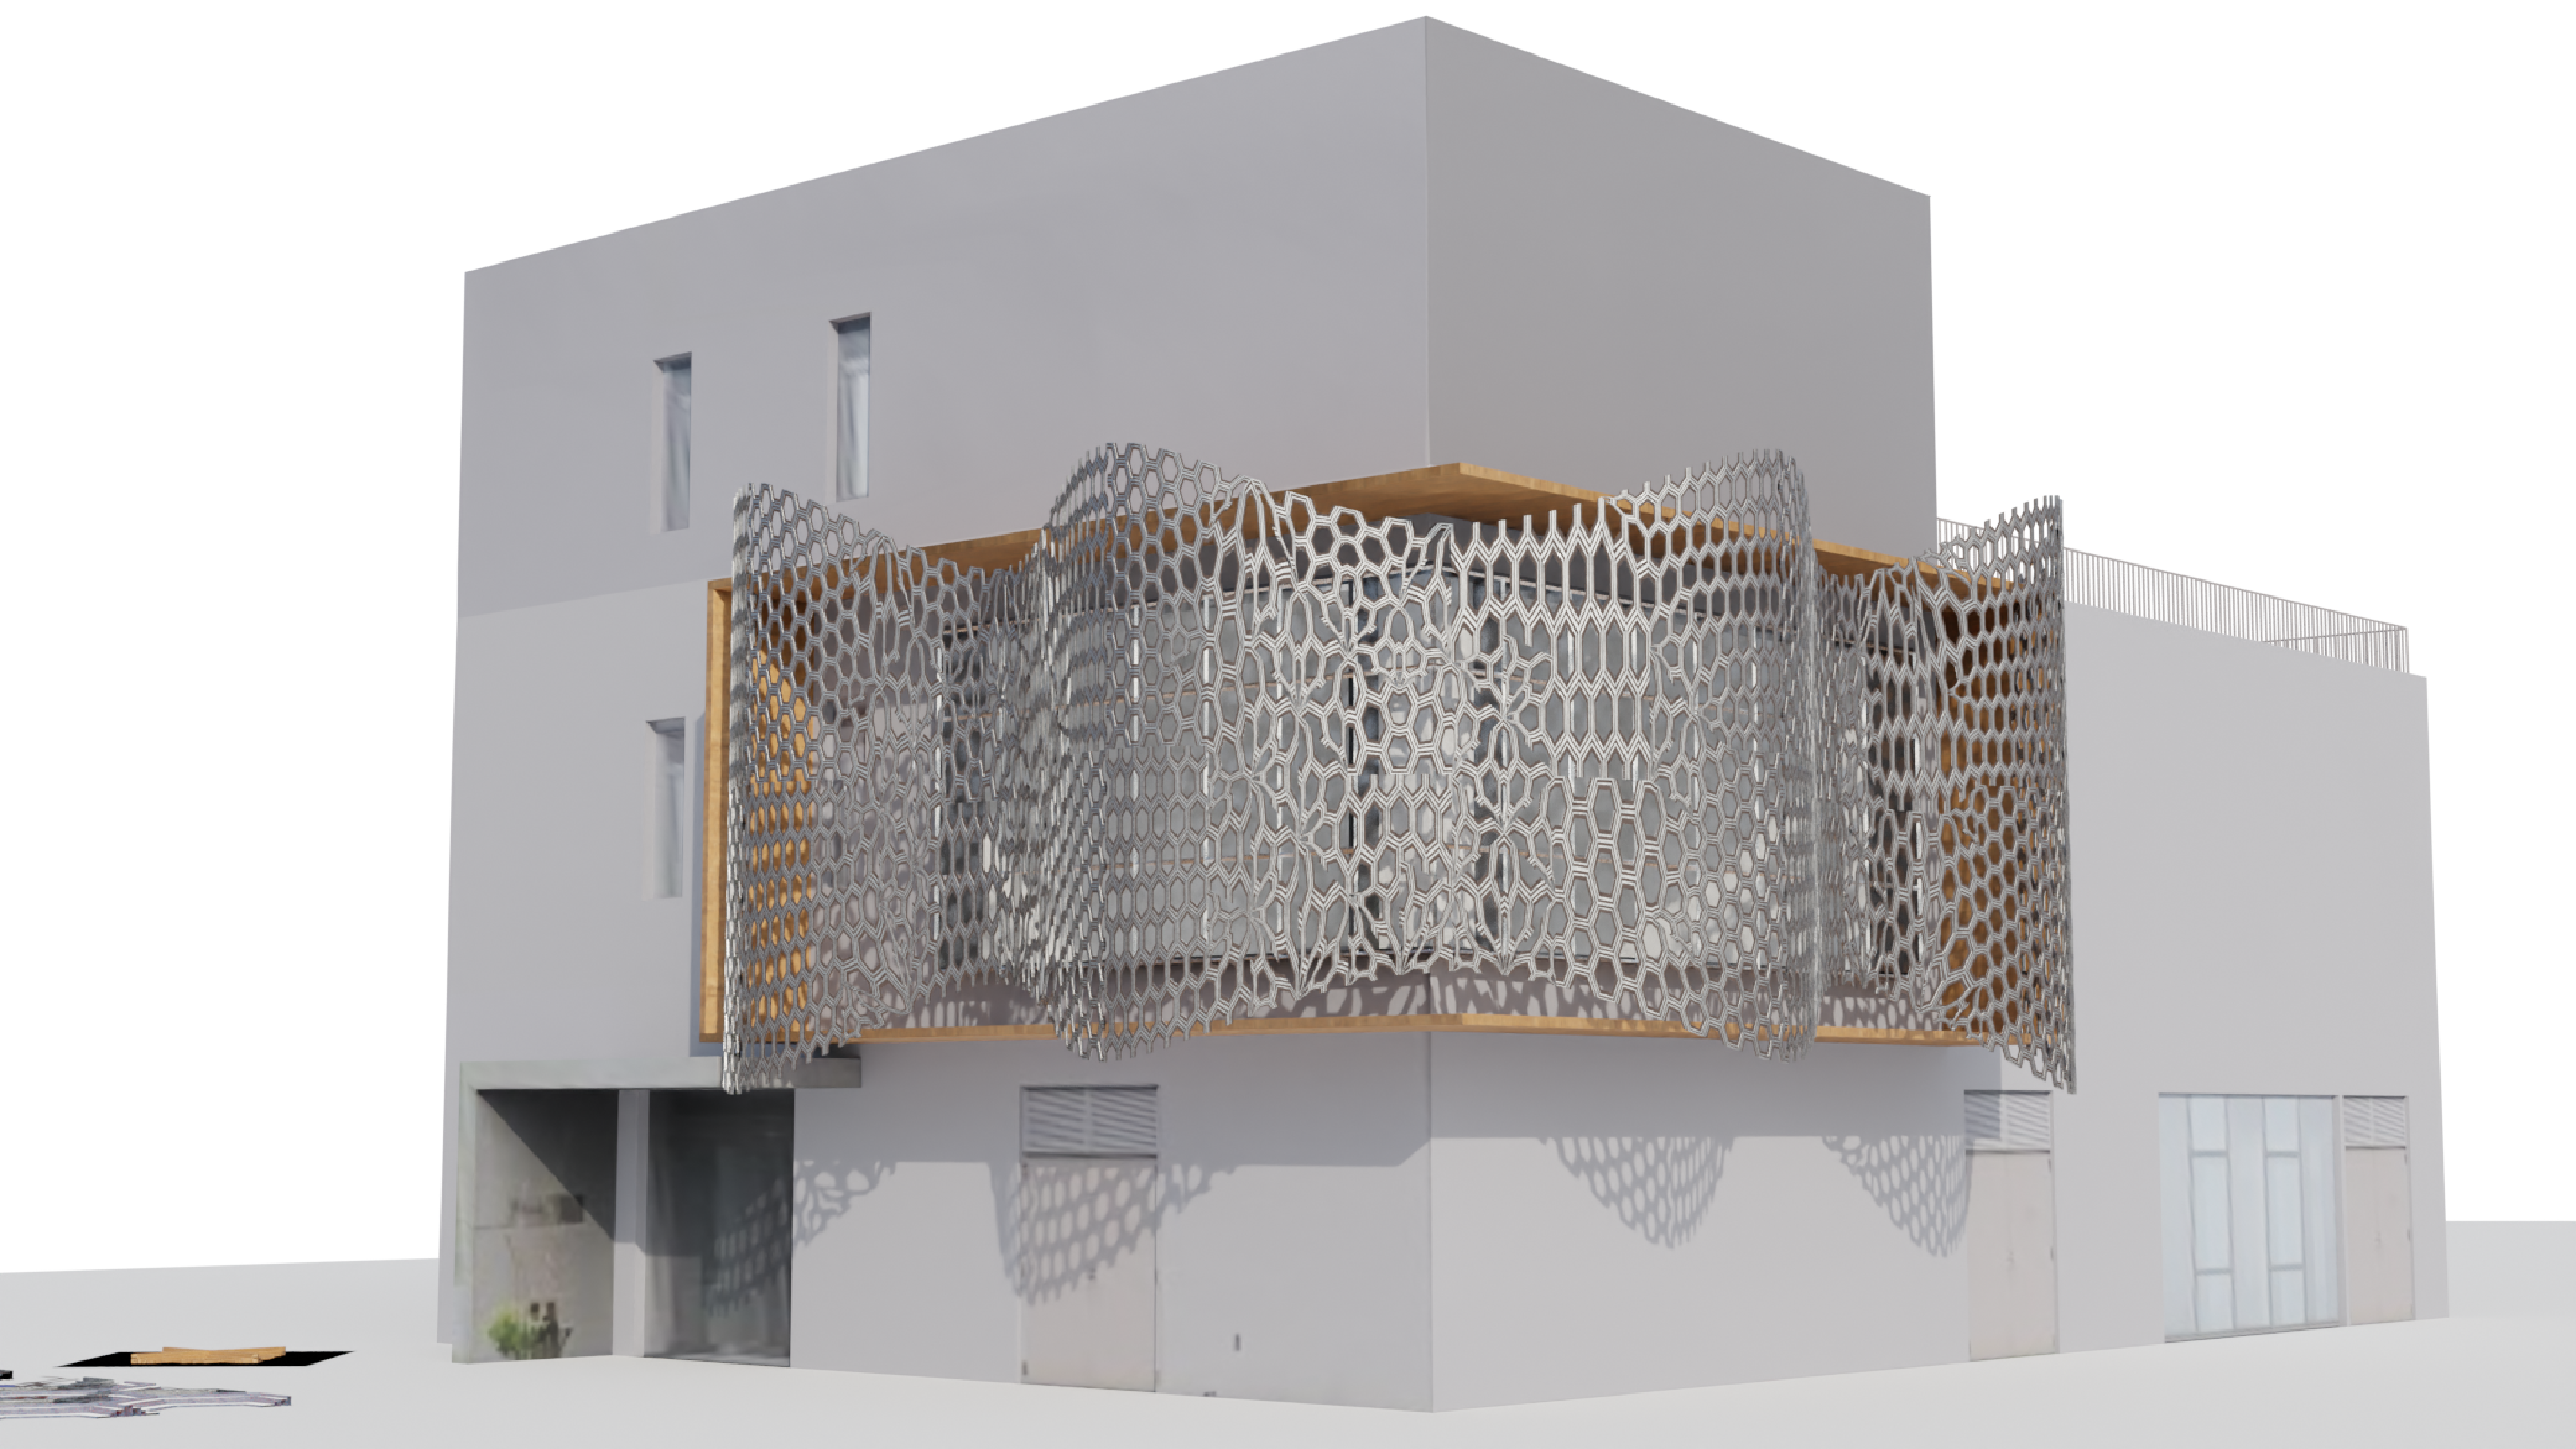
\includegraphics[width=1\linewidth]{Images/Pattern 2/0008}} &
              {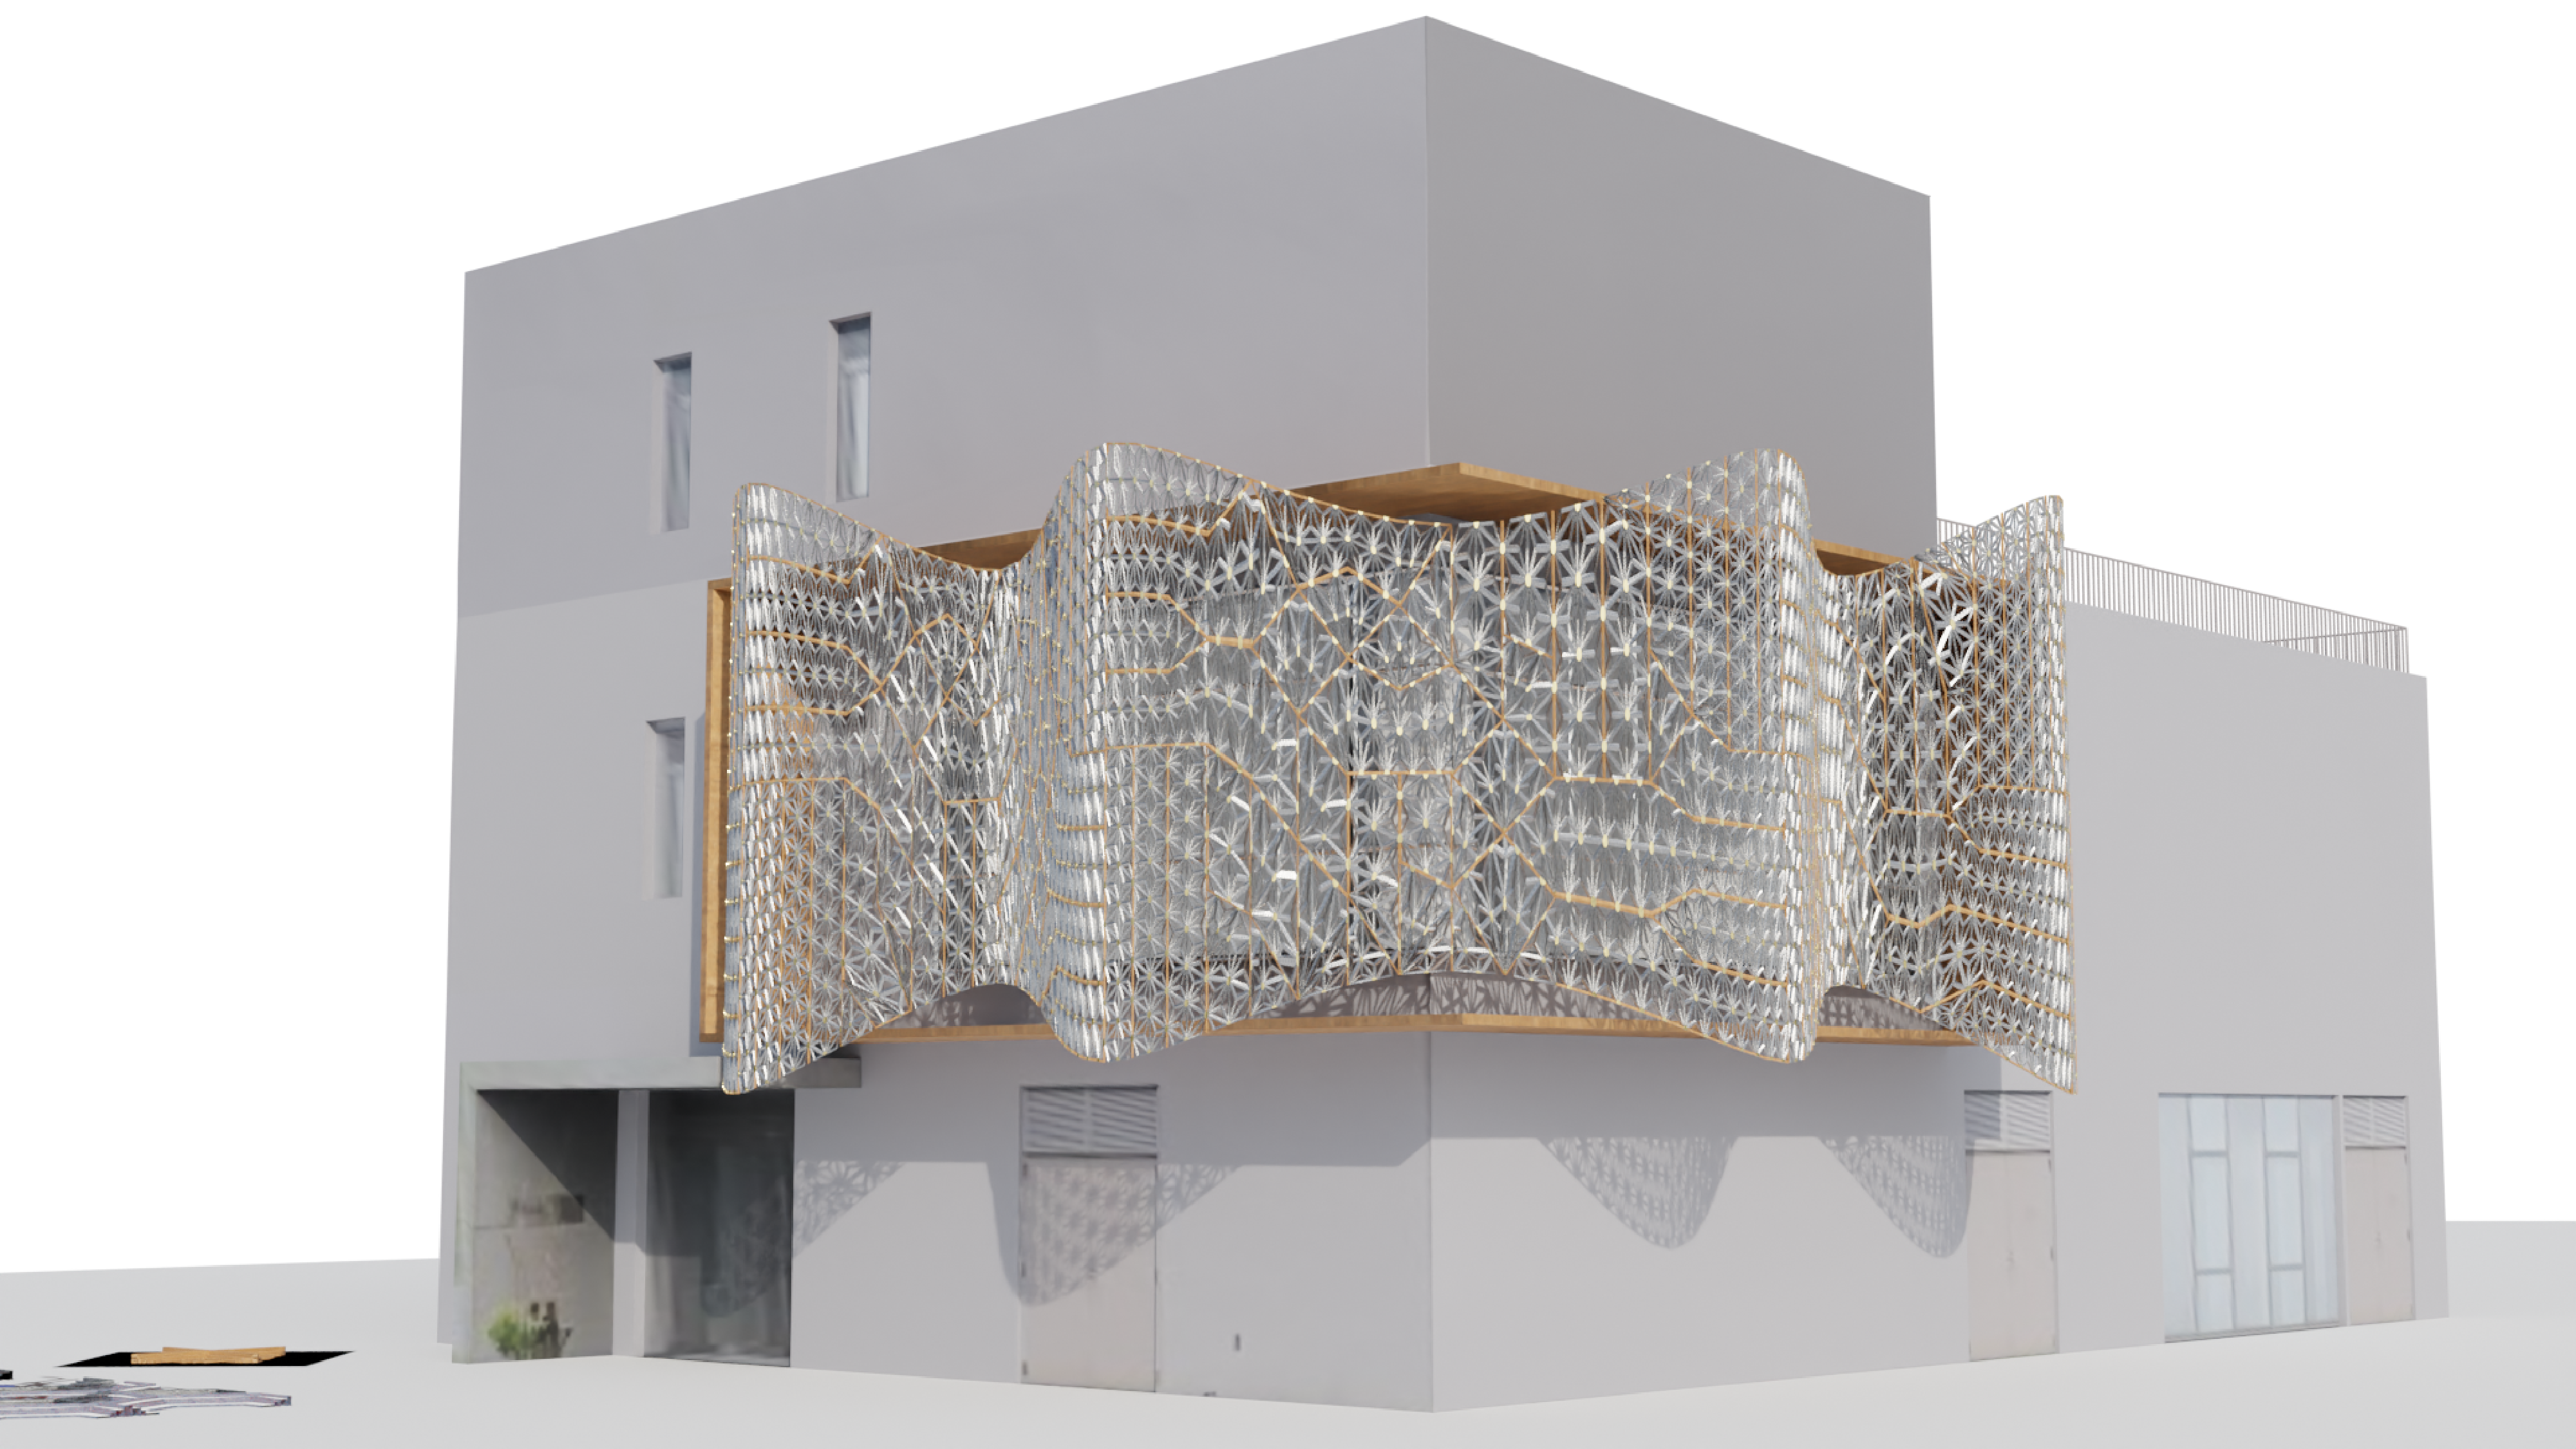
\includegraphics[width=1\linewidth]{Images/Pattern 3/0008}}\\
            \midrule
            \textit{Level 9} &  &  &
            \\
            {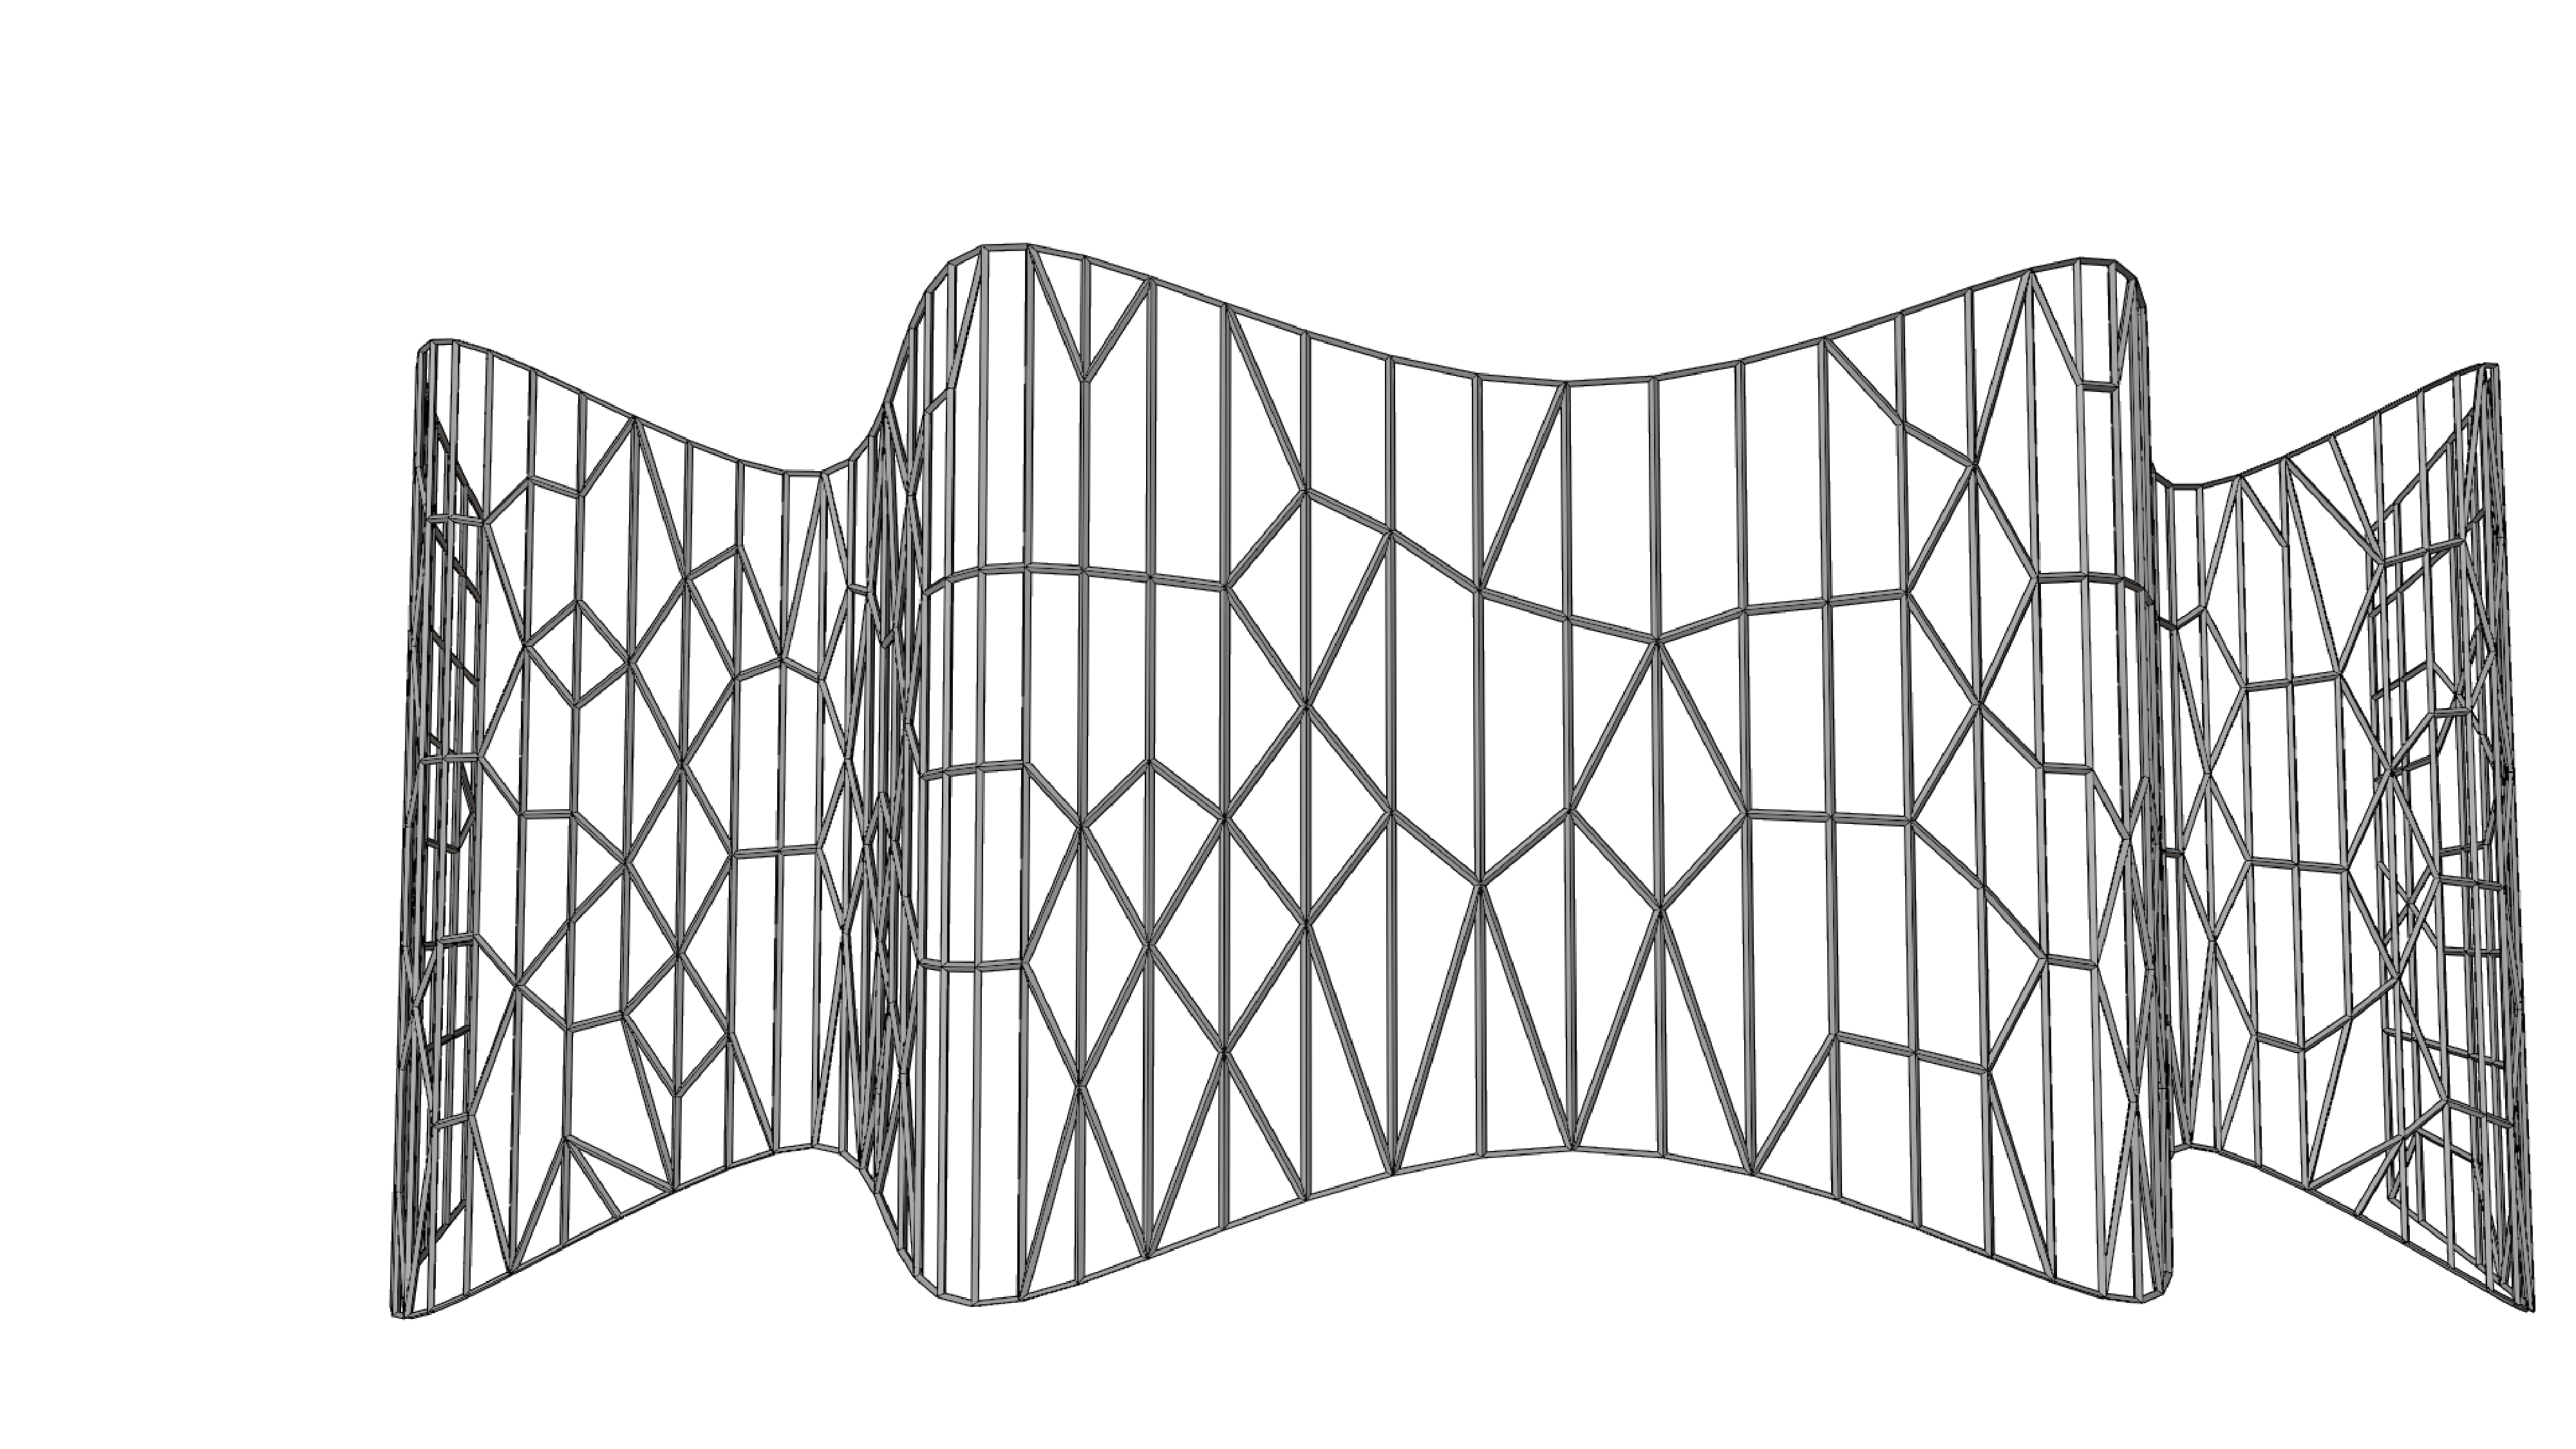
\includegraphics[width=1\linewidth]{Images/Wall 0/0009}} &
              {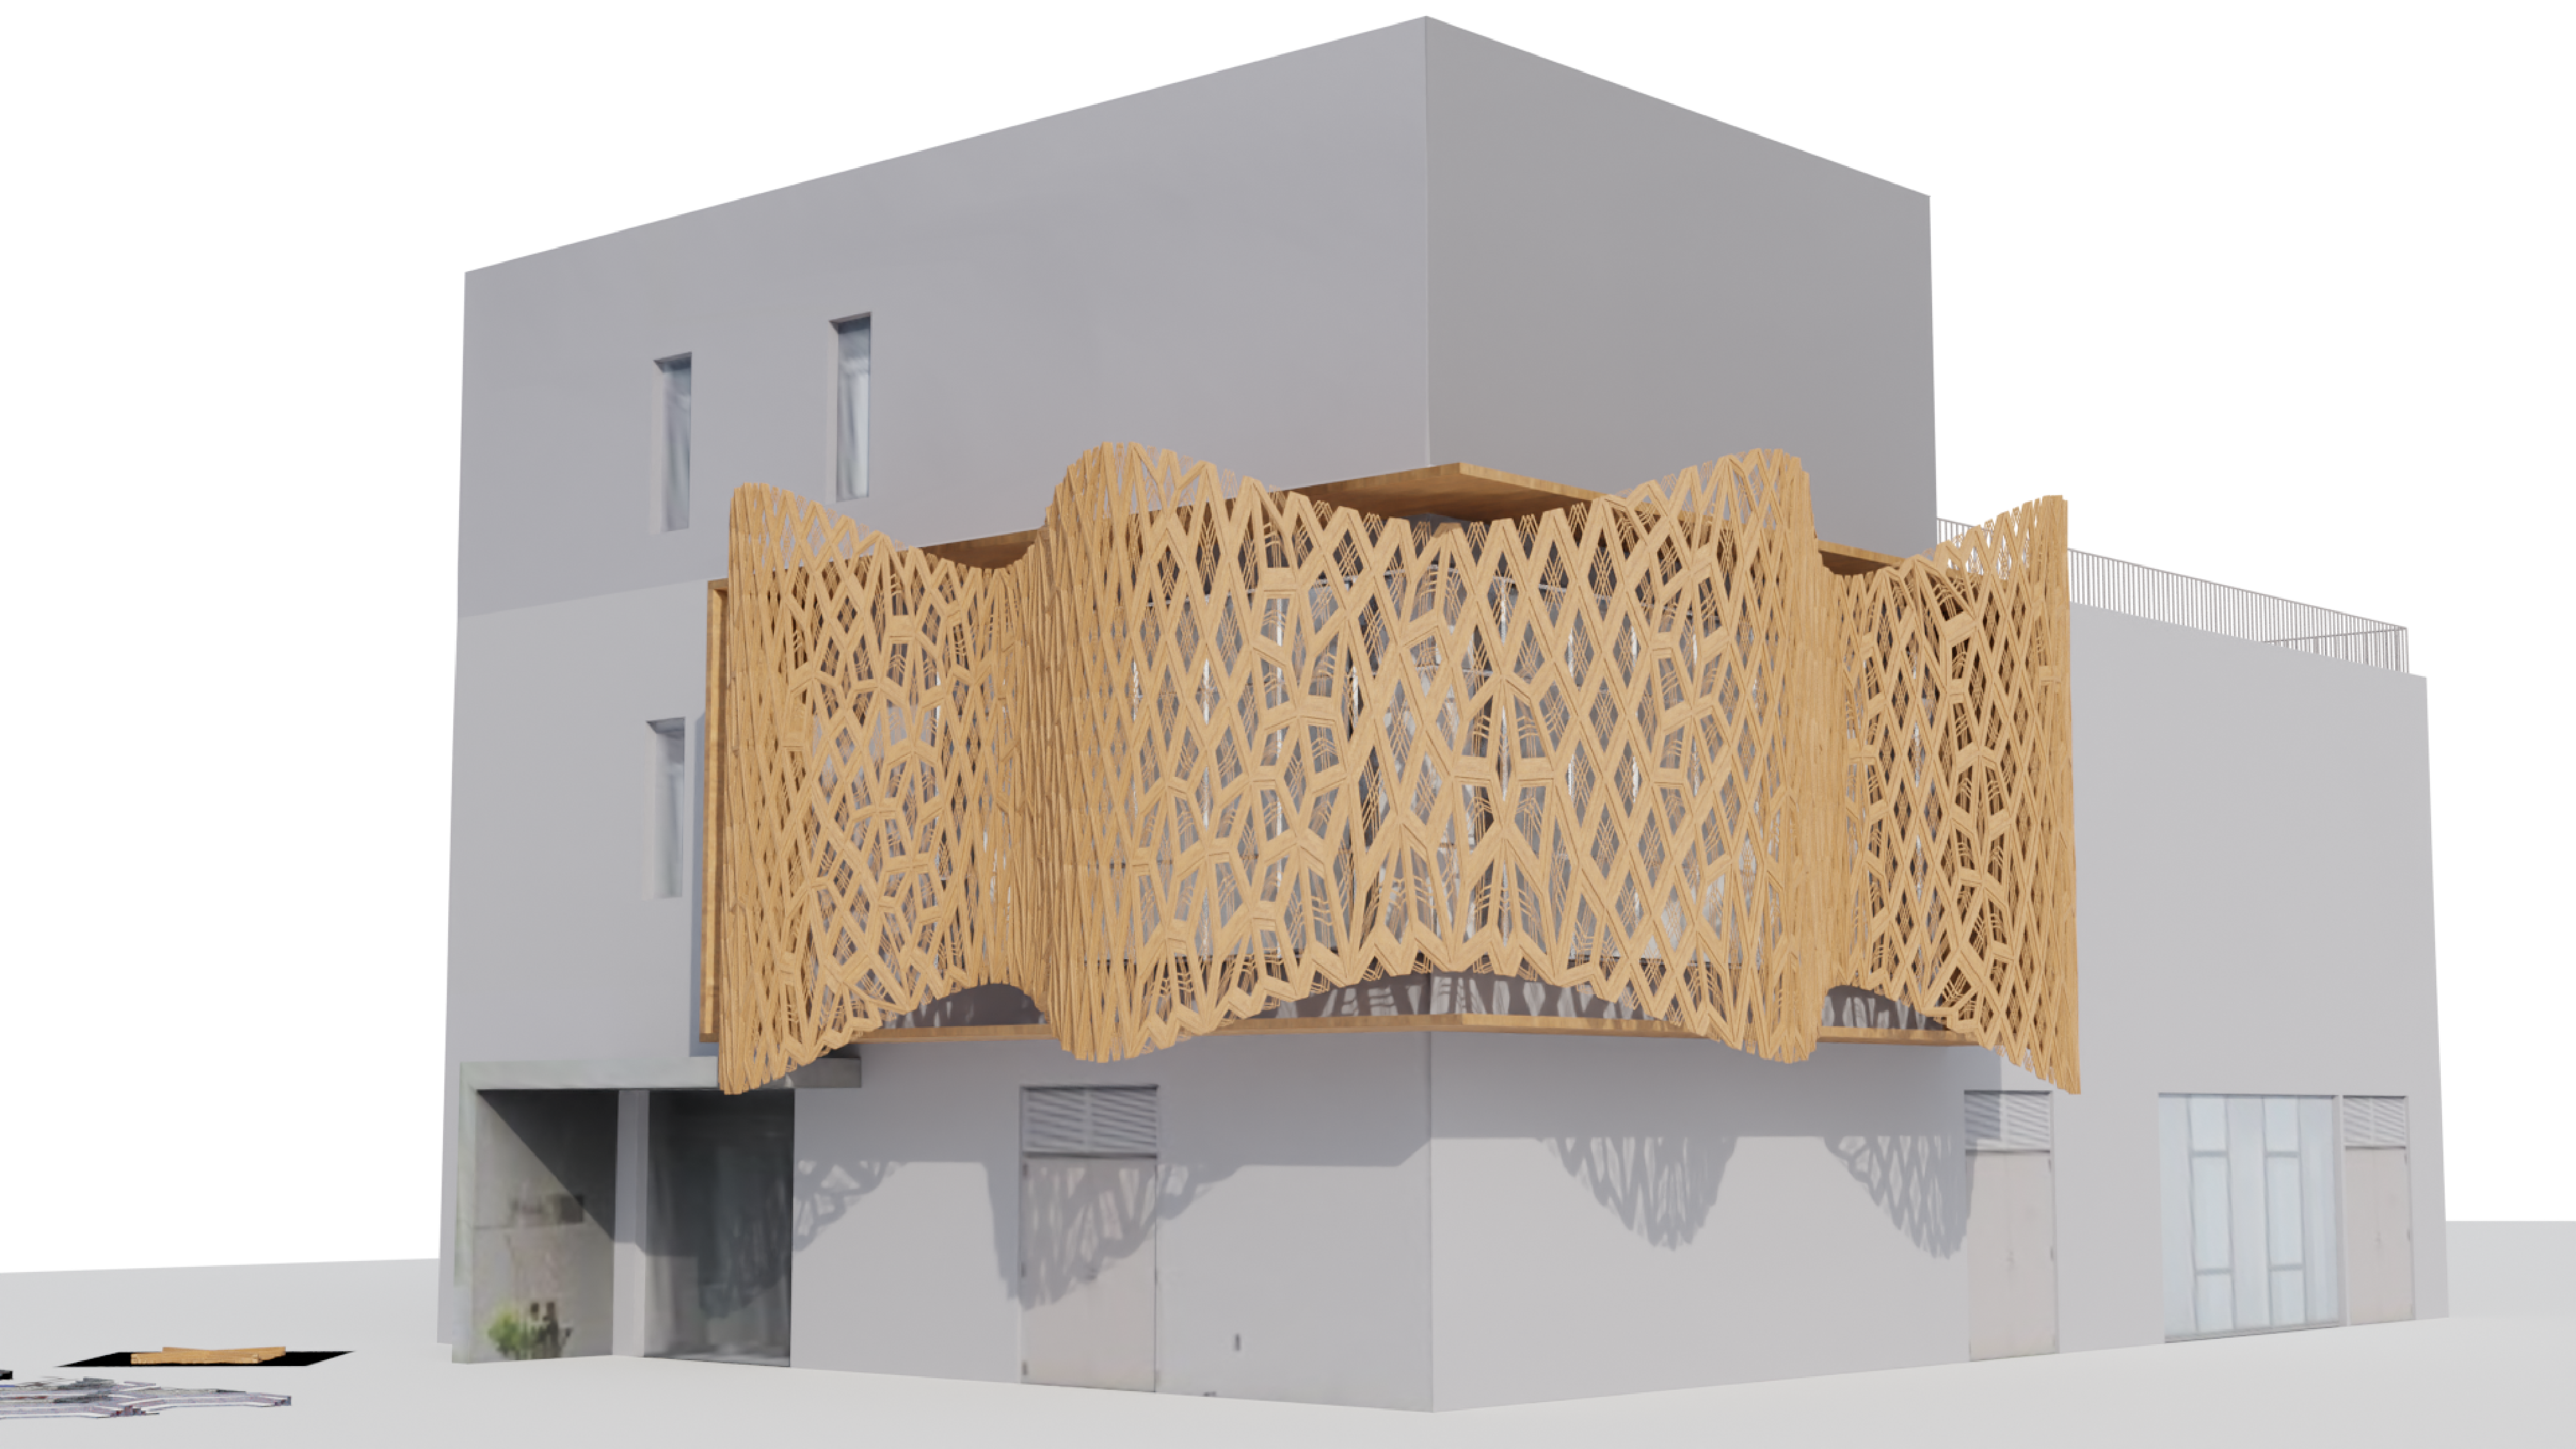
\includegraphics[width=1\linewidth]{Images/Pattern 1/0009}} &
              {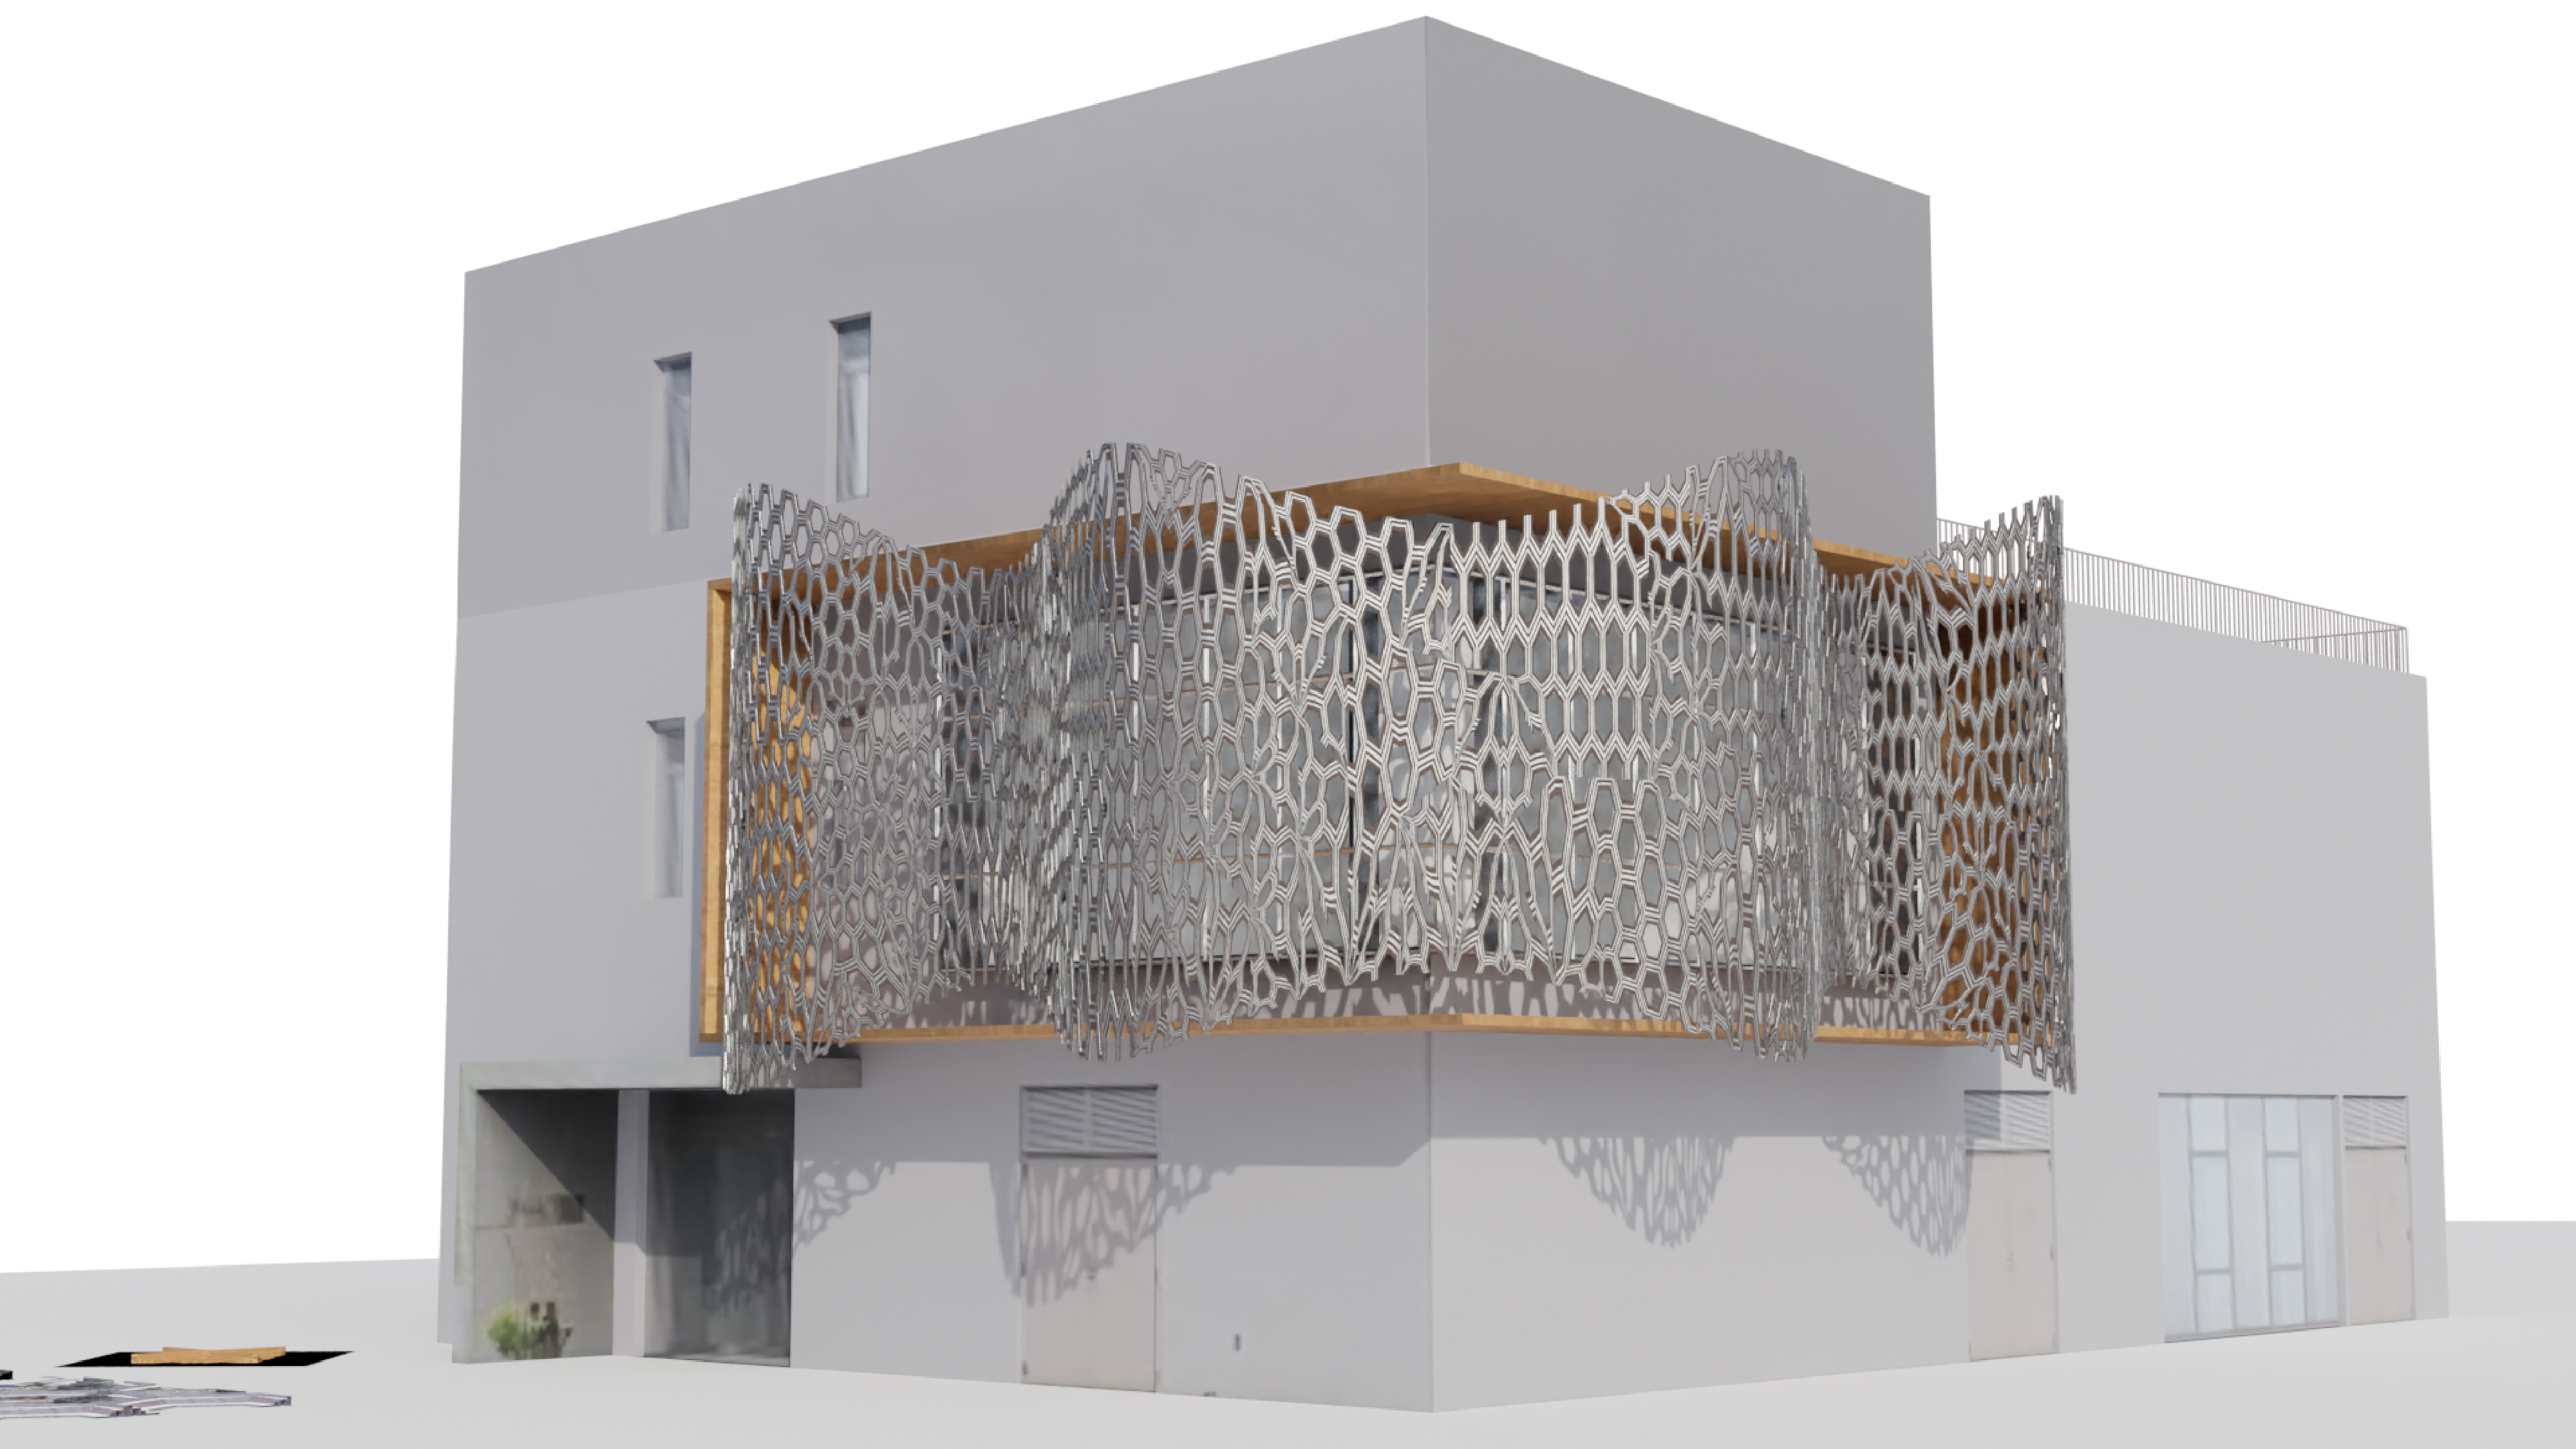
\includegraphics[width=1\linewidth]{Images/Pattern 2/0009}} &
              {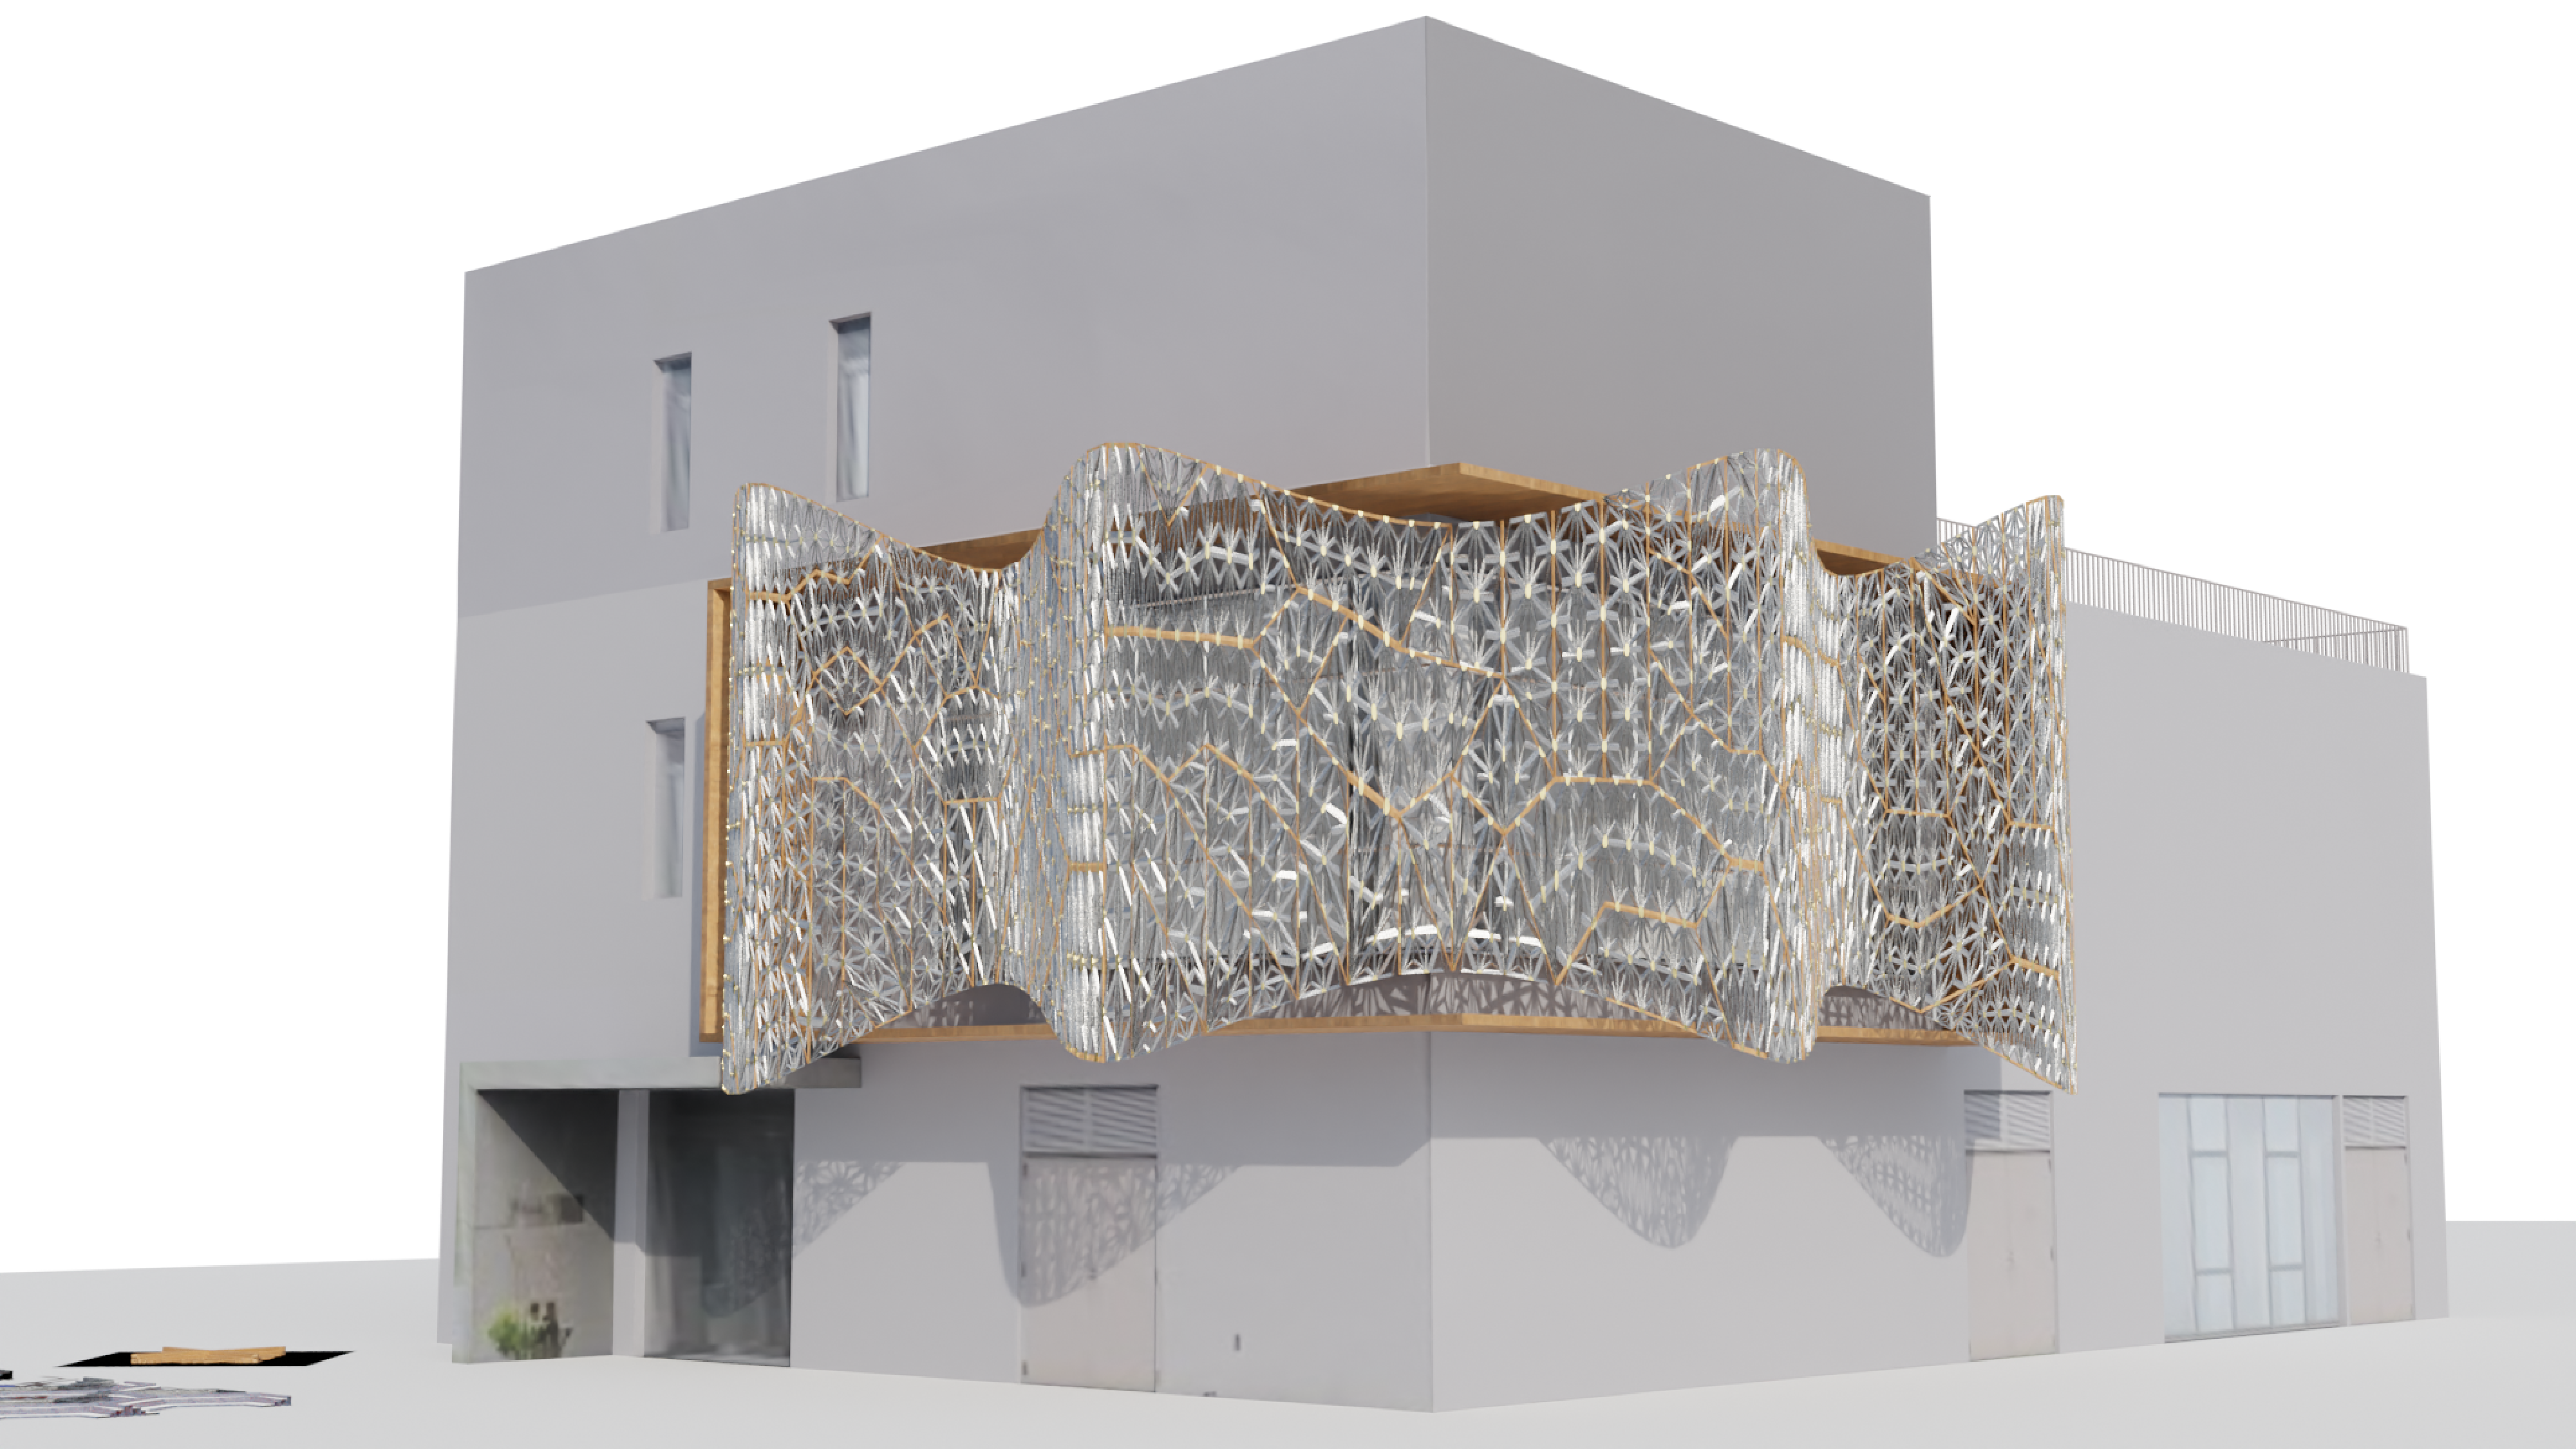
\includegraphics[width=1\linewidth]{Images/Pattern 3/0009}} \\
            \midrule
            \textit{Level 10} &  &  &
            \\
            {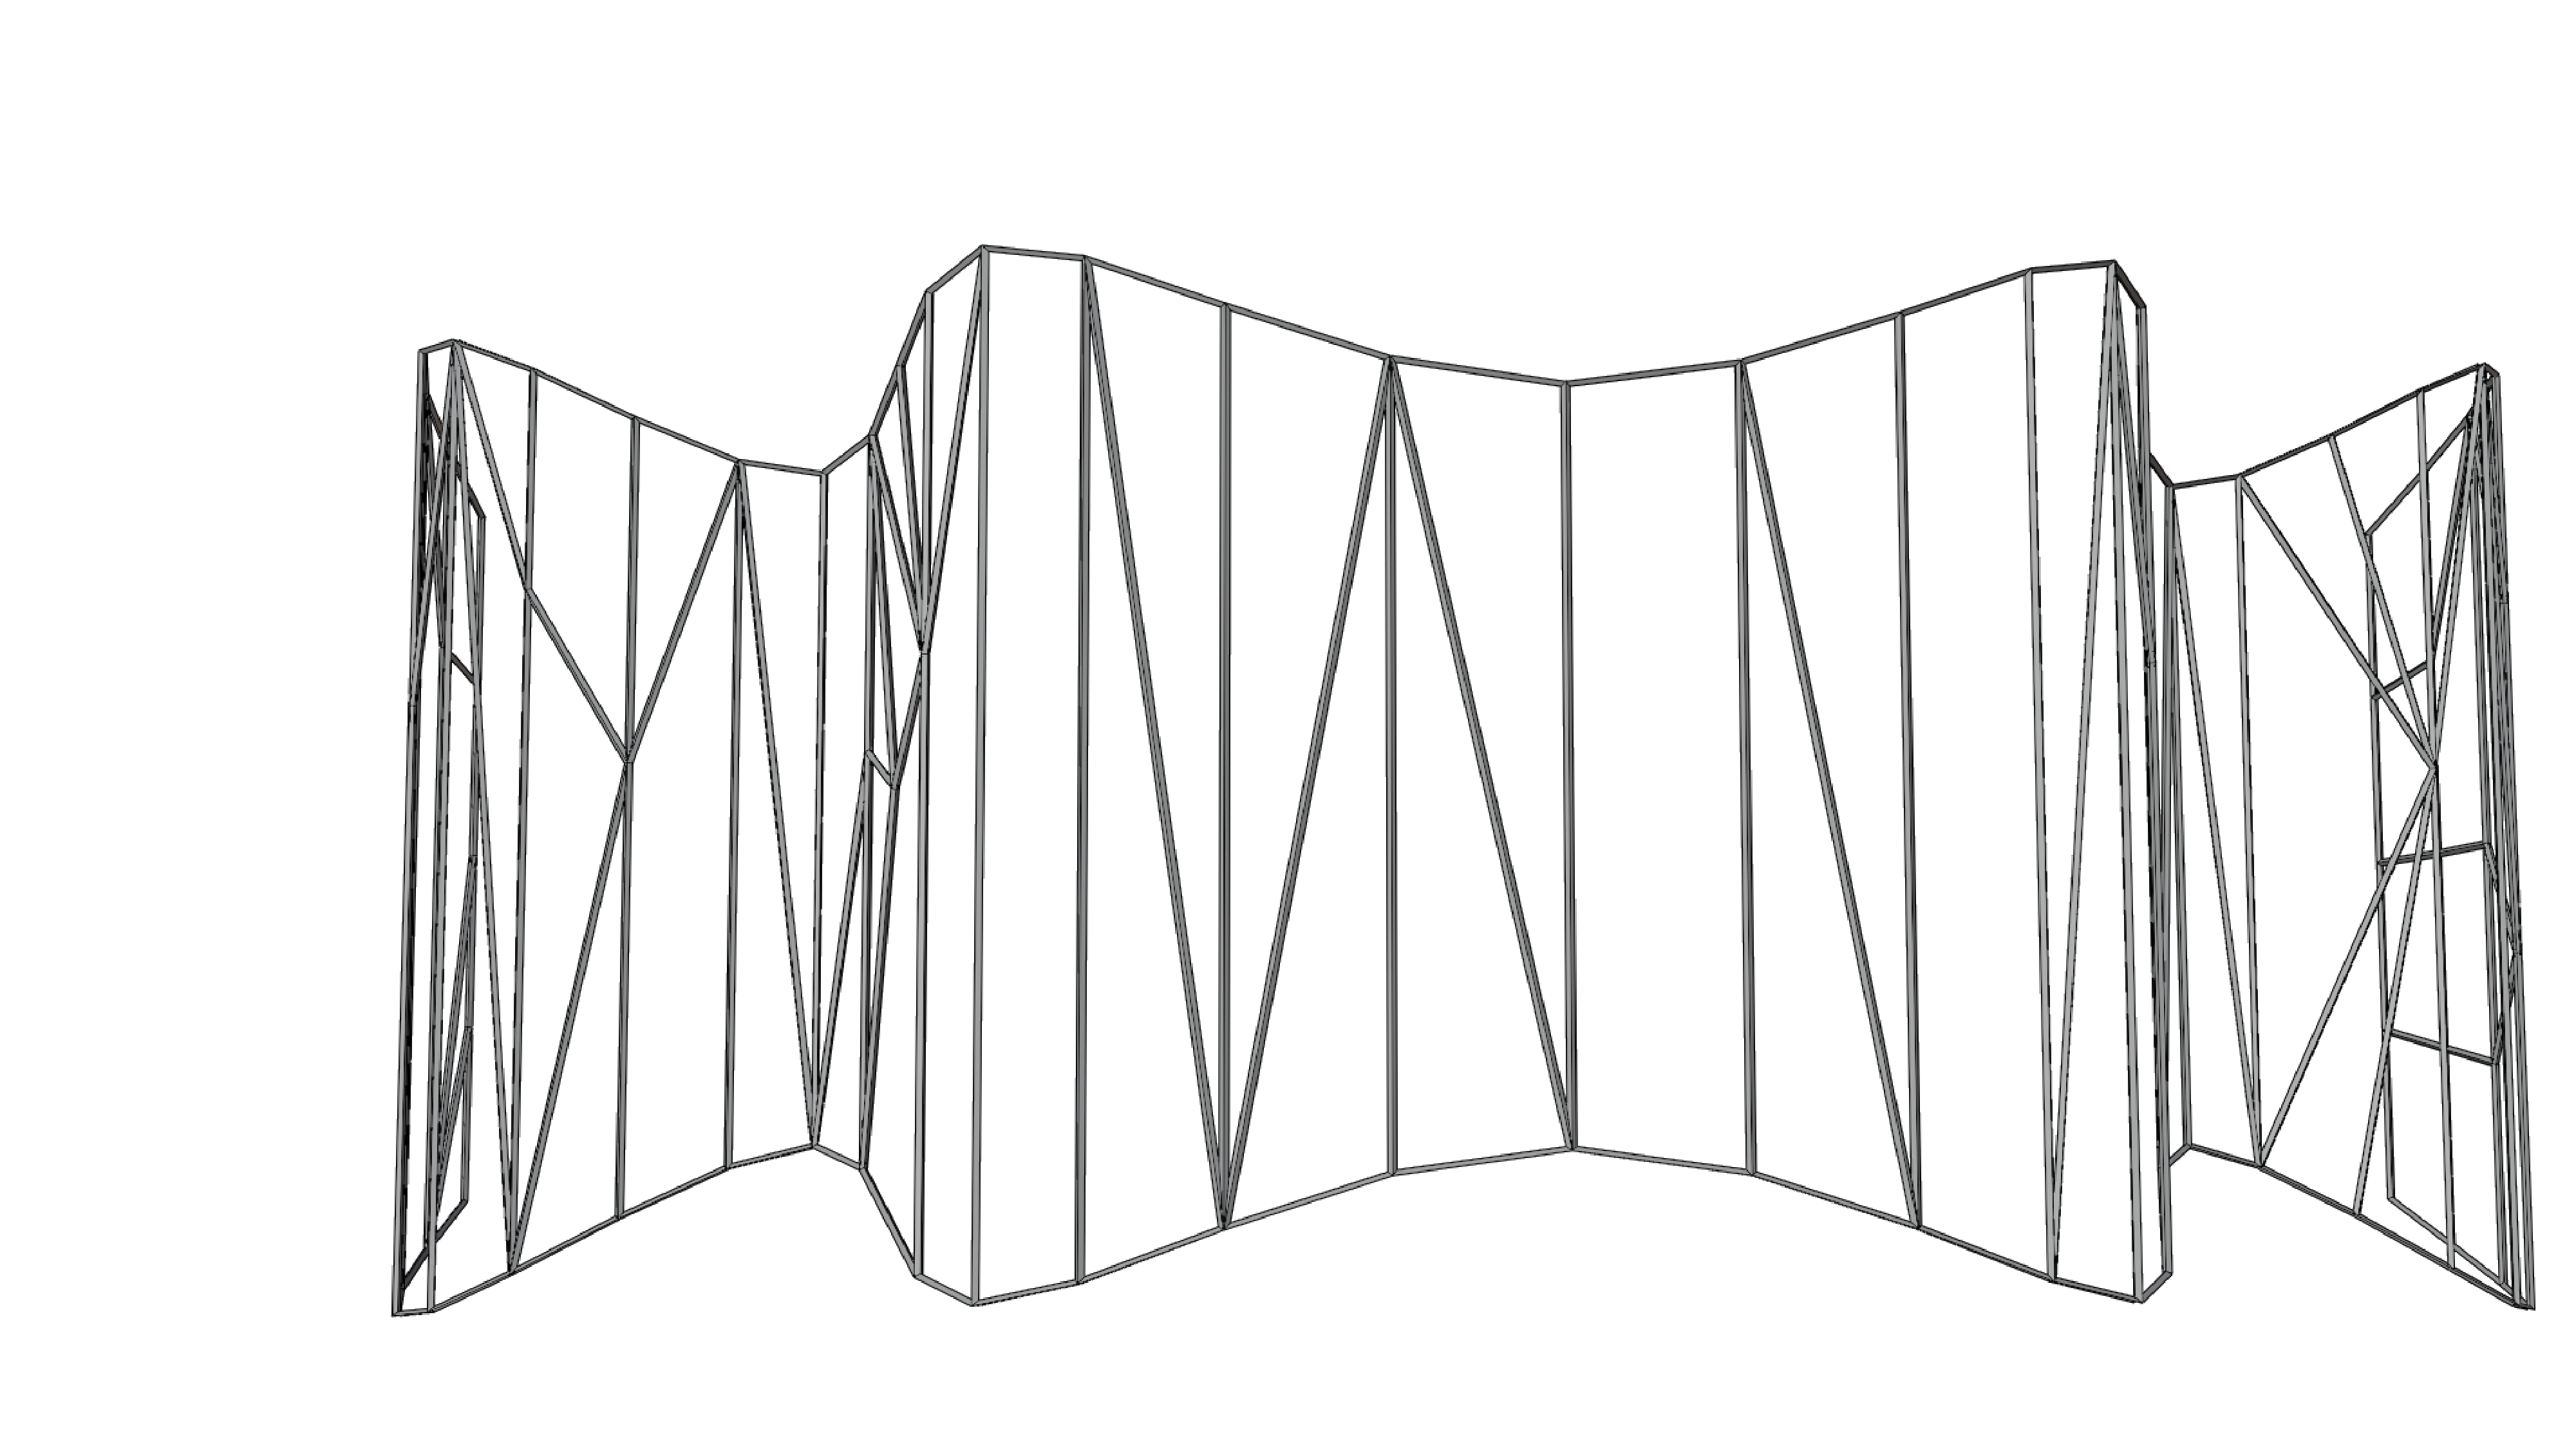
\includegraphics[width=1\linewidth]{Images/Wall 0/0010}} &
              {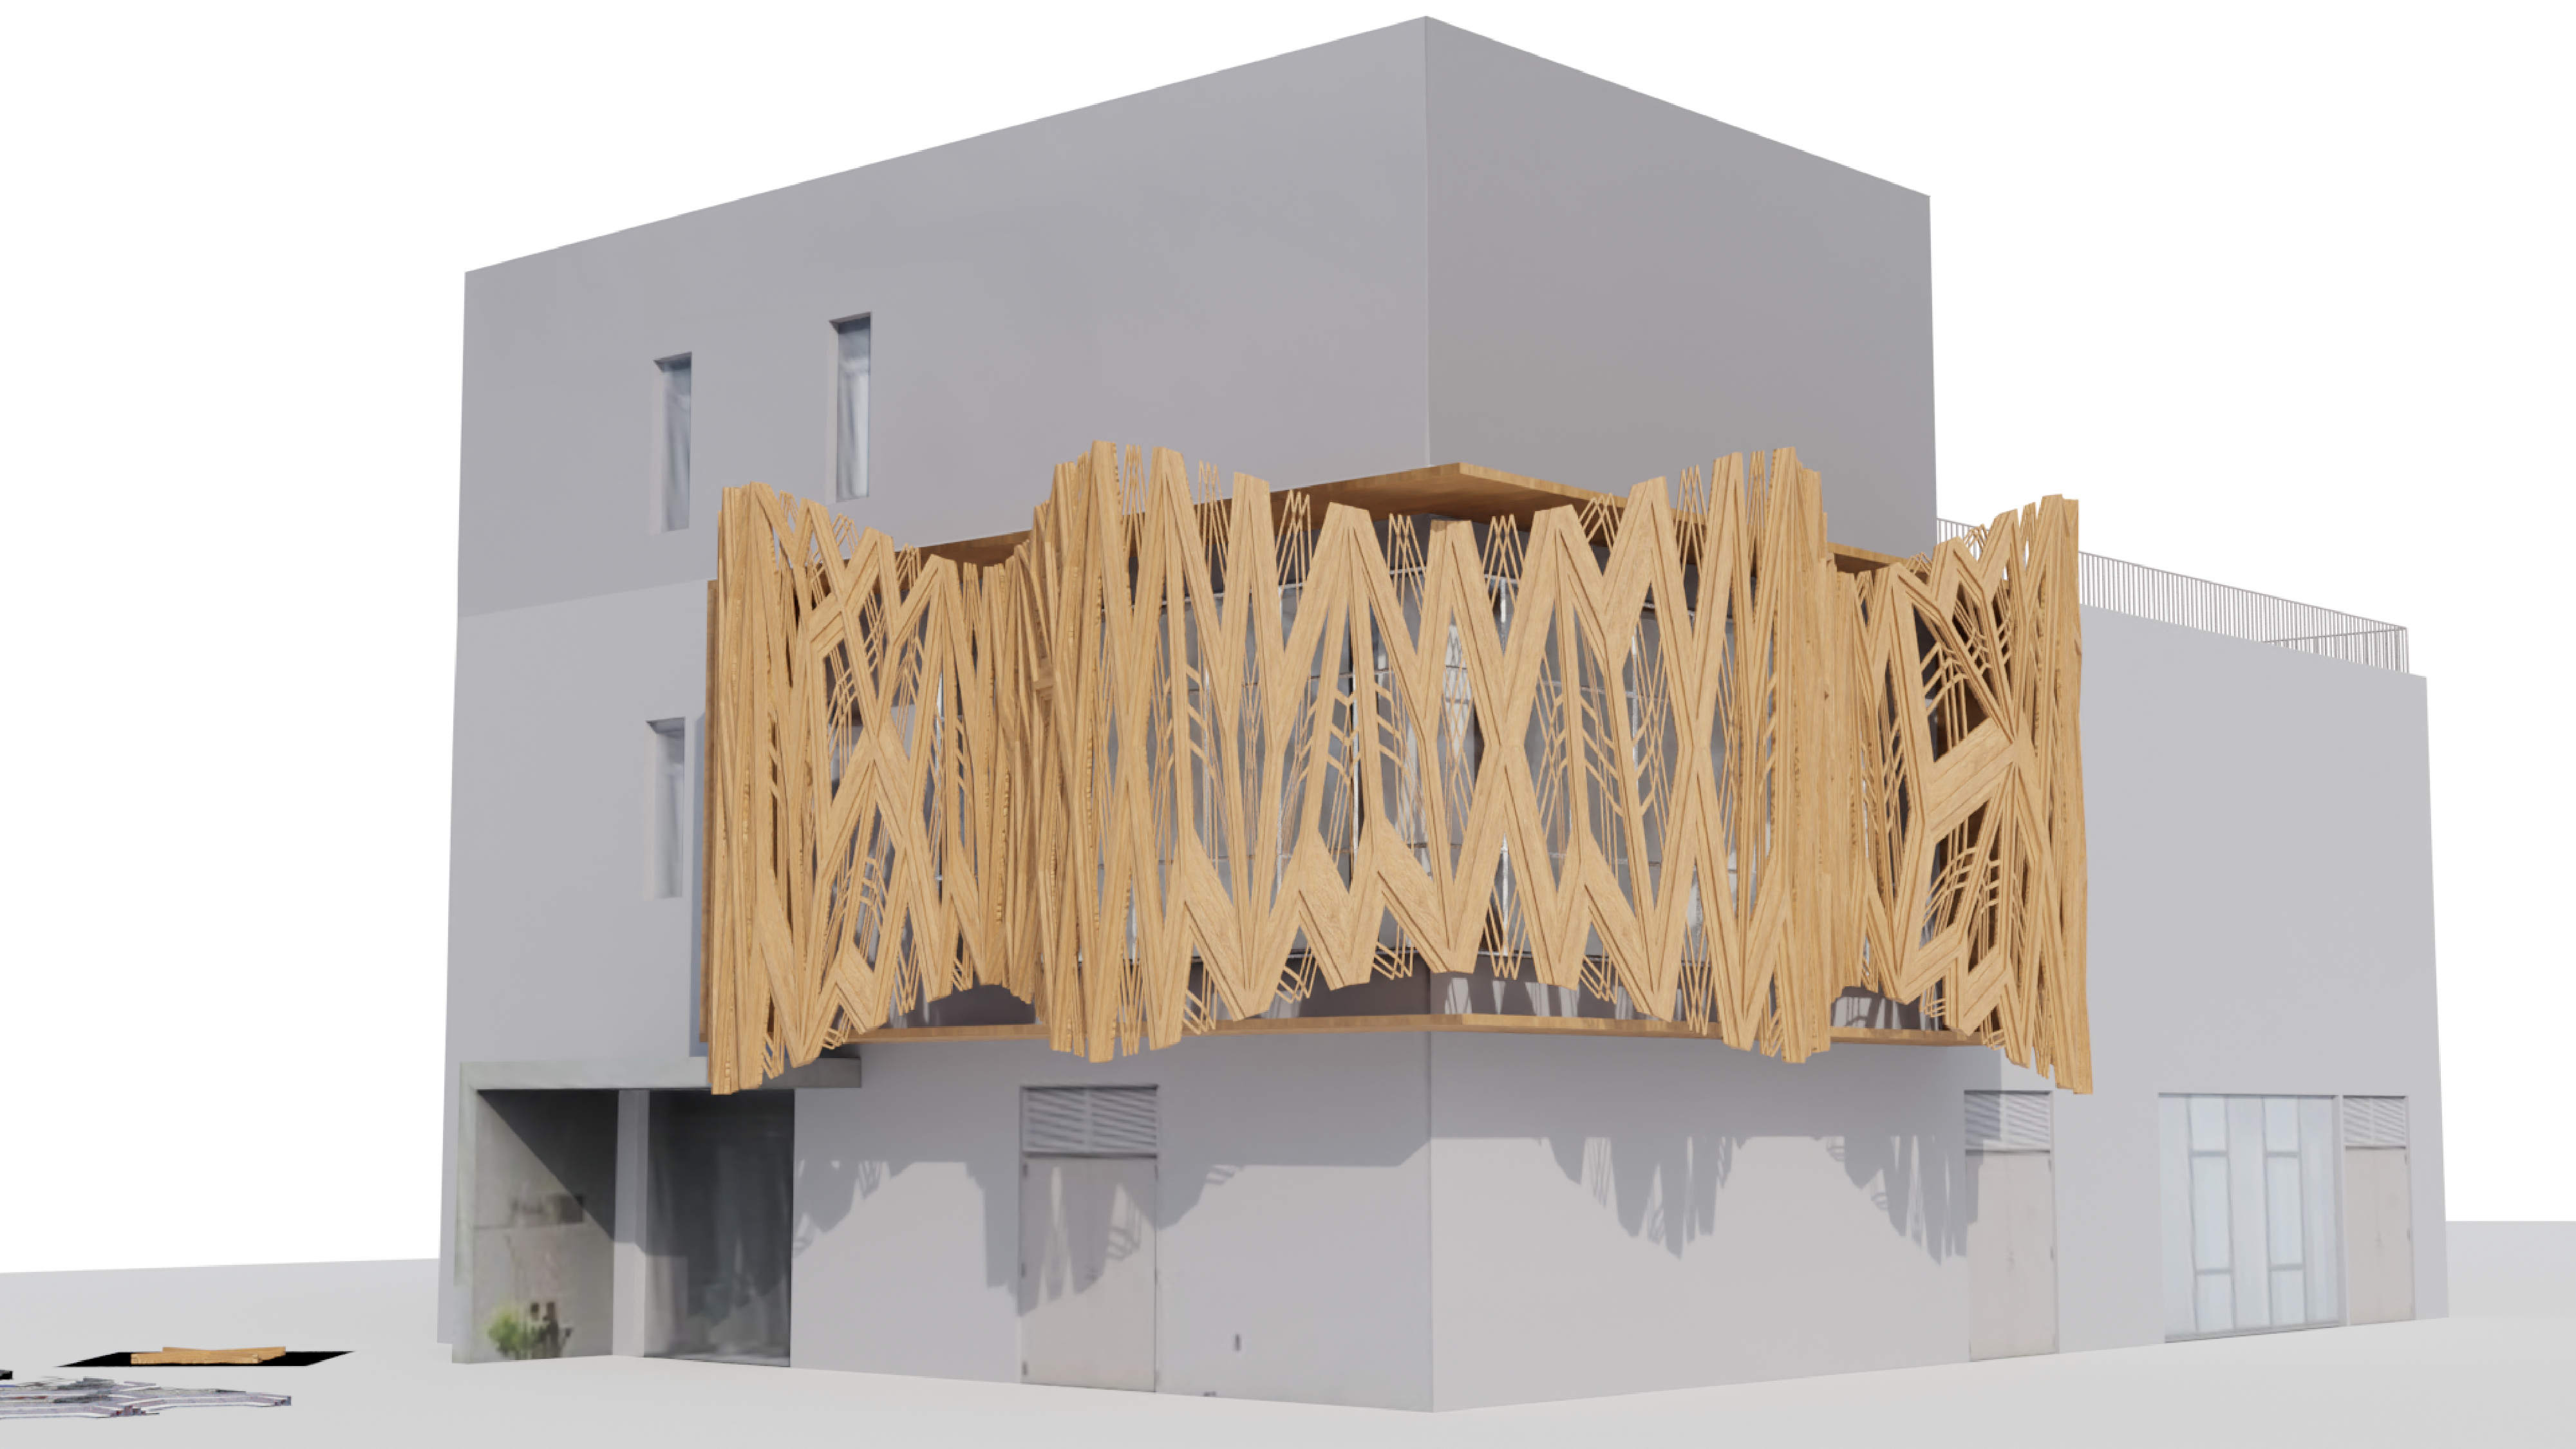
\includegraphics[width=1\linewidth]{Images/Pattern 1/0010}} &
              {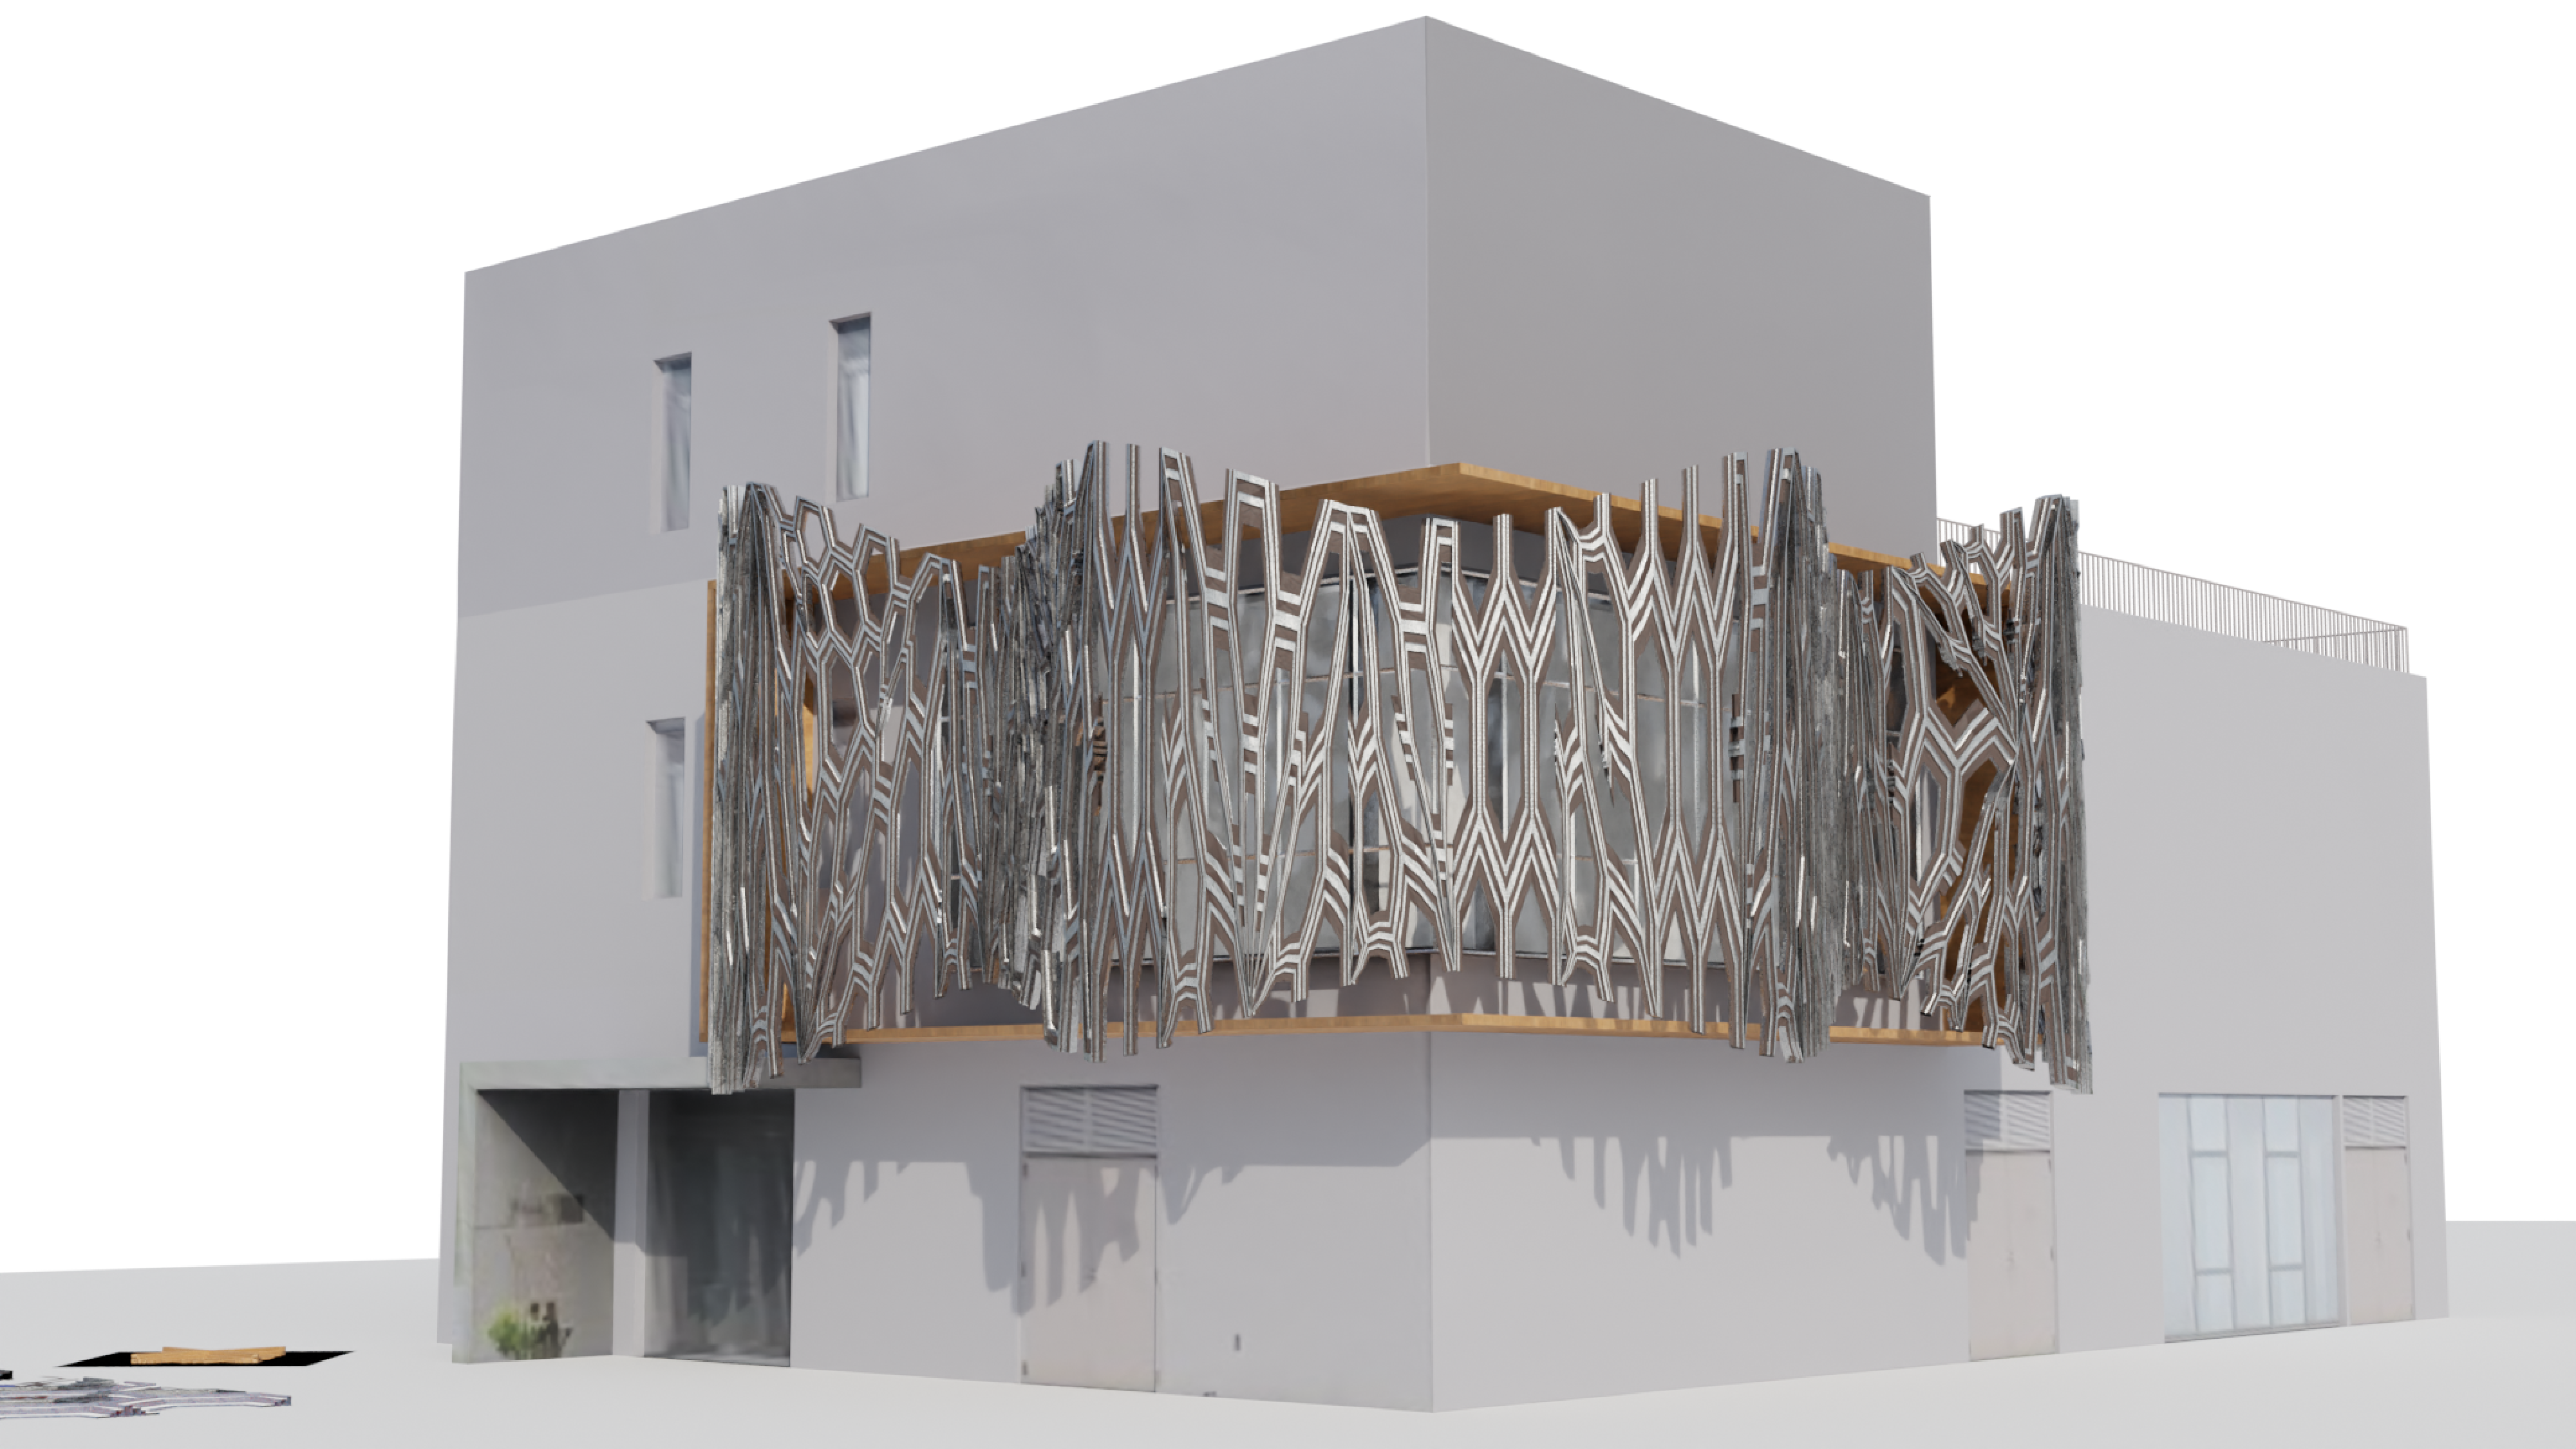
\includegraphics[width=1\linewidth]{Images/Pattern 2/0010}} &
              {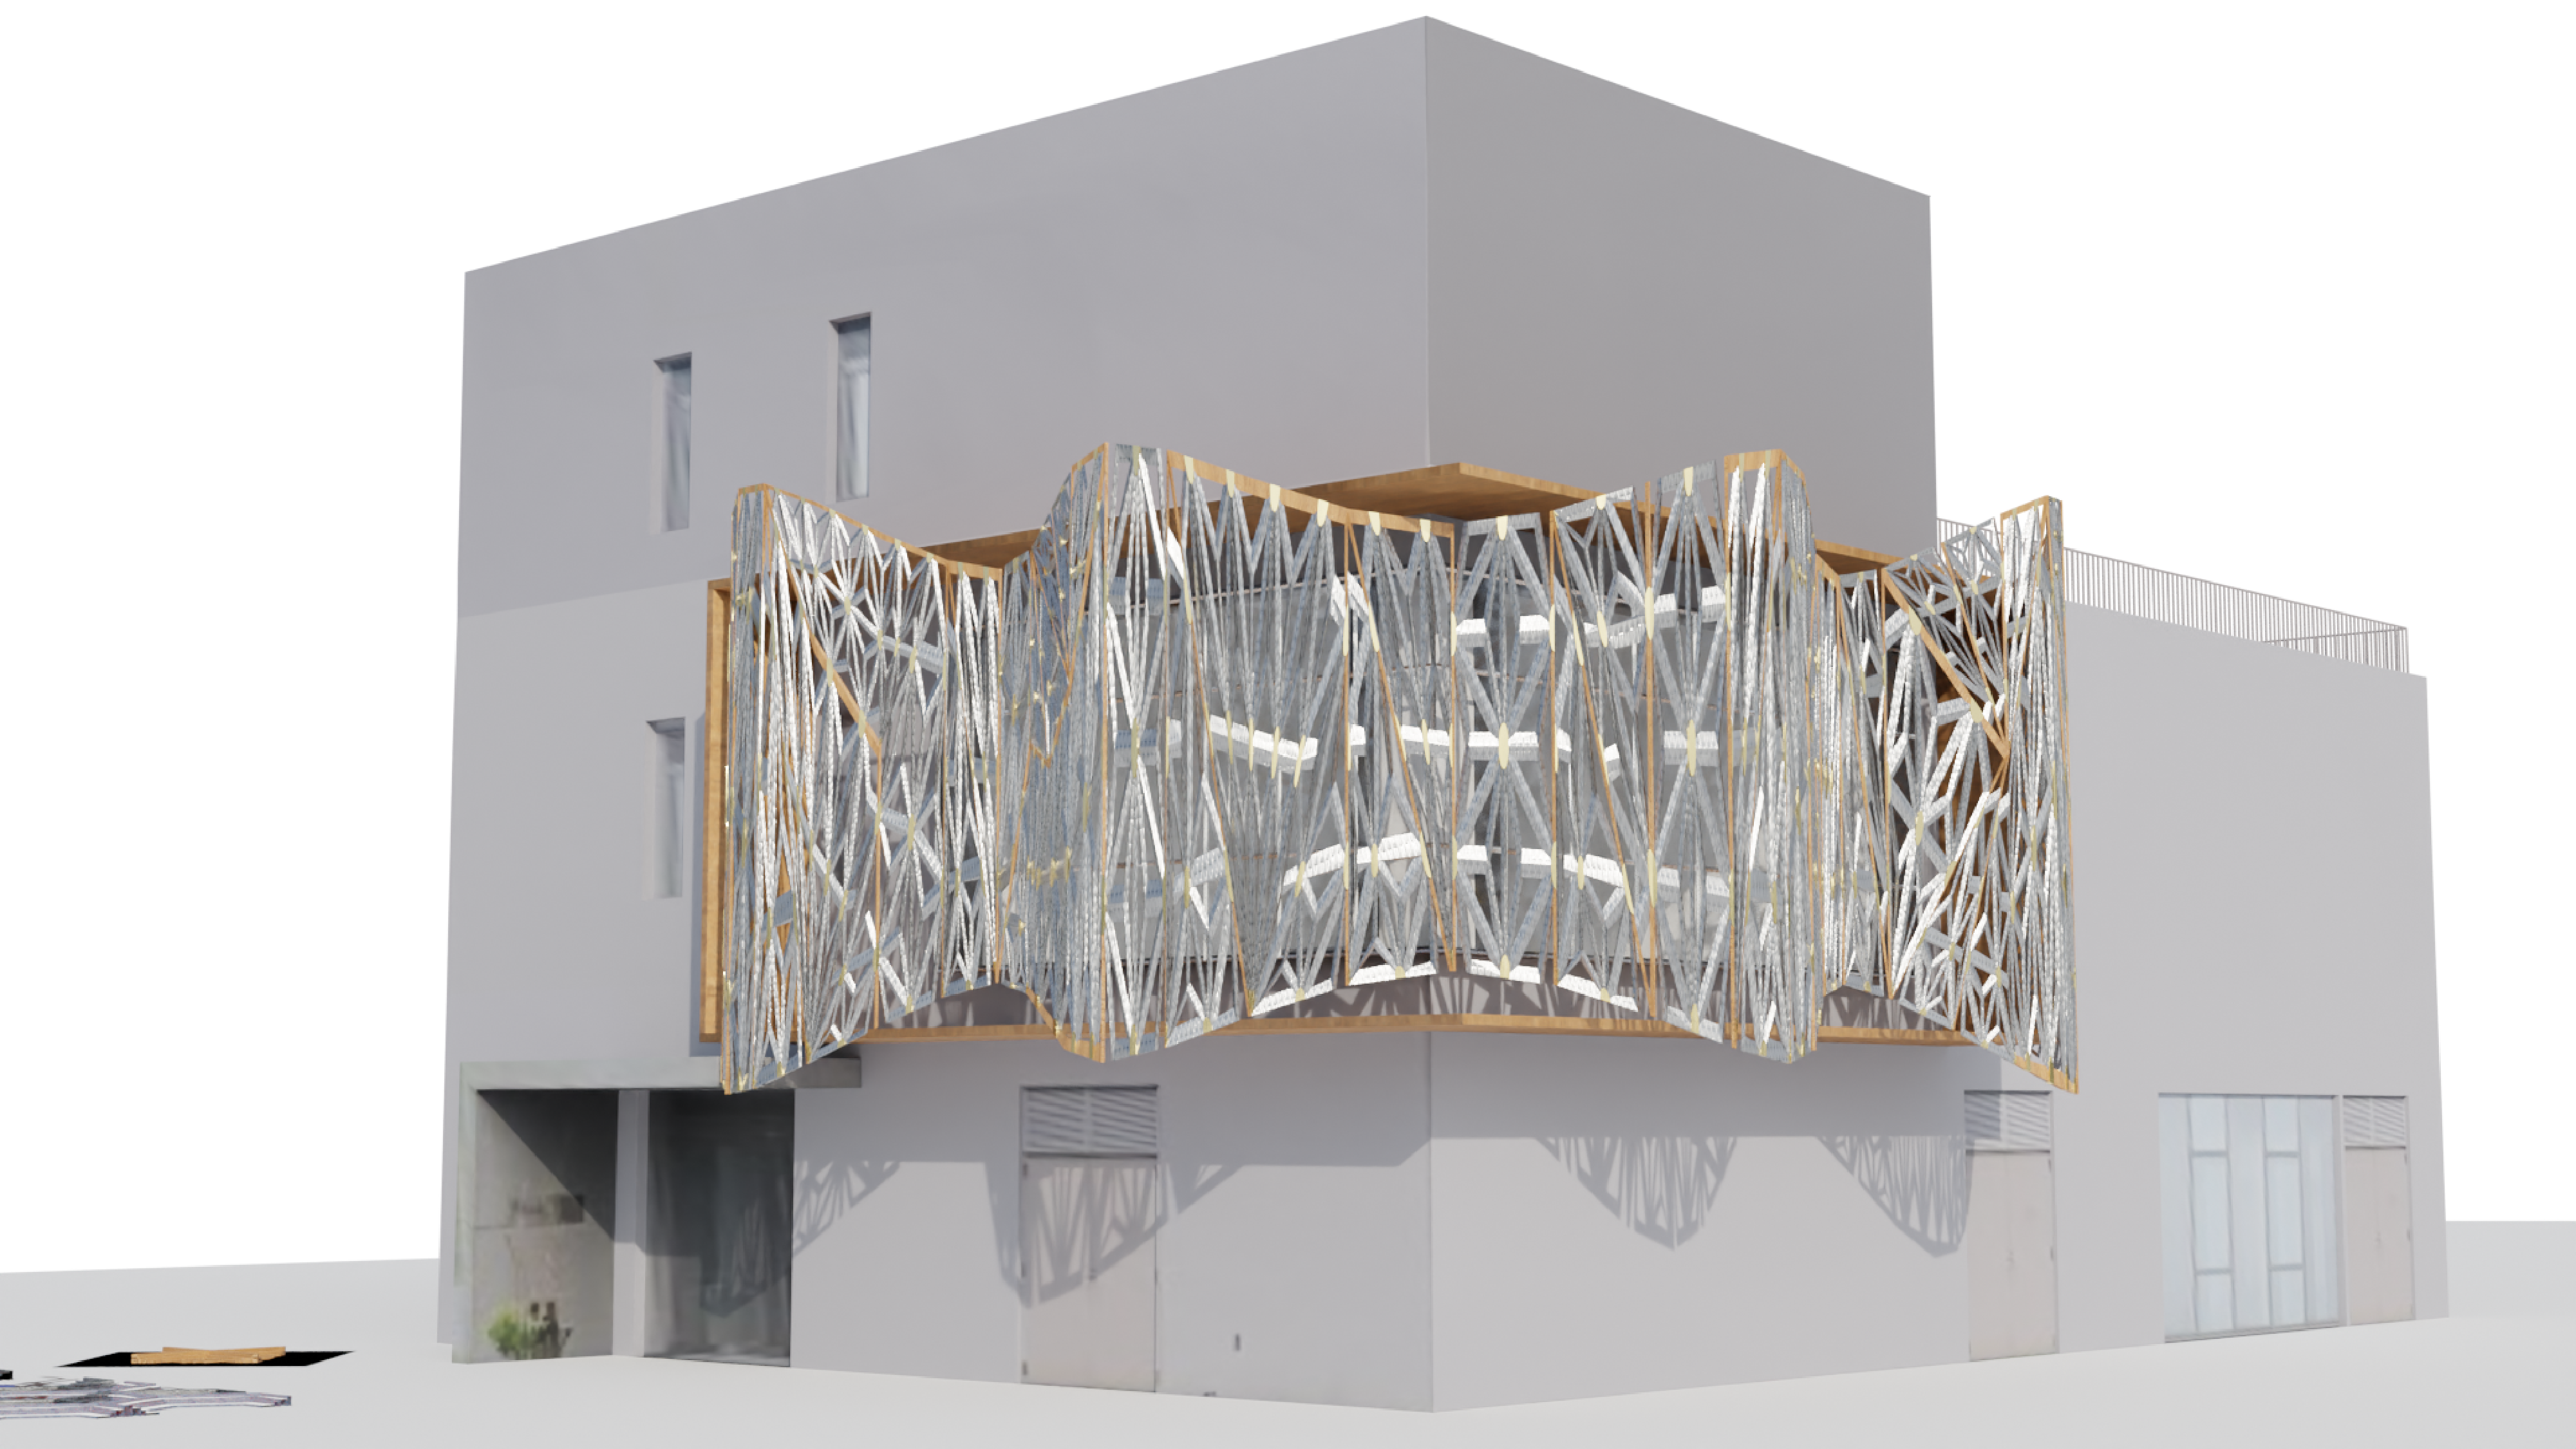
\includegraphics[width=1\linewidth]{Images/Pattern 3/0010}} \\
            \bottomrule
        \end{tabularx}
    \end{table*}



Facade Variations generated for each of the 3 patterns created in Blender and projected during the VR experiment, illustrated in Tables \ref{tab:PatternsVariationsPart1} and \ref{tab:PatternsVariationsPart2}.

    %%Table: Pattern Variations 1 to 5. Part1
    \begin{table*}[htb]
        \centering
        \small
        \caption{Patterns variations for the First five levels of complexity}
        \label{tab:PatternsVariationsPart1}
        \begin{tabularx}
        {\textwidth}{p{3cm} >{\centering\arraybackslash}X >{\centering\arraybackslash}X >{\centering\arraybackslash}X }
            \toprule
            \textit{Description} &
              \textit{Pattern 1} &
              \textit{Pattern 2} &
              \textit{Pattern 3} \\
            \midrule
            \text{Pattern Name} & Hishi Pattern & Tortoise shells & Asanoha Pattern\\

            \midrule
            \textit{Base Module} &  &  &
            \\
            {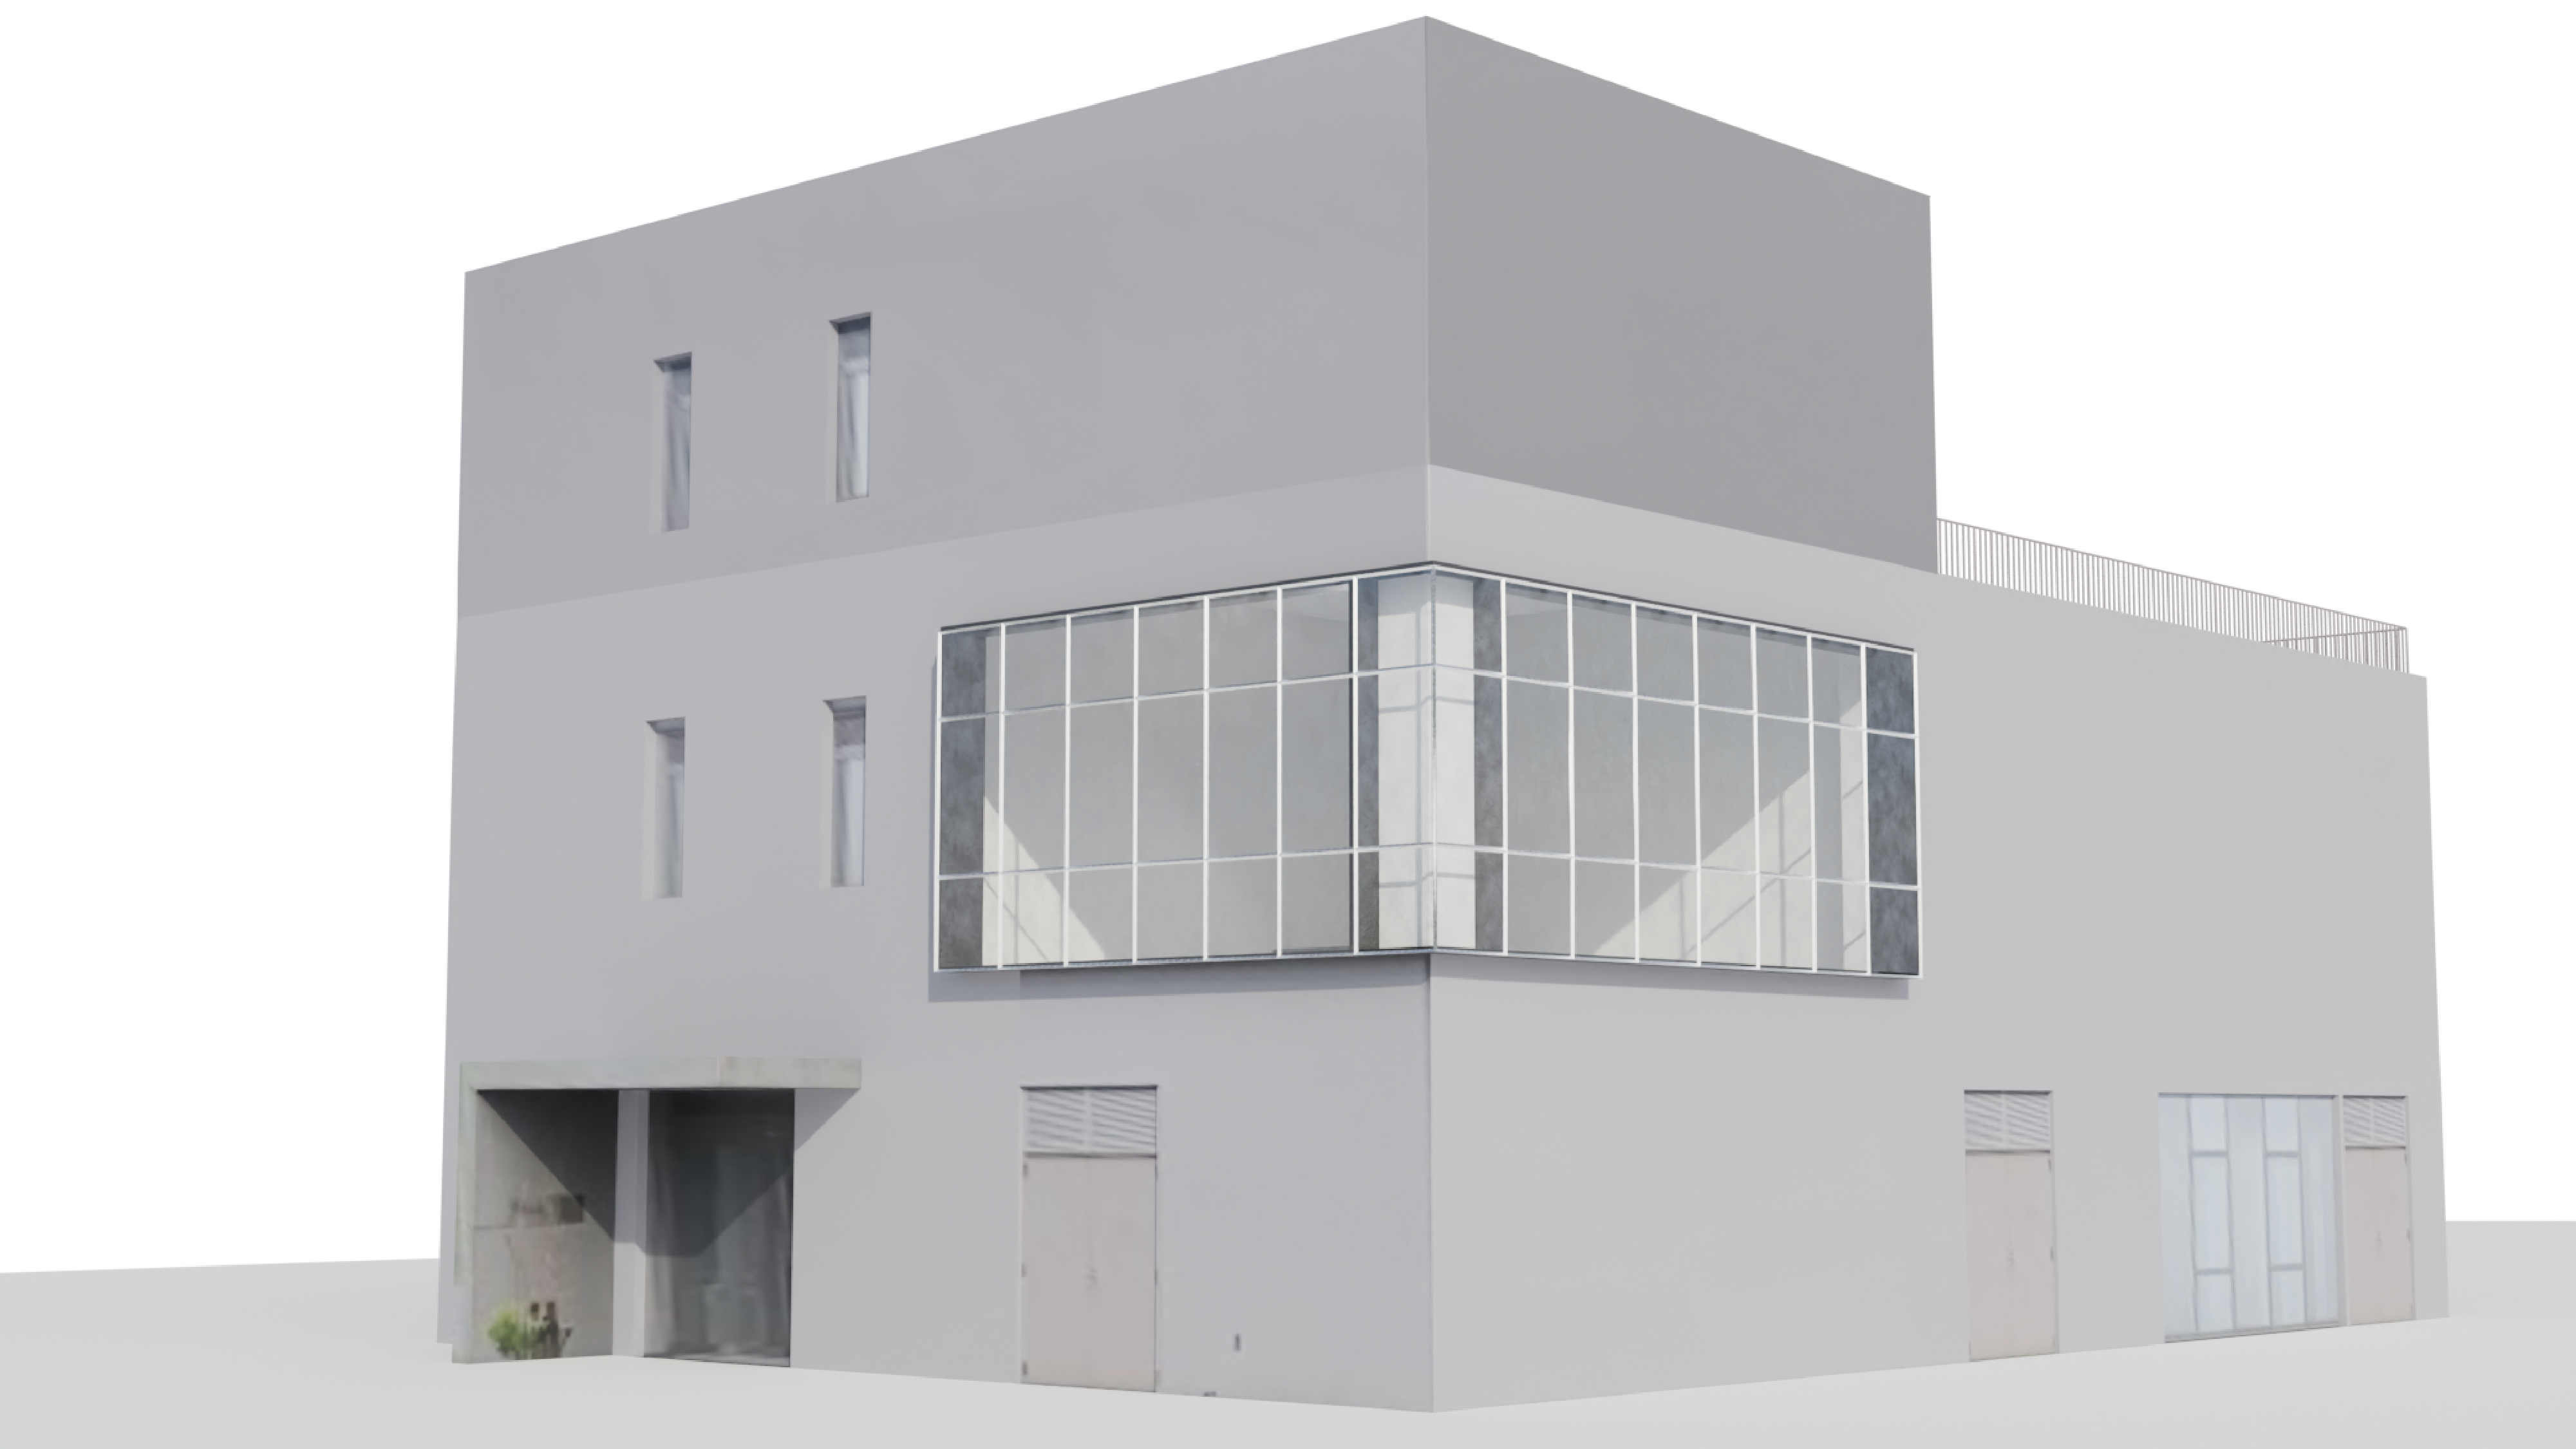
\includegraphics[width=1\linewidth]{Images/Base Module/Building}} &
              {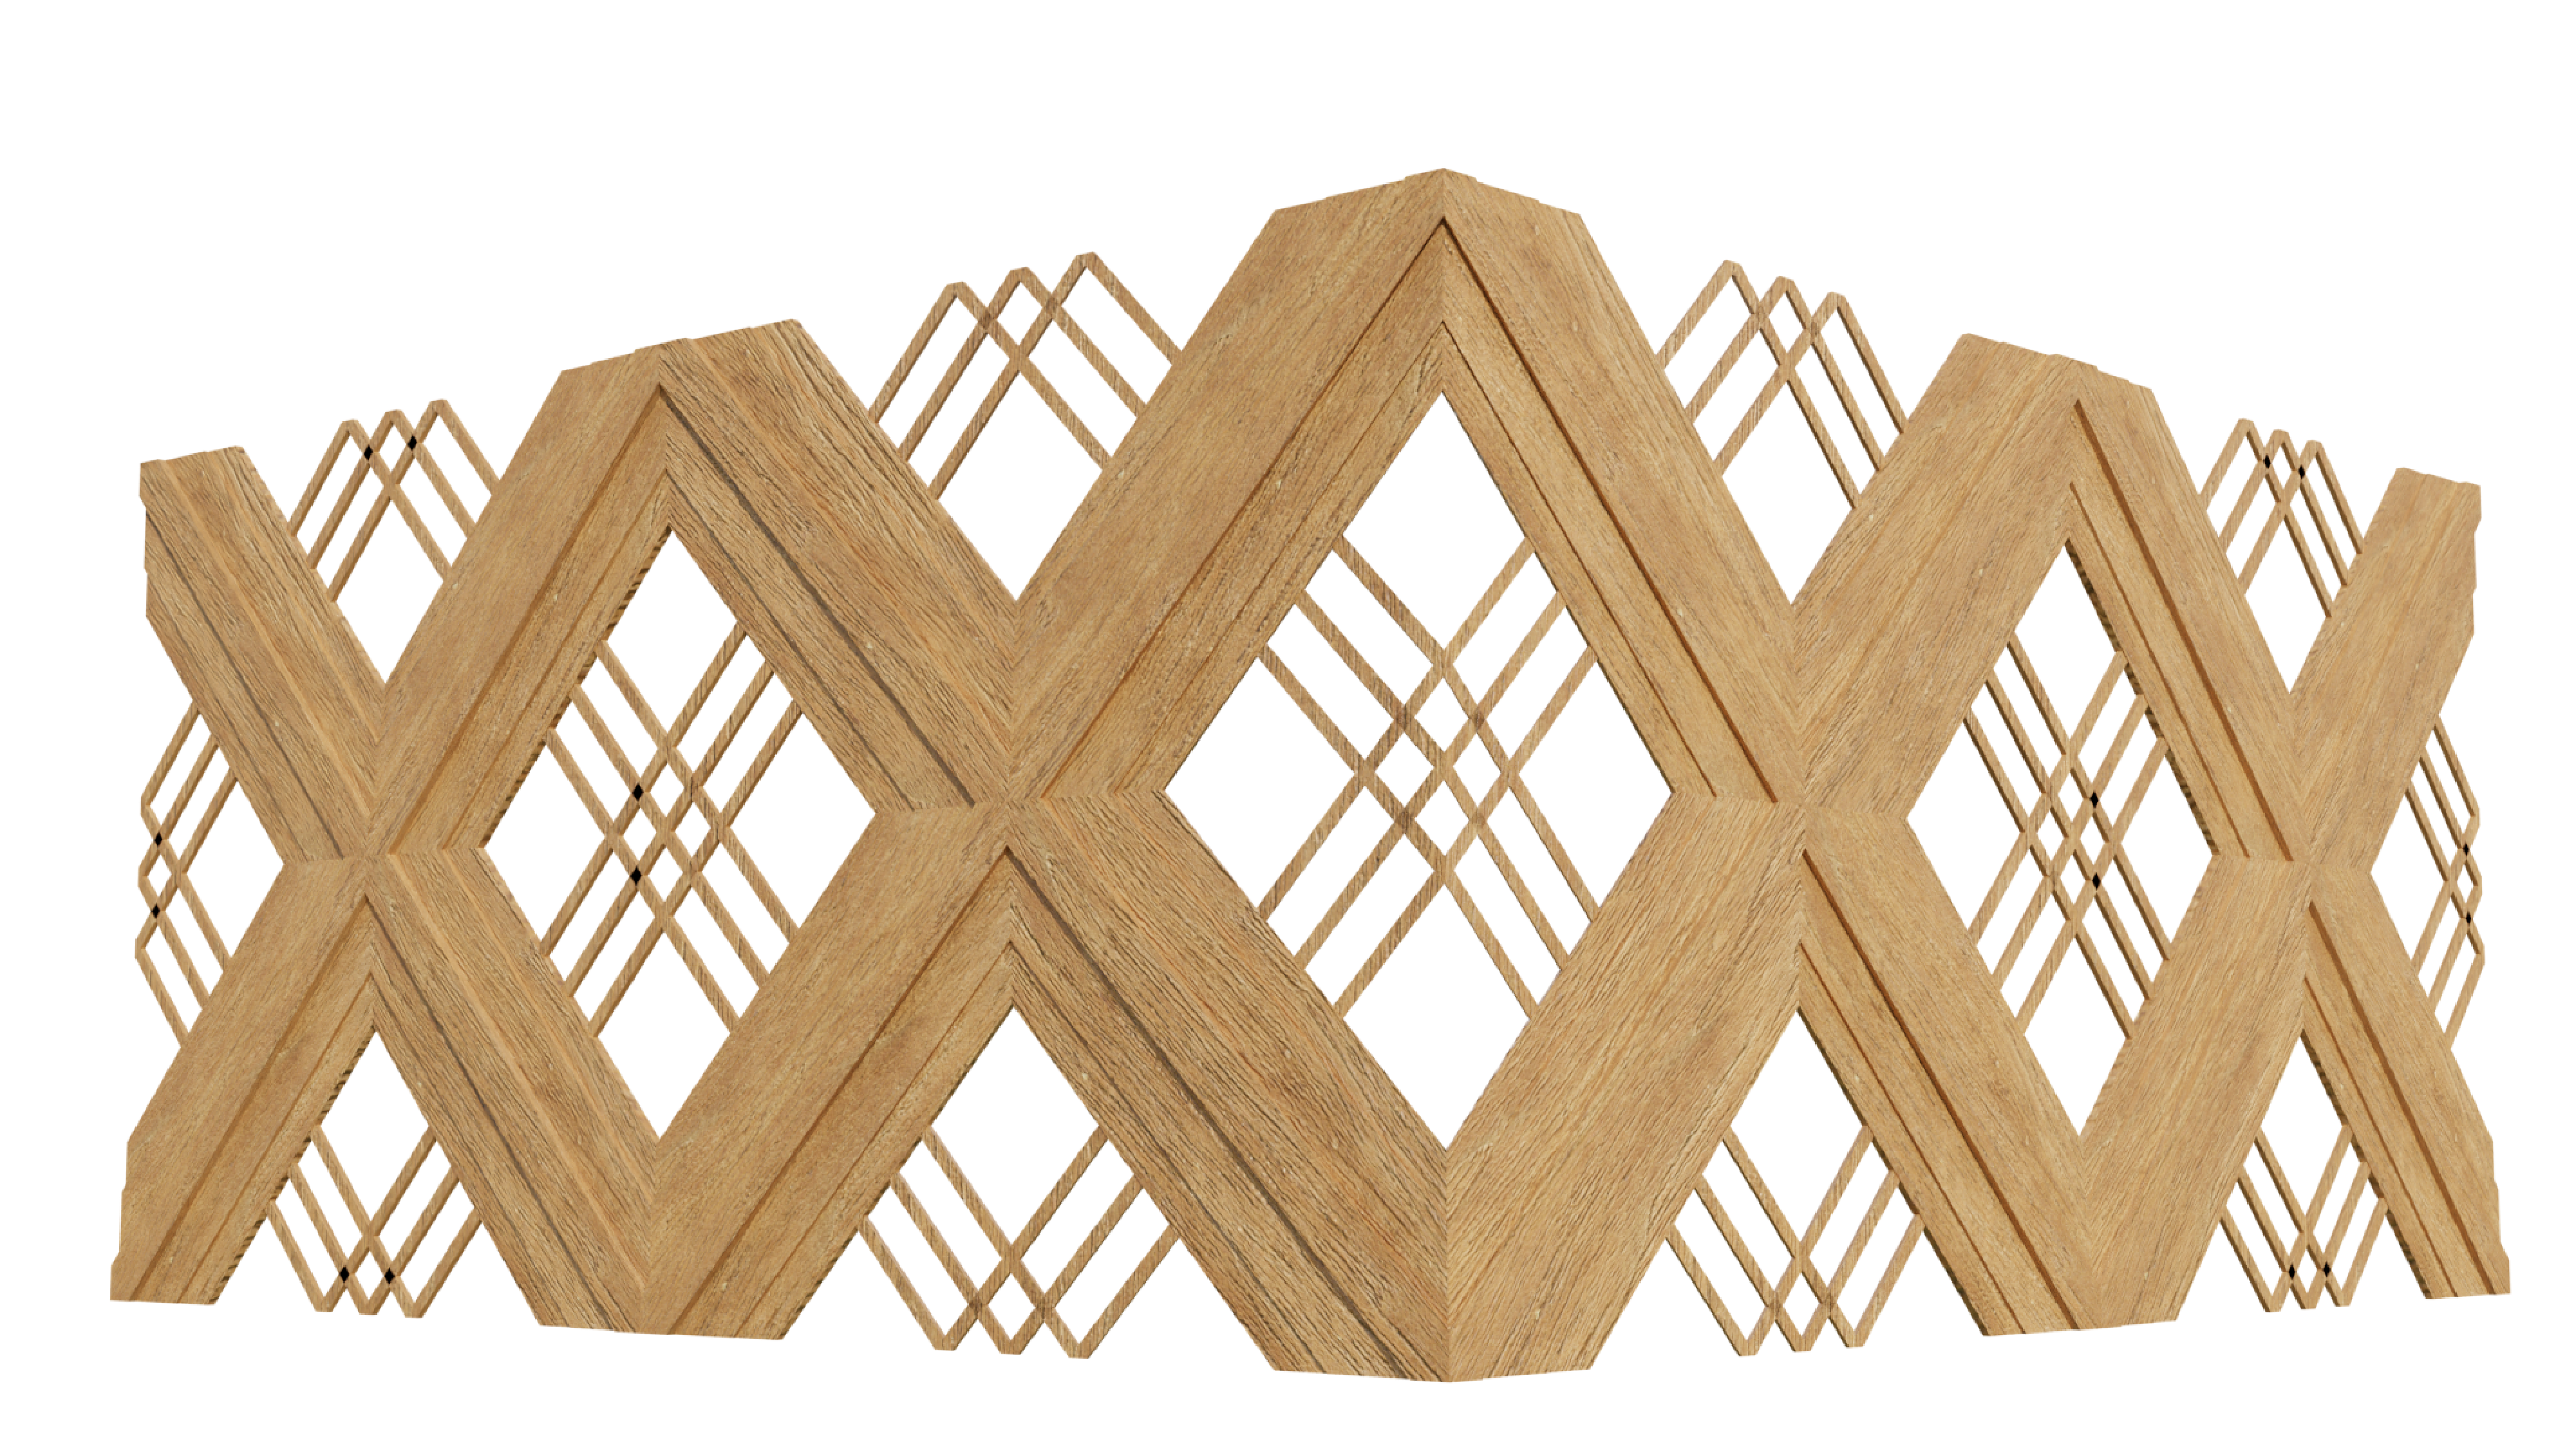
\includegraphics[width=1\linewidth]{Images/Base Module/Pattern1}} &
              {\includegraphics[width=1\linewidth]{Images/Base Module/Pattern2}} &
              {\includegraphics[width=1\linewidth]{Images/Base Module/Pattern3}} \\
            \midrule

            \textit{Mesh complexity Level} &
              \textit{Pattern 1} &
              \textit{Pattern 2} &
              \textit{Pattern 3}\\

            \midrule
            \textit{Level 1} &  &  &
            \\
            {\includegraphics[width=1\linewidth]{Images/Wall 0/0001}} &
                {\includegraphics[width=1\linewidth]{Images/Pattern 1/0001}} &
              {\includegraphics[width=1\linewidth]{Images/Pattern 2/0001}} &
              {\includegraphics[width=1\linewidth]{Images/Pattern 3/0001}} \\
            \midrule
            \textit{Level 2} &  &  &
            \\
            {\includegraphics[width=1\linewidth]{Images/Wall 0/0002}} &
              {\includegraphics[width=1\linewidth]{Images/Pattern 1/0002}} &
              {\includegraphics[width=1\linewidth]{Images/Pattern 2/0002}} &
              {\includegraphics[width=1\linewidth]{Images/Pattern 3/0002}} \\
            \midrule
            \textit{Level 3} &  &  &
            \\
            {\includegraphics[width=1\linewidth]{Images/Wall 0/0003}} &
              {\includegraphics[width=1\linewidth]{Images/Pattern 1/0003}} &
              {\includegraphics[width=1\linewidth]{Images/Pattern 2/0003}} &
              {\includegraphics[width=1\linewidth]{Images/Pattern 3/0003}} \\
            \midrule
            \textit{Level 4} &  &  &
            \\
            {\includegraphics[width=1\linewidth]{Images/Wall 0/0004}} &
              {\includegraphics[width=1\linewidth]{Images/Pattern 1/0004}} &
              {\includegraphics[width=1\linewidth]{Images/Pattern 2/0004}} &
              {\includegraphics[width=1\linewidth]{Images/Pattern 3/0004}} \\
            \midrule
            \textit{Level 5} &  &  &
            \\
            {\includegraphics[width=1\linewidth]{Images/Wall 0/0005}} &
              {\includegraphics[width=1\linewidth]{Images/Pattern 1/0005}} &
              {\includegraphics[width=1\linewidth]{Images/Pattern 2/0005}} &
              {\includegraphics[width=1\linewidth]{Images/Pattern 3/0005}} \\
            \bottomrule
        \end{tabularx}
    \end{table*}

    %%Table: Pattern Variations 6 to 10. Part2
    \begin{table*}[htb]
        \centering
        \small
        \caption{Patterns variations for the last five levels of complexity}
        \label{tab:PatternsVariationsPart2}
        \begin{tabularx}
        {\textwidth}{p{3cm} >{\centering\arraybackslash}X >{\centering\arraybackslash}X >{\centering\arraybackslash}X }
            \toprule
            \textit{Description} &
              \textit{Pattern 1} &
              \textit{Pattern 2} &
              \textit{Pattern 3} \\
            \midrule
            \text{Pattern Name} & Hishi Pattern & Tortoise shells & Asanoha Pattern\\

            \midrule
            \textit{Base Module} &  &  &
            \\
            {\includegraphics[width=1\linewidth]{Images/Base Module/Building}} &
              {\includegraphics[width=1\linewidth]{Images/Base Module/Pattern1}} &
              {\includegraphics[width=1\linewidth]{Images/Base Module/Pattern2}} &
              {\includegraphics[width=1\linewidth]{Images/Base Module/Pattern3}} \\
            \midrule

            \textit{Mesh complexity Level} &
              \textit{Pattern 1} &
              \textit{Pattern 2} &
              \textit{Pattern 3}\\

            \midrule
            \textit{Level 6} &  &  &
            \\
            {\includegraphics[width=1\linewidth]{Images/Wall 0/0006}} &
                {\includegraphics[width=1\linewidth]{Images/Pattern 1/0006}} &
              {\includegraphics[width=1\linewidth]{Images/Pattern 2/0006}} &
              {\includegraphics[width=1\linewidth]{Images/Pattern 3/0006}}\\
            \midrule
            \textit{Level 7} &  &  &
            \\
            {\includegraphics[width=1\linewidth]{Images/Wall 0/0007}} &
              {\includegraphics[width=1\linewidth]{Images/Pattern 1/0007}} &
              {\includegraphics[width=1\linewidth]{Images/Pattern 2/0007}} &
              {\includegraphics[width=1\linewidth]{Images/Pattern 3/0007}} \\
            \midrule
            \textit{Level 8} &  &  &
            \\
            {\includegraphics[width=1\linewidth]{Images/Wall 0/0008}} &
              {\includegraphics[width=1\linewidth]{Images/Pattern 1/0008}} &
              {\includegraphics[width=1\linewidth]{Images/Pattern 2/0008}} &
              {\includegraphics[width=1\linewidth]{Images/Pattern 3/0008}}\\
            \midrule
            \textit{Level 9} &  &  &
            \\
            {\includegraphics[width=1\linewidth]{Images/Wall 0/0009}} &
              {\includegraphics[width=1\linewidth]{Images/Pattern 1/0009}} &
              {\includegraphics[width=1\linewidth]{Images/Pattern 2/0009}} &
              {\includegraphics[width=1\linewidth]{Images/Pattern 3/0009}} \\
            \midrule
            \textit{Level 10} &  &  &
            \\
            {\includegraphics[width=1\linewidth]{Images/Wall 0/0010}} &
              {\includegraphics[width=1\linewidth]{Images/Pattern 1/0010}} &
              {\includegraphics[width=1\linewidth]{Images/Pattern 2/0010}} &
              {\includegraphics[width=1\linewidth]{Images/Pattern 3/0010}} \\
            \bottomrule
        \end{tabularx}
    \end{table*}



Facade Variations generated for each of the 3 patterns created in Blender and projected during the VR experiment, illustrated in Tables \ref{tab:PatternsVariationsPart1} and \ref{tab:PatternsVariationsPart2}.

    %%Table: Pattern Variations 1 to 5. Part1
    \begin{table*}[htb]
        \centering
        \small
        \caption{Patterns variations for the First five levels of complexity}
        \label{tab:PatternsVariationsPart1}
        \begin{tabularx}
        {\textwidth}{p{3cm} >{\centering\arraybackslash}X >{\centering\arraybackslash}X >{\centering\arraybackslash}X }
            \toprule
            \textit{Description} &
              \textit{Pattern 1} &
              \textit{Pattern 2} &
              \textit{Pattern 3} \\
            \midrule
            \text{Pattern Name} & Hishi Pattern & Tortoise shells & Asanoha Pattern\\

            \midrule
            \textit{Base Module} &  &  &
            \\
            {\includegraphics[width=1\linewidth]{Images/Base Module/Building}} &
              {\includegraphics[width=1\linewidth]{Images/Base Module/Pattern1}} &
              {\includegraphics[width=1\linewidth]{Images/Base Module/Pattern2}} &
              {\includegraphics[width=1\linewidth]{Images/Base Module/Pattern3}} \\
            \midrule

            \textit{Mesh complexity Level} &
              \textit{Pattern 1} &
              \textit{Pattern 2} &
              \textit{Pattern 3}\\

            \midrule
            \textit{Level 1} &  &  &
            \\
            {\includegraphics[width=1\linewidth]{Images/Wall 0/0001}} &
                {\includegraphics[width=1\linewidth]{Images/Pattern 1/0001}} &
              {\includegraphics[width=1\linewidth]{Images/Pattern 2/0001}} &
              {\includegraphics[width=1\linewidth]{Images/Pattern 3/0001}} \\
            \midrule
            \textit{Level 2} &  &  &
            \\
            {\includegraphics[width=1\linewidth]{Images/Wall 0/0002}} &
              {\includegraphics[width=1\linewidth]{Images/Pattern 1/0002}} &
              {\includegraphics[width=1\linewidth]{Images/Pattern 2/0002}} &
              {\includegraphics[width=1\linewidth]{Images/Pattern 3/0002}} \\
            \midrule
            \textit{Level 3} &  &  &
            \\
            {\includegraphics[width=1\linewidth]{Images/Wall 0/0003}} &
              {\includegraphics[width=1\linewidth]{Images/Pattern 1/0003}} &
              {\includegraphics[width=1\linewidth]{Images/Pattern 2/0003}} &
              {\includegraphics[width=1\linewidth]{Images/Pattern 3/0003}} \\
            \midrule
            \textit{Level 4} &  &  &
            \\
            {\includegraphics[width=1\linewidth]{Images/Wall 0/0004}} &
              {\includegraphics[width=1\linewidth]{Images/Pattern 1/0004}} &
              {\includegraphics[width=1\linewidth]{Images/Pattern 2/0004}} &
              {\includegraphics[width=1\linewidth]{Images/Pattern 3/0004}} \\
            \midrule
            \textit{Level 5} &  &  &
            \\
            {\includegraphics[width=1\linewidth]{Images/Wall 0/0005}} &
              {\includegraphics[width=1\linewidth]{Images/Pattern 1/0005}} &
              {\includegraphics[width=1\linewidth]{Images/Pattern 2/0005}} &
              {\includegraphics[width=1\linewidth]{Images/Pattern 3/0005}} \\
            \bottomrule
        \end{tabularx}
    \end{table*}

    %%Table: Pattern Variations 6 to 10. Part2
    \begin{table*}[htb]
        \centering
        \small
        \caption{Patterns variations for the last five levels of complexity}
        \label{tab:PatternsVariationsPart2}
        \begin{tabularx}
        {\textwidth}{p{3cm} >{\centering\arraybackslash}X >{\centering\arraybackslash}X >{\centering\arraybackslash}X }
            \toprule
            \textit{Description} &
              \textit{Pattern 1} &
              \textit{Pattern 2} &
              \textit{Pattern 3} \\
            \midrule
            \text{Pattern Name} & Hishi Pattern & Tortoise shells & Asanoha Pattern\\

            \midrule
            \textit{Base Module} &  &  &
            \\
            {\includegraphics[width=1\linewidth]{Images/Base Module/Building}} &
              {\includegraphics[width=1\linewidth]{Images/Base Module/Pattern1}} &
              {\includegraphics[width=1\linewidth]{Images/Base Module/Pattern2}} &
              {\includegraphics[width=1\linewidth]{Images/Base Module/Pattern3}} \\
            \midrule

            \textit{Mesh complexity Level} &
              \textit{Pattern 1} &
              \textit{Pattern 2} &
              \textit{Pattern 3}\\

            \midrule
            \textit{Level 6} &  &  &
            \\
            {\includegraphics[width=1\linewidth]{Images/Wall 0/0006}} &
                {\includegraphics[width=1\linewidth]{Images/Pattern 1/0006}} &
              {\includegraphics[width=1\linewidth]{Images/Pattern 2/0006}} &
              {\includegraphics[width=1\linewidth]{Images/Pattern 3/0006}}\\
            \midrule
            \textit{Level 7} &  &  &
            \\
            {\includegraphics[width=1\linewidth]{Images/Wall 0/0007}} &
              {\includegraphics[width=1\linewidth]{Images/Pattern 1/0007}} &
              {\includegraphics[width=1\linewidth]{Images/Pattern 2/0007}} &
              {\includegraphics[width=1\linewidth]{Images/Pattern 3/0007}} \\
            \midrule
            \textit{Level 8} &  &  &
            \\
            {\includegraphics[width=1\linewidth]{Images/Wall 0/0008}} &
              {\includegraphics[width=1\linewidth]{Images/Pattern 1/0008}} &
              {\includegraphics[width=1\linewidth]{Images/Pattern 2/0008}} &
              {\includegraphics[width=1\linewidth]{Images/Pattern 3/0008}}\\
            \midrule
            \textit{Level 9} &  &  &
            \\
            {\includegraphics[width=1\linewidth]{Images/Wall 0/0009}} &
              {\includegraphics[width=1\linewidth]{Images/Pattern 1/0009}} &
              {\includegraphics[width=1\linewidth]{Images/Pattern 2/0009}} &
              {\includegraphics[width=1\linewidth]{Images/Pattern 3/0009}} \\
            \midrule
            \textit{Level 10} &  &  &
            \\
            {\includegraphics[width=1\linewidth]{Images/Wall 0/0010}} &
              {\includegraphics[width=1\linewidth]{Images/Pattern 1/0010}} &
              {\includegraphics[width=1\linewidth]{Images/Pattern 2/0010}} &
              {\includegraphics[width=1\linewidth]{Images/Pattern 3/0010}} \\
            \bottomrule
        \end{tabularx}
    \end{table*}



Facade Variations generated for each of the 3 patterns created in Blender and projected during the VR experiment, illustrated in Tables \ref{tab:PatternsVariationsPart1} and \ref{tab:PatternsVariationsPart2}.

    %%Table: Pattern Variations 1 to 5. Part1
    \begin{table*}[htb]
        \centering
        \small
        \caption{Patterns variations for the First five levels of complexity}
        \label{tab:PatternsVariationsPart1}
        \begin{tabularx}
        {\textwidth}{p{3cm} >{\centering\arraybackslash}X >{\centering\arraybackslash}X >{\centering\arraybackslash}X }
            \toprule
            \textit{Description} &
              \textit{Pattern 1} &
              \textit{Pattern 2} &
              \textit{Pattern 3} \\
            \midrule
            \text{Pattern Name} & Hishi Pattern & Tortoise shells & Asanoha Pattern\\

            \midrule
            \textit{Base Module} &  &  &
            \\
            {\includegraphics[width=1\linewidth]{Images/Base Module/Building}} &
              {\includegraphics[width=1\linewidth]{Images/Base Module/Pattern1}} &
              {\includegraphics[width=1\linewidth]{Images/Base Module/Pattern2}} &
              {\includegraphics[width=1\linewidth]{Images/Base Module/Pattern3}} \\
            \midrule

            \textit{Mesh complexity Level} &
              \textit{Pattern 1} &
              \textit{Pattern 2} &
              \textit{Pattern 3}\\

            \midrule
            \textit{Level 1} &  &  &
            \\
            {\includegraphics[width=1\linewidth]{Images/Wall 0/0001}} &
                {\includegraphics[width=1\linewidth]{Images/Pattern 1/0001}} &
              {\includegraphics[width=1\linewidth]{Images/Pattern 2/0001}} &
              {\includegraphics[width=1\linewidth]{Images/Pattern 3/0001}} \\
            \midrule
            \textit{Level 2} &  &  &
            \\
            {\includegraphics[width=1\linewidth]{Images/Wall 0/0002}} &
              {\includegraphics[width=1\linewidth]{Images/Pattern 1/0002}} &
              {\includegraphics[width=1\linewidth]{Images/Pattern 2/0002}} &
              {\includegraphics[width=1\linewidth]{Images/Pattern 3/0002}} \\
            \midrule
            \textit{Level 3} &  &  &
            \\
            {\includegraphics[width=1\linewidth]{Images/Wall 0/0003}} &
              {\includegraphics[width=1\linewidth]{Images/Pattern 1/0003}} &
              {\includegraphics[width=1\linewidth]{Images/Pattern 2/0003}} &
              {\includegraphics[width=1\linewidth]{Images/Pattern 3/0003}} \\
            \midrule
            \textit{Level 4} &  &  &
            \\
            {\includegraphics[width=1\linewidth]{Images/Wall 0/0004}} &
              {\includegraphics[width=1\linewidth]{Images/Pattern 1/0004}} &
              {\includegraphics[width=1\linewidth]{Images/Pattern 2/0004}} &
              {\includegraphics[width=1\linewidth]{Images/Pattern 3/0004}} \\
            \midrule
            \textit{Level 5} &  &  &
            \\
            {\includegraphics[width=1\linewidth]{Images/Wall 0/0005}} &
              {\includegraphics[width=1\linewidth]{Images/Pattern 1/0005}} &
              {\includegraphics[width=1\linewidth]{Images/Pattern 2/0005}} &
              {\includegraphics[width=1\linewidth]{Images/Pattern 3/0005}} \\
            \bottomrule
        \end{tabularx}
    \end{table*}

    %%Table: Pattern Variations 6 to 10. Part2
    \begin{table*}[htb]
        \centering
        \small
        \caption{Patterns variations for the last five levels of complexity}
        \label{tab:PatternsVariationsPart2}
        \begin{tabularx}
        {\textwidth}{p{3cm} >{\centering\arraybackslash}X >{\centering\arraybackslash}X >{\centering\arraybackslash}X }
            \toprule
            \textit{Description} &
              \textit{Pattern 1} &
              \textit{Pattern 2} &
              \textit{Pattern 3} \\
            \midrule
            \text{Pattern Name} & Hishi Pattern & Tortoise shells & Asanoha Pattern\\

            \midrule
            \textit{Base Module} &  &  &
            \\
            {\includegraphics[width=1\linewidth]{Images/Base Module/Building}} &
              {\includegraphics[width=1\linewidth]{Images/Base Module/Pattern1}} &
              {\includegraphics[width=1\linewidth]{Images/Base Module/Pattern2}} &
              {\includegraphics[width=1\linewidth]{Images/Base Module/Pattern3}} \\
            \midrule

            \textit{Mesh complexity Level} &
              \textit{Pattern 1} &
              \textit{Pattern 2} &
              \textit{Pattern 3}\\

            \midrule
            \textit{Level 6} &  &  &
            \\
            {\includegraphics[width=1\linewidth]{Images/Wall 0/0006}} &
                {\includegraphics[width=1\linewidth]{Images/Pattern 1/0006}} &
              {\includegraphics[width=1\linewidth]{Images/Pattern 2/0006}} &
              {\includegraphics[width=1\linewidth]{Images/Pattern 3/0006}}\\
            \midrule
            \textit{Level 7} &  &  &
            \\
            {\includegraphics[width=1\linewidth]{Images/Wall 0/0007}} &
              {\includegraphics[width=1\linewidth]{Images/Pattern 1/0007}} &
              {\includegraphics[width=1\linewidth]{Images/Pattern 2/0007}} &
              {\includegraphics[width=1\linewidth]{Images/Pattern 3/0007}} \\
            \midrule
            \textit{Level 8} &  &  &
            \\
            {\includegraphics[width=1\linewidth]{Images/Wall 0/0008}} &
              {\includegraphics[width=1\linewidth]{Images/Pattern 1/0008}} &
              {\includegraphics[width=1\linewidth]{Images/Pattern 2/0008}} &
              {\includegraphics[width=1\linewidth]{Images/Pattern 3/0008}}\\
            \midrule
            \textit{Level 9} &  &  &
            \\
            {\includegraphics[width=1\linewidth]{Images/Wall 0/0009}} &
              {\includegraphics[width=1\linewidth]{Images/Pattern 1/0009}} &
              {\includegraphics[width=1\linewidth]{Images/Pattern 2/0009}} &
              {\includegraphics[width=1\linewidth]{Images/Pattern 3/0009}} \\
            \midrule
            \textit{Level 10} &  &  &
            \\
            {\includegraphics[width=1\linewidth]{Images/Wall 0/0010}} &
              {\includegraphics[width=1\linewidth]{Images/Pattern 1/0010}} &
              {\includegraphics[width=1\linewidth]{Images/Pattern 2/0010}} &
              {\includegraphics[width=1\linewidth]{Images/Pattern 3/0010}} \\
            \bottomrule
        \end{tabularx}
    \end{table*}

